\documentclass[twoside]{book}

% Packages required by doxygen
\usepackage{fixltx2e}
\usepackage{calc}
\usepackage{doxygen}
\usepackage[export]{adjustbox} % also loads graphicx
\usepackage{graphicx}
\usepackage[utf8]{inputenc}
\usepackage{makeidx}
\usepackage{multicol}
\usepackage{multirow}
\PassOptionsToPackage{warn}{textcomp}
\usepackage{textcomp}
\usepackage[nointegrals]{wasysym}
\usepackage[table]{xcolor}

% Font selection
\usepackage[T1]{fontenc}
\usepackage[scaled=.90]{helvet}
\usepackage{courier}
\usepackage{amssymb}
\usepackage{sectsty}
\renewcommand{\familydefault}{\sfdefault}
\allsectionsfont{%
  \fontseries{bc}\selectfont%
  \color{darkgray}%
}
\renewcommand{\DoxyLabelFont}{%
  \fontseries{bc}\selectfont%
  \color{darkgray}%
}
\newcommand{\+}{\discretionary{\mbox{\scriptsize$\hookleftarrow$}}{}{}}

% Page & text layout
\usepackage{geometry}
\geometry{%
  a4paper,%
  top=2.5cm,%
  bottom=2.5cm,%
  left=2.5cm,%
  right=2.5cm%
}
\tolerance=750
\hfuzz=15pt
\hbadness=750
\setlength{\emergencystretch}{15pt}
\setlength{\parindent}{0cm}
\setlength{\parskip}{3ex plus 2ex minus 2ex}
\makeatletter
\renewcommand{\paragraph}{%
  \@startsection{paragraph}{4}{0ex}{-1.0ex}{1.0ex}{%
    \normalfont\normalsize\bfseries\SS@parafont%
  }%
}
\renewcommand{\subparagraph}{%
  \@startsection{subparagraph}{5}{0ex}{-1.0ex}{1.0ex}{%
    \normalfont\normalsize\bfseries\SS@subparafont%
  }%
}
\makeatother

% Headers & footers
\usepackage{fancyhdr}
\pagestyle{fancyplain}
\fancyhead[LE]{\fancyplain{}{\bfseries\thepage}}
\fancyhead[CE]{\fancyplain{}{}}
\fancyhead[RE]{\fancyplain{}{\bfseries\leftmark}}
\fancyhead[LO]{\fancyplain{}{\bfseries\rightmark}}
\fancyhead[CO]{\fancyplain{}{}}
\fancyhead[RO]{\fancyplain{}{\bfseries\thepage}}
\fancyfoot[LE]{\fancyplain{}{}}
\fancyfoot[CE]{\fancyplain{}{}}
\fancyfoot[RE]{\fancyplain{}{\bfseries\scriptsize Generated by Doxygen }}
\fancyfoot[LO]{\fancyplain{}{\bfseries\scriptsize Generated by Doxygen }}
\fancyfoot[CO]{\fancyplain{}{}}
\fancyfoot[RO]{\fancyplain{}{}}
\renewcommand{\footrulewidth}{0.4pt}
\renewcommand{\chaptermark}[1]{%
  \markboth{#1}{}%
}
\renewcommand{\sectionmark}[1]{%
  \markright{\thesection\ #1}%
}

% Indices & bibliography
\usepackage{natbib}
\usepackage[titles]{tocloft}
\setcounter{tocdepth}{3}
\setcounter{secnumdepth}{5}
\makeindex

% Hyperlinks (required, but should be loaded last)
\usepackage{ifpdf}
\ifpdf
  \usepackage[pdftex,pagebackref=true]{hyperref}
\else
  \usepackage[ps2pdf,pagebackref=true]{hyperref}
\fi
\hypersetup{%
  colorlinks=true,%
  linkcolor=blue,%
  citecolor=blue,%
  unicode%
}

% Custom commands
\newcommand{\clearemptydoublepage}{%
  \newpage{\pagestyle{empty}\cleardoublepage}%
}

\usepackage{caption}
\captionsetup{labelsep=space,justification=centering,font={bf},singlelinecheck=off,skip=4pt,position=top}

%===== C O N T E N T S =====

\begin{document}

% Titlepage & ToC
\hypersetup{pageanchor=false,
             bookmarksnumbered=true,
             pdfencoding=unicode
            }
\pagenumbering{roman}
\begin{titlepage}
\vspace*{7cm}
\begin{center}%
{\Large My Project }\\
\vspace*{1cm}
{\large Generated by Doxygen 1.8.11}\\
\end{center}
\end{titlepage}
\clearemptydoublepage
\tableofcontents
\clearemptydoublepage
\pagenumbering{arabic}
\hypersetup{pageanchor=true}

%--- Begin generated contents ---
\chapter{Hierarchical Index}
\section{Class Hierarchy}
This inheritance list is sorted roughly, but not completely, alphabetically\+:\begin{DoxyCompactList}
\item \contentsline{section}{kl1p\+:\+:T\+A\+M\+P\+History\+Element$<$ T $>$}{\pageref{classkl1p_1_1TAMPHistoryElement}}{}
\item \contentsline{section}{kl1p\+:\+:T\+A\+M\+P\+Solver$<$ T, T\+Col, T\+Op $>$}{\pageref{classkl1p_1_1TAMPSolver}}{}
\item \contentsline{section}{kl1p\+:\+:T\+Basis\+Pursuit\+History\+Element$<$ T $>$}{\pageref{classkl1p_1_1TBasisPursuitHistoryElement}}{}
\item \contentsline{section}{kl1p\+:\+:T\+Basis\+Pursuit\+Solver$<$ T, T\+Col, T\+Op $>$}{\pageref{classkl1p_1_1TBasisPursuitSolver}}{}
\item \contentsline{section}{kl1p\+:\+:T\+Basis\+Pursuit\+Solver\+Specialisation$<$ T, T\+Col, T\+Op $>$}{\pageref{classkl1p_1_1TBasisPursuitSolverSpecialisation}}{}
\item \contentsline{section}{kl1p\+:\+:T\+Basis\+Pursuit\+Solver\+Specialisation$<$ T, std\+:\+:complex$<$ T\+Col $>$, T\+Op $>$}{\pageref{classkl1p_1_1TBasisPursuitSolverSpecialisation_3_01T_00_01std_1_1complex_3_01TCol_01_4_00_01TOp_01_4}}{}
\item \contentsline{section}{kl1p\+:\+:T\+Co\+Sa\+M\+P\+History\+Element$<$ T $>$}{\pageref{classkl1p_1_1TCoSaMPHistoryElement}}{}
\item \contentsline{section}{kl1p\+:\+:T\+Co\+Sa\+M\+P\+Solver$<$ T, T\+Col, T\+Op $>$}{\pageref{classkl1p_1_1TCoSaMPSolver}}{}
\item \contentsline{section}{kl1p\+:\+:T\+E\+M\+B\+P\+History\+Element$<$ T $>$}{\pageref{classkl1p_1_1TEMBPHistoryElement}}{}
\item \contentsline{section}{kl1p\+:\+:T\+E\+M\+B\+P\+Solver$<$ T, T\+Col, T\+Op $>$}{\pageref{classkl1p_1_1TEMBPSolver}}{}
\item \contentsline{section}{kl1p\+:\+:T\+E\+M\+B\+P\+Solver\+Specialisation$<$ T, T\+Col, T\+Op $>$}{\pageref{classkl1p_1_1TEMBPSolverSpecialisation}}{}
\item \contentsline{section}{kl1p\+:\+:T\+E\+M\+B\+P\+Solver\+Specialisation$<$ T, std\+:\+:complex$<$ T\+Col $>$, T\+Op $>$}{\pageref{classkl1p_1_1TEMBPSolverSpecialisation_3_01T_00_01std_1_1complex_3_01TCol_01_4_00_01TOp_01_4}}{}
\item \contentsline{section}{kl1p\+:\+:T\+Fourier1\+D\+Operator\+Specialisation$<$ T $>$}{\pageref{classkl1p_1_1TFourier1DOperatorSpecialisation}}{}
\item \contentsline{section}{kl1p\+:\+:T\+Fourier1\+D\+Operator\+Specialisation$<$ std\+:\+:complex$<$ T $>$ $>$}{\pageref{classkl1p_1_1TFourier1DOperatorSpecialisation_3_01std_1_1complex_3_01T_01_4_01_4}}{}
\item \contentsline{section}{kl1p\+:\+:T\+Fourier2\+D\+Operator\+Specialisation$<$ T $>$}{\pageref{classkl1p_1_1TFourier2DOperatorSpecialisation}}{}
\item \contentsline{section}{kl1p\+:\+:T\+Fourier2\+D\+Operator\+Specialisation$<$ std\+:\+:complex$<$ T $>$ $>$}{\pageref{classkl1p_1_1TFourier2DOperatorSpecialisation_3_01std_1_1complex_3_01T_01_4_01_4}}{}
\item \contentsline{section}{kl1p\+:\+:T\+Generic\+Seeding\+Operator\+Specialisation$<$ T $>$}{\pageref{classkl1p_1_1TGenericSeedingOperatorSpecialisation}}{}
\item \contentsline{section}{kl1p\+:\+:T\+Generic\+Seeding\+Operator\+Specialisation$<$ std\+:\+:complex$<$ T $>$ $>$}{\pageref{classkl1p_1_1TGenericSeedingOperatorSpecialisation_3_01std_1_1complex_3_01T_01_4_01_4}}{}
\item \contentsline{section}{kl1p\+:\+:T\+History$<$ T $>$}{\pageref{classkl1p_1_1THistory}}{}
\item \contentsline{section}{kl1p\+:\+:T\+History$<$ kl1p\+:\+:T\+A\+M\+P\+History\+Element$<$ T $>$ $>$}{\pageref{classkl1p_1_1THistory}}{}
\item \contentsline{section}{kl1p\+:\+:T\+History$<$ kl1p\+:\+:T\+Basis\+Pursuit\+History\+Element$<$ T $>$ $>$}{\pageref{classkl1p_1_1THistory}}{}
\item \contentsline{section}{kl1p\+:\+:T\+History$<$ kl1p\+:\+:T\+Co\+Sa\+M\+P\+History\+Element$<$ T $>$ $>$}{\pageref{classkl1p_1_1THistory}}{}
\item \contentsline{section}{kl1p\+:\+:T\+History$<$ kl1p\+:\+:T\+E\+M\+B\+P\+History\+Element$<$ T $>$ $>$}{\pageref{classkl1p_1_1THistory}}{}
\item \contentsline{section}{kl1p\+:\+:T\+History$<$ kl1p\+:\+:T\+O\+M\+P\+History\+Element$<$ T $>$ $>$}{\pageref{classkl1p_1_1THistory}}{}
\item \contentsline{section}{kl1p\+:\+:T\+History$<$ kl1p\+:\+:T\+R\+O\+M\+P\+History\+Element$<$ T $>$ $>$}{\pageref{classkl1p_1_1THistory}}{}
\item \contentsline{section}{kl1p\+:\+:T\+History$<$ kl1p\+:\+:T\+S\+L0\+History\+Element$<$ T $>$ $>$}{\pageref{classkl1p_1_1THistory}}{}
\item \contentsline{section}{kl1p\+:\+:T\+History$<$ kl1p\+:\+:T\+Subspace\+Pursuit\+History\+Element$<$ T $>$ $>$}{\pageref{classkl1p_1_1THistory}}{}
\item \contentsline{section}{kl1p\+:\+:T\+Inverse\+Fourier1\+D\+Operator\+Specialisation$<$ T $>$}{\pageref{classkl1p_1_1TInverseFourier1DOperatorSpecialisation}}{}
\item \contentsline{section}{kl1p\+:\+:T\+Inverse\+Fourier1\+D\+Operator\+Specialisation$<$ std\+:\+:complex$<$ T $>$ $>$}{\pageref{classkl1p_1_1TInverseFourier1DOperatorSpecialisation_3_01std_1_1complex_3_01T_01_4_01_4}}{}
\item \contentsline{section}{kl1p\+:\+:T\+Inverse\+Fourier2\+D\+Operator\+Specialisation$<$ T $>$}{\pageref{classkl1p_1_1TInverseFourier2DOperatorSpecialisation}}{}
\item \contentsline{section}{kl1p\+:\+:T\+Inverse\+Fourier2\+D\+Operator\+Specialisation$<$ std\+:\+:complex$<$ T $>$ $>$}{\pageref{classkl1p_1_1TInverseFourier2DOperatorSpecialisation_3_01std_1_1complex_3_01T_01_4_01_4}}{}
\item \contentsline{section}{kl1p\+:\+:T\+Inverse\+Wavelet1\+D\+Operator\+Specialisation$<$ T, T\+Filter $>$}{\pageref{classkl1p_1_1TInverseWavelet1DOperatorSpecialisation}}{}
\item \contentsline{section}{kl1p\+:\+:T\+Inverse\+Wavelet1\+D\+Operator\+Specialisation$<$ T, klab\+:\+:T\+Daubechies\+Wavelet\+Filter$<$ T, 10 $>$ $>$}{\pageref{classkl1p_1_1TInverseWavelet1DOperatorSpecialisation_3_01T_00_01klab_1_1TDaubechiesWaveletFilter_3_01T_00_0110_01_4_01_4}}{}
\item \contentsline{section}{kl1p\+:\+:T\+Inverse\+Wavelet1\+D\+Operator\+Specialisation$<$ T, klab\+:\+:T\+Daubechies\+Wavelet\+Filter$<$ T, 2 $>$ $>$}{\pageref{classkl1p_1_1TInverseWavelet1DOperatorSpecialisation_3_01T_00_01klab_1_1TDaubechiesWaveletFilter_3_01T_00_012_01_4_01_4}}{}
\item \contentsline{section}{kl1p\+:\+:T\+Inverse\+Wavelet1\+D\+Operator\+Specialisation$<$ T, klab\+:\+:T\+Daubechies\+Wavelet\+Filter$<$ T, 4 $>$ $>$}{\pageref{classkl1p_1_1TInverseWavelet1DOperatorSpecialisation_3_01T_00_01klab_1_1TDaubechiesWaveletFilter_3_01T_00_014_01_4_01_4}}{}
\item \contentsline{section}{kl1p\+:\+:T\+Inverse\+Wavelet1\+D\+Operator\+Specialisation$<$ T, klab\+:\+:T\+Daubechies\+Wavelet\+Filter$<$ T, 6 $>$ $>$}{\pageref{classkl1p_1_1TInverseWavelet1DOperatorSpecialisation_3_01T_00_01klab_1_1TDaubechiesWaveletFilter_3_01T_00_016_01_4_01_4}}{}
\item \contentsline{section}{kl1p\+:\+:T\+Inverse\+Wavelet1\+D\+Operator\+Specialisation$<$ T, klab\+:\+:T\+Daubechies\+Wavelet\+Filter$<$ T, 8 $>$ $>$}{\pageref{classkl1p_1_1TInverseWavelet1DOperatorSpecialisation_3_01T_00_01klab_1_1TDaubechiesWaveletFilter_3_01T_00_018_01_4_01_4}}{}
\item \contentsline{section}{kl1p\+:\+:T\+Inverse\+Wavelet1\+D\+Operator\+Specialisation$<$ T, klab\+:\+:T\+Haar\+Wavelet\+Filter$<$ T $>$ $>$}{\pageref{classkl1p_1_1TInverseWavelet1DOperatorSpecialisation_3_01T_00_01klab_1_1THaarWaveletFilter_3_01T_01_4_01_4}}{}
\item \contentsline{section}{kl1p\+:\+:T\+Inverse\+Wavelet2\+D\+Operator\+Specialisation$<$ T, T\+Filter $>$}{\pageref{classkl1p_1_1TInverseWavelet2DOperatorSpecialisation}}{}
\item \contentsline{section}{kl1p\+:\+:T\+Inverse\+Wavelet2\+D\+Operator\+Specialisation$<$ T, klab\+:\+:T\+Daubechies\+Wavelet\+Filter$<$ T, 10 $>$ $>$}{\pageref{classkl1p_1_1TInverseWavelet2DOperatorSpecialisation_3_01T_00_01klab_1_1TDaubechiesWaveletFilter_3_01T_00_0110_01_4_01_4}}{}
\item \contentsline{section}{kl1p\+:\+:T\+Inverse\+Wavelet2\+D\+Operator\+Specialisation$<$ T, klab\+:\+:T\+Daubechies\+Wavelet\+Filter$<$ T, 2 $>$ $>$}{\pageref{classkl1p_1_1TInverseWavelet2DOperatorSpecialisation_3_01T_00_01klab_1_1TDaubechiesWaveletFilter_3_01T_00_012_01_4_01_4}}{}
\item \contentsline{section}{kl1p\+:\+:T\+Inverse\+Wavelet2\+D\+Operator\+Specialisation$<$ T, klab\+:\+:T\+Daubechies\+Wavelet\+Filter$<$ T, 4 $>$ $>$}{\pageref{classkl1p_1_1TInverseWavelet2DOperatorSpecialisation_3_01T_00_01klab_1_1TDaubechiesWaveletFilter_3_01T_00_014_01_4_01_4}}{}
\item \contentsline{section}{kl1p\+:\+:T\+Inverse\+Wavelet2\+D\+Operator\+Specialisation$<$ T, klab\+:\+:T\+Daubechies\+Wavelet\+Filter$<$ T, 6 $>$ $>$}{\pageref{classkl1p_1_1TInverseWavelet2DOperatorSpecialisation_3_01T_00_01klab_1_1TDaubechiesWaveletFilter_3_01T_00_016_01_4_01_4}}{}
\item \contentsline{section}{kl1p\+:\+:T\+Inverse\+Wavelet2\+D\+Operator\+Specialisation$<$ T, klab\+:\+:T\+Daubechies\+Wavelet\+Filter$<$ T, 8 $>$ $>$}{\pageref{classkl1p_1_1TInverseWavelet2DOperatorSpecialisation_3_01T_00_01klab_1_1TDaubechiesWaveletFilter_3_01T_00_018_01_4_01_4}}{}
\item \contentsline{section}{kl1p\+:\+:T\+Inverse\+Wavelet2\+D\+Operator\+Specialisation$<$ T, klab\+:\+:T\+Haar\+Wavelet\+Filter$<$ T $>$ $>$}{\pageref{classkl1p_1_1TInverseWavelet2DOperatorSpecialisation_3_01T_00_01klab_1_1THaarWaveletFilter_3_01T_01_4_01_4}}{}
\item T\+Linear\+Operator\begin{DoxyCompactList}
\item \contentsline{section}{kl1p\+:\+:T\+Proxy\+Linear\+Operator$<$ T, T\+Op $>$}{\pageref{classkl1p_1_1TProxyLinearOperator}}{}
\end{DoxyCompactList}
\item \contentsline{section}{kl1p\+:\+:T\+Normal\+Random\+Matrix\+Operator\+Specialisation$<$ T $>$}{\pageref{classkl1p_1_1TNormalRandomMatrixOperatorSpecialisation}}{}
\item \contentsline{section}{kl1p\+:\+:T\+Normal\+Random\+Matrix\+Operator\+Specialisation$<$ std\+:\+:complex$<$ T $>$ $>$}{\pageref{classkl1p_1_1TNormalRandomMatrixOperatorSpecialisation_3_01std_1_1complex_3_01T_01_4_01_4}}{}
\item \contentsline{section}{kl1p\+:\+:T\+Normal\+Random\+Operator\+Specialisation$<$ T $>$}{\pageref{classkl1p_1_1TNormalRandomOperatorSpecialisation}}{}
\item \contentsline{section}{kl1p\+:\+:T\+Normal\+Random\+Operator\+Specialisation$<$ std\+:\+:complex$<$ T $>$ $>$}{\pageref{classkl1p_1_1TNormalRandomOperatorSpecialisation_3_01std_1_1complex_3_01T_01_4_01_4}}{}
\item \contentsline{section}{kl1p\+:\+:T\+O\+M\+P\+History\+Element$<$ T $>$}{\pageref{classkl1p_1_1TOMPHistoryElement}}{}
\item \contentsline{section}{kl1p\+:\+:T\+O\+M\+P\+Solver$<$ T, T\+Col, T\+Op $>$}{\pageref{classkl1p_1_1TOMPSolver}}{}
\item \contentsline{section}{kl1p\+:\+:T\+Operator$<$ T, T\+Out $>$}{\pageref{classkl1p_1_1TOperator}}{}
\begin{DoxyCompactList}
\item \contentsline{section}{kl1p\+:\+:T\+Addition\+Operator$<$ T, T\+Out, T\+Left, T\+Right $>$}{\pageref{classkl1p_1_1TAdditionOperator}}{}
\item \contentsline{section}{kl1p\+:\+:T\+Block\+Operator$<$ T, T\+Out, T\+Op $>$}{\pageref{classkl1p_1_1TBlockOperator}}{}
\begin{DoxyCompactList}
\item \contentsline{section}{kl1p\+:\+:T\+Block\+Diagonal\+Operator$<$ T, T\+Out, T\+Op $>$}{\pageref{classkl1p_1_1TBlockDiagonalOperator}}{}
\item \contentsline{section}{kl1p\+:\+:T\+Block\+Tridiagonal\+Operator$<$ T, T\+Out, T\+Op $>$}{\pageref{classkl1p_1_1TBlockTridiagonalOperator}}{}
\begin{DoxyCompactList}
\item \contentsline{section}{kl1p\+:\+:T\+Generic\+Seeding\+Operator$<$ T, T\+Out, T\+Op $>$}{\pageref{classkl1p_1_1TGenericSeedingOperator}}{}
\end{DoxyCompactList}
\item \contentsline{section}{kl1p\+:\+:T\+Column\+Joint\+Operator$<$ T, T\+Out, T\+Op $>$}{\pageref{classkl1p_1_1TColumnJointOperator}}{}
\item \contentsline{section}{kl1p\+:\+:T\+Joint\+Operator$<$ T, T\+Out, T\+Op $>$}{\pageref{classkl1p_1_1TJointOperator}}{}
\item \contentsline{section}{kl1p\+:\+:T\+Row\+Joint\+Operator$<$ T, T\+Out, T\+Op $>$}{\pageref{classkl1p_1_1TRowJointOperator}}{}
\end{DoxyCompactList}
\item \contentsline{section}{kl1p\+:\+:T\+Multiplication\+Operator$<$ T, T\+Out, T\+Lin\+R\+Out, T\+Left, T\+Right $>$}{\pageref{classkl1p_1_1TMultiplicationOperator}}{}
\item \contentsline{section}{kl1p\+:\+:T\+Proxy\+Operator$<$ T, T\+Out, T\+Op $>$}{\pageref{classkl1p_1_1TProxyOperator}}{}
\begin{DoxyCompactList}
\item \contentsline{section}{kl1p\+:\+:T\+Adjoint\+Operator$<$ T, T\+Out, T\+Op $>$}{\pageref{classkl1p_1_1TAdjointOperator}}{}
\item \contentsline{section}{kl1p\+:\+:T\+Block\+Sparse\+Operator$<$ T, T\+Out, T\+Op $>$}{\pageref{classkl1p_1_1TBlockSparseOperator}}{}
\item \contentsline{section}{kl1p\+:\+:T\+Complex\+Proxy\+Operator$<$ T, T\+Out, T\+Op $>$}{\pageref{classkl1p_1_1TComplexProxyOperator}}{}
\item \contentsline{section}{kl1p\+:\+:T\+Resizing\+Operator$<$ T, T\+Out, T\+Op $>$}{\pageref{classkl1p_1_1TResizingOperator}}{}
\item \contentsline{section}{kl1p\+:\+:T\+Scaling\+Operator$<$ T, T\+Out, T\+Op $>$}{\pageref{classkl1p_1_1TScalingOperator}}{}
\begin{DoxyCompactList}
\item \contentsline{section}{kl1p\+:\+:T\+Normalization\+Operator$<$ T, T\+Out, T\+Op $>$}{\pageref{classkl1p_1_1TNormalizationOperator}}{}
\end{DoxyCompactList}
\item \contentsline{section}{kl1p\+:\+:T\+Sub\+System\+Operator$<$ T, T\+Out, T\+Op $>$}{\pageref{classkl1p_1_1TSubSystemOperator}}{}
\item \contentsline{section}{kl1p\+:\+:T\+Variance\+Shadow\+Operator$<$ T, T\+Out, T\+Op $>$}{\pageref{classkl1p_1_1TVarianceShadowOperator}}{}
\end{DoxyCompactList}
\item \contentsline{section}{kl1p\+:\+:T\+Subtraction\+Operator$<$ T, T\+Out, T\+Left, T\+Right $>$}{\pageref{classkl1p_1_1TSubtractionOperator}}{}
\item \contentsline{section}{kl1p\+:\+:T\+Block\+Operator$<$ T, T\+Out, T\+Block $>$}{\pageref{classkl1p_1_1TBlockOperator}}{}
\begin{DoxyCompactList}
\item \contentsline{section}{kl1p\+:\+:T\+Proxy\+Block\+Operator$<$ T, T\+Out, T\+Op, T\+Block\+Op, T\+Block $>$}{\pageref{classkl1p_1_1TProxyBlockOperator}}{}
\begin{DoxyCompactList}
\item \contentsline{section}{kl1p\+:\+:T\+Adjoint\+Block\+Operator$<$ T, T\+Out, T\+Op, T\+Block\+Op, T\+Block $>$}{\pageref{classkl1p_1_1TAdjointBlockOperator}}{}
\item \contentsline{section}{kl1p\+:\+:T\+Complex\+Proxy\+Block\+Operator$<$ T, T\+Out, T\+Op, T\+Block\+Op, T\+Block $>$}{\pageref{classkl1p_1_1TComplexProxyBlockOperator}}{}
\end{DoxyCompactList}
\end{DoxyCompactList}
\end{DoxyCompactList}
\item \contentsline{section}{kl1p\+:\+:T\+Operator$<$ std\+:\+:complex$<$ T $>$ $>$}{\pageref{classkl1p_1_1TOperator}}{}
\begin{DoxyCompactList}
\item \contentsline{section}{kl1p\+:\+:T\+Diagonal\+Operator$<$ std\+:\+:complex$<$ T $>$ $>$}{\pageref{classkl1p_1_1TDiagonalOperator}}{}
\begin{DoxyCompactList}
\item \contentsline{section}{kl1p\+:\+:T\+Gaussian1\+D\+Diagonal\+Operator$<$ std\+:\+:complex$<$ T $>$ $>$}{\pageref{classkl1p_1_1TGaussian1DDiagonalOperator}}{}
\item \contentsline{section}{kl1p\+:\+:T\+Gaussian2\+D\+Diagonal\+Operator$<$ std\+:\+:complex$<$ T $>$ $>$}{\pageref{classkl1p_1_1TGaussian2DDiagonalOperator}}{}
\item \contentsline{section}{kl1p\+:\+:T\+Inverse\+Gaussian1\+D\+Diagonal\+Operator$<$ std\+:\+:complex$<$ T $>$ $>$}{\pageref{classkl1p_1_1TInverseGaussian1DDiagonalOperator}}{}
\item \contentsline{section}{kl1p\+:\+:T\+Inverse\+Gaussian2\+D\+Diagonal\+Operator$<$ std\+:\+:complex$<$ T $>$ $>$}{\pageref{classkl1p_1_1TInverseGaussian2DDiagonalOperator}}{}
\end{DoxyCompactList}
\end{DoxyCompactList}
\item \contentsline{section}{kl1p\+:\+:T\+Operator$<$ std\+:\+:complex$<$ T $>$, std\+:\+:complex$<$ T $>$ $>$}{\pageref{classkl1p_1_1TOperator}}{}
\begin{DoxyCompactList}
\item \contentsline{section}{kl1p\+:\+:T\+Gaussian\+Blur1\+D\+Operator$<$ std\+:\+:complex$<$ T $>$ $>$}{\pageref{classkl1p_1_1TGaussianBlur1DOperator_3_01std_1_1complex_3_01T_01_4_01_4}}{}
\item \contentsline{section}{kl1p\+:\+:T\+Gaussian\+Blur2\+D\+Operator$<$ std\+:\+:complex$<$ T $>$ $>$}{\pageref{classkl1p_1_1TGaussianBlur2DOperator_3_01std_1_1complex_3_01T_01_4_01_4}}{}
\item \contentsline{section}{kl1p\+:\+:T\+Inverse\+Gaussian\+Blur1\+D\+Operator$<$ std\+:\+:complex$<$ T $>$ $>$}{\pageref{classkl1p_1_1TInverseGaussianBlur1DOperator_3_01std_1_1complex_3_01T_01_4_01_4}}{}
\item \contentsline{section}{kl1p\+:\+:T\+Inverse\+Gaussian\+Blur2\+D\+Operator$<$ std\+:\+:complex$<$ T $>$ $>$}{\pageref{classkl1p_1_1TInverseGaussianBlur2DOperator_3_01std_1_1complex_3_01T_01_4_01_4}}{}
\item \contentsline{section}{kl1p\+:\+:T\+Fourier1\+D\+Operator$<$ std\+:\+:complex$<$ T $>$ $>$}{\pageref{classkl1p_1_1TFourier1DOperator}}{}
\item \contentsline{section}{kl1p\+:\+:T\+Fourier2\+D\+Operator$<$ std\+:\+:complex$<$ T $>$ $>$}{\pageref{classkl1p_1_1TFourier2DOperator}}{}
\item \contentsline{section}{kl1p\+:\+:T\+Inverse\+Fourier1\+D\+Operator$<$ std\+:\+:complex$<$ T $>$ $>$}{\pageref{classkl1p_1_1TInverseFourier1DOperator}}{}
\item \contentsline{section}{kl1p\+:\+:T\+Inverse\+Fourier2\+D\+Operator$<$ std\+:\+:complex$<$ T $>$ $>$}{\pageref{classkl1p_1_1TInverseFourier2DOperator}}{}
\end{DoxyCompactList}
\item \contentsline{section}{kl1p\+:\+:T\+Operator$<$ T $>$}{\pageref{classkl1p_1_1TOperator}}{}
\begin{DoxyCompactList}
\item \contentsline{section}{kl1p\+:\+:T\+Diagonal\+Operator$<$ T $>$}{\pageref{classkl1p_1_1TDiagonalOperator}}{}
\begin{DoxyCompactList}
\item \contentsline{section}{kl1p\+:\+:T\+Gaussian1\+D\+Diagonal\+Operator$<$ T $>$}{\pageref{classkl1p_1_1TGaussian1DDiagonalOperator}}{}
\item \contentsline{section}{kl1p\+:\+:T\+Gaussian2\+D\+Diagonal\+Operator$<$ T $>$}{\pageref{classkl1p_1_1TGaussian2DDiagonalOperator}}{}
\item \contentsline{section}{kl1p\+:\+:T\+Inverse\+Gaussian1\+D\+Diagonal\+Operator$<$ T $>$}{\pageref{classkl1p_1_1TInverseGaussian1DDiagonalOperator}}{}
\item \contentsline{section}{kl1p\+:\+:T\+Inverse\+Gaussian2\+D\+Diagonal\+Operator$<$ T $>$}{\pageref{classkl1p_1_1TInverseGaussian2DDiagonalOperator}}{}
\item \contentsline{section}{kl1p\+:\+:T\+Random\+Bernoulli\+Diagonal\+Operator$<$ T $>$}{\pageref{classkl1p_1_1TRandomBernoulliDiagonalOperator}}{}
\end{DoxyCompactList}
\item \contentsline{section}{kl1p\+:\+:T\+Identity\+Operator$<$ T $>$}{\pageref{classkl1p_1_1TIdentityOperator}}{}
\item \contentsline{section}{kl1p\+:\+:T\+Matrix\+Operator$<$ T $>$}{\pageref{classkl1p_1_1TMatrixOperator}}{}
\begin{DoxyCompactList}
\item \contentsline{section}{kl1p\+:\+:T\+Normal\+Random\+Matrix\+Operator$<$ T $>$}{\pageref{classkl1p_1_1TNormalRandomMatrixOperator}}{}
\item \contentsline{section}{kl1p\+:\+:T\+Uniform\+Random\+Matrix\+Operator$<$ T $>$}{\pageref{classkl1p_1_1TUniformRandomMatrixOperator}}{}
\end{DoxyCompactList}
\item \contentsline{section}{kl1p\+:\+:T\+Normal\+Random\+Operator$<$ T $>$}{\pageref{classkl1p_1_1TNormalRandomOperator}}{}
\item \contentsline{section}{kl1p\+:\+:T\+Scalar\+Operator$<$ T $>$}{\pageref{classkl1p_1_1TScalarOperator}}{}
\item \contentsline{section}{kl1p\+:\+:T\+Uniform\+Random\+Operator$<$ T $>$}{\pageref{classkl1p_1_1TUniformRandomOperator}}{}
\item \contentsline{section}{kl1p\+:\+:T\+Zero\+Operator$<$ T $>$}{\pageref{classkl1p_1_1TZeroOperator}}{}
\end{DoxyCompactList}
\item \contentsline{section}{kl1p\+:\+:T\+Operator$<$ T, T $>$}{\pageref{classkl1p_1_1TOperator}}{}
\begin{DoxyCompactList}
\item \contentsline{section}{kl1p\+:\+:T\+D\+C\+T1\+D\+Operator$<$ T $>$}{\pageref{classkl1p_1_1TDCT1DOperator}}{}
\item \contentsline{section}{kl1p\+:\+:T\+D\+C\+T2\+D\+Operator$<$ T $>$}{\pageref{classkl1p_1_1TDCT2DOperator}}{}
\item \contentsline{section}{kl1p\+:\+:T\+Fourier1\+D\+Operator$<$ T $>$}{\pageref{classkl1p_1_1TFourier1DOperator}}{}
\item \contentsline{section}{kl1p\+:\+:T\+Fourier2\+D\+Operator$<$ T $>$}{\pageref{classkl1p_1_1TFourier2DOperator}}{}
\item \contentsline{section}{kl1p\+:\+:T\+Gaussian\+Blur1\+D\+Operator$<$ T $>$}{\pageref{classkl1p_1_1TGaussianBlur1DOperator}}{}
\item \contentsline{section}{kl1p\+:\+:T\+Gaussian\+Blur2\+D\+Operator$<$ T $>$}{\pageref{classkl1p_1_1TGaussianBlur2DOperator}}{}
\item \contentsline{section}{kl1p\+:\+:T\+Inverse\+D\+C\+T1\+D\+Operator$<$ T $>$}{\pageref{classkl1p_1_1TInverseDCT1DOperator}}{}
\item \contentsline{section}{kl1p\+:\+:T\+Inverse\+D\+C\+T2\+D\+Operator$<$ T $>$}{\pageref{classkl1p_1_1TInverseDCT2DOperator}}{}
\item \contentsline{section}{kl1p\+:\+:T\+Inverse\+Fourier1\+D\+Operator$<$ T $>$}{\pageref{classkl1p_1_1TInverseFourier1DOperator}}{}
\item \contentsline{section}{kl1p\+:\+:T\+Inverse\+Fourier2\+D\+Operator$<$ T $>$}{\pageref{classkl1p_1_1TInverseFourier2DOperator}}{}
\item \contentsline{section}{kl1p\+:\+:T\+Inverse\+Gaussian\+Blur1\+D\+Operator$<$ T $>$}{\pageref{classkl1p_1_1TInverseGaussianBlur1DOperator}}{}
\item \contentsline{section}{kl1p\+:\+:T\+Inverse\+Gaussian\+Blur2\+D\+Operator$<$ T $>$}{\pageref{classkl1p_1_1TInverseGaussianBlur2DOperator}}{}
\item \contentsline{section}{kl1p\+:\+:T\+Inverse\+Walsh\+Hadamard1\+D\+Operator$<$ T $>$}{\pageref{classkl1p_1_1TInverseWalshHadamard1DOperator}}{}
\item \contentsline{section}{kl1p\+:\+:T\+Inverse\+Walsh\+Hadamard2\+D\+Operator$<$ T $>$}{\pageref{classkl1p_1_1TInverseWalshHadamard2DOperator}}{}
\item \contentsline{section}{kl1p\+:\+:T\+Inverse\+Wavelet1\+D\+Operator$<$ T, T\+Filter $>$}{\pageref{classkl1p_1_1TInverseWavelet1DOperator}}{}
\item \contentsline{section}{kl1p\+:\+:T\+Inverse\+Wavelet2\+D\+Operator$<$ T, T\+Filter $>$}{\pageref{classkl1p_1_1TInverseWavelet2DOperator}}{}
\item \contentsline{section}{kl1p\+:\+:T\+Sampling\+Operator$<$ T $>$}{\pageref{classkl1p_1_1TSamplingOperator}}{}
\begin{DoxyCompactList}
\item \contentsline{section}{kl1p\+:\+:T\+Down\+Sampling\+Operator$<$ T $>$}{\pageref{classkl1p_1_1TDownSamplingOperator}}{}
\begin{DoxyCompactList}
\item \contentsline{section}{kl1p\+:\+:T\+Random\+Down\+Sampling\+Operator$<$ T $>$}{\pageref{classkl1p_1_1TRandomDownSamplingOperator}}{}
\end{DoxyCompactList}
\item \contentsline{section}{kl1p\+:\+:T\+Permutation\+Operator$<$ T $>$}{\pageref{classkl1p_1_1TPermutationOperator}}{}
\begin{DoxyCompactList}
\item \contentsline{section}{kl1p\+:\+:T\+Random\+Permutation\+Operator$<$ T $>$}{\pageref{classkl1p_1_1TRandomPermutationOperator}}{}
\end{DoxyCompactList}
\end{DoxyCompactList}
\item \contentsline{section}{kl1p\+:\+:T\+Walsh\+Hadamard1\+D\+Operator$<$ T $>$}{\pageref{classkl1p_1_1TWalshHadamard1DOperator}}{}
\item \contentsline{section}{kl1p\+:\+:T\+Walsh\+Hadamard2\+D\+Operator$<$ T $>$}{\pageref{classkl1p_1_1TWalshHadamard2DOperator}}{}
\item \contentsline{section}{kl1p\+:\+:T\+Wavelet1\+D\+Operator$<$ T, T\+Filter $>$}{\pageref{classkl1p_1_1TWavelet1DOperator}}{}
\item \contentsline{section}{kl1p\+:\+:T\+Wavelet2\+D\+Operator$<$ T, T\+Filter $>$}{\pageref{classkl1p_1_1TWavelet2DOperator}}{}
\item \contentsline{section}{kl1p\+:\+:T\+Block\+Operator$<$ T, T, T\+Operator$<$ T, T $>$ $>$}{\pageref{classkl1p_1_1TBlockOperator}}{}
\begin{DoxyCompactList}
\item \contentsline{section}{kl1p\+:\+:T\+Block\+Tridiagonal\+Operator$<$ T, T, T\+Operator$<$ T, T $>$ $>$}{\pageref{classkl1p_1_1TBlockTridiagonalOperator}}{}
\begin{DoxyCompactList}
\item \contentsline{section}{kl1p\+:\+:T\+Seeding\+Operator$<$ T $>$}{\pageref{classkl1p_1_1TSeedingOperator}}{}
\end{DoxyCompactList}
\end{DoxyCompactList}
\end{DoxyCompactList}
\item \contentsline{section}{kl1p\+:\+:T\+Operator\+Specialisation$<$ T, T\+Out $>$}{\pageref{classkl1p_1_1TOperatorSpecialisation}}{}
\item \contentsline{section}{kl1p\+:\+:T\+Operator\+Specialisation$<$ T, std\+:\+:complex$<$ T\+Out $>$ $>$}{\pageref{classkl1p_1_1TOperatorSpecialisation_3_01T_00_01std_1_1complex_3_01TOut_01_4_01_4}}{}
\item \contentsline{section}{kl1p\+:\+:T\+R\+O\+M\+P\+History\+Element$<$ T $>$}{\pageref{classkl1p_1_1TROMPHistoryElement}}{}
\item \contentsline{section}{kl1p\+:\+:T\+R\+O\+M\+P\+Solver$<$ T, T\+Col, T\+Op $>$}{\pageref{classkl1p_1_1TROMPSolver}}{}
\item \contentsline{section}{kl1p\+:\+:T\+Seeding\+Operator\+Specialisation$<$ T $>$}{\pageref{classkl1p_1_1TSeedingOperatorSpecialisation}}{}
\item \contentsline{section}{kl1p\+:\+:T\+Seeding\+Operator\+Specialisation$<$ std\+:\+:complex$<$ T $>$ $>$}{\pageref{classkl1p_1_1TSeedingOperatorSpecialisation_3_01std_1_1complex_3_01T_01_4_01_4}}{}
\item \contentsline{section}{kl1p\+:\+:T\+S\+L0\+History\+Element$<$ T $>$}{\pageref{classkl1p_1_1TSL0HistoryElement}}{}
\item \contentsline{section}{kl1p\+:\+:T\+S\+L0\+Solver$<$ T, T\+Col, T\+Op $>$}{\pageref{classkl1p_1_1TSL0Solver}}{}
\item \contentsline{section}{kl1p\+:\+:T\+Subspace\+Pursuit\+History\+Element$<$ T $>$}{\pageref{classkl1p_1_1TSubspacePursuitHistoryElement}}{}
\item \contentsline{section}{kl1p\+:\+:T\+Subspace\+Pursuit\+Solver$<$ T, T\+Col, T\+Op $>$}{\pageref{classkl1p_1_1TSubspacePursuitSolver}}{}
\item \contentsline{section}{kl1p\+:\+:T\+Uniform\+Random\+Matrix\+Operator\+Specialisation$<$ T $>$}{\pageref{classkl1p_1_1TUniformRandomMatrixOperatorSpecialisation}}{}
\item \contentsline{section}{kl1p\+:\+:T\+Uniform\+Random\+Matrix\+Operator\+Specialisation$<$ std\+:\+:complex$<$ T $>$ $>$}{\pageref{classkl1p_1_1TUniformRandomMatrixOperatorSpecialisation_3_01std_1_1complex_3_01T_01_4_01_4}}{}
\item \contentsline{section}{kl1p\+:\+:T\+Uniform\+Random\+Operator\+Specialisation$<$ T $>$}{\pageref{classkl1p_1_1TUniformRandomOperatorSpecialisation}}{}
\item \contentsline{section}{kl1p\+:\+:T\+Uniform\+Random\+Operator\+Specialisation$<$ std\+:\+:complex$<$ T $>$ $>$}{\pageref{classkl1p_1_1TUniformRandomOperatorSpecialisation_3_01std_1_1complex_3_01T_01_4_01_4}}{}
\item \contentsline{section}{kl1p\+:\+:T\+Wavelet1\+D\+Operator\+Specialisation$<$ T, T\+Filter $>$}{\pageref{classkl1p_1_1TWavelet1DOperatorSpecialisation}}{}
\item \contentsline{section}{kl1p\+:\+:T\+Wavelet1\+D\+Operator\+Specialisation$<$ T, klab\+:\+:T\+Daubechies\+Wavelet\+Filter$<$ T, 10 $>$ $>$}{\pageref{classkl1p_1_1TWavelet1DOperatorSpecialisation_3_01T_00_01klab_1_1TDaubechiesWaveletFilter_3_01T_00_0110_01_4_01_4}}{}
\item \contentsline{section}{kl1p\+:\+:T\+Wavelet1\+D\+Operator\+Specialisation$<$ T, klab\+:\+:T\+Daubechies\+Wavelet\+Filter$<$ T, 2 $>$ $>$}{\pageref{classkl1p_1_1TWavelet1DOperatorSpecialisation_3_01T_00_01klab_1_1TDaubechiesWaveletFilter_3_01T_00_012_01_4_01_4}}{}
\item \contentsline{section}{kl1p\+:\+:T\+Wavelet1\+D\+Operator\+Specialisation$<$ T, klab\+:\+:T\+Daubechies\+Wavelet\+Filter$<$ T, 4 $>$ $>$}{\pageref{classkl1p_1_1TWavelet1DOperatorSpecialisation_3_01T_00_01klab_1_1TDaubechiesWaveletFilter_3_01T_00_014_01_4_01_4}}{}
\item \contentsline{section}{kl1p\+:\+:T\+Wavelet1\+D\+Operator\+Specialisation$<$ T, klab\+:\+:T\+Daubechies\+Wavelet\+Filter$<$ T, 6 $>$ $>$}{\pageref{classkl1p_1_1TWavelet1DOperatorSpecialisation_3_01T_00_01klab_1_1TDaubechiesWaveletFilter_3_01T_00_016_01_4_01_4}}{}
\item \contentsline{section}{kl1p\+:\+:T\+Wavelet1\+D\+Operator\+Specialisation$<$ T, klab\+:\+:T\+Daubechies\+Wavelet\+Filter$<$ T, 8 $>$ $>$}{\pageref{classkl1p_1_1TWavelet1DOperatorSpecialisation_3_01T_00_01klab_1_1TDaubechiesWaveletFilter_3_01T_00_018_01_4_01_4}}{}
\item \contentsline{section}{kl1p\+:\+:T\+Wavelet1\+D\+Operator\+Specialisation$<$ T, klab\+:\+:T\+Haar\+Wavelet\+Filter$<$ T $>$ $>$}{\pageref{classkl1p_1_1TWavelet1DOperatorSpecialisation_3_01T_00_01klab_1_1THaarWaveletFilter_3_01T_01_4_01_4}}{}
\item \contentsline{section}{kl1p\+:\+:T\+Wavelet2\+D\+Operator\+Specialisation$<$ T, T\+Filter $>$}{\pageref{classkl1p_1_1TWavelet2DOperatorSpecialisation}}{}
\item \contentsline{section}{kl1p\+:\+:T\+Wavelet2\+D\+Operator\+Specialisation$<$ T, klab\+:\+:T\+Daubechies\+Wavelet\+Filter$<$ T, 10 $>$ $>$}{\pageref{classkl1p_1_1TWavelet2DOperatorSpecialisation_3_01T_00_01klab_1_1TDaubechiesWaveletFilter_3_01T_00_0110_01_4_01_4}}{}
\item \contentsline{section}{kl1p\+:\+:T\+Wavelet2\+D\+Operator\+Specialisation$<$ T, klab\+:\+:T\+Daubechies\+Wavelet\+Filter$<$ T, 2 $>$ $>$}{\pageref{classkl1p_1_1TWavelet2DOperatorSpecialisation_3_01T_00_01klab_1_1TDaubechiesWaveletFilter_3_01T_00_012_01_4_01_4}}{}
\item \contentsline{section}{kl1p\+:\+:T\+Wavelet2\+D\+Operator\+Specialisation$<$ T, klab\+:\+:T\+Daubechies\+Wavelet\+Filter$<$ T, 4 $>$ $>$}{\pageref{classkl1p_1_1TWavelet2DOperatorSpecialisation_3_01T_00_01klab_1_1TDaubechiesWaveletFilter_3_01T_00_014_01_4_01_4}}{}
\item \contentsline{section}{kl1p\+:\+:T\+Wavelet2\+D\+Operator\+Specialisation$<$ T, klab\+:\+:T\+Daubechies\+Wavelet\+Filter$<$ T, 6 $>$ $>$}{\pageref{classkl1p_1_1TWavelet2DOperatorSpecialisation_3_01T_00_01klab_1_1TDaubechiesWaveletFilter_3_01T_00_016_01_4_01_4}}{}
\item \contentsline{section}{kl1p\+:\+:T\+Wavelet2\+D\+Operator\+Specialisation$<$ T, klab\+:\+:T\+Daubechies\+Wavelet\+Filter$<$ T, 8 $>$ $>$}{\pageref{classkl1p_1_1TWavelet2DOperatorSpecialisation_3_01T_00_01klab_1_1TDaubechiesWaveletFilter_3_01T_00_018_01_4_01_4}}{}
\item \contentsline{section}{kl1p\+:\+:T\+Wavelet2\+D\+Operator\+Specialisation$<$ T, klab\+:\+:T\+Haar\+Wavelet\+Filter$<$ T $>$ $>$}{\pageref{classkl1p_1_1TWavelet2DOperatorSpecialisation_3_01T_00_01klab_1_1THaarWaveletFilter_3_01T_01_4_01_4}}{}
\end{DoxyCompactList}

\chapter{Class Index}
\section{Class List}
Here are the classes, structs, unions and interfaces with brief descriptions\+:\begin{DoxyCompactList}
\item\contentsline{section}{\hyperlink{classkl1p_1_1TAdditionOperator}{kl1p\+::\+T\+Addition\+Operator$<$ T, T\+Out, T\+Left, T\+Right $>$} }{\pageref{classkl1p_1_1TAdditionOperator}}{}
\item\contentsline{section}{\hyperlink{classkl1p_1_1TAdjointBlockOperator}{kl1p\+::\+T\+Adjoint\+Block\+Operator$<$ T, T\+Out, T\+Op, T\+Block\+Op, T\+Block $>$} }{\pageref{classkl1p_1_1TAdjointBlockOperator}}{}
\item\contentsline{section}{\hyperlink{classkl1p_1_1TAdjointOperator}{kl1p\+::\+T\+Adjoint\+Operator$<$ T, T\+Out, T\+Op $>$} }{\pageref{classkl1p_1_1TAdjointOperator}}{}
\item\contentsline{section}{\hyperlink{classkl1p_1_1TAMPHistoryElement}{kl1p\+::\+T\+A\+M\+P\+History\+Element$<$ T $>$} }{\pageref{classkl1p_1_1TAMPHistoryElement}}{}
\item\contentsline{section}{\hyperlink{classkl1p_1_1TAMPSolver}{kl1p\+::\+T\+A\+M\+P\+Solver$<$ T, T\+Col, T\+Op $>$} }{\pageref{classkl1p_1_1TAMPSolver}}{}
\item\contentsline{section}{\hyperlink{classkl1p_1_1TBasisPursuitHistoryElement}{kl1p\+::\+T\+Basis\+Pursuit\+History\+Element$<$ T $>$} }{\pageref{classkl1p_1_1TBasisPursuitHistoryElement}}{}
\item\contentsline{section}{\hyperlink{classkl1p_1_1TBasisPursuitSolver}{kl1p\+::\+T\+Basis\+Pursuit\+Solver$<$ T, T\+Col, T\+Op $>$} }{\pageref{classkl1p_1_1TBasisPursuitSolver}}{}
\item\contentsline{section}{\hyperlink{classkl1p_1_1TBasisPursuitSolverSpecialisation}{kl1p\+::\+T\+Basis\+Pursuit\+Solver\+Specialisation$<$ T, T\+Col, T\+Op $>$} }{\pageref{classkl1p_1_1TBasisPursuitSolverSpecialisation}}{}
\item\contentsline{section}{\hyperlink{classkl1p_1_1TBasisPursuitSolverSpecialisation_3_01T_00_01std_1_1complex_3_01TCol_01_4_00_01TOp_01_4}{kl1p\+::\+T\+Basis\+Pursuit\+Solver\+Specialisation$<$ T, std\+::complex$<$ T\+Col $>$, T\+Op $>$} }{\pageref{classkl1p_1_1TBasisPursuitSolverSpecialisation_3_01T_00_01std_1_1complex_3_01TCol_01_4_00_01TOp_01_4}}{}
\item\contentsline{section}{\hyperlink{classkl1p_1_1TBlockDiagonalOperator}{kl1p\+::\+T\+Block\+Diagonal\+Operator$<$ T, T\+Out, T\+Op $>$} }{\pageref{classkl1p_1_1TBlockDiagonalOperator}}{}
\item\contentsline{section}{\hyperlink{classkl1p_1_1TBlockOperator}{kl1p\+::\+T\+Block\+Operator$<$ T, T\+Out, T\+Op $>$} }{\pageref{classkl1p_1_1TBlockOperator}}{}
\item\contentsline{section}{\hyperlink{classkl1p_1_1TBlockSparseOperator}{kl1p\+::\+T\+Block\+Sparse\+Operator$<$ T, T\+Out, T\+Op $>$} }{\pageref{classkl1p_1_1TBlockSparseOperator}}{}
\item\contentsline{section}{\hyperlink{classkl1p_1_1TBlockTridiagonalOperator}{kl1p\+::\+T\+Block\+Tridiagonal\+Operator$<$ T, T\+Out, T\+Op $>$} }{\pageref{classkl1p_1_1TBlockTridiagonalOperator}}{}
\item\contentsline{section}{\hyperlink{classkl1p_1_1TColumnJointOperator}{kl1p\+::\+T\+Column\+Joint\+Operator$<$ T, T\+Out, T\+Op $>$} }{\pageref{classkl1p_1_1TColumnJointOperator}}{}
\item\contentsline{section}{\hyperlink{classkl1p_1_1TComplexProxyBlockOperator}{kl1p\+::\+T\+Complex\+Proxy\+Block\+Operator$<$ T, T\+Out, T\+Op, T\+Block\+Op, T\+Block $>$} }{\pageref{classkl1p_1_1TComplexProxyBlockOperator}}{}
\item\contentsline{section}{\hyperlink{classkl1p_1_1TComplexProxyOperator}{kl1p\+::\+T\+Complex\+Proxy\+Operator$<$ T, T\+Out, T\+Op $>$} }{\pageref{classkl1p_1_1TComplexProxyOperator}}{}
\item\contentsline{section}{\hyperlink{classkl1p_1_1TCoSaMPHistoryElement}{kl1p\+::\+T\+Co\+Sa\+M\+P\+History\+Element$<$ T $>$} }{\pageref{classkl1p_1_1TCoSaMPHistoryElement}}{}
\item\contentsline{section}{\hyperlink{classkl1p_1_1TCoSaMPSolver}{kl1p\+::\+T\+Co\+Sa\+M\+P\+Solver$<$ T, T\+Col, T\+Op $>$} }{\pageref{classkl1p_1_1TCoSaMPSolver}}{}
\item\contentsline{section}{\hyperlink{classkl1p_1_1TDCT1DOperator}{kl1p\+::\+T\+D\+C\+T1\+D\+Operator$<$ T $>$} }{\pageref{classkl1p_1_1TDCT1DOperator}}{}
\item\contentsline{section}{\hyperlink{classkl1p_1_1TDCT2DOperator}{kl1p\+::\+T\+D\+C\+T2\+D\+Operator$<$ T $>$} }{\pageref{classkl1p_1_1TDCT2DOperator}}{}
\item\contentsline{section}{\hyperlink{classkl1p_1_1TDiagonalOperator}{kl1p\+::\+T\+Diagonal\+Operator$<$ T $>$} }{\pageref{classkl1p_1_1TDiagonalOperator}}{}
\item\contentsline{section}{\hyperlink{classkl1p_1_1TDownSamplingOperator}{kl1p\+::\+T\+Down\+Sampling\+Operator$<$ T $>$} }{\pageref{classkl1p_1_1TDownSamplingOperator}}{}
\item\contentsline{section}{\hyperlink{classkl1p_1_1TEMBPHistoryElement}{kl1p\+::\+T\+E\+M\+B\+P\+History\+Element$<$ T $>$} }{\pageref{classkl1p_1_1TEMBPHistoryElement}}{}
\item\contentsline{section}{\hyperlink{classkl1p_1_1TEMBPSolver}{kl1p\+::\+T\+E\+M\+B\+P\+Solver$<$ T, T\+Col, T\+Op $>$} }{\pageref{classkl1p_1_1TEMBPSolver}}{}
\item\contentsline{section}{\hyperlink{classkl1p_1_1TEMBPSolverSpecialisation}{kl1p\+::\+T\+E\+M\+B\+P\+Solver\+Specialisation$<$ T, T\+Col, T\+Op $>$} }{\pageref{classkl1p_1_1TEMBPSolverSpecialisation}}{}
\item\contentsline{section}{\hyperlink{classkl1p_1_1TEMBPSolverSpecialisation_3_01T_00_01std_1_1complex_3_01TCol_01_4_00_01TOp_01_4}{kl1p\+::\+T\+E\+M\+B\+P\+Solver\+Specialisation$<$ T, std\+::complex$<$ T\+Col $>$, T\+Op $>$} }{\pageref{classkl1p_1_1TEMBPSolverSpecialisation_3_01T_00_01std_1_1complex_3_01TCol_01_4_00_01TOp_01_4}}{}
\item\contentsline{section}{\hyperlink{classkl1p_1_1TFourier1DOperator}{kl1p\+::\+T\+Fourier1\+D\+Operator$<$ T $>$} }{\pageref{classkl1p_1_1TFourier1DOperator}}{}
\item\contentsline{section}{\hyperlink{classkl1p_1_1TFourier1DOperatorSpecialisation}{kl1p\+::\+T\+Fourier1\+D\+Operator\+Specialisation$<$ T $>$} }{\pageref{classkl1p_1_1TFourier1DOperatorSpecialisation}}{}
\item\contentsline{section}{\hyperlink{classkl1p_1_1TFourier1DOperatorSpecialisation_3_01std_1_1complex_3_01T_01_4_01_4}{kl1p\+::\+T\+Fourier1\+D\+Operator\+Specialisation$<$ std\+::complex$<$ T $>$ $>$} }{\pageref{classkl1p_1_1TFourier1DOperatorSpecialisation_3_01std_1_1complex_3_01T_01_4_01_4}}{}
\item\contentsline{section}{\hyperlink{classkl1p_1_1TFourier2DOperator}{kl1p\+::\+T\+Fourier2\+D\+Operator$<$ T $>$} }{\pageref{classkl1p_1_1TFourier2DOperator}}{}
\item\contentsline{section}{\hyperlink{classkl1p_1_1TFourier2DOperatorSpecialisation}{kl1p\+::\+T\+Fourier2\+D\+Operator\+Specialisation$<$ T $>$} }{\pageref{classkl1p_1_1TFourier2DOperatorSpecialisation}}{}
\item\contentsline{section}{\hyperlink{classkl1p_1_1TFourier2DOperatorSpecialisation_3_01std_1_1complex_3_01T_01_4_01_4}{kl1p\+::\+T\+Fourier2\+D\+Operator\+Specialisation$<$ std\+::complex$<$ T $>$ $>$} }{\pageref{classkl1p_1_1TFourier2DOperatorSpecialisation_3_01std_1_1complex_3_01T_01_4_01_4}}{}
\item\contentsline{section}{\hyperlink{classkl1p_1_1TGaussian1DDiagonalOperator}{kl1p\+::\+T\+Gaussian1\+D\+Diagonal\+Operator$<$ T $>$} }{\pageref{classkl1p_1_1TGaussian1DDiagonalOperator}}{}
\item\contentsline{section}{\hyperlink{classkl1p_1_1TGaussian2DDiagonalOperator}{kl1p\+::\+T\+Gaussian2\+D\+Diagonal\+Operator$<$ T $>$} }{\pageref{classkl1p_1_1TGaussian2DDiagonalOperator}}{}
\item\contentsline{section}{\hyperlink{classkl1p_1_1TGaussianBlur1DOperator}{kl1p\+::\+T\+Gaussian\+Blur1\+D\+Operator$<$ T $>$} }{\pageref{classkl1p_1_1TGaussianBlur1DOperator}}{}
\item\contentsline{section}{\hyperlink{classkl1p_1_1TGaussianBlur1DOperator_3_01std_1_1complex_3_01T_01_4_01_4}{kl1p\+::\+T\+Gaussian\+Blur1\+D\+Operator$<$ std\+::complex$<$ T $>$ $>$} }{\pageref{classkl1p_1_1TGaussianBlur1DOperator_3_01std_1_1complex_3_01T_01_4_01_4}}{}
\item\contentsline{section}{\hyperlink{classkl1p_1_1TGaussianBlur2DOperator}{kl1p\+::\+T\+Gaussian\+Blur2\+D\+Operator$<$ T $>$} }{\pageref{classkl1p_1_1TGaussianBlur2DOperator}}{}
\item\contentsline{section}{\hyperlink{classkl1p_1_1TGaussianBlur2DOperator_3_01std_1_1complex_3_01T_01_4_01_4}{kl1p\+::\+T\+Gaussian\+Blur2\+D\+Operator$<$ std\+::complex$<$ T $>$ $>$} }{\pageref{classkl1p_1_1TGaussianBlur2DOperator_3_01std_1_1complex_3_01T_01_4_01_4}}{}
\item\contentsline{section}{\hyperlink{classkl1p_1_1TGenericSeedingOperator}{kl1p\+::\+T\+Generic\+Seeding\+Operator$<$ T, T\+Out, T\+Op $>$} }{\pageref{classkl1p_1_1TGenericSeedingOperator}}{}
\item\contentsline{section}{\hyperlink{classkl1p_1_1TGenericSeedingOperatorSpecialisation}{kl1p\+::\+T\+Generic\+Seeding\+Operator\+Specialisation$<$ T $>$} }{\pageref{classkl1p_1_1TGenericSeedingOperatorSpecialisation}}{}
\item\contentsline{section}{\hyperlink{classkl1p_1_1TGenericSeedingOperatorSpecialisation_3_01std_1_1complex_3_01T_01_4_01_4}{kl1p\+::\+T\+Generic\+Seeding\+Operator\+Specialisation$<$ std\+::complex$<$ T $>$ $>$} }{\pageref{classkl1p_1_1TGenericSeedingOperatorSpecialisation_3_01std_1_1complex_3_01T_01_4_01_4}}{}
\item\contentsline{section}{\hyperlink{classkl1p_1_1THistory}{kl1p\+::\+T\+History$<$ T $>$} }{\pageref{classkl1p_1_1THistory}}{}
\item\contentsline{section}{\hyperlink{classkl1p_1_1TIdentityOperator}{kl1p\+::\+T\+Identity\+Operator$<$ T $>$} }{\pageref{classkl1p_1_1TIdentityOperator}}{}
\item\contentsline{section}{\hyperlink{classkl1p_1_1TInverseDCT1DOperator}{kl1p\+::\+T\+Inverse\+D\+C\+T1\+D\+Operator$<$ T $>$} }{\pageref{classkl1p_1_1TInverseDCT1DOperator}}{}
\item\contentsline{section}{\hyperlink{classkl1p_1_1TInverseDCT2DOperator}{kl1p\+::\+T\+Inverse\+D\+C\+T2\+D\+Operator$<$ T $>$} }{\pageref{classkl1p_1_1TInverseDCT2DOperator}}{}
\item\contentsline{section}{\hyperlink{classkl1p_1_1TInverseFourier1DOperator}{kl1p\+::\+T\+Inverse\+Fourier1\+D\+Operator$<$ T $>$} }{\pageref{classkl1p_1_1TInverseFourier1DOperator}}{}
\item\contentsline{section}{\hyperlink{classkl1p_1_1TInverseFourier1DOperatorSpecialisation}{kl1p\+::\+T\+Inverse\+Fourier1\+D\+Operator\+Specialisation$<$ T $>$} }{\pageref{classkl1p_1_1TInverseFourier1DOperatorSpecialisation}}{}
\item\contentsline{section}{\hyperlink{classkl1p_1_1TInverseFourier1DOperatorSpecialisation_3_01std_1_1complex_3_01T_01_4_01_4}{kl1p\+::\+T\+Inverse\+Fourier1\+D\+Operator\+Specialisation$<$ std\+::complex$<$ T $>$ $>$} }{\pageref{classkl1p_1_1TInverseFourier1DOperatorSpecialisation_3_01std_1_1complex_3_01T_01_4_01_4}}{}
\item\contentsline{section}{\hyperlink{classkl1p_1_1TInverseFourier2DOperator}{kl1p\+::\+T\+Inverse\+Fourier2\+D\+Operator$<$ T $>$} }{\pageref{classkl1p_1_1TInverseFourier2DOperator}}{}
\item\contentsline{section}{\hyperlink{classkl1p_1_1TInverseFourier2DOperatorSpecialisation}{kl1p\+::\+T\+Inverse\+Fourier2\+D\+Operator\+Specialisation$<$ T $>$} }{\pageref{classkl1p_1_1TInverseFourier2DOperatorSpecialisation}}{}
\item\contentsline{section}{\hyperlink{classkl1p_1_1TInverseFourier2DOperatorSpecialisation_3_01std_1_1complex_3_01T_01_4_01_4}{kl1p\+::\+T\+Inverse\+Fourier2\+D\+Operator\+Specialisation$<$ std\+::complex$<$ T $>$ $>$} }{\pageref{classkl1p_1_1TInverseFourier2DOperatorSpecialisation_3_01std_1_1complex_3_01T_01_4_01_4}}{}
\item\contentsline{section}{\hyperlink{classkl1p_1_1TInverseGaussian1DDiagonalOperator}{kl1p\+::\+T\+Inverse\+Gaussian1\+D\+Diagonal\+Operator$<$ T $>$} }{\pageref{classkl1p_1_1TInverseGaussian1DDiagonalOperator}}{}
\item\contentsline{section}{\hyperlink{classkl1p_1_1TInverseGaussian2DDiagonalOperator}{kl1p\+::\+T\+Inverse\+Gaussian2\+D\+Diagonal\+Operator$<$ T $>$} }{\pageref{classkl1p_1_1TInverseGaussian2DDiagonalOperator}}{}
\item\contentsline{section}{\hyperlink{classkl1p_1_1TInverseGaussianBlur1DOperator}{kl1p\+::\+T\+Inverse\+Gaussian\+Blur1\+D\+Operator$<$ T $>$} }{\pageref{classkl1p_1_1TInverseGaussianBlur1DOperator}}{}
\item\contentsline{section}{\hyperlink{classkl1p_1_1TInverseGaussianBlur1DOperator_3_01std_1_1complex_3_01T_01_4_01_4}{kl1p\+::\+T\+Inverse\+Gaussian\+Blur1\+D\+Operator$<$ std\+::complex$<$ T $>$ $>$} }{\pageref{classkl1p_1_1TInverseGaussianBlur1DOperator_3_01std_1_1complex_3_01T_01_4_01_4}}{}
\item\contentsline{section}{\hyperlink{classkl1p_1_1TInverseGaussianBlur2DOperator}{kl1p\+::\+T\+Inverse\+Gaussian\+Blur2\+D\+Operator$<$ T $>$} }{\pageref{classkl1p_1_1TInverseGaussianBlur2DOperator}}{}
\item\contentsline{section}{\hyperlink{classkl1p_1_1TInverseGaussianBlur2DOperator_3_01std_1_1complex_3_01T_01_4_01_4}{kl1p\+::\+T\+Inverse\+Gaussian\+Blur2\+D\+Operator$<$ std\+::complex$<$ T $>$ $>$} }{\pageref{classkl1p_1_1TInverseGaussianBlur2DOperator_3_01std_1_1complex_3_01T_01_4_01_4}}{}
\item\contentsline{section}{\hyperlink{classkl1p_1_1TInverseWalshHadamard1DOperator}{kl1p\+::\+T\+Inverse\+Walsh\+Hadamard1\+D\+Operator$<$ T $>$} }{\pageref{classkl1p_1_1TInverseWalshHadamard1DOperator}}{}
\item\contentsline{section}{\hyperlink{classkl1p_1_1TInverseWalshHadamard2DOperator}{kl1p\+::\+T\+Inverse\+Walsh\+Hadamard2\+D\+Operator$<$ T $>$} }{\pageref{classkl1p_1_1TInverseWalshHadamard2DOperator}}{}
\item\contentsline{section}{\hyperlink{classkl1p_1_1TInverseWavelet1DOperator}{kl1p\+::\+T\+Inverse\+Wavelet1\+D\+Operator$<$ T, T\+Filter $>$} }{\pageref{classkl1p_1_1TInverseWavelet1DOperator}}{}
\item\contentsline{section}{\hyperlink{classkl1p_1_1TInverseWavelet1DOperatorSpecialisation}{kl1p\+::\+T\+Inverse\+Wavelet1\+D\+Operator\+Specialisation$<$ T, T\+Filter $>$} }{\pageref{classkl1p_1_1TInverseWavelet1DOperatorSpecialisation}}{}
\item\contentsline{section}{\hyperlink{classkl1p_1_1TInverseWavelet1DOperatorSpecialisation_3_01T_00_01klab_1_1TDaubechiesWaveletFilter_3_01T_00_0110_01_4_01_4}{kl1p\+::\+T\+Inverse\+Wavelet1\+D\+Operator\+Specialisation$<$ T, klab\+::\+T\+Daubechies\+Wavelet\+Filter$<$ T, 10 $>$ $>$} }{\pageref{classkl1p_1_1TInverseWavelet1DOperatorSpecialisation_3_01T_00_01klab_1_1TDaubechiesWaveletFilter_3_01T_00_0110_01_4_01_4}}{}
\item\contentsline{section}{\hyperlink{classkl1p_1_1TInverseWavelet1DOperatorSpecialisation_3_01T_00_01klab_1_1TDaubechiesWaveletFilter_3_01T_00_012_01_4_01_4}{kl1p\+::\+T\+Inverse\+Wavelet1\+D\+Operator\+Specialisation$<$ T, klab\+::\+T\+Daubechies\+Wavelet\+Filter$<$ T, 2 $>$ $>$} }{\pageref{classkl1p_1_1TInverseWavelet1DOperatorSpecialisation_3_01T_00_01klab_1_1TDaubechiesWaveletFilter_3_01T_00_012_01_4_01_4}}{}
\item\contentsline{section}{\hyperlink{classkl1p_1_1TInverseWavelet1DOperatorSpecialisation_3_01T_00_01klab_1_1TDaubechiesWaveletFilter_3_01T_00_014_01_4_01_4}{kl1p\+::\+T\+Inverse\+Wavelet1\+D\+Operator\+Specialisation$<$ T, klab\+::\+T\+Daubechies\+Wavelet\+Filter$<$ T, 4 $>$ $>$} }{\pageref{classkl1p_1_1TInverseWavelet1DOperatorSpecialisation_3_01T_00_01klab_1_1TDaubechiesWaveletFilter_3_01T_00_014_01_4_01_4}}{}
\item\contentsline{section}{\hyperlink{classkl1p_1_1TInverseWavelet1DOperatorSpecialisation_3_01T_00_01klab_1_1TDaubechiesWaveletFilter_3_01T_00_016_01_4_01_4}{kl1p\+::\+T\+Inverse\+Wavelet1\+D\+Operator\+Specialisation$<$ T, klab\+::\+T\+Daubechies\+Wavelet\+Filter$<$ T, 6 $>$ $>$} }{\pageref{classkl1p_1_1TInverseWavelet1DOperatorSpecialisation_3_01T_00_01klab_1_1TDaubechiesWaveletFilter_3_01T_00_016_01_4_01_4}}{}
\item\contentsline{section}{\hyperlink{classkl1p_1_1TInverseWavelet1DOperatorSpecialisation_3_01T_00_01klab_1_1TDaubechiesWaveletFilter_3_01T_00_018_01_4_01_4}{kl1p\+::\+T\+Inverse\+Wavelet1\+D\+Operator\+Specialisation$<$ T, klab\+::\+T\+Daubechies\+Wavelet\+Filter$<$ T, 8 $>$ $>$} }{\pageref{classkl1p_1_1TInverseWavelet1DOperatorSpecialisation_3_01T_00_01klab_1_1TDaubechiesWaveletFilter_3_01T_00_018_01_4_01_4}}{}
\item\contentsline{section}{\hyperlink{classkl1p_1_1TInverseWavelet1DOperatorSpecialisation_3_01T_00_01klab_1_1THaarWaveletFilter_3_01T_01_4_01_4}{kl1p\+::\+T\+Inverse\+Wavelet1\+D\+Operator\+Specialisation$<$ T, klab\+::\+T\+Haar\+Wavelet\+Filter$<$ T $>$ $>$} }{\pageref{classkl1p_1_1TInverseWavelet1DOperatorSpecialisation_3_01T_00_01klab_1_1THaarWaveletFilter_3_01T_01_4_01_4}}{}
\item\contentsline{section}{\hyperlink{classkl1p_1_1TInverseWavelet2DOperator}{kl1p\+::\+T\+Inverse\+Wavelet2\+D\+Operator$<$ T, T\+Filter $>$} }{\pageref{classkl1p_1_1TInverseWavelet2DOperator}}{}
\item\contentsline{section}{\hyperlink{classkl1p_1_1TInverseWavelet2DOperatorSpecialisation}{kl1p\+::\+T\+Inverse\+Wavelet2\+D\+Operator\+Specialisation$<$ T, T\+Filter $>$} }{\pageref{classkl1p_1_1TInverseWavelet2DOperatorSpecialisation}}{}
\item\contentsline{section}{\hyperlink{classkl1p_1_1TInverseWavelet2DOperatorSpecialisation_3_01T_00_01klab_1_1TDaubechiesWaveletFilter_3_01T_00_0110_01_4_01_4}{kl1p\+::\+T\+Inverse\+Wavelet2\+D\+Operator\+Specialisation$<$ T, klab\+::\+T\+Daubechies\+Wavelet\+Filter$<$ T, 10 $>$ $>$} }{\pageref{classkl1p_1_1TInverseWavelet2DOperatorSpecialisation_3_01T_00_01klab_1_1TDaubechiesWaveletFilter_3_01T_00_0110_01_4_01_4}}{}
\item\contentsline{section}{\hyperlink{classkl1p_1_1TInverseWavelet2DOperatorSpecialisation_3_01T_00_01klab_1_1TDaubechiesWaveletFilter_3_01T_00_012_01_4_01_4}{kl1p\+::\+T\+Inverse\+Wavelet2\+D\+Operator\+Specialisation$<$ T, klab\+::\+T\+Daubechies\+Wavelet\+Filter$<$ T, 2 $>$ $>$} }{\pageref{classkl1p_1_1TInverseWavelet2DOperatorSpecialisation_3_01T_00_01klab_1_1TDaubechiesWaveletFilter_3_01T_00_012_01_4_01_4}}{}
\item\contentsline{section}{\hyperlink{classkl1p_1_1TInverseWavelet2DOperatorSpecialisation_3_01T_00_01klab_1_1TDaubechiesWaveletFilter_3_01T_00_014_01_4_01_4}{kl1p\+::\+T\+Inverse\+Wavelet2\+D\+Operator\+Specialisation$<$ T, klab\+::\+T\+Daubechies\+Wavelet\+Filter$<$ T, 4 $>$ $>$} }{\pageref{classkl1p_1_1TInverseWavelet2DOperatorSpecialisation_3_01T_00_01klab_1_1TDaubechiesWaveletFilter_3_01T_00_014_01_4_01_4}}{}
\item\contentsline{section}{\hyperlink{classkl1p_1_1TInverseWavelet2DOperatorSpecialisation_3_01T_00_01klab_1_1TDaubechiesWaveletFilter_3_01T_00_016_01_4_01_4}{kl1p\+::\+T\+Inverse\+Wavelet2\+D\+Operator\+Specialisation$<$ T, klab\+::\+T\+Daubechies\+Wavelet\+Filter$<$ T, 6 $>$ $>$} }{\pageref{classkl1p_1_1TInverseWavelet2DOperatorSpecialisation_3_01T_00_01klab_1_1TDaubechiesWaveletFilter_3_01T_00_016_01_4_01_4}}{}
\item\contentsline{section}{\hyperlink{classkl1p_1_1TInverseWavelet2DOperatorSpecialisation_3_01T_00_01klab_1_1TDaubechiesWaveletFilter_3_01T_00_018_01_4_01_4}{kl1p\+::\+T\+Inverse\+Wavelet2\+D\+Operator\+Specialisation$<$ T, klab\+::\+T\+Daubechies\+Wavelet\+Filter$<$ T, 8 $>$ $>$} }{\pageref{classkl1p_1_1TInverseWavelet2DOperatorSpecialisation_3_01T_00_01klab_1_1TDaubechiesWaveletFilter_3_01T_00_018_01_4_01_4}}{}
\item\contentsline{section}{\hyperlink{classkl1p_1_1TInverseWavelet2DOperatorSpecialisation_3_01T_00_01klab_1_1THaarWaveletFilter_3_01T_01_4_01_4}{kl1p\+::\+T\+Inverse\+Wavelet2\+D\+Operator\+Specialisation$<$ T, klab\+::\+T\+Haar\+Wavelet\+Filter$<$ T $>$ $>$} }{\pageref{classkl1p_1_1TInverseWavelet2DOperatorSpecialisation_3_01T_00_01klab_1_1THaarWaveletFilter_3_01T_01_4_01_4}}{}
\item\contentsline{section}{\hyperlink{classkl1p_1_1TJointOperator}{kl1p\+::\+T\+Joint\+Operator$<$ T, T\+Out, T\+Op $>$} }{\pageref{classkl1p_1_1TJointOperator}}{}
\item\contentsline{section}{\hyperlink{classkl1p_1_1TMatrixOperator}{kl1p\+::\+T\+Matrix\+Operator$<$ T $>$} }{\pageref{classkl1p_1_1TMatrixOperator}}{}
\item\contentsline{section}{\hyperlink{classkl1p_1_1TMultiplicationOperator}{kl1p\+::\+T\+Multiplication\+Operator$<$ T, T\+Out, T\+Lin\+R\+Out, T\+Left, T\+Right $>$} }{\pageref{classkl1p_1_1TMultiplicationOperator}}{}
\item\contentsline{section}{\hyperlink{classkl1p_1_1TNormalizationOperator}{kl1p\+::\+T\+Normalization\+Operator$<$ T, T\+Out, T\+Op $>$} }{\pageref{classkl1p_1_1TNormalizationOperator}}{}
\item\contentsline{section}{\hyperlink{classkl1p_1_1TNormalRandomMatrixOperator}{kl1p\+::\+T\+Normal\+Random\+Matrix\+Operator$<$ T $>$} }{\pageref{classkl1p_1_1TNormalRandomMatrixOperator}}{}
\item\contentsline{section}{\hyperlink{classkl1p_1_1TNormalRandomMatrixOperatorSpecialisation}{kl1p\+::\+T\+Normal\+Random\+Matrix\+Operator\+Specialisation$<$ T $>$} }{\pageref{classkl1p_1_1TNormalRandomMatrixOperatorSpecialisation}}{}
\item\contentsline{section}{\hyperlink{classkl1p_1_1TNormalRandomMatrixOperatorSpecialisation_3_01std_1_1complex_3_01T_01_4_01_4}{kl1p\+::\+T\+Normal\+Random\+Matrix\+Operator\+Specialisation$<$ std\+::complex$<$ T $>$ $>$} }{\pageref{classkl1p_1_1TNormalRandomMatrixOperatorSpecialisation_3_01std_1_1complex_3_01T_01_4_01_4}}{}
\item\contentsline{section}{\hyperlink{classkl1p_1_1TNormalRandomOperator}{kl1p\+::\+T\+Normal\+Random\+Operator$<$ T $>$} }{\pageref{classkl1p_1_1TNormalRandomOperator}}{}
\item\contentsline{section}{\hyperlink{classkl1p_1_1TNormalRandomOperatorSpecialisation}{kl1p\+::\+T\+Normal\+Random\+Operator\+Specialisation$<$ T $>$} }{\pageref{classkl1p_1_1TNormalRandomOperatorSpecialisation}}{}
\item\contentsline{section}{\hyperlink{classkl1p_1_1TNormalRandomOperatorSpecialisation_3_01std_1_1complex_3_01T_01_4_01_4}{kl1p\+::\+T\+Normal\+Random\+Operator\+Specialisation$<$ std\+::complex$<$ T $>$ $>$} }{\pageref{classkl1p_1_1TNormalRandomOperatorSpecialisation_3_01std_1_1complex_3_01T_01_4_01_4}}{}
\item\contentsline{section}{\hyperlink{classkl1p_1_1TOMPHistoryElement}{kl1p\+::\+T\+O\+M\+P\+History\+Element$<$ T $>$} }{\pageref{classkl1p_1_1TOMPHistoryElement}}{}
\item\contentsline{section}{\hyperlink{classkl1p_1_1TOMPSolver}{kl1p\+::\+T\+O\+M\+P\+Solver$<$ T, T\+Col, T\+Op $>$} }{\pageref{classkl1p_1_1TOMPSolver}}{}
\item\contentsline{section}{\hyperlink{classkl1p_1_1TOperator}{kl1p\+::\+T\+Operator$<$ T, T\+Out $>$} }{\pageref{classkl1p_1_1TOperator}}{}
\item\contentsline{section}{\hyperlink{classkl1p_1_1TOperatorSpecialisation}{kl1p\+::\+T\+Operator\+Specialisation$<$ T, T\+Out $>$} }{\pageref{classkl1p_1_1TOperatorSpecialisation}}{}
\item\contentsline{section}{\hyperlink{classkl1p_1_1TOperatorSpecialisation_3_01T_00_01std_1_1complex_3_01TOut_01_4_01_4}{kl1p\+::\+T\+Operator\+Specialisation$<$ T, std\+::complex$<$ T\+Out $>$ $>$} }{\pageref{classkl1p_1_1TOperatorSpecialisation_3_01T_00_01std_1_1complex_3_01TOut_01_4_01_4}}{}
\item\contentsline{section}{\hyperlink{classkl1p_1_1TPermutationOperator}{kl1p\+::\+T\+Permutation\+Operator$<$ T $>$} }{\pageref{classkl1p_1_1TPermutationOperator}}{}
\item\contentsline{section}{\hyperlink{classkl1p_1_1TProxyBlockOperator}{kl1p\+::\+T\+Proxy\+Block\+Operator$<$ T, T\+Out, T\+Op, T\+Block\+Op, T\+Block $>$} }{\pageref{classkl1p_1_1TProxyBlockOperator}}{}
\item\contentsline{section}{\hyperlink{classkl1p_1_1TProxyLinearOperator}{kl1p\+::\+T\+Proxy\+Linear\+Operator$<$ T, T\+Op $>$} }{\pageref{classkl1p_1_1TProxyLinearOperator}}{}
\item\contentsline{section}{\hyperlink{classkl1p_1_1TProxyOperator}{kl1p\+::\+T\+Proxy\+Operator$<$ T, T\+Out, T\+Op $>$} }{\pageref{classkl1p_1_1TProxyOperator}}{}
\item\contentsline{section}{\hyperlink{classkl1p_1_1TRandomBernoulliDiagonalOperator}{kl1p\+::\+T\+Random\+Bernoulli\+Diagonal\+Operator$<$ T $>$} }{\pageref{classkl1p_1_1TRandomBernoulliDiagonalOperator}}{}
\item\contentsline{section}{\hyperlink{classkl1p_1_1TRandomDownSamplingOperator}{kl1p\+::\+T\+Random\+Down\+Sampling\+Operator$<$ T $>$} }{\pageref{classkl1p_1_1TRandomDownSamplingOperator}}{}
\item\contentsline{section}{\hyperlink{classkl1p_1_1TRandomPermutationOperator}{kl1p\+::\+T\+Random\+Permutation\+Operator$<$ T $>$} }{\pageref{classkl1p_1_1TRandomPermutationOperator}}{}
\item\contentsline{section}{\hyperlink{classkl1p_1_1TResizingOperator}{kl1p\+::\+T\+Resizing\+Operator$<$ T, T\+Out, T\+Op $>$} }{\pageref{classkl1p_1_1TResizingOperator}}{}
\item\contentsline{section}{\hyperlink{classkl1p_1_1TROMPHistoryElement}{kl1p\+::\+T\+R\+O\+M\+P\+History\+Element$<$ T $>$} }{\pageref{classkl1p_1_1TROMPHistoryElement}}{}
\item\contentsline{section}{\hyperlink{classkl1p_1_1TROMPSolver}{kl1p\+::\+T\+R\+O\+M\+P\+Solver$<$ T, T\+Col, T\+Op $>$} }{\pageref{classkl1p_1_1TROMPSolver}}{}
\item\contentsline{section}{\hyperlink{classkl1p_1_1TRowJointOperator}{kl1p\+::\+T\+Row\+Joint\+Operator$<$ T, T\+Out, T\+Op $>$} }{\pageref{classkl1p_1_1TRowJointOperator}}{}
\item\contentsline{section}{\hyperlink{classkl1p_1_1TSamplingOperator}{kl1p\+::\+T\+Sampling\+Operator$<$ T $>$} }{\pageref{classkl1p_1_1TSamplingOperator}}{}
\item\contentsline{section}{\hyperlink{classkl1p_1_1TScalarOperator}{kl1p\+::\+T\+Scalar\+Operator$<$ T $>$} }{\pageref{classkl1p_1_1TScalarOperator}}{}
\item\contentsline{section}{\hyperlink{classkl1p_1_1TScalingOperator}{kl1p\+::\+T\+Scaling\+Operator$<$ T, T\+Out, T\+Op $>$} }{\pageref{classkl1p_1_1TScalingOperator}}{}
\item\contentsline{section}{\hyperlink{classkl1p_1_1TSeedingOperator}{kl1p\+::\+T\+Seeding\+Operator$<$ T $>$} }{\pageref{classkl1p_1_1TSeedingOperator}}{}
\item\contentsline{section}{\hyperlink{classkl1p_1_1TSeedingOperatorSpecialisation}{kl1p\+::\+T\+Seeding\+Operator\+Specialisation$<$ T $>$} }{\pageref{classkl1p_1_1TSeedingOperatorSpecialisation}}{}
\item\contentsline{section}{\hyperlink{classkl1p_1_1TSeedingOperatorSpecialisation_3_01std_1_1complex_3_01T_01_4_01_4}{kl1p\+::\+T\+Seeding\+Operator\+Specialisation$<$ std\+::complex$<$ T $>$ $>$} }{\pageref{classkl1p_1_1TSeedingOperatorSpecialisation_3_01std_1_1complex_3_01T_01_4_01_4}}{}
\item\contentsline{section}{\hyperlink{classkl1p_1_1TSL0HistoryElement}{kl1p\+::\+T\+S\+L0\+History\+Element$<$ T $>$} }{\pageref{classkl1p_1_1TSL0HistoryElement}}{}
\item\contentsline{section}{\hyperlink{classkl1p_1_1TSL0Solver}{kl1p\+::\+T\+S\+L0\+Solver$<$ T, T\+Col, T\+Op $>$} }{\pageref{classkl1p_1_1TSL0Solver}}{}
\item\contentsline{section}{\hyperlink{classkl1p_1_1TSubspacePursuitHistoryElement}{kl1p\+::\+T\+Subspace\+Pursuit\+History\+Element$<$ T $>$} }{\pageref{classkl1p_1_1TSubspacePursuitHistoryElement}}{}
\item\contentsline{section}{\hyperlink{classkl1p_1_1TSubspacePursuitSolver}{kl1p\+::\+T\+Subspace\+Pursuit\+Solver$<$ T, T\+Col, T\+Op $>$} }{\pageref{classkl1p_1_1TSubspacePursuitSolver}}{}
\item\contentsline{section}{\hyperlink{classkl1p_1_1TSubSystemOperator}{kl1p\+::\+T\+Sub\+System\+Operator$<$ T, T\+Out, T\+Op $>$} }{\pageref{classkl1p_1_1TSubSystemOperator}}{}
\item\contentsline{section}{\hyperlink{classkl1p_1_1TSubtractionOperator}{kl1p\+::\+T\+Subtraction\+Operator$<$ T, T\+Out, T\+Left, T\+Right $>$} }{\pageref{classkl1p_1_1TSubtractionOperator}}{}
\item\contentsline{section}{\hyperlink{classkl1p_1_1TUniformRandomMatrixOperator}{kl1p\+::\+T\+Uniform\+Random\+Matrix\+Operator$<$ T $>$} }{\pageref{classkl1p_1_1TUniformRandomMatrixOperator}}{}
\item\contentsline{section}{\hyperlink{classkl1p_1_1TUniformRandomMatrixOperatorSpecialisation}{kl1p\+::\+T\+Uniform\+Random\+Matrix\+Operator\+Specialisation$<$ T $>$} }{\pageref{classkl1p_1_1TUniformRandomMatrixOperatorSpecialisation}}{}
\item\contentsline{section}{\hyperlink{classkl1p_1_1TUniformRandomMatrixOperatorSpecialisation_3_01std_1_1complex_3_01T_01_4_01_4}{kl1p\+::\+T\+Uniform\+Random\+Matrix\+Operator\+Specialisation$<$ std\+::complex$<$ T $>$ $>$} }{\pageref{classkl1p_1_1TUniformRandomMatrixOperatorSpecialisation_3_01std_1_1complex_3_01T_01_4_01_4}}{}
\item\contentsline{section}{\hyperlink{classkl1p_1_1TUniformRandomOperator}{kl1p\+::\+T\+Uniform\+Random\+Operator$<$ T $>$} }{\pageref{classkl1p_1_1TUniformRandomOperator}}{}
\item\contentsline{section}{\hyperlink{classkl1p_1_1TUniformRandomOperatorSpecialisation}{kl1p\+::\+T\+Uniform\+Random\+Operator\+Specialisation$<$ T $>$} }{\pageref{classkl1p_1_1TUniformRandomOperatorSpecialisation}}{}
\item\contentsline{section}{\hyperlink{classkl1p_1_1TUniformRandomOperatorSpecialisation_3_01std_1_1complex_3_01T_01_4_01_4}{kl1p\+::\+T\+Uniform\+Random\+Operator\+Specialisation$<$ std\+::complex$<$ T $>$ $>$} }{\pageref{classkl1p_1_1TUniformRandomOperatorSpecialisation_3_01std_1_1complex_3_01T_01_4_01_4}}{}
\item\contentsline{section}{\hyperlink{classkl1p_1_1TVarianceShadowOperator}{kl1p\+::\+T\+Variance\+Shadow\+Operator$<$ T, T\+Out, T\+Op $>$} }{\pageref{classkl1p_1_1TVarianceShadowOperator}}{}
\item\contentsline{section}{\hyperlink{classkl1p_1_1TWalshHadamard1DOperator}{kl1p\+::\+T\+Walsh\+Hadamard1\+D\+Operator$<$ T $>$} }{\pageref{classkl1p_1_1TWalshHadamard1DOperator}}{}
\item\contentsline{section}{\hyperlink{classkl1p_1_1TWalshHadamard2DOperator}{kl1p\+::\+T\+Walsh\+Hadamard2\+D\+Operator$<$ T $>$} }{\pageref{classkl1p_1_1TWalshHadamard2DOperator}}{}
\item\contentsline{section}{\hyperlink{classkl1p_1_1TWavelet1DOperator}{kl1p\+::\+T\+Wavelet1\+D\+Operator$<$ T, T\+Filter $>$} }{\pageref{classkl1p_1_1TWavelet1DOperator}}{}
\item\contentsline{section}{\hyperlink{classkl1p_1_1TWavelet1DOperatorSpecialisation}{kl1p\+::\+T\+Wavelet1\+D\+Operator\+Specialisation$<$ T, T\+Filter $>$} }{\pageref{classkl1p_1_1TWavelet1DOperatorSpecialisation}}{}
\item\contentsline{section}{\hyperlink{classkl1p_1_1TWavelet1DOperatorSpecialisation_3_01T_00_01klab_1_1TDaubechiesWaveletFilter_3_01T_00_0110_01_4_01_4}{kl1p\+::\+T\+Wavelet1\+D\+Operator\+Specialisation$<$ T, klab\+::\+T\+Daubechies\+Wavelet\+Filter$<$ T, 10 $>$ $>$} }{\pageref{classkl1p_1_1TWavelet1DOperatorSpecialisation_3_01T_00_01klab_1_1TDaubechiesWaveletFilter_3_01T_00_0110_01_4_01_4}}{}
\item\contentsline{section}{\hyperlink{classkl1p_1_1TWavelet1DOperatorSpecialisation_3_01T_00_01klab_1_1TDaubechiesWaveletFilter_3_01T_00_012_01_4_01_4}{kl1p\+::\+T\+Wavelet1\+D\+Operator\+Specialisation$<$ T, klab\+::\+T\+Daubechies\+Wavelet\+Filter$<$ T, 2 $>$ $>$} }{\pageref{classkl1p_1_1TWavelet1DOperatorSpecialisation_3_01T_00_01klab_1_1TDaubechiesWaveletFilter_3_01T_00_012_01_4_01_4}}{}
\item\contentsline{section}{\hyperlink{classkl1p_1_1TWavelet1DOperatorSpecialisation_3_01T_00_01klab_1_1TDaubechiesWaveletFilter_3_01T_00_014_01_4_01_4}{kl1p\+::\+T\+Wavelet1\+D\+Operator\+Specialisation$<$ T, klab\+::\+T\+Daubechies\+Wavelet\+Filter$<$ T, 4 $>$ $>$} }{\pageref{classkl1p_1_1TWavelet1DOperatorSpecialisation_3_01T_00_01klab_1_1TDaubechiesWaveletFilter_3_01T_00_014_01_4_01_4}}{}
\item\contentsline{section}{\hyperlink{classkl1p_1_1TWavelet1DOperatorSpecialisation_3_01T_00_01klab_1_1TDaubechiesWaveletFilter_3_01T_00_016_01_4_01_4}{kl1p\+::\+T\+Wavelet1\+D\+Operator\+Specialisation$<$ T, klab\+::\+T\+Daubechies\+Wavelet\+Filter$<$ T, 6 $>$ $>$} }{\pageref{classkl1p_1_1TWavelet1DOperatorSpecialisation_3_01T_00_01klab_1_1TDaubechiesWaveletFilter_3_01T_00_016_01_4_01_4}}{}
\item\contentsline{section}{\hyperlink{classkl1p_1_1TWavelet1DOperatorSpecialisation_3_01T_00_01klab_1_1TDaubechiesWaveletFilter_3_01T_00_018_01_4_01_4}{kl1p\+::\+T\+Wavelet1\+D\+Operator\+Specialisation$<$ T, klab\+::\+T\+Daubechies\+Wavelet\+Filter$<$ T, 8 $>$ $>$} }{\pageref{classkl1p_1_1TWavelet1DOperatorSpecialisation_3_01T_00_01klab_1_1TDaubechiesWaveletFilter_3_01T_00_018_01_4_01_4}}{}
\item\contentsline{section}{\hyperlink{classkl1p_1_1TWavelet1DOperatorSpecialisation_3_01T_00_01klab_1_1THaarWaveletFilter_3_01T_01_4_01_4}{kl1p\+::\+T\+Wavelet1\+D\+Operator\+Specialisation$<$ T, klab\+::\+T\+Haar\+Wavelet\+Filter$<$ T $>$ $>$} }{\pageref{classkl1p_1_1TWavelet1DOperatorSpecialisation_3_01T_00_01klab_1_1THaarWaveletFilter_3_01T_01_4_01_4}}{}
\item\contentsline{section}{\hyperlink{classkl1p_1_1TWavelet2DOperator}{kl1p\+::\+T\+Wavelet2\+D\+Operator$<$ T, T\+Filter $>$} }{\pageref{classkl1p_1_1TWavelet2DOperator}}{}
\item\contentsline{section}{\hyperlink{classkl1p_1_1TWavelet2DOperatorSpecialisation}{kl1p\+::\+T\+Wavelet2\+D\+Operator\+Specialisation$<$ T, T\+Filter $>$} }{\pageref{classkl1p_1_1TWavelet2DOperatorSpecialisation}}{}
\item\contentsline{section}{\hyperlink{classkl1p_1_1TWavelet2DOperatorSpecialisation_3_01T_00_01klab_1_1TDaubechiesWaveletFilter_3_01T_00_0110_01_4_01_4}{kl1p\+::\+T\+Wavelet2\+D\+Operator\+Specialisation$<$ T, klab\+::\+T\+Daubechies\+Wavelet\+Filter$<$ T, 10 $>$ $>$} }{\pageref{classkl1p_1_1TWavelet2DOperatorSpecialisation_3_01T_00_01klab_1_1TDaubechiesWaveletFilter_3_01T_00_0110_01_4_01_4}}{}
\item\contentsline{section}{\hyperlink{classkl1p_1_1TWavelet2DOperatorSpecialisation_3_01T_00_01klab_1_1TDaubechiesWaveletFilter_3_01T_00_012_01_4_01_4}{kl1p\+::\+T\+Wavelet2\+D\+Operator\+Specialisation$<$ T, klab\+::\+T\+Daubechies\+Wavelet\+Filter$<$ T, 2 $>$ $>$} }{\pageref{classkl1p_1_1TWavelet2DOperatorSpecialisation_3_01T_00_01klab_1_1TDaubechiesWaveletFilter_3_01T_00_012_01_4_01_4}}{}
\item\contentsline{section}{\hyperlink{classkl1p_1_1TWavelet2DOperatorSpecialisation_3_01T_00_01klab_1_1TDaubechiesWaveletFilter_3_01T_00_014_01_4_01_4}{kl1p\+::\+T\+Wavelet2\+D\+Operator\+Specialisation$<$ T, klab\+::\+T\+Daubechies\+Wavelet\+Filter$<$ T, 4 $>$ $>$} }{\pageref{classkl1p_1_1TWavelet2DOperatorSpecialisation_3_01T_00_01klab_1_1TDaubechiesWaveletFilter_3_01T_00_014_01_4_01_4}}{}
\item\contentsline{section}{\hyperlink{classkl1p_1_1TWavelet2DOperatorSpecialisation_3_01T_00_01klab_1_1TDaubechiesWaveletFilter_3_01T_00_016_01_4_01_4}{kl1p\+::\+T\+Wavelet2\+D\+Operator\+Specialisation$<$ T, klab\+::\+T\+Daubechies\+Wavelet\+Filter$<$ T, 6 $>$ $>$} }{\pageref{classkl1p_1_1TWavelet2DOperatorSpecialisation_3_01T_00_01klab_1_1TDaubechiesWaveletFilter_3_01T_00_016_01_4_01_4}}{}
\item\contentsline{section}{\hyperlink{classkl1p_1_1TWavelet2DOperatorSpecialisation_3_01T_00_01klab_1_1TDaubechiesWaveletFilter_3_01T_00_018_01_4_01_4}{kl1p\+::\+T\+Wavelet2\+D\+Operator\+Specialisation$<$ T, klab\+::\+T\+Daubechies\+Wavelet\+Filter$<$ T, 8 $>$ $>$} }{\pageref{classkl1p_1_1TWavelet2DOperatorSpecialisation_3_01T_00_01klab_1_1TDaubechiesWaveletFilter_3_01T_00_018_01_4_01_4}}{}
\item\contentsline{section}{\hyperlink{classkl1p_1_1TWavelet2DOperatorSpecialisation_3_01T_00_01klab_1_1THaarWaveletFilter_3_01T_01_4_01_4}{kl1p\+::\+T\+Wavelet2\+D\+Operator\+Specialisation$<$ T, klab\+::\+T\+Haar\+Wavelet\+Filter$<$ T $>$ $>$} }{\pageref{classkl1p_1_1TWavelet2DOperatorSpecialisation_3_01T_00_01klab_1_1THaarWaveletFilter_3_01T_01_4_01_4}}{}
\item\contentsline{section}{\hyperlink{classkl1p_1_1TZeroOperator}{kl1p\+::\+T\+Zero\+Operator$<$ T $>$} }{\pageref{classkl1p_1_1TZeroOperator}}{}
\end{DoxyCompactList}

\chapter{Class Documentation}
\hypertarget{classkl1p_1_1TAdditionOperator}{}\section{kl1p\+:\+:T\+Addition\+Operator$<$ T, T\+Out, T\+Left, T\+Right $>$ Class Template Reference}
\label{classkl1p_1_1TAdditionOperator}\index{kl1p\+::\+T\+Addition\+Operator$<$ T, T\+Out, T\+Left, T\+Right $>$@{kl1p\+::\+T\+Addition\+Operator$<$ T, T\+Out, T\+Left, T\+Right $>$}}


Inheritance diagram for kl1p\+:\+:T\+Addition\+Operator$<$ T, T\+Out, T\+Left, T\+Right $>$\+:
\nopagebreak
\begin{figure}[H]
\begin{center}
\leavevmode
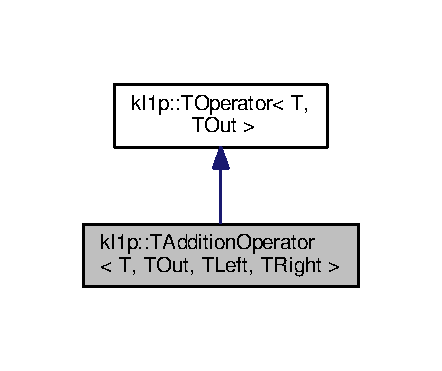
\includegraphics[width=212pt]{classkl1p_1_1TAdditionOperator__inherit__graph}
\end{center}
\end{figure}


Collaboration diagram for kl1p\+:\+:T\+Addition\+Operator$<$ T, T\+Out, T\+Left, T\+Right $>$\+:
\nopagebreak
\begin{figure}[H]
\begin{center}
\leavevmode
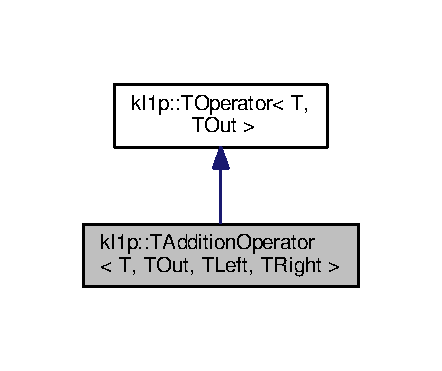
\includegraphics[width=212pt]{classkl1p_1_1TAdditionOperator__coll__graph}
\end{center}
\end{figure}
\subsection*{Public Member Functions}
\begin{DoxyCompactItemize}
\item 
{\bfseries T\+Addition\+Operator} (klab\+::\+T\+Smart\+Pointer$<$ T\+Left $>$ left, klab\+::\+T\+Smart\+Pointer$<$ T\+Right $>$ right)\hypertarget{classkl1p_1_1TAdditionOperator_ae48d781ea7488b1162d83666b36e887e}{}\label{classkl1p_1_1TAdditionOperator_ae48d781ea7488b1162d83666b36e887e}

\item 
{\bfseries T\+Addition\+Operator} (const \hyperlink{classkl1p_1_1TAdditionOperator}{T\+Addition\+Operator}$<$ T, T\+Out, T\+Left, T\+Right $>$ \&op)\hypertarget{classkl1p_1_1TAdditionOperator_a5122e7ccb15ed359a9c745aa40c8d255}{}\label{classkl1p_1_1TAdditionOperator_a5122e7ccb15ed359a9c745aa40c8d255}

\item 
klab\+::\+T\+Smart\+Pointer$<$ T\+Left $>$ {\bfseries left} () const \hypertarget{classkl1p_1_1TAdditionOperator_ad1eb4454f7eab0092ae1d9c008cb6c86}{}\label{classkl1p_1_1TAdditionOperator_ad1eb4454f7eab0092ae1d9c008cb6c86}

\item 
klab\+::\+T\+Smart\+Pointer$<$ T\+Right $>$ {\bfseries right} () const \hypertarget{classkl1p_1_1TAdditionOperator_ae8b9b2d30bcdd7aa6ec91e62d2178287}{}\label{classkl1p_1_1TAdditionOperator_ae8b9b2d30bcdd7aa6ec91e62d2178287}

\item 
virtual bool {\bfseries is\+Zero} ()\hypertarget{classkl1p_1_1TAdditionOperator_afad4f1318aa73bedcce30510f854683d}{}\label{classkl1p_1_1TAdditionOperator_afad4f1318aa73bedcce30510f854683d}

\item 
virtual void {\bfseries apply} (const arma\+::\+Col$<$ T $>$ \&in, arma\+::\+Col$<$ T\+Out $>$ \&out)\hypertarget{classkl1p_1_1TAdditionOperator_ab7e87a2f9dbbafdd1d431e21f6be12c3}{}\label{classkl1p_1_1TAdditionOperator_ab7e87a2f9dbbafdd1d431e21f6be12c3}

\item 
virtual void {\bfseries apply\+Adjoint} (const arma\+::\+Col$<$ T\+Out $>$ \&in, arma\+::\+Col$<$ T $>$ \&out)\hypertarget{classkl1p_1_1TAdditionOperator_a7c9e9c1115ab76c9431dda3633655978}{}\label{classkl1p_1_1TAdditionOperator_a7c9e9c1115ab76c9431dda3633655978}

\item 
virtual void {\bfseries column} (klab\+::\+U\+Int32 i, arma\+::\+Col$<$ T\+Out $>$ \&out)\hypertarget{classkl1p_1_1TAdditionOperator_ae6adca8b253f5f6421ebf4b1dc24decb}{}\label{classkl1p_1_1TAdditionOperator_ae6adca8b253f5f6421ebf4b1dc24decb}

\item 
virtual void {\bfseries column\+Adjoint} (klab\+::\+U\+Int32 i, arma\+::\+Col$<$ T $>$ \&out)\hypertarget{classkl1p_1_1TAdditionOperator_ae38a23526e8749b90cb09cf77957262a}{}\label{classkl1p_1_1TAdditionOperator_ae38a23526e8749b90cb09cf77957262a}

\end{DoxyCompactItemize}
\subsection*{Additional Inherited Members}


The documentation for this class was generated from the following file\+:\begin{DoxyCompactItemize}
\item 
include/Addition\+Operator.\+h\end{DoxyCompactItemize}

\hypertarget{classkl1p_1_1TAdjointBlockOperator}{}\section{kl1p\+:\+:T\+Adjoint\+Block\+Operator$<$ T, T\+Out, T\+Op, T\+Block\+Op, T\+Block $>$ Class Template Reference}
\label{classkl1p_1_1TAdjointBlockOperator}\index{kl1p\+::\+T\+Adjoint\+Block\+Operator$<$ T, T\+Out, T\+Op, T\+Block\+Op, T\+Block $>$@{kl1p\+::\+T\+Adjoint\+Block\+Operator$<$ T, T\+Out, T\+Op, T\+Block\+Op, T\+Block $>$}}


Inheritance diagram for kl1p\+:\+:T\+Adjoint\+Block\+Operator$<$ T, T\+Out, T\+Op, T\+Block\+Op, T\+Block $>$\+:
\nopagebreak
\begin{figure}[H]
\begin{center}
\leavevmode
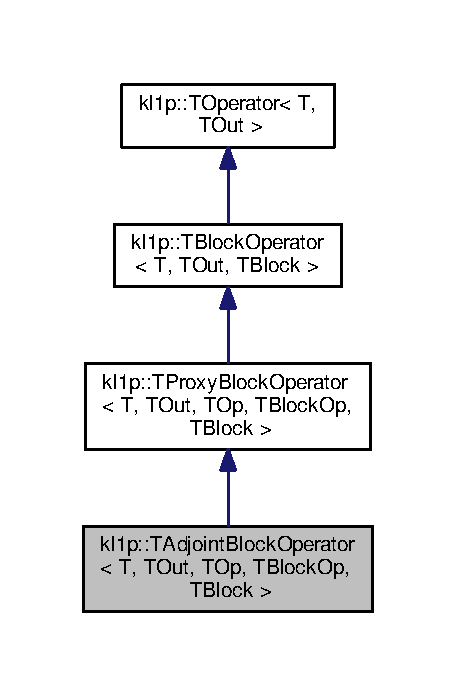
\includegraphics[width=219pt]{classkl1p_1_1TAdjointBlockOperator__inherit__graph}
\end{center}
\end{figure}


Collaboration diagram for kl1p\+:\+:T\+Adjoint\+Block\+Operator$<$ T, T\+Out, T\+Op, T\+Block\+Op, T\+Block $>$\+:
\nopagebreak
\begin{figure}[H]
\begin{center}
\leavevmode
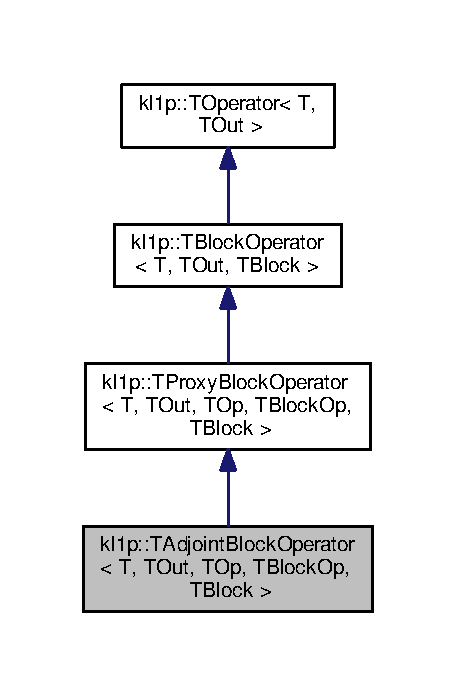
\includegraphics[width=219pt]{classkl1p_1_1TAdjointBlockOperator__coll__graph}
\end{center}
\end{figure}
\subsection*{Public Member Functions}
\begin{DoxyCompactItemize}
\item 
{\bfseries T\+Adjoint\+Block\+Operator} (klab\+::\+T\+Smart\+Pointer$<$ T\+Block\+Op $>$ op)\hypertarget{classkl1p_1_1TAdjointBlockOperator_ad174b513d1bbabdcc129a10aea904291}{}\label{classkl1p_1_1TAdjointBlockOperator_ad174b513d1bbabdcc129a10aea904291}

\item 
{\bfseries T\+Adjoint\+Block\+Operator} (const \hyperlink{classkl1p_1_1TAdjointBlockOperator}{T\+Adjoint\+Block\+Operator}$<$ T, T\+Out, T\+Op, T\+Block\+Op, T\+Block $>$ \&op)\hypertarget{classkl1p_1_1TAdjointBlockOperator_a96c27098ec64506e57941cc5fdee11ce}{}\label{classkl1p_1_1TAdjointBlockOperator_a96c27098ec64506e57941cc5fdee11ce}

\item 
virtual T {\bfseries sum} ()\hypertarget{classkl1p_1_1TAdjointBlockOperator_a0de8ff7ee0f79309d3a4b4d083f3a92c}{}\label{classkl1p_1_1TAdjointBlockOperator_a0de8ff7ee0f79309d3a4b4d083f3a92c}

\item 
virtual T {\bfseries norm\+Frobenius} ()\hypertarget{classkl1p_1_1TAdjointBlockOperator_ad8fae840d0e1718c4ed0258b33ebc22a}{}\label{classkl1p_1_1TAdjointBlockOperator_ad8fae840d0e1718c4ed0258b33ebc22a}

\item 
virtual T {\bfseries squared\+Norm\+Frobenius} ()\hypertarget{classkl1p_1_1TAdjointBlockOperator_a913d9700feba48bfec716025e813b1b6}{}\label{classkl1p_1_1TAdjointBlockOperator_a913d9700feba48bfec716025e813b1b6}

\item 
virtual T {\bfseries mean} ()\hypertarget{classkl1p_1_1TAdjointBlockOperator_a857605ab70a17b91833fe04036481946}{}\label{classkl1p_1_1TAdjointBlockOperator_a857605ab70a17b91833fe04036481946}

\item 
virtual T {\bfseries variance} ()\hypertarget{classkl1p_1_1TAdjointBlockOperator_ac3e42771190da51ed66ebcfc1db2629d}{}\label{classkl1p_1_1TAdjointBlockOperator_ac3e42771190da51ed66ebcfc1db2629d}

\item 
virtual klab\+::\+U\+Int32 {\bfseries count\+Block\+Rows} () const \hypertarget{classkl1p_1_1TAdjointBlockOperator_aa8209652742e0fcfe134aef6d0e71118}{}\label{classkl1p_1_1TAdjointBlockOperator_aa8209652742e0fcfe134aef6d0e71118}

\item 
virtual klab\+::\+U\+Int32 {\bfseries count\+Block\+Columns} () const \hypertarget{classkl1p_1_1TAdjointBlockOperator_ae93a962d58a0af39712acda072e048ac}{}\label{classkl1p_1_1TAdjointBlockOperator_ae93a962d58a0af39712acda072e048ac}

\item 
virtual klab\+::\+T\+Smart\+Pointer$<$ T\+Block $>$ {\bfseries block} (klab\+::\+U\+Int32 i, klab\+::\+U\+Int32 j) const \hypertarget{classkl1p_1_1TAdjointBlockOperator_afd0d7a1b84b1f7296a406ce47bd02909}{}\label{classkl1p_1_1TAdjointBlockOperator_afd0d7a1b84b1f7296a406ce47bd02909}

\item 
virtual bool {\bfseries is\+Zero\+Block} (klab\+::\+U\+Int32 i, klab\+::\+U\+Int32 j) const \hypertarget{classkl1p_1_1TAdjointBlockOperator_aa9c6f62a664a5bdfcde67485d8f9bec2}{}\label{classkl1p_1_1TAdjointBlockOperator_aa9c6f62a664a5bdfcde67485d8f9bec2}

\item 
virtual klab\+::\+T\+Smart\+Pointer$<$ T\+Block $>$ {\bfseries in\+Block} (klab\+::\+U\+Int32 i, klab\+::\+U\+Int32 j) const \hypertarget{classkl1p_1_1TAdjointBlockOperator_a7a1661f7e9abaabd5e5223cecd9754fd}{}\label{classkl1p_1_1TAdjointBlockOperator_a7a1661f7e9abaabd5e5223cecd9754fd}

\item 
virtual void {\bfseries apply} (const arma\+::\+Col$<$ T $>$ \&in, arma\+::\+Col$<$ T\+Out $>$ \&out)\hypertarget{classkl1p_1_1TAdjointBlockOperator_ac6013539ab0af0af5fb3620f998417ed}{}\label{classkl1p_1_1TAdjointBlockOperator_ac6013539ab0af0af5fb3620f998417ed}

\item 
virtual void {\bfseries apply\+Adjoint} (const arma\+::\+Col$<$ T\+Out $>$ \&in, arma\+::\+Col$<$ T $>$ \&out)\hypertarget{classkl1p_1_1TAdjointBlockOperator_adf8456be199079565f31d0c1ba0d3736}{}\label{classkl1p_1_1TAdjointBlockOperator_adf8456be199079565f31d0c1ba0d3736}

\item 
virtual void {\bfseries column} (klab\+::\+U\+Int32 i, arma\+::\+Col$<$ T\+Out $>$ \&out)\hypertarget{classkl1p_1_1TAdjointBlockOperator_a68e3e719ebdb36388ad9f021af11987e}{}\label{classkl1p_1_1TAdjointBlockOperator_a68e3e719ebdb36388ad9f021af11987e}

\item 
virtual void {\bfseries column\+Adjoint} (klab\+::\+U\+Int32 i, arma\+::\+Col$<$ T $>$ \&out)\hypertarget{classkl1p_1_1TAdjointBlockOperator_ab23a40c5eabcb4211975516c3a27ac74}{}\label{classkl1p_1_1TAdjointBlockOperator_ab23a40c5eabcb4211975516c3a27ac74}

\item 
virtual void {\bfseries apply\+Block\+Variance} (const arma\+::\+Col$<$ T $>$ \&in, arma\+::\+Col$<$ T $>$ \&out)\hypertarget{classkl1p_1_1TAdjointBlockOperator_a2d86c03ba6216a82b6276f13f6ac9b59}{}\label{classkl1p_1_1TAdjointBlockOperator_a2d86c03ba6216a82b6276f13f6ac9b59}

\item 
virtual void {\bfseries apply\+Block\+Variance\+Adjoint} (const arma\+::\+Col$<$ T $>$ \&in, arma\+::\+Col$<$ T $>$ \&out)\hypertarget{classkl1p_1_1TAdjointBlockOperator_acc06c3143b5de268ca95c09ab577926a}{}\label{classkl1p_1_1TAdjointBlockOperator_acc06c3143b5de268ca95c09ab577926a}

\end{DoxyCompactItemize}
\subsection*{Additional Inherited Members}


The documentation for this class was generated from the following file\+:\begin{DoxyCompactItemize}
\item 
include/Adjoint\+Block\+Operator.\+h\end{DoxyCompactItemize}

\hypertarget{classkl1p_1_1TAdjointOperator}{}\section{kl1p\+:\+:T\+Adjoint\+Operator$<$ T, T\+Out, T\+Op $>$ Class Template Reference}
\label{classkl1p_1_1TAdjointOperator}\index{kl1p\+::\+T\+Adjoint\+Operator$<$ T, T\+Out, T\+Op $>$@{kl1p\+::\+T\+Adjoint\+Operator$<$ T, T\+Out, T\+Op $>$}}


Inheritance diagram for kl1p\+:\+:T\+Adjoint\+Operator$<$ T, T\+Out, T\+Op $>$\+:
\nopagebreak
\begin{figure}[H]
\begin{center}
\leavevmode
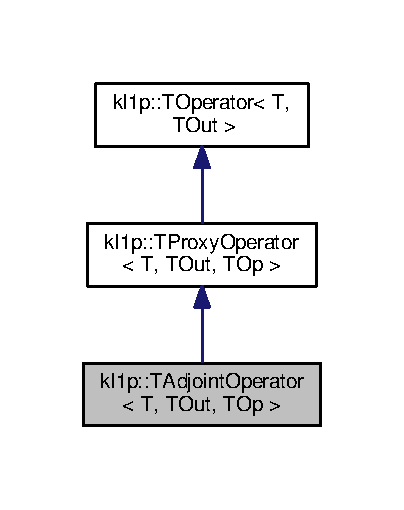
\includegraphics[width=194pt]{classkl1p_1_1TAdjointOperator__inherit__graph}
\end{center}
\end{figure}


Collaboration diagram for kl1p\+:\+:T\+Adjoint\+Operator$<$ T, T\+Out, T\+Op $>$\+:
\nopagebreak
\begin{figure}[H]
\begin{center}
\leavevmode
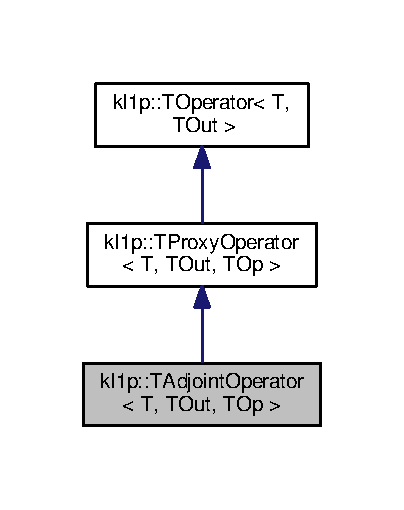
\includegraphics[width=194pt]{classkl1p_1_1TAdjointOperator__coll__graph}
\end{center}
\end{figure}
\subsection*{Public Member Functions}
\begin{DoxyCompactItemize}
\item 
{\bfseries T\+Adjoint\+Operator} (klab\+::\+T\+Smart\+Pointer$<$ T\+Op $>$ op)\hypertarget{classkl1p_1_1TAdjointOperator_a8e918c720c43916849e3b8e7c7d651ad}{}\label{classkl1p_1_1TAdjointOperator_a8e918c720c43916849e3b8e7c7d651ad}

\item 
{\bfseries T\+Adjoint\+Operator} (const \hyperlink{classkl1p_1_1TAdjointOperator}{T\+Adjoint\+Operator}$<$ T, T\+Out, T\+Op $>$ \&op)\hypertarget{classkl1p_1_1TAdjointOperator_ac91c13b95d8cf024186ad2339f37a9bd}{}\label{classkl1p_1_1TAdjointOperator_ac91c13b95d8cf024186ad2339f37a9bd}

\item 
virtual T {\bfseries sum} ()\hypertarget{classkl1p_1_1TAdjointOperator_a02576547b1785c3e26074fb1b1466034}{}\label{classkl1p_1_1TAdjointOperator_a02576547b1785c3e26074fb1b1466034}

\item 
virtual T {\bfseries norm\+Frobenius} ()\hypertarget{classkl1p_1_1TAdjointOperator_a6b11f3ed65e7b5a3efb84392a0bf3469}{}\label{classkl1p_1_1TAdjointOperator_a6b11f3ed65e7b5a3efb84392a0bf3469}

\item 
virtual T {\bfseries squared\+Norm\+Frobenius} ()\hypertarget{classkl1p_1_1TAdjointOperator_a6b539d6725fde5e6106e73a52377dc6f}{}\label{classkl1p_1_1TAdjointOperator_a6b539d6725fde5e6106e73a52377dc6f}

\item 
virtual T {\bfseries mean} ()\hypertarget{classkl1p_1_1TAdjointOperator_a3a01f76abe52501b9567e72bf3b9c1cc}{}\label{classkl1p_1_1TAdjointOperator_a3a01f76abe52501b9567e72bf3b9c1cc}

\item 
virtual T {\bfseries variance} ()\hypertarget{classkl1p_1_1TAdjointOperator_a38ef44746cc7c4d1368f7916fb3033ca}{}\label{classkl1p_1_1TAdjointOperator_a38ef44746cc7c4d1368f7916fb3033ca}

\item 
virtual void {\bfseries apply} (const arma\+::\+Col$<$ T $>$ \&in, arma\+::\+Col$<$ T\+Out $>$ \&out)\hypertarget{classkl1p_1_1TAdjointOperator_a0b1d3c2b9364cfe1b3625096c203c651}{}\label{classkl1p_1_1TAdjointOperator_a0b1d3c2b9364cfe1b3625096c203c651}

\item 
virtual void {\bfseries apply\+Adjoint} (const arma\+::\+Col$<$ T\+Out $>$ \&in, arma\+::\+Col$<$ T $>$ \&out)\hypertarget{classkl1p_1_1TAdjointOperator_ac568d0f9750cb76b6f9993760a360230}{}\label{classkl1p_1_1TAdjointOperator_ac568d0f9750cb76b6f9993760a360230}

\item 
virtual void {\bfseries column} (klab\+::\+U\+Int32 i, arma\+::\+Col$<$ T\+Out $>$ \&out)\hypertarget{classkl1p_1_1TAdjointOperator_a0f7b1596f88594ce81119b3d4e18eda7}{}\label{classkl1p_1_1TAdjointOperator_a0f7b1596f88594ce81119b3d4e18eda7}

\item 
virtual void {\bfseries column\+Adjoint} (klab\+::\+U\+Int32 i, arma\+::\+Col$<$ T $>$ \&out)\hypertarget{classkl1p_1_1TAdjointOperator_af380221ef9538fe31689c6e8b97fabb1}{}\label{classkl1p_1_1TAdjointOperator_af380221ef9538fe31689c6e8b97fabb1}

\end{DoxyCompactItemize}
\subsection*{Additional Inherited Members}


The documentation for this class was generated from the following file\+:\begin{DoxyCompactItemize}
\item 
include/Adjoint\+Operator.\+h\end{DoxyCompactItemize}

\hypertarget{classkl1p_1_1TAMPHistoryElement}{}\section{kl1p\+:\+:T\+A\+M\+P\+History\+Element$<$ T $>$ Class Template Reference}
\label{classkl1p_1_1TAMPHistoryElement}\index{kl1p\+::\+T\+A\+M\+P\+History\+Element$<$ T $>$@{kl1p\+::\+T\+A\+M\+P\+History\+Element$<$ T $>$}}
\subsection*{Public Member Functions}
\begin{DoxyCompactItemize}
\item 
{\bfseries T\+A\+M\+P\+History\+Element} (const T \&residual\+Norm)\hypertarget{classkl1p_1_1TAMPHistoryElement_ab82bfe2b9f73b9277839340ceaad4368}{}\label{classkl1p_1_1TAMPHistoryElement_ab82bfe2b9f73b9277839340ceaad4368}

\item 
{\bfseries T\+A\+M\+P\+History\+Element} (const \hyperlink{classkl1p_1_1TAMPHistoryElement}{T\+A\+M\+P\+History\+Element}$<$ T $>$ \&element)\hypertarget{classkl1p_1_1TAMPHistoryElement_aff2cad4a3376842692fbc80903578615}{}\label{classkl1p_1_1TAMPHistoryElement_aff2cad4a3376842692fbc80903578615}

\item 
\hyperlink{classkl1p_1_1TAMPHistoryElement}{T\+A\+M\+P\+History\+Element}$<$ T $>$ \& {\bfseries operator=} (const \hyperlink{classkl1p_1_1TAMPHistoryElement}{T\+A\+M\+P\+History\+Element}$<$ T $>$ \&element)\hypertarget{classkl1p_1_1TAMPHistoryElement_ab000e1b3add93053e3d046564dc0a53c}{}\label{classkl1p_1_1TAMPHistoryElement_ab000e1b3add93053e3d046564dc0a53c}

\item 
const T \& {\bfseries residual\+Norm} () const \hypertarget{classkl1p_1_1TAMPHistoryElement_abafcf905c37abbe1f0c30d15e409b91a}{}\label{classkl1p_1_1TAMPHistoryElement_abafcf905c37abbe1f0c30d15e409b91a}

\end{DoxyCompactItemize}


The documentation for this class was generated from the following file\+:\begin{DoxyCompactItemize}
\item 
include/A\+M\+P\+History\+Element.\+h\end{DoxyCompactItemize}

\hypertarget{classkl1p_1_1TAMPSolver}{}\section{kl1p\+:\+:T\+A\+M\+P\+Solver$<$ T, T\+Col, T\+Op $>$ Class Template Reference}
\label{classkl1p_1_1TAMPSolver}\index{kl1p\+::\+T\+A\+M\+P\+Solver$<$ T, T\+Col, T\+Op $>$@{kl1p\+::\+T\+A\+M\+P\+Solver$<$ T, T\+Col, T\+Op $>$}}
\subsection*{Public Member Functions}
\begin{DoxyCompactItemize}
\item 
{\bfseries T\+A\+M\+P\+Solver} (const T \&tolerance)\hypertarget{classkl1p_1_1TAMPSolver_a8409842b12ad1edd21a6d757005420bd}{}\label{classkl1p_1_1TAMPSolver_a8409842b12ad1edd21a6d757005420bd}

\item 
{\bfseries T\+A\+M\+P\+Solver} (const T \&tolerance, klab\+::\+U\+Int32 iteration\+Limit)\hypertarget{classkl1p_1_1TAMPSolver_a5076577f06cf910da3db3e197f88b08c}{}\label{classkl1p_1_1TAMPSolver_a5076577f06cf910da3db3e197f88b08c}

\item 
{\bfseries T\+A\+M\+P\+Solver} (const \hyperlink{classkl1p_1_1TAMPSolver}{T\+A\+M\+P\+Solver}$<$ T, T\+Col, T\+Op $>$ \&solver)\hypertarget{classkl1p_1_1TAMPSolver_a46023d22997d73219aeb98b64f141917}{}\label{classkl1p_1_1TAMPSolver_a46023d22997d73219aeb98b64f141917}

\item 
\hyperlink{classkl1p_1_1TAMPSolver}{T\+A\+M\+P\+Solver}$<$ T, T\+Col, T\+Op $>$ \& {\bfseries operator=} (const \hyperlink{classkl1p_1_1TAMPSolver}{T\+A\+M\+P\+Solver}$<$ T, T\+Col, T\+Op $>$ \&solver)\hypertarget{classkl1p_1_1TAMPSolver_aec9102de62ccfcf0bdf4cec34353348d}{}\label{classkl1p_1_1TAMPSolver_aec9102de62ccfcf0bdf4cec34353348d}

\item 
void {\bfseries set\+Tolerance} (const T \&tolerance)\hypertarget{classkl1p_1_1TAMPSolver_a5bb0c3c4917479acc14c799b7edfcd7f}{}\label{classkl1p_1_1TAMPSolver_a5bb0c3c4917479acc14c799b7edfcd7f}

\item 
void {\bfseries set\+Iteration\+Limit} (klab\+::\+U\+Int32 iteration\+Limit)\hypertarget{classkl1p_1_1TAMPSolver_ab4dc6dd8b2bd6c316a1df1c257e8accf}{}\label{classkl1p_1_1TAMPSolver_ab4dc6dd8b2bd6c316a1df1c257e8accf}

\item 
const T \& {\bfseries tolerance} () const \hypertarget{classkl1p_1_1TAMPSolver_a9b6ed85a78ab1987d63976b1599e7bc6}{}\label{classkl1p_1_1TAMPSolver_a9b6ed85a78ab1987d63976b1599e7bc6}

\item 
klab\+::\+U\+Int32 {\bfseries iteration\+Limit} () const \hypertarget{classkl1p_1_1TAMPSolver_aa5679f298008e150cf90fdf3780907c8}{}\label{classkl1p_1_1TAMPSolver_aa5679f298008e150cf90fdf3780907c8}

\item 
const T \& {\bfseries residual\+Norm} () const \hypertarget{classkl1p_1_1TAMPSolver_a4889a7dffbee0f4aac7a2c28730db173}{}\label{classkl1p_1_1TAMPSolver_a4889a7dffbee0f4aac7a2c28730db173}

\item 
const T \& {\bfseries relative\+Residual\+Norm} () const \hypertarget{classkl1p_1_1TAMPSolver_af7f8d281285484a0732a827438f50eb6}{}\label{classkl1p_1_1TAMPSolver_af7f8d281285484a0732a827438f50eb6}

\item 
klab\+::\+U\+Int32 {\bfseries iterations} () const \hypertarget{classkl1p_1_1TAMPSolver_ab8efcd660edc5f18364ded2c1cbe1d49}{}\label{classkl1p_1_1TAMPSolver_ab8efcd660edc5f18364ded2c1cbe1d49}

\item 
void {\bfseries enable\+History} (bool enable)\hypertarget{classkl1p_1_1TAMPSolver_adee60c9920d0108d0143f7d7a7eb1cf1}{}\label{classkl1p_1_1TAMPSolver_adee60c9920d0108d0143f7d7a7eb1cf1}

\item 
bool {\bfseries is\+History\+Enabled} () const \hypertarget{classkl1p_1_1TAMPSolver_ab0ebae5b2b394b051a779d95f82a7b45}{}\label{classkl1p_1_1TAMPSolver_ab0ebae5b2b394b051a779d95f82a7b45}

\item 
const \hyperlink{classkl1p_1_1THistory}{T\+History}$<$ \hyperlink{classkl1p_1_1TAMPHistoryElement}{T\+A\+M\+P\+History\+Element}$<$ T $>$ $>$ \& {\bfseries history} () const \hypertarget{classkl1p_1_1TAMPSolver_ac26f3cbf3b4d21f8446016ecd32de314}{}\label{classkl1p_1_1TAMPSolver_ac26f3cbf3b4d21f8446016ecd32de314}

\item 
void {\bfseries solve} (const arma\+::\+Col$<$ T\+Col $>$ \&y, klab\+::\+T\+Smart\+Pointer$<$ T\+Op $>$ phi, arma\+::\+Col$<$ T\+Col $>$ \&x)\hypertarget{classkl1p_1_1TAMPSolver_a83cab6fbf7939183d1070fd8c98f2024}{}\label{classkl1p_1_1TAMPSolver_a83cab6fbf7939183d1070fd8c98f2024}

\item 
void {\bfseries solve} (const arma\+::\+Col$<$ T\+Col $>$ \&y, klab\+::\+T\+Smart\+Pointer$<$ T\+Op $>$ phi, klab\+::\+T\+Smart\+Pointer$<$ T\+Op $>$ phiT, arma\+::\+Col$<$ T\+Col $>$ \&x)\hypertarget{classkl1p_1_1TAMPSolver_a98617efc42da15d10cc3a8f6d1af6d02}{}\label{classkl1p_1_1TAMPSolver_a98617efc42da15d10cc3a8f6d1af6d02}

\end{DoxyCompactItemize}


The documentation for this class was generated from the following file\+:\begin{DoxyCompactItemize}
\item 
include/A\+M\+P\+Solver.\+h\end{DoxyCompactItemize}

\hypertarget{classkl1p_1_1TBasisPursuitHistoryElement}{}\section{kl1p\+:\+:T\+Basis\+Pursuit\+History\+Element$<$ T $>$ Class Template Reference}
\label{classkl1p_1_1TBasisPursuitHistoryElement}\index{kl1p\+::\+T\+Basis\+Pursuit\+History\+Element$<$ T $>$@{kl1p\+::\+T\+Basis\+Pursuit\+History\+Element$<$ T $>$}}
\subsection*{Public Member Functions}
\begin{DoxyCompactItemize}
\item 
{\bfseries T\+Basis\+Pursuit\+History\+Element} (const T \&residual\+Norm, const T \&duality\+Gap)\hypertarget{classkl1p_1_1TBasisPursuitHistoryElement_afa1fa8219795d180da3d9b7ac7eddecd}{}\label{classkl1p_1_1TBasisPursuitHistoryElement_afa1fa8219795d180da3d9b7ac7eddecd}

\item 
{\bfseries T\+Basis\+Pursuit\+History\+Element} (const \hyperlink{classkl1p_1_1TBasisPursuitHistoryElement}{T\+Basis\+Pursuit\+History\+Element}$<$ T $>$ \&element)\hypertarget{classkl1p_1_1TBasisPursuitHistoryElement_a358e6a35301bb001bd04f94bc4700935}{}\label{classkl1p_1_1TBasisPursuitHistoryElement_a358e6a35301bb001bd04f94bc4700935}

\item 
\hyperlink{classkl1p_1_1TBasisPursuitHistoryElement}{T\+Basis\+Pursuit\+History\+Element}$<$ T $>$ \& {\bfseries operator=} (const \hyperlink{classkl1p_1_1TBasisPursuitHistoryElement}{T\+Basis\+Pursuit\+History\+Element}$<$ T $>$ \&element)\hypertarget{classkl1p_1_1TBasisPursuitHistoryElement_af976517e351cc0a367f9511bd39b7e92}{}\label{classkl1p_1_1TBasisPursuitHistoryElement_af976517e351cc0a367f9511bd39b7e92}

\item 
const T \& {\bfseries residual\+Norm} () const \hypertarget{classkl1p_1_1TBasisPursuitHistoryElement_a64ba00c3c01b40d86e0659d157db32b4}{}\label{classkl1p_1_1TBasisPursuitHistoryElement_a64ba00c3c01b40d86e0659d157db32b4}

\item 
const T \& {\bfseries duality\+Gap} () const \hypertarget{classkl1p_1_1TBasisPursuitHistoryElement_a17f9926a84b231424a29e7742dc2287e}{}\label{classkl1p_1_1TBasisPursuitHistoryElement_a17f9926a84b231424a29e7742dc2287e}

\end{DoxyCompactItemize}


The documentation for this class was generated from the following file\+:\begin{DoxyCompactItemize}
\item 
include/Basis\+Pursuit\+History\+Element.\+h\end{DoxyCompactItemize}

\hypertarget{classkl1p_1_1TBasisPursuitSolver}{}\section{kl1p\+:\+:T\+Basis\+Pursuit\+Solver$<$ T, T\+Col, T\+Op $>$ Class Template Reference}
\label{classkl1p_1_1TBasisPursuitSolver}\index{kl1p\+::\+T\+Basis\+Pursuit\+Solver$<$ T, T\+Col, T\+Op $>$@{kl1p\+::\+T\+Basis\+Pursuit\+Solver$<$ T, T\+Col, T\+Op $>$}}
\subsection*{Public Member Functions}
\begin{DoxyCompactItemize}
\item 
{\bfseries T\+Basis\+Pursuit\+Solver} (const T \&tolerance)\hypertarget{classkl1p_1_1TBasisPursuitSolver_abd12099eb0e9b9d135883ff752c5fee9}{}\label{classkl1p_1_1TBasisPursuitSolver_abd12099eb0e9b9d135883ff752c5fee9}

\item 
{\bfseries T\+Basis\+Pursuit\+Solver} (const T \&tolerance, klab\+::\+U\+Int32 iteration\+Limit)\hypertarget{classkl1p_1_1TBasisPursuitSolver_a4980542f6709c0a9ca157c74dd6a8ae3}{}\label{classkl1p_1_1TBasisPursuitSolver_a4980542f6709c0a9ca157c74dd6a8ae3}

\item 
{\bfseries T\+Basis\+Pursuit\+Solver} (const T \&tolerance, klab\+::\+U\+Int32 iteration\+Limit, klab\+::\+U\+Int32 backtracking\+Iteration\+Limit)\hypertarget{classkl1p_1_1TBasisPursuitSolver_aa3715e94e22870bba29d2b57eeaf96d0}{}\label{classkl1p_1_1TBasisPursuitSolver_aa3715e94e22870bba29d2b57eeaf96d0}

\item 
{\bfseries T\+Basis\+Pursuit\+Solver} (const \hyperlink{classkl1p_1_1TBasisPursuitSolver}{T\+Basis\+Pursuit\+Solver}$<$ T, T\+Col, T\+Op $>$ \&solver)\hypertarget{classkl1p_1_1TBasisPursuitSolver_ab28de8b87231ccbbbab55ee852576daa}{}\label{classkl1p_1_1TBasisPursuitSolver_ab28de8b87231ccbbbab55ee852576daa}

\item 
\hyperlink{classkl1p_1_1TBasisPursuitSolver}{T\+Basis\+Pursuit\+Solver}$<$ T, T\+Col, T\+Op $>$ \& {\bfseries operator=} (const \hyperlink{classkl1p_1_1TBasisPursuitSolver}{T\+Basis\+Pursuit\+Solver}$<$ T, T\+Col, T\+Op $>$ \&solver)\hypertarget{classkl1p_1_1TBasisPursuitSolver_a10d9657dd7a0f8669fcba1c556ccd04f}{}\label{classkl1p_1_1TBasisPursuitSolver_a10d9657dd7a0f8669fcba1c556ccd04f}

\item 
void {\bfseries set\+Tolerance} (const T \&tolerance)\hypertarget{classkl1p_1_1TBasisPursuitSolver_ab4471d1e86105f65aa92bf2405a6b9ad}{}\label{classkl1p_1_1TBasisPursuitSolver_ab4471d1e86105f65aa92bf2405a6b9ad}

\item 
void {\bfseries set\+Iteration\+Limit} (klab\+::\+U\+Int32 iteration\+Limit)\hypertarget{classkl1p_1_1TBasisPursuitSolver_aad318a17bc437dd2c0e71edd15193114}{}\label{classkl1p_1_1TBasisPursuitSolver_aad318a17bc437dd2c0e71edd15193114}

\item 
void {\bfseries set\+Backtracking\+Iteration\+Limit} (klab\+::\+U\+Int32 iteration\+Limit)\hypertarget{classkl1p_1_1TBasisPursuitSolver_a572ea61db1a0111021560b1e40055377}{}\label{classkl1p_1_1TBasisPursuitSolver_a572ea61db1a0111021560b1e40055377}

\item 
void {\bfseries set\+Alpha} (const T \&alpha)\hypertarget{classkl1p_1_1TBasisPursuitSolver_add5e955f35c3de94bf8a1cafe96c6cb7}{}\label{classkl1p_1_1TBasisPursuitSolver_add5e955f35c3de94bf8a1cafe96c6cb7}

\item 
void {\bfseries set\+Beta} (const T \&beta)\hypertarget{classkl1p_1_1TBasisPursuitSolver_aef8f810999b29096c966715b3531963c}{}\label{classkl1p_1_1TBasisPursuitSolver_aef8f810999b29096c966715b3531963c}

\item 
void {\bfseries set\+Mu} (const T \&mu)\hypertarget{classkl1p_1_1TBasisPursuitSolver_a4079b0c20309a5253e047eaf1c40d189}{}\label{classkl1p_1_1TBasisPursuitSolver_a4079b0c20309a5253e047eaf1c40d189}

\item 
const T \& {\bfseries tolerance} () const \hypertarget{classkl1p_1_1TBasisPursuitSolver_ad015cf6bcfae17dd6367e85bea99a359}{}\label{classkl1p_1_1TBasisPursuitSolver_ad015cf6bcfae17dd6367e85bea99a359}

\item 
klab\+::\+U\+Int32 {\bfseries iteration\+Limit} () const \hypertarget{classkl1p_1_1TBasisPursuitSolver_ad1f36fa34392dd4b11ab75e32ccc756f}{}\label{classkl1p_1_1TBasisPursuitSolver_ad1f36fa34392dd4b11ab75e32ccc756f}

\item 
klab\+::\+U\+Int32 {\bfseries backtracking\+Iteration\+Limit} () const \hypertarget{classkl1p_1_1TBasisPursuitSolver_a706f7502e62afedac139a4ba3347db87}{}\label{classkl1p_1_1TBasisPursuitSolver_a706f7502e62afedac139a4ba3347db87}

\item 
const T \& {\bfseries alpha} () const \hypertarget{classkl1p_1_1TBasisPursuitSolver_a5b9f19b29f6d8591f60bc5b6f34a2e8f}{}\label{classkl1p_1_1TBasisPursuitSolver_a5b9f19b29f6d8591f60bc5b6f34a2e8f}

\item 
const T \& {\bfseries beta} () const \hypertarget{classkl1p_1_1TBasisPursuitSolver_a53177da0be730b3c0f51952eb6a2b62e}{}\label{classkl1p_1_1TBasisPursuitSolver_a53177da0be730b3c0f51952eb6a2b62e}

\item 
const T \& {\bfseries mu} () const \hypertarget{classkl1p_1_1TBasisPursuitSolver_a6fa8b3b05714f3db166dab61a7ecc750}{}\label{classkl1p_1_1TBasisPursuitSolver_a6fa8b3b05714f3db166dab61a7ecc750}

\item 
const T \& {\bfseries residual\+Norm} () const \hypertarget{classkl1p_1_1TBasisPursuitSolver_ab923202f79f0fb19230aa463cf4bc173}{}\label{classkl1p_1_1TBasisPursuitSolver_ab923202f79f0fb19230aa463cf4bc173}

\item 
const T \& {\bfseries relative\+Residual\+Norm} () const \hypertarget{classkl1p_1_1TBasisPursuitSolver_ade8c6cd21c29a8028911e13790f659f0}{}\label{classkl1p_1_1TBasisPursuitSolver_ade8c6cd21c29a8028911e13790f659f0}

\item 
const T \& {\bfseries duality\+Gap} () const \hypertarget{classkl1p_1_1TBasisPursuitSolver_a81a56c29993fb3feef82d3f6b716a009}{}\label{classkl1p_1_1TBasisPursuitSolver_a81a56c29993fb3feef82d3f6b716a009}

\item 
klab\+::\+U\+Int32 {\bfseries iterations} () const \hypertarget{classkl1p_1_1TBasisPursuitSolver_acf53c7752ba2ed1c573e996c1f90cdb7}{}\label{classkl1p_1_1TBasisPursuitSolver_acf53c7752ba2ed1c573e996c1f90cdb7}

\item 
const klab\+::\+T\+Conjugate\+Gradient\+System\+Solver$<$ T, T\+Col $>$ \& {\bfseries conjugate\+Gradient\+Solver} () const \hypertarget{classkl1p_1_1TBasisPursuitSolver_aeb3ea7af0f6f7b814e0c9d95dadc1af4}{}\label{classkl1p_1_1TBasisPursuitSolver_aeb3ea7af0f6f7b814e0c9d95dadc1af4}

\item 
klab\+::\+T\+Conjugate\+Gradient\+System\+Solver$<$ T, T\+Col $>$ \& {\bfseries conjugate\+Gradient\+Solver} ()\hypertarget{classkl1p_1_1TBasisPursuitSolver_aebed416d290328172c6cc5f59a8b03fd}{}\label{classkl1p_1_1TBasisPursuitSolver_aebed416d290328172c6cc5f59a8b03fd}

\item 
void {\bfseries enable\+History} (bool enable)\hypertarget{classkl1p_1_1TBasisPursuitSolver_ac9fe5b6619fd6aea0375b0a90d0a497c}{}\label{classkl1p_1_1TBasisPursuitSolver_ac9fe5b6619fd6aea0375b0a90d0a497c}

\item 
bool {\bfseries is\+History\+Enabled} () const \hypertarget{classkl1p_1_1TBasisPursuitSolver_a594183ddd3592c96101802bb6228b996}{}\label{classkl1p_1_1TBasisPursuitSolver_a594183ddd3592c96101802bb6228b996}

\item 
const \hyperlink{classkl1p_1_1THistory}{T\+History}$<$ \hyperlink{classkl1p_1_1TBasisPursuitHistoryElement}{T\+Basis\+Pursuit\+History\+Element}$<$ T $>$ $>$ \& {\bfseries history} () const \hypertarget{classkl1p_1_1TBasisPursuitSolver_a090cafd2a97a7916a057dd96eb7a00ad}{}\label{classkl1p_1_1TBasisPursuitSolver_a090cafd2a97a7916a057dd96eb7a00ad}

\item 
void {\bfseries solve} (const arma\+::\+Col$<$ T\+Col $>$ \&y, klab\+::\+T\+Smart\+Pointer$<$ T\+Op $>$ phi, arma\+::\+Col$<$ T\+Col $>$ \&x)\hypertarget{classkl1p_1_1TBasisPursuitSolver_a40c6219b30228f89ddc562944ca0de25}{}\label{classkl1p_1_1TBasisPursuitSolver_a40c6219b30228f89ddc562944ca0de25}

\item 
void {\bfseries solve} (const arma\+::\+Col$<$ T\+Col $>$ \&y, klab\+::\+T\+Smart\+Pointer$<$ T\+Op $>$ phi, klab\+::\+T\+Smart\+Pointer$<$ T\+Op $>$ phiT, arma\+::\+Col$<$ T\+Col $>$ \&x)\hypertarget{classkl1p_1_1TBasisPursuitSolver_a9c8558fc3903e0281d2d9bf9ec38fc3c}{}\label{classkl1p_1_1TBasisPursuitSolver_a9c8558fc3903e0281d2d9bf9ec38fc3c}

\end{DoxyCompactItemize}
\subsection*{Protected Member Functions}
\begin{DoxyCompactItemize}
\item 
void {\bfseries solve\+\_\+\+Real\+Version} (const arma\+::\+Col$<$ T\+Col $>$ \&y, klab\+::\+T\+Smart\+Pointer$<$ T\+Op $>$ phi, klab\+::\+T\+Smart\+Pointer$<$ T\+Op $>$ phiT, arma\+::\+Col$<$ T\+Col $>$ \&x, T \&residual\+Norm, T \&relative\+Residual\+Norm, T \&sdg, klab\+::\+U\+Int32 \&iterations, \hyperlink{classkl1p_1_1THistory}{T\+History}$<$ \hyperlink{classkl1p_1_1TBasisPursuitHistoryElement}{T\+Basis\+Pursuit\+History\+Element}$<$ T $>$ $>$ \&history)\hypertarget{classkl1p_1_1TBasisPursuitSolver_a667e83828792e2fef99dd7870f50bff8}{}\label{classkl1p_1_1TBasisPursuitSolver_a667e83828792e2fef99dd7870f50bff8}

\end{DoxyCompactItemize}
\subsection*{Static Protected Member Functions}
\begin{DoxyCompactItemize}
\item 
static T\+Col {\bfseries Compute\+Step\+Value} (const arma\+::\+Col$<$ T\+Col $>$ \&fu1, const arma\+::\+Col$<$ T\+Col $>$ \&fu2, const arma\+::\+Col$<$ T\+Col $>$ \&lambda\+U1, const arma\+::\+Col$<$ T\+Col $>$ \&lambda\+U2, const arma\+::\+Col$<$ T\+Col $>$ \&d\+Lambda\+U1, const arma\+::\+Col$<$ T\+Col $>$ \&d\+Lambda\+U2, const arma\+::\+Col$<$ T\+Col $>$ \&dx, const arma\+::\+Col$<$ T\+Col $>$ \&du)\hypertarget{classkl1p_1_1TBasisPursuitSolver_a59d51c64c9062dddbd444e06a8c3937f}{}\label{classkl1p_1_1TBasisPursuitSolver_a59d51c64c9062dddbd444e06a8c3937f}

\end{DoxyCompactItemize}
\subsection*{Friends}
\begin{DoxyCompactItemize}
\item 
{\footnotesize template$<$class U , class U\+Col , class U\+Op $>$ }\\class {\bfseries T\+Basis\+Pursuit\+Solver\+Specialisation}\hypertarget{classkl1p_1_1TBasisPursuitSolver_ab1c111a48736ffa667f87545df6cc15d}{}\label{classkl1p_1_1TBasisPursuitSolver_ab1c111a48736ffa667f87545df6cc15d}

\end{DoxyCompactItemize}


The documentation for this class was generated from the following file\+:\begin{DoxyCompactItemize}
\item 
include/Basis\+Pursuit\+Solver.\+h\end{DoxyCompactItemize}

\hypertarget{classkl1p_1_1TBasisPursuitSolverSpecialisation}{}\section{kl1p\+:\+:T\+Basis\+Pursuit\+Solver\+Specialisation$<$ T, T\+Col, T\+Op $>$ Class Template Reference}
\label{classkl1p_1_1TBasisPursuitSolverSpecialisation}\index{kl1p\+::\+T\+Basis\+Pursuit\+Solver\+Specialisation$<$ T, T\+Col, T\+Op $>$@{kl1p\+::\+T\+Basis\+Pursuit\+Solver\+Specialisation$<$ T, T\+Col, T\+Op $>$}}
\subsection*{Static Public Member Functions}
\begin{DoxyCompactItemize}
\item 
static void {\bfseries Solve} (const arma\+::\+Col$<$ T\+Col $>$ \&y, klab\+::\+T\+Smart\+Pointer$<$ T\+Op $>$ phi, klab\+::\+T\+Smart\+Pointer$<$ T\+Op $>$ phiT, arma\+::\+Col$<$ T\+Col $>$ \&x, \hyperlink{classkl1p_1_1TBasisPursuitSolver}{T\+Basis\+Pursuit\+Solver}$<$ T, T\+Col, T\+Op $>$ \&solver)\hypertarget{classkl1p_1_1TBasisPursuitSolverSpecialisation_a613b9b642f603608c7c9a199f5b9d0a4}{}\label{classkl1p_1_1TBasisPursuitSolverSpecialisation_a613b9b642f603608c7c9a199f5b9d0a4}

\end{DoxyCompactItemize}


The documentation for this class was generated from the following file\+:\begin{DoxyCompactItemize}
\item 
include/Basis\+Pursuit\+Solver.\+h\end{DoxyCompactItemize}

\hypertarget{classkl1p_1_1TBasisPursuitSolverSpecialisation_3_01T_00_01std_1_1complex_3_01TCol_01_4_00_01TOp_01_4}{}\section{kl1p\+:\+:T\+Basis\+Pursuit\+Solver\+Specialisation$<$ T, std\+:\+:complex$<$ T\+Col $>$, T\+Op $>$ Class Template Reference}
\label{classkl1p_1_1TBasisPursuitSolverSpecialisation_3_01T_00_01std_1_1complex_3_01TCol_01_4_00_01TOp_01_4}\index{kl1p\+::\+T\+Basis\+Pursuit\+Solver\+Specialisation$<$ T, std\+::complex$<$ T\+Col $>$, T\+Op $>$@{kl1p\+::\+T\+Basis\+Pursuit\+Solver\+Specialisation$<$ T, std\+::complex$<$ T\+Col $>$, T\+Op $>$}}
\subsection*{Static Public Member Functions}
\begin{DoxyCompactItemize}
\item 
static void {\bfseries Solve} (const arma\+::\+Col$<$ std\+::complex$<$ T\+Col $>$ $>$ \&y, klab\+::\+T\+Smart\+Pointer$<$ T\+Op $>$ phi, klab\+::\+T\+Smart\+Pointer$<$ T\+Op $>$ phiT, arma\+::\+Col$<$ std\+::complex$<$ T\+Col $>$ $>$ \&x, \hyperlink{classkl1p_1_1TBasisPursuitSolver}{T\+Basis\+Pursuit\+Solver}$<$ T, std\+::complex$<$ T\+Col $>$, T\+Op $>$ \&solver)\hypertarget{classkl1p_1_1TBasisPursuitSolverSpecialisation_3_01T_00_01std_1_1complex_3_01TCol_01_4_00_01TOp_01_4_a4ff909f734a724391631287f7785b0e5}{}\label{classkl1p_1_1TBasisPursuitSolverSpecialisation_3_01T_00_01std_1_1complex_3_01TCol_01_4_00_01TOp_01_4_a4ff909f734a724391631287f7785b0e5}

\end{DoxyCompactItemize}


The documentation for this class was generated from the following file\+:\begin{DoxyCompactItemize}
\item 
include/Basis\+Pursuit\+Solver.\+h\end{DoxyCompactItemize}

\hypertarget{classkl1p_1_1TBlockDiagonalOperator}{}\section{kl1p\+:\+:T\+Block\+Diagonal\+Operator$<$ T, T\+Out, T\+Op $>$ Class Template Reference}
\label{classkl1p_1_1TBlockDiagonalOperator}\index{kl1p\+::\+T\+Block\+Diagonal\+Operator$<$ T, T\+Out, T\+Op $>$@{kl1p\+::\+T\+Block\+Diagonal\+Operator$<$ T, T\+Out, T\+Op $>$}}


Inheritance diagram for kl1p\+:\+:T\+Block\+Diagonal\+Operator$<$ T, T\+Out, T\+Op $>$\+:
\nopagebreak
\begin{figure}[H]
\begin{center}
\leavevmode
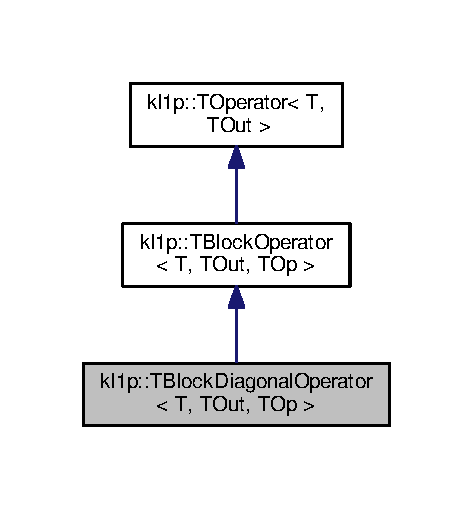
\includegraphics[width=227pt]{classkl1p_1_1TBlockDiagonalOperator__inherit__graph}
\end{center}
\end{figure}


Collaboration diagram for kl1p\+:\+:T\+Block\+Diagonal\+Operator$<$ T, T\+Out, T\+Op $>$\+:
\nopagebreak
\begin{figure}[H]
\begin{center}
\leavevmode
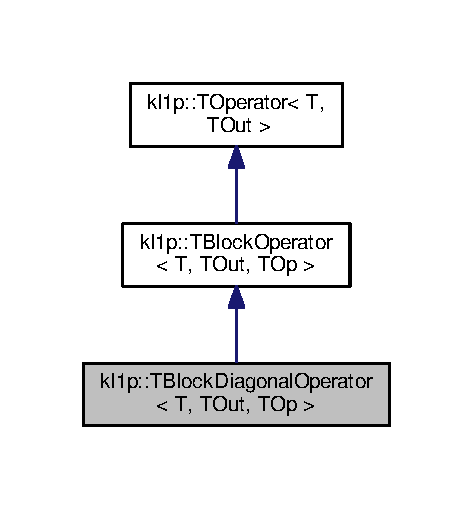
\includegraphics[width=227pt]{classkl1p_1_1TBlockDiagonalOperator__coll__graph}
\end{center}
\end{figure}
\subsection*{Public Types}
\begin{DoxyCompactItemize}
\item 
typedef std\+::vector$<$ klab\+::\+T\+Smart\+Pointer$<$ T\+Op $>$ $>$ {\bfseries T\+Operator\+Array}\hypertarget{classkl1p_1_1TBlockDiagonalOperator_ad33c7b4cfd584979cb34b4f5c51a16d8}{}\label{classkl1p_1_1TBlockDiagonalOperator_ad33c7b4cfd584979cb34b4f5c51a16d8}

\end{DoxyCompactItemize}
\subsection*{Public Member Functions}
\begin{DoxyCompactItemize}
\item 
{\bfseries T\+Block\+Diagonal\+Operator} (klab\+::\+T\+Smart\+Pointer$<$ T\+Op $>$ op)\hypertarget{classkl1p_1_1TBlockDiagonalOperator_a5bb117d84b4ab6f24b7ed3d537f32d84}{}\label{classkl1p_1_1TBlockDiagonalOperator_a5bb117d84b4ab6f24b7ed3d537f32d84}

\item 
{\bfseries T\+Block\+Diagonal\+Operator} (klab\+::\+T\+Smart\+Pointer$<$ T\+Op $>$ op1, klab\+::\+T\+Smart\+Pointer$<$ T\+Op $>$ op2)\hypertarget{classkl1p_1_1TBlockDiagonalOperator_a3208a2a7d63f6295e24c9f591f4c8f25}{}\label{classkl1p_1_1TBlockDiagonalOperator_a3208a2a7d63f6295e24c9f591f4c8f25}

\item 
{\bfseries T\+Block\+Diagonal\+Operator} (klab\+::\+T\+Smart\+Pointer$<$ T\+Op $>$ op1, klab\+::\+T\+Smart\+Pointer$<$ T\+Op $>$ op2, klab\+::\+T\+Smart\+Pointer$<$ T\+Op $>$ op3)\hypertarget{classkl1p_1_1TBlockDiagonalOperator_a0a5391de470f2d94b87675c1f9d08dd0}{}\label{classkl1p_1_1TBlockDiagonalOperator_a0a5391de470f2d94b87675c1f9d08dd0}

\item 
{\bfseries T\+Block\+Diagonal\+Operator} (const typename \hyperlink{classkl1p_1_1TBlockDiagonalOperator}{T\+Block\+Diagonal\+Operator}$<$ T, T\+Out, T\+Op $>$\+::T\+Operator\+Array \&ops)\hypertarget{classkl1p_1_1TBlockDiagonalOperator_a51eca6f49e3b9eddcd4cbe98e43bd428}{}\label{classkl1p_1_1TBlockDiagonalOperator_a51eca6f49e3b9eddcd4cbe98e43bd428}

\item 
{\bfseries T\+Block\+Diagonal\+Operator} (const \hyperlink{classkl1p_1_1TBlockDiagonalOperator}{T\+Block\+Diagonal\+Operator}$<$ T, T\+Out, T\+Op $>$ \&op)\hypertarget{classkl1p_1_1TBlockDiagonalOperator_a23f424572fd85f8619931c6ceeadee91}{}\label{classkl1p_1_1TBlockDiagonalOperator_a23f424572fd85f8619931c6ceeadee91}

\item 
virtual bool {\bfseries is\+Zero} ()\hypertarget{classkl1p_1_1TBlockDiagonalOperator_a495a43e99ac028c66cfa43d6a8803173}{}\label{classkl1p_1_1TBlockDiagonalOperator_a495a43e99ac028c66cfa43d6a8803173}

\item 
virtual klab\+::\+U\+Int32 {\bfseries count\+Block\+Rows} () const \hypertarget{classkl1p_1_1TBlockDiagonalOperator_a3c84f36c3292ce2dc96550948e336741}{}\label{classkl1p_1_1TBlockDiagonalOperator_a3c84f36c3292ce2dc96550948e336741}

\item 
virtual klab\+::\+U\+Int32 {\bfseries count\+Block\+Columns} () const \hypertarget{classkl1p_1_1TBlockDiagonalOperator_ab5f650485e832010c3bf066e81f7b51c}{}\label{classkl1p_1_1TBlockDiagonalOperator_ab5f650485e832010c3bf066e81f7b51c}

\item 
virtual klab\+::\+T\+Smart\+Pointer$<$ T\+Op $>$ {\bfseries block} (klab\+::\+U\+Int32 i, klab\+::\+U\+Int32 j) const \hypertarget{classkl1p_1_1TBlockDiagonalOperator_ad2faf788f1e5d6582016a01abcd6f421}{}\label{classkl1p_1_1TBlockDiagonalOperator_ad2faf788f1e5d6582016a01abcd6f421}

\item 
virtual bool {\bfseries is\+Zero\+Block} (klab\+::\+U\+Int32 i, klab\+::\+U\+Int32 j) const \hypertarget{classkl1p_1_1TBlockDiagonalOperator_ab87734c38b99e8fdee34a8d470b6a9e0}{}\label{classkl1p_1_1TBlockDiagonalOperator_ab87734c38b99e8fdee34a8d470b6a9e0}

\item 
virtual klab\+::\+T\+Smart\+Pointer$<$ T\+Op $>$ {\bfseries in\+Block} (klab\+::\+U\+Int32 i, klab\+::\+U\+Int32 j) const \hypertarget{classkl1p_1_1TBlockDiagonalOperator_a706f7630da22dfea218065259e215d38}{}\label{classkl1p_1_1TBlockDiagonalOperator_a706f7630da22dfea218065259e215d38}

\item 
virtual void {\bfseries apply} (const arma\+::\+Col$<$ T $>$ \&in, arma\+::\+Col$<$ T\+Out $>$ \&out)\hypertarget{classkl1p_1_1TBlockDiagonalOperator_a3f34f696160cf9818dfb86a04bfd4c41}{}\label{classkl1p_1_1TBlockDiagonalOperator_a3f34f696160cf9818dfb86a04bfd4c41}

\item 
virtual void {\bfseries apply\+Adjoint} (const arma\+::\+Col$<$ T\+Out $>$ \&in, arma\+::\+Col$<$ T $>$ \&out)\hypertarget{classkl1p_1_1TBlockDiagonalOperator_acf69f8652502cdabcbf4aa56f3ac9262}{}\label{classkl1p_1_1TBlockDiagonalOperator_acf69f8652502cdabcbf4aa56f3ac9262}

\item 
virtual void {\bfseries column} (klab\+::\+U\+Int32 i, arma\+::\+Col$<$ T\+Out $>$ \&out)\hypertarget{classkl1p_1_1TBlockDiagonalOperator_a7281190bf92d50ea8261874d426a39eb}{}\label{classkl1p_1_1TBlockDiagonalOperator_a7281190bf92d50ea8261874d426a39eb}

\item 
virtual void {\bfseries column\+Adjoint} (klab\+::\+U\+Int32 i, arma\+::\+Col$<$ T $>$ \&out)\hypertarget{classkl1p_1_1TBlockDiagonalOperator_a37b1264646d5cfb5a3981e176be44d14}{}\label{classkl1p_1_1TBlockDiagonalOperator_a37b1264646d5cfb5a3981e176be44d14}

\item 
virtual void {\bfseries apply\+Block\+Variance} (const arma\+::\+Col$<$ T $>$ \&in, arma\+::\+Col$<$ T $>$ \&out)\hypertarget{classkl1p_1_1TBlockDiagonalOperator_aafd45b42f432a8bf57b207c58ce44817}{}\label{classkl1p_1_1TBlockDiagonalOperator_aafd45b42f432a8bf57b207c58ce44817}

\item 
virtual void {\bfseries apply\+Block\+Variance\+Adjoint} (const arma\+::\+Col$<$ T $>$ \&in, arma\+::\+Col$<$ T $>$ \&out)\hypertarget{classkl1p_1_1TBlockDiagonalOperator_aa8d9ac9d10de8b125eb2fcc19dd12ffa}{}\label{classkl1p_1_1TBlockDiagonalOperator_aa8d9ac9d10de8b125eb2fcc19dd12ffa}

\end{DoxyCompactItemize}
\subsection*{Protected Member Functions}
\begin{DoxyCompactItemize}
\item 
void {\bfseries update\+Variance\+Matrix} ()\hypertarget{classkl1p_1_1TBlockDiagonalOperator_ac91ba0e41a0bb6420c591198493a2ea9}{}\label{classkl1p_1_1TBlockDiagonalOperator_ac91ba0e41a0bb6420c591198493a2ea9}

\end{DoxyCompactItemize}


The documentation for this class was generated from the following file\+:\begin{DoxyCompactItemize}
\item 
include/Block\+Diagonal\+Operator.\+h\end{DoxyCompactItemize}

\hypertarget{classkl1p_1_1TBlockOperator}{}\section{kl1p\+:\+:T\+Block\+Operator$<$ T, T\+Out, T\+Op $>$ Class Template Reference}
\label{classkl1p_1_1TBlockOperator}\index{kl1p\+::\+T\+Block\+Operator$<$ T, T\+Out, T\+Op $>$@{kl1p\+::\+T\+Block\+Operator$<$ T, T\+Out, T\+Op $>$}}


Inheritance diagram for kl1p\+:\+:T\+Block\+Operator$<$ T, T\+Out, T\+Op $>$\+:
\nopagebreak
\begin{figure}[H]
\begin{center}
\leavevmode
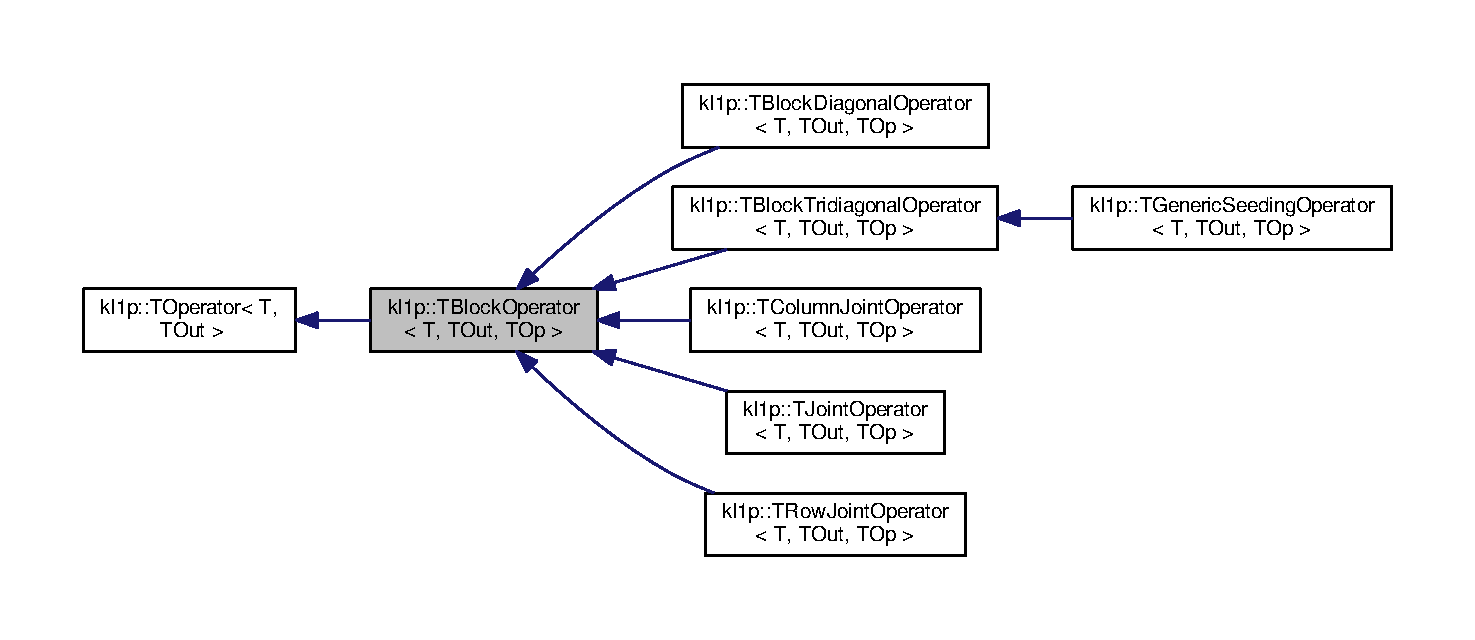
\includegraphics[width=350pt]{classkl1p_1_1TBlockOperator__inherit__graph}
\end{center}
\end{figure}


Collaboration diagram for kl1p\+:\+:T\+Block\+Operator$<$ T, T\+Out, T\+Op $>$\+:
\nopagebreak
\begin{figure}[H]
\begin{center}
\leavevmode
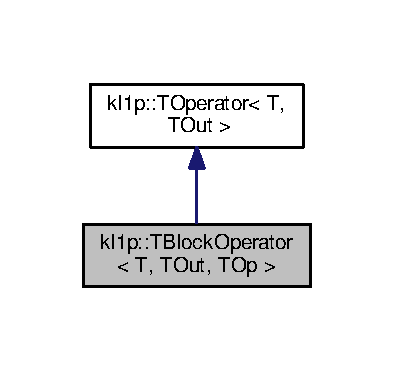
\includegraphics[width=189pt]{classkl1p_1_1TBlockOperator__coll__graph}
\end{center}
\end{figure}
\subsection*{Public Member Functions}
\begin{DoxyCompactItemize}
\item 
{\bfseries T\+Block\+Operator} (klab\+::\+U\+Int32 n)\hypertarget{classkl1p_1_1TBlockOperator_a5dc354ba1f729db43de46140a32e3026}{}\label{classkl1p_1_1TBlockOperator_a5dc354ba1f729db43de46140a32e3026}

\item 
{\bfseries T\+Block\+Operator} (klab\+::\+U\+Int32 m, klab\+::\+U\+Int32 n)\hypertarget{classkl1p_1_1TBlockOperator_a582054d812e2fa198041c0f4b49650f9}{}\label{classkl1p_1_1TBlockOperator_a582054d812e2fa198041c0f4b49650f9}

\item 
{\bfseries T\+Block\+Operator} (const \hyperlink{classkl1p_1_1TBlockOperator}{T\+Block\+Operator}$<$ T, T\+Out, T\+Op $>$ \&op)\hypertarget{classkl1p_1_1TBlockOperator_a6f125a341d84ddecd00aee2ac163b869}{}\label{classkl1p_1_1TBlockOperator_a6f125a341d84ddecd00aee2ac163b869}

\item 
virtual bool {\bfseries is\+Zero} ()\hypertarget{classkl1p_1_1TBlockOperator_a0dc821bb4c6b6a4d83f8116980068361}{}\label{classkl1p_1_1TBlockOperator_a0dc821bb4c6b6a4d83f8116980068361}

\item 
virtual T {\bfseries sum} ()\hypertarget{classkl1p_1_1TBlockOperator_af94660a9ae9a441e534242d8a1341324}{}\label{classkl1p_1_1TBlockOperator_af94660a9ae9a441e534242d8a1341324}

\item 
virtual T {\bfseries squared\+Norm\+Frobenius} ()\hypertarget{classkl1p_1_1TBlockOperator_a6bf4b8cceb7591a14910178adc41399e}{}\label{classkl1p_1_1TBlockOperator_a6bf4b8cceb7591a14910178adc41399e}

\item 
virtual klab\+::\+U\+Int32 {\bfseries count\+Block\+Rows} () const =0\hypertarget{classkl1p_1_1TBlockOperator_a11b06e07e2caddb5ce6e02b84ee1f9a7}{}\label{classkl1p_1_1TBlockOperator_a11b06e07e2caddb5ce6e02b84ee1f9a7}

\item 
virtual klab\+::\+U\+Int32 {\bfseries count\+Block\+Columns} () const =0\hypertarget{classkl1p_1_1TBlockOperator_a3ee4a1fcb3ccb494cb2fac7cc2d454ee}{}\label{classkl1p_1_1TBlockOperator_a3ee4a1fcb3ccb494cb2fac7cc2d454ee}

\item 
virtual klab\+::\+T\+Smart\+Pointer$<$ T\+Op $>$ {\bfseries block} (klab\+::\+U\+Int32 i, klab\+::\+U\+Int32 j) const =0\hypertarget{classkl1p_1_1TBlockOperator_a818d8197561091b57eb68da45984e862}{}\label{classkl1p_1_1TBlockOperator_a818d8197561091b57eb68da45984e862}

\item 
virtual bool {\bfseries is\+Zero\+Block} (klab\+::\+U\+Int32 i, klab\+::\+U\+Int32 j) const \hypertarget{classkl1p_1_1TBlockOperator_a38f14ee4289d3a1022621fd2756468a0}{}\label{classkl1p_1_1TBlockOperator_a38f14ee4289d3a1022621fd2756468a0}

\item 
virtual klab\+::\+T\+Smart\+Pointer$<$ T\+Op $>$ {\bfseries in\+Block} (klab\+::\+U\+Int32 i, klab\+::\+U\+Int32 j) const \hypertarget{classkl1p_1_1TBlockOperator_abe27ac7aae020a0046b41dbbce833c2e}{}\label{classkl1p_1_1TBlockOperator_abe27ac7aae020a0046b41dbbce833c2e}

\item 
virtual void {\bfseries apply} (const arma\+::\+Col$<$ T $>$ \&in, arma\+::\+Col$<$ T\+Out $>$ \&out)\hypertarget{classkl1p_1_1TBlockOperator_abe8347dc36f51357b31019202e6519f6}{}\label{classkl1p_1_1TBlockOperator_abe8347dc36f51357b31019202e6519f6}

\item 
virtual void {\bfseries apply\+Adjoint} (const arma\+::\+Col$<$ T\+Out $>$ \&in, arma\+::\+Col$<$ T $>$ \&out)\hypertarget{classkl1p_1_1TBlockOperator_a16f5ca78ef3004162ed0bec64a33f2a7}{}\label{classkl1p_1_1TBlockOperator_a16f5ca78ef3004162ed0bec64a33f2a7}

\item 
virtual void {\bfseries column} (klab\+::\+U\+Int32 i, arma\+::\+Col$<$ T\+Out $>$ \&out)\hypertarget{classkl1p_1_1TBlockOperator_afd7fe16a9a975d78d04c08f0d4840585}{}\label{classkl1p_1_1TBlockOperator_afd7fe16a9a975d78d04c08f0d4840585}

\item 
virtual void {\bfseries column\+Adjoint} (klab\+::\+U\+Int32 i, arma\+::\+Col$<$ T $>$ \&out)\hypertarget{classkl1p_1_1TBlockOperator_aaba087da87a91484c87e034ca1cb24c8}{}\label{classkl1p_1_1TBlockOperator_aaba087da87a91484c87e034ca1cb24c8}

\item 
virtual void {\bfseries apply\+Block\+Variance} (const arma\+::\+Col$<$ T $>$ \&in, arma\+::\+Col$<$ T $>$ \&out)\hypertarget{classkl1p_1_1TBlockOperator_a9f7a58f4ad532f72761cadb0dcb37ffe}{}\label{classkl1p_1_1TBlockOperator_a9f7a58f4ad532f72761cadb0dcb37ffe}

\item 
virtual void {\bfseries apply\+Block\+Variance\+Adjoint} (const arma\+::\+Col$<$ T $>$ \&in, arma\+::\+Col$<$ T $>$ \&out)\hypertarget{classkl1p_1_1TBlockOperator_aa3603d90acc99c1f6b43578b8701ecb9}{}\label{classkl1p_1_1TBlockOperator_aa3603d90acc99c1f6b43578b8701ecb9}

\end{DoxyCompactItemize}
\subsection*{Additional Inherited Members}


The documentation for this class was generated from the following file\+:\begin{DoxyCompactItemize}
\item 
include/Block\+Operator.\+h\end{DoxyCompactItemize}

\hypertarget{classkl1p_1_1TBlockSparseOperator}{}\section{kl1p\+:\+:T\+Block\+Sparse\+Operator$<$ T, T\+Out, T\+Op $>$ Class Template Reference}
\label{classkl1p_1_1TBlockSparseOperator}\index{kl1p\+::\+T\+Block\+Sparse\+Operator$<$ T, T\+Out, T\+Op $>$@{kl1p\+::\+T\+Block\+Sparse\+Operator$<$ T, T\+Out, T\+Op $>$}}


Inheritance diagram for kl1p\+:\+:T\+Block\+Sparse\+Operator$<$ T, T\+Out, T\+Op $>$\+:
\nopagebreak
\begin{figure}[H]
\begin{center}
\leavevmode
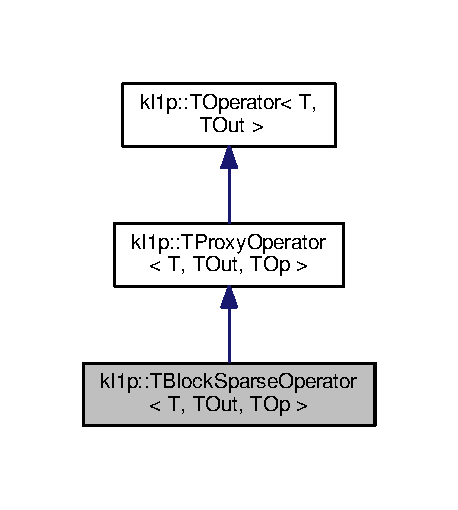
\includegraphics[width=220pt]{classkl1p_1_1TBlockSparseOperator__inherit__graph}
\end{center}
\end{figure}


Collaboration diagram for kl1p\+:\+:T\+Block\+Sparse\+Operator$<$ T, T\+Out, T\+Op $>$\+:
\nopagebreak
\begin{figure}[H]
\begin{center}
\leavevmode
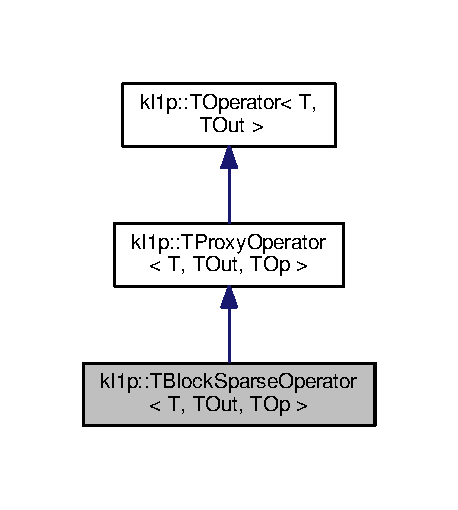
\includegraphics[width=220pt]{classkl1p_1_1TBlockSparseOperator__coll__graph}
\end{center}
\end{figure}
\subsection*{Public Member Functions}
\begin{DoxyCompactItemize}
\item 
{\bfseries T\+Block\+Sparse\+Operator} (klab\+::\+U\+Int32 m, klab\+::\+U\+Int32 n, klab\+::\+T\+Smart\+Pointer$<$ T\+Op $>$ op, klab\+::\+U\+Int32 i=0, klab\+::\+U\+Int32 j=0)\hypertarget{classkl1p_1_1TBlockSparseOperator_af0c2a5bd04d2148f411eea28e14ceef4}{}\label{classkl1p_1_1TBlockSparseOperator_af0c2a5bd04d2148f411eea28e14ceef4}

\item 
{\bfseries T\+Block\+Sparse\+Operator} (const \hyperlink{classkl1p_1_1TBlockSparseOperator}{T\+Block\+Sparse\+Operator}$<$ T, T\+Out, T\+Op $>$ \&op)\hypertarget{classkl1p_1_1TBlockSparseOperator_acbc282b128a473bb7d6089a2e77e446c}{}\label{classkl1p_1_1TBlockSparseOperator_acbc282b128a473bb7d6089a2e77e446c}

\item 
klab\+::\+U\+Int32 {\bfseries i} () const \hypertarget{classkl1p_1_1TBlockSparseOperator_ac4432fa617c2d193eb8ef0c1edb1381c}{}\label{classkl1p_1_1TBlockSparseOperator_ac4432fa617c2d193eb8ef0c1edb1381c}

\item 
klab\+::\+U\+Int32 {\bfseries j} () const \hypertarget{classkl1p_1_1TBlockSparseOperator_a49c572c0c9050c4347e0afbed5565326}{}\label{classkl1p_1_1TBlockSparseOperator_a49c572c0c9050c4347e0afbed5565326}

\item 
virtual void {\bfseries apply} (const arma\+::\+Col$<$ T $>$ \&in, arma\+::\+Col$<$ T\+Out $>$ \&out)\hypertarget{classkl1p_1_1TBlockSparseOperator_ada3066cb198b324d18b5d05ccd5117bc}{}\label{classkl1p_1_1TBlockSparseOperator_ada3066cb198b324d18b5d05ccd5117bc}

\item 
virtual void {\bfseries apply\+Adjoint} (const arma\+::\+Col$<$ T\+Out $>$ \&in, arma\+::\+Col$<$ T $>$ \&out)\hypertarget{classkl1p_1_1TBlockSparseOperator_a18e3069fd6392329c031d650c368914d}{}\label{classkl1p_1_1TBlockSparseOperator_a18e3069fd6392329c031d650c368914d}

\item 
virtual void {\bfseries column} (klab\+::\+U\+Int32 i, arma\+::\+Col$<$ T\+Out $>$ \&out)\hypertarget{classkl1p_1_1TBlockSparseOperator_ac5bb115aa4b1e002b5f3a5751b6674aa}{}\label{classkl1p_1_1TBlockSparseOperator_ac5bb115aa4b1e002b5f3a5751b6674aa}

\item 
virtual void {\bfseries column\+Adjoint} (klab\+::\+U\+Int32 i, arma\+::\+Col$<$ T $>$ \&out)\hypertarget{classkl1p_1_1TBlockSparseOperator_a7c4adcf2d38ce4d11b9d054aef743769}{}\label{classkl1p_1_1TBlockSparseOperator_a7c4adcf2d38ce4d11b9d054aef743769}

\end{DoxyCompactItemize}
\subsection*{Additional Inherited Members}


The documentation for this class was generated from the following file\+:\begin{DoxyCompactItemize}
\item 
include/Block\+Sparse\+Operator.\+h\end{DoxyCompactItemize}

\hypertarget{classkl1p_1_1TBlockTridiagonalOperator}{}\section{kl1p\+:\+:T\+Block\+Tridiagonal\+Operator$<$ T, T\+Out, T\+Op $>$ Class Template Reference}
\label{classkl1p_1_1TBlockTridiagonalOperator}\index{kl1p\+::\+T\+Block\+Tridiagonal\+Operator$<$ T, T\+Out, T\+Op $>$@{kl1p\+::\+T\+Block\+Tridiagonal\+Operator$<$ T, T\+Out, T\+Op $>$}}


Inheritance diagram for kl1p\+:\+:T\+Block\+Tridiagonal\+Operator$<$ T, T\+Out, T\+Op $>$\+:
\nopagebreak
\begin{figure}[H]
\begin{center}
\leavevmode
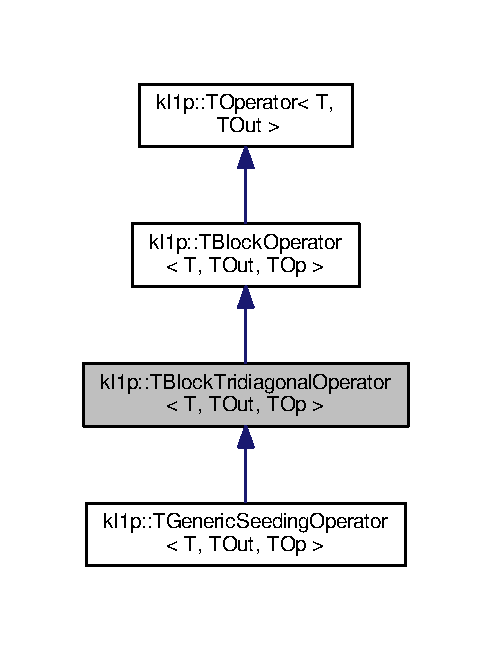
\includegraphics[width=236pt]{classkl1p_1_1TBlockTridiagonalOperator__inherit__graph}
\end{center}
\end{figure}


Collaboration diagram for kl1p\+:\+:T\+Block\+Tridiagonal\+Operator$<$ T, T\+Out, T\+Op $>$\+:
\nopagebreak
\begin{figure}[H]
\begin{center}
\leavevmode
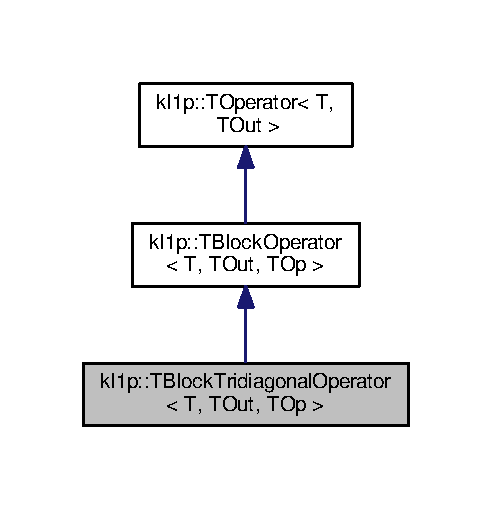
\includegraphics[width=236pt]{classkl1p_1_1TBlockTridiagonalOperator__coll__graph}
\end{center}
\end{figure}
\subsection*{Public Types}
\begin{DoxyCompactItemize}
\item 
typedef std\+::vector$<$ klab\+::\+T\+Smart\+Pointer$<$ T\+Op $>$ $>$ {\bfseries T\+Operator\+Array}\hypertarget{classkl1p_1_1TBlockTridiagonalOperator_a1e93b7a33162d0a67de0c2fbf47d6f9c}{}\label{classkl1p_1_1TBlockTridiagonalOperator_a1e93b7a33162d0a67de0c2fbf47d6f9c}

\end{DoxyCompactItemize}
\subsection*{Public Member Functions}
\begin{DoxyCompactItemize}
\item 
{\bfseries T\+Block\+Tridiagonal\+Operator} (const typename \hyperlink{classkl1p_1_1TBlockTridiagonalOperator}{T\+Block\+Tridiagonal\+Operator}$<$ T, T\+Out, T\+Op $>$\+::T\+Operator\+Array \&diagonal, const typename \hyperlink{classkl1p_1_1TBlockTridiagonalOperator}{T\+Block\+Tridiagonal\+Operator}$<$ T, T\+Out, T\+Op $>$\+::T\+Operator\+Array \&lower, const typename \hyperlink{classkl1p_1_1TBlockTridiagonalOperator}{T\+Block\+Tridiagonal\+Operator}$<$ T, T\+Out, T\+Op $>$\+::T\+Operator\+Array \&upper)\hypertarget{classkl1p_1_1TBlockTridiagonalOperator_a87a7873f0782fb05915f809fc36319da}{}\label{classkl1p_1_1TBlockTridiagonalOperator_a87a7873f0782fb05915f809fc36319da}

\item 
{\bfseries T\+Block\+Tridiagonal\+Operator} (const \hyperlink{classkl1p_1_1TBlockTridiagonalOperator}{T\+Block\+Tridiagonal\+Operator}$<$ T, T\+Out, T\+Op $>$ \&op)\hypertarget{classkl1p_1_1TBlockTridiagonalOperator_aa0adc9ee189b2a204de3c17342b46729}{}\label{classkl1p_1_1TBlockTridiagonalOperator_aa0adc9ee189b2a204de3c17342b46729}

\item 
virtual bool {\bfseries is\+Zero} ()\hypertarget{classkl1p_1_1TBlockTridiagonalOperator_a6a373ba3575c7881967d7073001d810b}{}\label{classkl1p_1_1TBlockTridiagonalOperator_a6a373ba3575c7881967d7073001d810b}

\item 
virtual klab\+::\+U\+Int32 {\bfseries count\+Block\+Rows} () const \hypertarget{classkl1p_1_1TBlockTridiagonalOperator_aac39849319dece38b0634cab0ce861e0}{}\label{classkl1p_1_1TBlockTridiagonalOperator_aac39849319dece38b0634cab0ce861e0}

\item 
virtual klab\+::\+U\+Int32 {\bfseries count\+Block\+Columns} () const \hypertarget{classkl1p_1_1TBlockTridiagonalOperator_aceac6d7a78d22b49164806d78bee6f9f}{}\label{classkl1p_1_1TBlockTridiagonalOperator_aceac6d7a78d22b49164806d78bee6f9f}

\item 
virtual klab\+::\+T\+Smart\+Pointer$<$ T\+Op $>$ {\bfseries block} (klab\+::\+U\+Int32 i, klab\+::\+U\+Int32 j) const \hypertarget{classkl1p_1_1TBlockTridiagonalOperator_a0bc4423406e914e2ad6aa5b81d59ba08}{}\label{classkl1p_1_1TBlockTridiagonalOperator_a0bc4423406e914e2ad6aa5b81d59ba08}

\item 
virtual bool {\bfseries is\+Zero\+Block} (klab\+::\+U\+Int32 i, klab\+::\+U\+Int32 j) const \hypertarget{classkl1p_1_1TBlockTridiagonalOperator_a834b9d95a38de854034c7b097e2f4d09}{}\label{classkl1p_1_1TBlockTridiagonalOperator_a834b9d95a38de854034c7b097e2f4d09}

\item 
virtual klab\+::\+T\+Smart\+Pointer$<$ T\+Op $>$ {\bfseries in\+Block} (klab\+::\+U\+Int32 i, klab\+::\+U\+Int32 j) const \hypertarget{classkl1p_1_1TBlockTridiagonalOperator_af25114ddcc9bcf6361898823c8c84bed}{}\label{classkl1p_1_1TBlockTridiagonalOperator_af25114ddcc9bcf6361898823c8c84bed}

\item 
virtual void {\bfseries apply} (const arma\+::\+Col$<$ T $>$ \&in, arma\+::\+Col$<$ T\+Out $>$ \&out)\hypertarget{classkl1p_1_1TBlockTridiagonalOperator_a1fe3f41ec6f514ca3557e91a157339bd}{}\label{classkl1p_1_1TBlockTridiagonalOperator_a1fe3f41ec6f514ca3557e91a157339bd}

\item 
virtual void {\bfseries apply\+Adjoint} (const arma\+::\+Col$<$ T\+Out $>$ \&in, arma\+::\+Col$<$ T $>$ \&out)\hypertarget{classkl1p_1_1TBlockTridiagonalOperator_a52c61b719ed8123a6f0bd63a17077bc8}{}\label{classkl1p_1_1TBlockTridiagonalOperator_a52c61b719ed8123a6f0bd63a17077bc8}

\item 
virtual void {\bfseries column} (klab\+::\+U\+Int32 i, arma\+::\+Col$<$ T\+Out $>$ \&out)\hypertarget{classkl1p_1_1TBlockTridiagonalOperator_afc94e82c8434e715017709cab88de987}{}\label{classkl1p_1_1TBlockTridiagonalOperator_afc94e82c8434e715017709cab88de987}

\item 
virtual void {\bfseries column\+Adjoint} (klab\+::\+U\+Int32 i, arma\+::\+Col$<$ T $>$ \&out)\hypertarget{classkl1p_1_1TBlockTridiagonalOperator_a11283192c9b22f0113da7a6cc5472f81}{}\label{classkl1p_1_1TBlockTridiagonalOperator_a11283192c9b22f0113da7a6cc5472f81}

\item 
virtual void {\bfseries apply\+Block\+Variance} (const arma\+::\+Col$<$ T $>$ \&in, arma\+::\+Col$<$ T $>$ \&out)\hypertarget{classkl1p_1_1TBlockTridiagonalOperator_a47aa5c4177cfb0c9ea194cfaa7b93cd1}{}\label{classkl1p_1_1TBlockTridiagonalOperator_a47aa5c4177cfb0c9ea194cfaa7b93cd1}

\item 
virtual void {\bfseries apply\+Block\+Variance\+Adjoint} (const arma\+::\+Col$<$ T $>$ \&in, arma\+::\+Col$<$ T $>$ \&out)\hypertarget{classkl1p_1_1TBlockTridiagonalOperator_ae3b88a97c3f8449b3176ecfc1486649f}{}\label{classkl1p_1_1TBlockTridiagonalOperator_ae3b88a97c3f8449b3176ecfc1486649f}

\end{DoxyCompactItemize}
\subsection*{Protected Member Functions}
\begin{DoxyCompactItemize}
\item 
void {\bfseries set\+Tridiagonal\+Arrays} (const typename \hyperlink{classkl1p_1_1TBlockTridiagonalOperator}{T\+Block\+Tridiagonal\+Operator}$<$ T, T\+Out, T\+Op $>$\+::T\+Operator\+Array \&diagonal, const typename \hyperlink{classkl1p_1_1TBlockTridiagonalOperator}{T\+Block\+Tridiagonal\+Operator}$<$ T, T\+Out, T\+Op $>$\+::T\+Operator\+Array \&lower, const typename \hyperlink{classkl1p_1_1TBlockTridiagonalOperator}{T\+Block\+Tridiagonal\+Operator}$<$ T, T\+Out, T\+Op $>$\+::T\+Operator\+Array \&upper)\hypertarget{classkl1p_1_1TBlockTridiagonalOperator_a169465de5cb9fc91276ad0dc0bdee2a4}{}\label{classkl1p_1_1TBlockTridiagonalOperator_a169465de5cb9fc91276ad0dc0bdee2a4}

\item 
void {\bfseries update\+Variance\+Matrix} ()\hypertarget{classkl1p_1_1TBlockTridiagonalOperator_a88049332216e59bd2eca24484b862f0c}{}\label{classkl1p_1_1TBlockTridiagonalOperator_a88049332216e59bd2eca24484b862f0c}

\end{DoxyCompactItemize}


The documentation for this class was generated from the following file\+:\begin{DoxyCompactItemize}
\item 
include/Block\+Tridiagonal\+Operator.\+h\end{DoxyCompactItemize}

\hypertarget{classkl1p_1_1TColumnJointOperator}{}\section{kl1p\+:\+:T\+Column\+Joint\+Operator$<$ T, T\+Out, T\+Op $>$ Class Template Reference}
\label{classkl1p_1_1TColumnJointOperator}\index{kl1p\+::\+T\+Column\+Joint\+Operator$<$ T, T\+Out, T\+Op $>$@{kl1p\+::\+T\+Column\+Joint\+Operator$<$ T, T\+Out, T\+Op $>$}}


Inheritance diagram for kl1p\+:\+:T\+Column\+Joint\+Operator$<$ T, T\+Out, T\+Op $>$\+:
\nopagebreak
\begin{figure}[H]
\begin{center}
\leavevmode
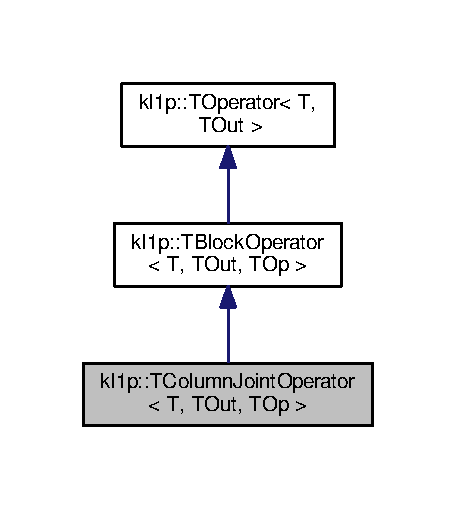
\includegraphics[width=219pt]{classkl1p_1_1TColumnJointOperator__inherit__graph}
\end{center}
\end{figure}


Collaboration diagram for kl1p\+:\+:T\+Column\+Joint\+Operator$<$ T, T\+Out, T\+Op $>$\+:
\nopagebreak
\begin{figure}[H]
\begin{center}
\leavevmode
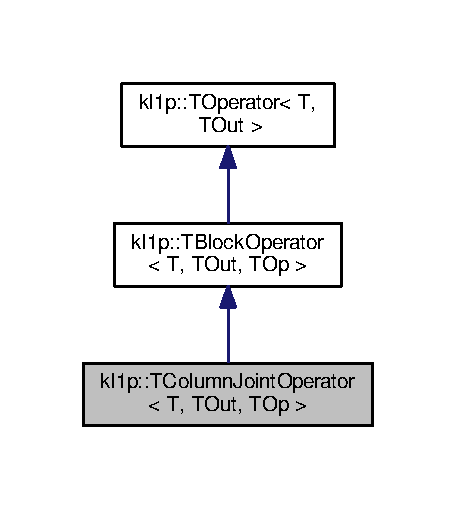
\includegraphics[width=219pt]{classkl1p_1_1TColumnJointOperator__coll__graph}
\end{center}
\end{figure}
\subsection*{Public Types}
\begin{DoxyCompactItemize}
\item 
typedef std\+::vector$<$ klab\+::\+T\+Smart\+Pointer$<$ T\+Op $>$ $>$ {\bfseries T\+Operator\+Array}\hypertarget{classkl1p_1_1TColumnJointOperator_a9d4fd1b1376b19a417cf13ed4fc422e2}{}\label{classkl1p_1_1TColumnJointOperator_a9d4fd1b1376b19a417cf13ed4fc422e2}

\end{DoxyCompactItemize}
\subsection*{Public Member Functions}
\begin{DoxyCompactItemize}
\item 
{\bfseries T\+Column\+Joint\+Operator} (klab\+::\+T\+Smart\+Pointer$<$ T\+Op $>$ op)\hypertarget{classkl1p_1_1TColumnJointOperator_a02082364d2d12a045519698ab5b9a241}{}\label{classkl1p_1_1TColumnJointOperator_a02082364d2d12a045519698ab5b9a241}

\item 
{\bfseries T\+Column\+Joint\+Operator} (klab\+::\+T\+Smart\+Pointer$<$ T\+Op $>$ op1, klab\+::\+T\+Smart\+Pointer$<$ T\+Op $>$ op2)\hypertarget{classkl1p_1_1TColumnJointOperator_ab97fc18b1c3c59df66865512d6839721}{}\label{classkl1p_1_1TColumnJointOperator_ab97fc18b1c3c59df66865512d6839721}

\item 
{\bfseries T\+Column\+Joint\+Operator} (klab\+::\+T\+Smart\+Pointer$<$ T\+Op $>$ op1, klab\+::\+T\+Smart\+Pointer$<$ T\+Op $>$ op2, klab\+::\+T\+Smart\+Pointer$<$ T\+Op $>$ op3)\hypertarget{classkl1p_1_1TColumnJointOperator_ab977246405a98933c73309eaa889df82}{}\label{classkl1p_1_1TColumnJointOperator_ab977246405a98933c73309eaa889df82}

\item 
{\bfseries T\+Column\+Joint\+Operator} (const typename \hyperlink{classkl1p_1_1TColumnJointOperator}{T\+Column\+Joint\+Operator}$<$ T, T\+Out, T\+Op $>$\+::T\+Operator\+Array \&ops)\hypertarget{classkl1p_1_1TColumnJointOperator_a4de54c20174cc3f935c446b5859fcaf8}{}\label{classkl1p_1_1TColumnJointOperator_a4de54c20174cc3f935c446b5859fcaf8}

\item 
{\bfseries T\+Column\+Joint\+Operator} (const \hyperlink{classkl1p_1_1TColumnJointOperator}{T\+Column\+Joint\+Operator}$<$ T, T\+Out, T\+Op $>$ \&op)\hypertarget{classkl1p_1_1TColumnJointOperator_a62e6479533163225e77c0e1b14378e0e}{}\label{classkl1p_1_1TColumnJointOperator_a62e6479533163225e77c0e1b14378e0e}

\item 
virtual bool {\bfseries is\+Zero} ()\hypertarget{classkl1p_1_1TColumnJointOperator_aeb7aff5eb413b3a9aac72a90d4aced9d}{}\label{classkl1p_1_1TColumnJointOperator_aeb7aff5eb413b3a9aac72a90d4aced9d}

\item 
virtual klab\+::\+U\+Int32 {\bfseries count\+Block\+Rows} () const \hypertarget{classkl1p_1_1TColumnJointOperator_a1fc0609bedf1c849bc64f6535d53360a}{}\label{classkl1p_1_1TColumnJointOperator_a1fc0609bedf1c849bc64f6535d53360a}

\item 
virtual klab\+::\+U\+Int32 {\bfseries count\+Block\+Columns} () const \hypertarget{classkl1p_1_1TColumnJointOperator_a6de3a65aa4d4769dfb0eb7556877b2fc}{}\label{classkl1p_1_1TColumnJointOperator_a6de3a65aa4d4769dfb0eb7556877b2fc}

\item 
virtual klab\+::\+T\+Smart\+Pointer$<$ T\+Op $>$ {\bfseries block} (klab\+::\+U\+Int32 i, klab\+::\+U\+Int32 j) const \hypertarget{classkl1p_1_1TColumnJointOperator_a26b5e1eee5a563028fea9605e73e78b6}{}\label{classkl1p_1_1TColumnJointOperator_a26b5e1eee5a563028fea9605e73e78b6}

\item 
virtual bool {\bfseries is\+Zero\+Block} (klab\+::\+U\+Int32 i, klab\+::\+U\+Int32 j) const \hypertarget{classkl1p_1_1TColumnJointOperator_a16e900f678d80c2de31344ab4341b366}{}\label{classkl1p_1_1TColumnJointOperator_a16e900f678d80c2de31344ab4341b366}

\item 
virtual klab\+::\+T\+Smart\+Pointer$<$ T\+Op $>$ {\bfseries in\+Block} (klab\+::\+U\+Int32 i, klab\+::\+U\+Int32 j) const \hypertarget{classkl1p_1_1TColumnJointOperator_ae33cbd4735dfd7e30f1773fe3e875e57}{}\label{classkl1p_1_1TColumnJointOperator_ae33cbd4735dfd7e30f1773fe3e875e57}

\item 
virtual void {\bfseries apply} (const arma\+::\+Col$<$ T $>$ \&in, arma\+::\+Col$<$ T\+Out $>$ \&out)\hypertarget{classkl1p_1_1TColumnJointOperator_a0bd2f7e3656fd14e8328063bde591bc0}{}\label{classkl1p_1_1TColumnJointOperator_a0bd2f7e3656fd14e8328063bde591bc0}

\item 
virtual void {\bfseries apply\+Adjoint} (const arma\+::\+Col$<$ T\+Out $>$ \&in, arma\+::\+Col$<$ T $>$ \&out)\hypertarget{classkl1p_1_1TColumnJointOperator_af15492ac3423bfaad5456c99c8236fb9}{}\label{classkl1p_1_1TColumnJointOperator_af15492ac3423bfaad5456c99c8236fb9}

\item 
virtual void {\bfseries column} (klab\+::\+U\+Int32 i, arma\+::\+Col$<$ T\+Out $>$ \&out)\hypertarget{classkl1p_1_1TColumnJointOperator_a99ac91ff87f6985a9f0f3d6300d54fc4}{}\label{classkl1p_1_1TColumnJointOperator_a99ac91ff87f6985a9f0f3d6300d54fc4}

\item 
virtual void {\bfseries column\+Adjoint} (klab\+::\+U\+Int32 i, arma\+::\+Col$<$ T $>$ \&out)\hypertarget{classkl1p_1_1TColumnJointOperator_a119944332beae5d5005ec2ea872a8d11}{}\label{classkl1p_1_1TColumnJointOperator_a119944332beae5d5005ec2ea872a8d11}

\item 
virtual void {\bfseries apply\+Block\+Variance} (const arma\+::\+Col$<$ T $>$ \&in, arma\+::\+Col$<$ T $>$ \&out)\hypertarget{classkl1p_1_1TColumnJointOperator_a6ba8fc8dd7718501b1bf85dc98e1906c}{}\label{classkl1p_1_1TColumnJointOperator_a6ba8fc8dd7718501b1bf85dc98e1906c}

\item 
virtual void {\bfseries apply\+Block\+Variance\+Adjoint} (const arma\+::\+Col$<$ T $>$ \&in, arma\+::\+Col$<$ T $>$ \&out)\hypertarget{classkl1p_1_1TColumnJointOperator_a7c20b44637b82a4899a7a949ce931adc}{}\label{classkl1p_1_1TColumnJointOperator_a7c20b44637b82a4899a7a949ce931adc}

\end{DoxyCompactItemize}
\subsection*{Protected Member Functions}
\begin{DoxyCompactItemize}
\item 
void {\bfseries update\+Variance\+Matrix} ()\hypertarget{classkl1p_1_1TColumnJointOperator_a7e3d933b298daeb775fd120f712eff28}{}\label{classkl1p_1_1TColumnJointOperator_a7e3d933b298daeb775fd120f712eff28}

\end{DoxyCompactItemize}


The documentation for this class was generated from the following file\+:\begin{DoxyCompactItemize}
\item 
include/Column\+Joint\+Operator.\+h\end{DoxyCompactItemize}

\hypertarget{classkl1p_1_1TComplexProxyBlockOperator}{}\section{kl1p\+:\+:T\+Complex\+Proxy\+Block\+Operator$<$ T, T\+Out, T\+Op, T\+Block\+Op, T\+Block $>$ Class Template Reference}
\label{classkl1p_1_1TComplexProxyBlockOperator}\index{kl1p\+::\+T\+Complex\+Proxy\+Block\+Operator$<$ T, T\+Out, T\+Op, T\+Block\+Op, T\+Block $>$@{kl1p\+::\+T\+Complex\+Proxy\+Block\+Operator$<$ T, T\+Out, T\+Op, T\+Block\+Op, T\+Block $>$}}


Inheritance diagram for kl1p\+:\+:T\+Complex\+Proxy\+Block\+Operator$<$ T, T\+Out, T\+Op, T\+Block\+Op, T\+Block $>$\+:
\nopagebreak
\begin{figure}[H]
\begin{center}
\leavevmode
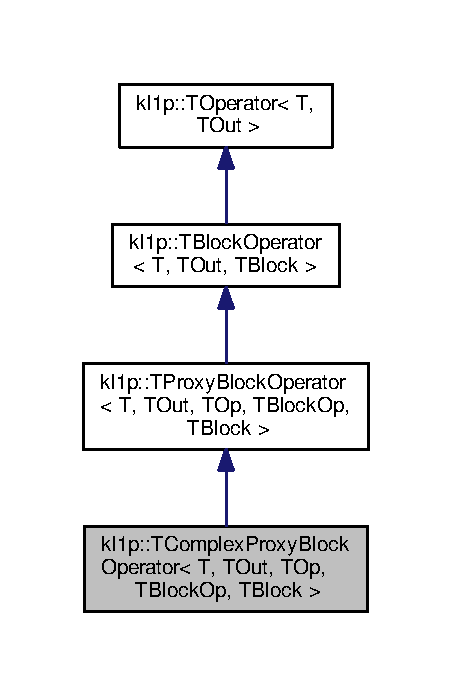
\includegraphics[width=217pt]{classkl1p_1_1TComplexProxyBlockOperator__inherit__graph}
\end{center}
\end{figure}


Collaboration diagram for kl1p\+:\+:T\+Complex\+Proxy\+Block\+Operator$<$ T, T\+Out, T\+Op, T\+Block\+Op, T\+Block $>$\+:
\nopagebreak
\begin{figure}[H]
\begin{center}
\leavevmode
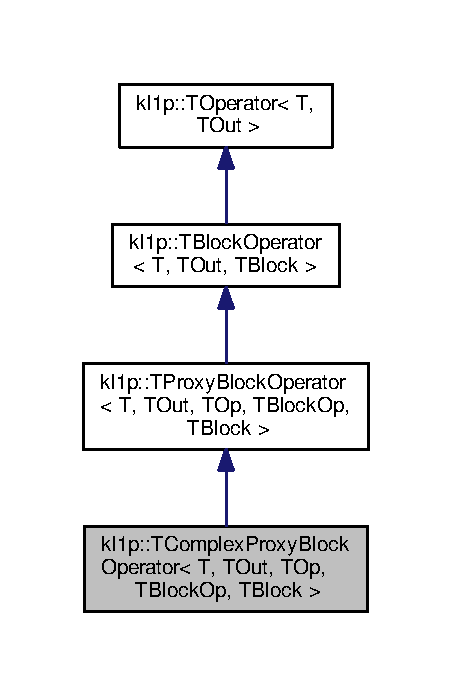
\includegraphics[width=217pt]{classkl1p_1_1TComplexProxyBlockOperator__coll__graph}
\end{center}
\end{figure}
\subsection*{Public Member Functions}
\begin{DoxyCompactItemize}
\item 
{\bfseries T\+Complex\+Proxy\+Block\+Operator} (klab\+::\+T\+Smart\+Pointer$<$ T\+Block\+Op $>$ op)\hypertarget{classkl1p_1_1TComplexProxyBlockOperator_a2f962ad972aaf8f9b4702dd5d80eced9}{}\label{classkl1p_1_1TComplexProxyBlockOperator_a2f962ad972aaf8f9b4702dd5d80eced9}

\item 
{\bfseries T\+Complex\+Proxy\+Block\+Operator} (const \hyperlink{classkl1p_1_1TComplexProxyBlockOperator}{T\+Complex\+Proxy\+Block\+Operator}$<$ T, T\+Out, T\+Op, T\+Block\+Op, T\+Block $>$ \&op)\hypertarget{classkl1p_1_1TComplexProxyBlockOperator_a04722c553f55607508c6526e43ade887}{}\label{classkl1p_1_1TComplexProxyBlockOperator_a04722c553f55607508c6526e43ade887}

\item 
virtual T {\bfseries sum} ()\hypertarget{classkl1p_1_1TComplexProxyBlockOperator_aec11a1961928456a0fcf2d6e9fd72d48}{}\label{classkl1p_1_1TComplexProxyBlockOperator_aec11a1961928456a0fcf2d6e9fd72d48}

\item 
virtual T {\bfseries norm\+Frobenius} ()\hypertarget{classkl1p_1_1TComplexProxyBlockOperator_a3a616c71aca28467321febb8d5df0ab2}{}\label{classkl1p_1_1TComplexProxyBlockOperator_a3a616c71aca28467321febb8d5df0ab2}

\item 
virtual T {\bfseries squared\+Norm\+Frobenius} ()\hypertarget{classkl1p_1_1TComplexProxyBlockOperator_a0e4b35d5b1a497d46d2159f584f5887c}{}\label{classkl1p_1_1TComplexProxyBlockOperator_a0e4b35d5b1a497d46d2159f584f5887c}

\item 
virtual T {\bfseries mean} ()\hypertarget{classkl1p_1_1TComplexProxyBlockOperator_a29ff6ad7e91c57d31dd28c5c556c9dc5}{}\label{classkl1p_1_1TComplexProxyBlockOperator_a29ff6ad7e91c57d31dd28c5c556c9dc5}

\item 
virtual T {\bfseries variance} ()\hypertarget{classkl1p_1_1TComplexProxyBlockOperator_a7f84525e0f448b111affa97e4bea4108}{}\label{classkl1p_1_1TComplexProxyBlockOperator_a7f84525e0f448b111affa97e4bea4108}

\item 
virtual klab\+::\+T\+Smart\+Pointer$<$ T\+Block $>$ {\bfseries block} (klab\+::\+U\+Int32 i, klab\+::\+U\+Int32 j) const \hypertarget{classkl1p_1_1TComplexProxyBlockOperator_aa74e545e484dbcb075795c30eb67378b}{}\label{classkl1p_1_1TComplexProxyBlockOperator_aa74e545e484dbcb075795c30eb67378b}

\item 
virtual klab\+::\+T\+Smart\+Pointer$<$ T\+Block $>$ {\bfseries in\+Block} (klab\+::\+U\+Int32 i, klab\+::\+U\+Int32 j) const \hypertarget{classkl1p_1_1TComplexProxyBlockOperator_a2dae96932b43eef1b1fb8d9ad8a0a8bc}{}\label{classkl1p_1_1TComplexProxyBlockOperator_a2dae96932b43eef1b1fb8d9ad8a0a8bc}

\item 
virtual void {\bfseries apply} (const arma\+::\+Col$<$ T $>$ \&in, arma\+::\+Col$<$ T\+Out $>$ \&out)\hypertarget{classkl1p_1_1TComplexProxyBlockOperator_ae3c5e82f7193aabe13b924be60d97542}{}\label{classkl1p_1_1TComplexProxyBlockOperator_ae3c5e82f7193aabe13b924be60d97542}

\item 
virtual void {\bfseries apply\+Adjoint} (const arma\+::\+Col$<$ T\+Out $>$ \&in, arma\+::\+Col$<$ T $>$ \&out)\hypertarget{classkl1p_1_1TComplexProxyBlockOperator_ac5d7e87b9d186f6e4882141b7034e67f}{}\label{classkl1p_1_1TComplexProxyBlockOperator_ac5d7e87b9d186f6e4882141b7034e67f}

\item 
virtual void {\bfseries column} (klab\+::\+U\+Int32 i, arma\+::\+Col$<$ T\+Out $>$ \&out)\hypertarget{classkl1p_1_1TComplexProxyBlockOperator_a2594ccc5286444bed8eef8134a2cdfef}{}\label{classkl1p_1_1TComplexProxyBlockOperator_a2594ccc5286444bed8eef8134a2cdfef}

\item 
virtual void {\bfseries column\+Adjoint} (klab\+::\+U\+Int32 i, arma\+::\+Col$<$ T $>$ \&out)\hypertarget{classkl1p_1_1TComplexProxyBlockOperator_a212356934fe925c87a305af69d412cec}{}\label{classkl1p_1_1TComplexProxyBlockOperator_a212356934fe925c87a305af69d412cec}

\item 
virtual void {\bfseries apply\+Block\+Variance} (const arma\+::\+Col$<$ T $>$ \&in, arma\+::\+Col$<$ T $>$ \&out)\hypertarget{classkl1p_1_1TComplexProxyBlockOperator_a5cd41d10bc8970f730f3a82a8f60c38a}{}\label{classkl1p_1_1TComplexProxyBlockOperator_a5cd41d10bc8970f730f3a82a8f60c38a}

\item 
virtual void {\bfseries apply\+Block\+Variance\+Adjoint} (const arma\+::\+Col$<$ T $>$ \&in, arma\+::\+Col$<$ T $>$ \&out)\hypertarget{classkl1p_1_1TComplexProxyBlockOperator_a3727b60f9ba0080edf366b82e93f2faf}{}\label{classkl1p_1_1TComplexProxyBlockOperator_a3727b60f9ba0080edf366b82e93f2faf}

\end{DoxyCompactItemize}
\subsection*{Additional Inherited Members}


The documentation for this class was generated from the following file\+:\begin{DoxyCompactItemize}
\item 
include/Complex\+Proxy\+Block\+Operator.\+h\end{DoxyCompactItemize}

\hypertarget{classkl1p_1_1TComplexProxyOperator}{}\section{kl1p\+:\+:T\+Complex\+Proxy\+Operator$<$ T, T\+Out, T\+Op $>$ Class Template Reference}
\label{classkl1p_1_1TComplexProxyOperator}\index{kl1p\+::\+T\+Complex\+Proxy\+Operator$<$ T, T\+Out, T\+Op $>$@{kl1p\+::\+T\+Complex\+Proxy\+Operator$<$ T, T\+Out, T\+Op $>$}}


Inheritance diagram for kl1p\+:\+:T\+Complex\+Proxy\+Operator$<$ T, T\+Out, T\+Op $>$\+:
\nopagebreak
\begin{figure}[H]
\begin{center}
\leavevmode
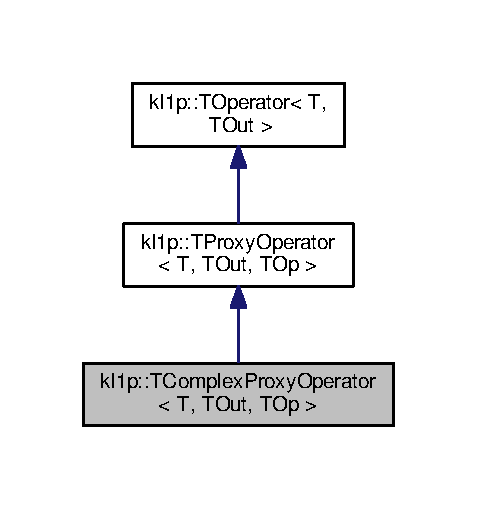
\includegraphics[width=229pt]{classkl1p_1_1TComplexProxyOperator__inherit__graph}
\end{center}
\end{figure}


Collaboration diagram for kl1p\+:\+:T\+Complex\+Proxy\+Operator$<$ T, T\+Out, T\+Op $>$\+:
\nopagebreak
\begin{figure}[H]
\begin{center}
\leavevmode
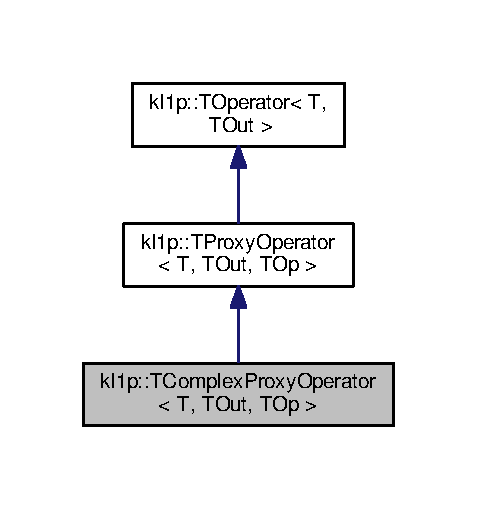
\includegraphics[width=229pt]{classkl1p_1_1TComplexProxyOperator__coll__graph}
\end{center}
\end{figure}
\subsection*{Public Member Functions}
\begin{DoxyCompactItemize}
\item 
{\bfseries T\+Complex\+Proxy\+Operator} (klab\+::\+T\+Smart\+Pointer$<$ T\+Op $>$ op)\hypertarget{classkl1p_1_1TComplexProxyOperator_acaffd59ce065290cbbb7fc93fff217fe}{}\label{classkl1p_1_1TComplexProxyOperator_acaffd59ce065290cbbb7fc93fff217fe}

\item 
{\bfseries T\+Complex\+Proxy\+Operator} (const \hyperlink{classkl1p_1_1TComplexProxyOperator}{T\+Complex\+Proxy\+Operator}$<$ T, T\+Out, T\+Op $>$ \&op)\hypertarget{classkl1p_1_1TComplexProxyOperator_aaea01041d1eb1e5cf3cc6b265414f0b7}{}\label{classkl1p_1_1TComplexProxyOperator_aaea01041d1eb1e5cf3cc6b265414f0b7}

\item 
virtual T {\bfseries sum} ()\hypertarget{classkl1p_1_1TComplexProxyOperator_aee89f4032bb7cc743ccf1a7cbb90f324}{}\label{classkl1p_1_1TComplexProxyOperator_aee89f4032bb7cc743ccf1a7cbb90f324}

\item 
virtual T {\bfseries norm\+Frobenius} ()\hypertarget{classkl1p_1_1TComplexProxyOperator_a3eedda8db25dcbe04a7413a59f0db62f}{}\label{classkl1p_1_1TComplexProxyOperator_a3eedda8db25dcbe04a7413a59f0db62f}

\item 
virtual T {\bfseries squared\+Norm\+Frobenius} ()\hypertarget{classkl1p_1_1TComplexProxyOperator_a3cf9f2e284dec85b0cc4d53ab899ec0e}{}\label{classkl1p_1_1TComplexProxyOperator_a3cf9f2e284dec85b0cc4d53ab899ec0e}

\item 
virtual T {\bfseries mean} ()\hypertarget{classkl1p_1_1TComplexProxyOperator_aa6872789d8901227bfe63e6f28383c4c}{}\label{classkl1p_1_1TComplexProxyOperator_aa6872789d8901227bfe63e6f28383c4c}

\item 
virtual T {\bfseries variance} ()\hypertarget{classkl1p_1_1TComplexProxyOperator_af752e659bb337a1f5e0ffbb69e3a19f5}{}\label{classkl1p_1_1TComplexProxyOperator_af752e659bb337a1f5e0ffbb69e3a19f5}

\item 
virtual void {\bfseries apply} (const arma\+::\+Col$<$ T $>$ \&in, arma\+::\+Col$<$ T\+Out $>$ \&out)\hypertarget{classkl1p_1_1TComplexProxyOperator_a7b98ac54665f284bf3b3936c1ddfbec3}{}\label{classkl1p_1_1TComplexProxyOperator_a7b98ac54665f284bf3b3936c1ddfbec3}

\item 
virtual void {\bfseries apply\+Adjoint} (const arma\+::\+Col$<$ T\+Out $>$ \&in, arma\+::\+Col$<$ T $>$ \&out)\hypertarget{classkl1p_1_1TComplexProxyOperator_a676edd30945e40b8d7a4e11c54080d73}{}\label{classkl1p_1_1TComplexProxyOperator_a676edd30945e40b8d7a4e11c54080d73}

\item 
virtual void {\bfseries column} (klab\+::\+U\+Int32 i, arma\+::\+Col$<$ T\+Out $>$ \&out)\hypertarget{classkl1p_1_1TComplexProxyOperator_a6da69fc2c467496b2a567682ca1bbe0c}{}\label{classkl1p_1_1TComplexProxyOperator_a6da69fc2c467496b2a567682ca1bbe0c}

\item 
virtual void {\bfseries column\+Adjoint} (klab\+::\+U\+Int32 i, arma\+::\+Col$<$ T $>$ \&out)\hypertarget{classkl1p_1_1TComplexProxyOperator_a30c8377005770632f51ff8f45569c030}{}\label{classkl1p_1_1TComplexProxyOperator_a30c8377005770632f51ff8f45569c030}

\end{DoxyCompactItemize}
\subsection*{Additional Inherited Members}


The documentation for this class was generated from the following file\+:\begin{DoxyCompactItemize}
\item 
include/Complex\+Proxy\+Operator.\+h\end{DoxyCompactItemize}

\hypertarget{classkl1p_1_1TCoSaMPHistoryElement}{}\section{kl1p\+:\+:T\+Co\+Sa\+M\+P\+History\+Element$<$ T $>$ Class Template Reference}
\label{classkl1p_1_1TCoSaMPHistoryElement}\index{kl1p\+::\+T\+Co\+Sa\+M\+P\+History\+Element$<$ T $>$@{kl1p\+::\+T\+Co\+Sa\+M\+P\+History\+Element$<$ T $>$}}
\subsection*{Public Member Functions}
\begin{DoxyCompactItemize}
\item 
{\bfseries T\+Co\+Sa\+M\+P\+History\+Element} (const T \&residual\+Norm)\hypertarget{classkl1p_1_1TCoSaMPHistoryElement_a82366484f6c6a943213bfe878da748f3}{}\label{classkl1p_1_1TCoSaMPHistoryElement_a82366484f6c6a943213bfe878da748f3}

\item 
{\bfseries T\+Co\+Sa\+M\+P\+History\+Element} (const \hyperlink{classkl1p_1_1TCoSaMPHistoryElement}{T\+Co\+Sa\+M\+P\+History\+Element}$<$ T $>$ \&element)\hypertarget{classkl1p_1_1TCoSaMPHistoryElement_a7029a151ac5097f65f756a86eed54929}{}\label{classkl1p_1_1TCoSaMPHistoryElement_a7029a151ac5097f65f756a86eed54929}

\item 
\hyperlink{classkl1p_1_1TCoSaMPHistoryElement}{T\+Co\+Sa\+M\+P\+History\+Element}$<$ T $>$ \& {\bfseries operator=} (const \hyperlink{classkl1p_1_1TCoSaMPHistoryElement}{T\+Co\+Sa\+M\+P\+History\+Element}$<$ T $>$ \&element)\hypertarget{classkl1p_1_1TCoSaMPHistoryElement_a305a8fd870b2542304f00170c56229fc}{}\label{classkl1p_1_1TCoSaMPHistoryElement_a305a8fd870b2542304f00170c56229fc}

\item 
const T \& {\bfseries residual\+Norm} () const \hypertarget{classkl1p_1_1TCoSaMPHistoryElement_ab8f779cc6a8a76401db476d849b49a61}{}\label{classkl1p_1_1TCoSaMPHistoryElement_ab8f779cc6a8a76401db476d849b49a61}

\end{DoxyCompactItemize}


The documentation for this class was generated from the following file\+:\begin{DoxyCompactItemize}
\item 
include/Co\+Sa\+M\+P\+History\+Element.\+h\end{DoxyCompactItemize}

\hypertarget{classkl1p_1_1TCoSaMPSolver}{}\section{kl1p\+:\+:T\+Co\+Sa\+M\+P\+Solver$<$ T, T\+Col, T\+Op $>$ Class Template Reference}
\label{classkl1p_1_1TCoSaMPSolver}\index{kl1p\+::\+T\+Co\+Sa\+M\+P\+Solver$<$ T, T\+Col, T\+Op $>$@{kl1p\+::\+T\+Co\+Sa\+M\+P\+Solver$<$ T, T\+Col, T\+Op $>$}}
\subsection*{Public Member Functions}
\begin{DoxyCompactItemize}
\item 
{\bfseries T\+Co\+Sa\+M\+P\+Solver} (const T \&tolerance)\hypertarget{classkl1p_1_1TCoSaMPSolver_a96348b5e1705e769b89ff597cc3cad1a}{}\label{classkl1p_1_1TCoSaMPSolver_a96348b5e1705e769b89ff597cc3cad1a}

\item 
{\bfseries T\+Co\+Sa\+M\+P\+Solver} (const T \&tolerance, klab\+::\+U\+Int32 iteration\+Limit)\hypertarget{classkl1p_1_1TCoSaMPSolver_a8dea5f283ce6621aefbea6cb2098d2ab}{}\label{classkl1p_1_1TCoSaMPSolver_a8dea5f283ce6621aefbea6cb2098d2ab}

\item 
{\bfseries T\+Co\+Sa\+M\+P\+Solver} (const \hyperlink{classkl1p_1_1TCoSaMPSolver}{T\+Co\+Sa\+M\+P\+Solver}$<$ T, T\+Col, T\+Op $>$ \&solver)\hypertarget{classkl1p_1_1TCoSaMPSolver_a7b233b7ef70677ded371e086e412062b}{}\label{classkl1p_1_1TCoSaMPSolver_a7b233b7ef70677ded371e086e412062b}

\item 
\hyperlink{classkl1p_1_1TCoSaMPSolver}{T\+Co\+Sa\+M\+P\+Solver}$<$ T, T\+Col, T\+Op $>$ \& {\bfseries operator=} (const \hyperlink{classkl1p_1_1TCoSaMPSolver}{T\+Co\+Sa\+M\+P\+Solver}$<$ T, T\+Col, T\+Op $>$ \&solver)\hypertarget{classkl1p_1_1TCoSaMPSolver_aa14d917f7f5b58cf4ce5593b5e9ea878}{}\label{classkl1p_1_1TCoSaMPSolver_aa14d917f7f5b58cf4ce5593b5e9ea878}

\item 
void {\bfseries set\+Tolerance} (const T \&tolerance)\hypertarget{classkl1p_1_1TCoSaMPSolver_a2cdebf94c66ff131e2618d2b3a1a0cc1}{}\label{classkl1p_1_1TCoSaMPSolver_a2cdebf94c66ff131e2618d2b3a1a0cc1}

\item 
void {\bfseries set\+Iteration\+Limit} (klab\+::\+U\+Int32 iteration\+Limit)\hypertarget{classkl1p_1_1TCoSaMPSolver_ab83a99eb5ad90197b0398584a080340a}{}\label{classkl1p_1_1TCoSaMPSolver_ab83a99eb5ad90197b0398584a080340a}

\item 
const T \& {\bfseries tolerance} () const \hypertarget{classkl1p_1_1TCoSaMPSolver_aeaf202d939eb1f586ed4c898f817a598}{}\label{classkl1p_1_1TCoSaMPSolver_aeaf202d939eb1f586ed4c898f817a598}

\item 
klab\+::\+U\+Int32 {\bfseries iteration\+Limit} () const \hypertarget{classkl1p_1_1TCoSaMPSolver_a155f17114e2d23c7f529a468d4750b40}{}\label{classkl1p_1_1TCoSaMPSolver_a155f17114e2d23c7f529a468d4750b40}

\item 
const T \& {\bfseries residual\+Norm} () const \hypertarget{classkl1p_1_1TCoSaMPSolver_a3267332ec4a6a4ec560998b7739194d1}{}\label{classkl1p_1_1TCoSaMPSolver_a3267332ec4a6a4ec560998b7739194d1}

\item 
const T \& {\bfseries relative\+Residual\+Norm} () const \hypertarget{classkl1p_1_1TCoSaMPSolver_a4ea2c4972f69dac25dfc1bf0e027a7fd}{}\label{classkl1p_1_1TCoSaMPSolver_a4ea2c4972f69dac25dfc1bf0e027a7fd}

\item 
klab\+::\+U\+Int32 {\bfseries iterations} () const \hypertarget{classkl1p_1_1TCoSaMPSolver_ac288ac8b21a7c70fefe5b0b558fa2cac}{}\label{classkl1p_1_1TCoSaMPSolver_ac288ac8b21a7c70fefe5b0b558fa2cac}

\item 
const klab\+::\+T\+Least\+Square\+System\+Solver$<$ T, T\+Col $>$ \& {\bfseries least\+Square\+Solver} () const \hypertarget{classkl1p_1_1TCoSaMPSolver_a56f0439c7e22237da2be7dae79d78b4a}{}\label{classkl1p_1_1TCoSaMPSolver_a56f0439c7e22237da2be7dae79d78b4a}

\item 
klab\+::\+T\+Least\+Square\+System\+Solver$<$ T, T\+Col $>$ \& {\bfseries least\+Square\+Solver} ()\hypertarget{classkl1p_1_1TCoSaMPSolver_a6d08e0013a95a32370a075b504085bb9}{}\label{classkl1p_1_1TCoSaMPSolver_a6d08e0013a95a32370a075b504085bb9}

\item 
void {\bfseries enable\+History} (bool enable)\hypertarget{classkl1p_1_1TCoSaMPSolver_a48a8165faaf2006a723442fcd57031f9}{}\label{classkl1p_1_1TCoSaMPSolver_a48a8165faaf2006a723442fcd57031f9}

\item 
bool {\bfseries is\+History\+Enabled} () const \hypertarget{classkl1p_1_1TCoSaMPSolver_accbfeef13df767458aadcc1f06a2ce22}{}\label{classkl1p_1_1TCoSaMPSolver_accbfeef13df767458aadcc1f06a2ce22}

\item 
const \hyperlink{classkl1p_1_1THistory}{T\+History}$<$ \hyperlink{classkl1p_1_1TCoSaMPHistoryElement}{T\+Co\+Sa\+M\+P\+History\+Element}$<$ T $>$ $>$ \& {\bfseries history} () const \hypertarget{classkl1p_1_1TCoSaMPSolver_ae63f0b6750a4d2905c4d3a48c35d33e4}{}\label{classkl1p_1_1TCoSaMPSolver_ae63f0b6750a4d2905c4d3a48c35d33e4}

\item 
void {\bfseries solve} (const arma\+::\+Col$<$ T\+Col $>$ \&y, klab\+::\+T\+Smart\+Pointer$<$ T\+Op $>$ phi, klab\+::\+U\+Int32 sparsity, arma\+::\+Col$<$ T\+Col $>$ \&x)\hypertarget{classkl1p_1_1TCoSaMPSolver_aeb947aef9bebf8ce244a9c3b932a20a7}{}\label{classkl1p_1_1TCoSaMPSolver_aeb947aef9bebf8ce244a9c3b932a20a7}

\item 
void {\bfseries solve} (const arma\+::\+Col$<$ T\+Col $>$ \&y, klab\+::\+T\+Smart\+Pointer$<$ T\+Op $>$ phi, klab\+::\+T\+Smart\+Pointer$<$ T\+Op $>$ phiT, klab\+::\+U\+Int32 sparsity, arma\+::\+Col$<$ T\+Col $>$ \&x)\hypertarget{classkl1p_1_1TCoSaMPSolver_afcc889869e6da22c681e5ed06942e851}{}\label{classkl1p_1_1TCoSaMPSolver_afcc889869e6da22c681e5ed06942e851}

\end{DoxyCompactItemize}


The documentation for this class was generated from the following file\+:\begin{DoxyCompactItemize}
\item 
include/Co\+Sa\+M\+P\+Solver.\+h\end{DoxyCompactItemize}

\hypertarget{classkl1p_1_1TDCT1DOperator}{}\section{kl1p\+:\+:T\+D\+C\+T1\+D\+Operator$<$ T $>$ Class Template Reference}
\label{classkl1p_1_1TDCT1DOperator}\index{kl1p\+::\+T\+D\+C\+T1\+D\+Operator$<$ T $>$@{kl1p\+::\+T\+D\+C\+T1\+D\+Operator$<$ T $>$}}


Inheritance diagram for kl1p\+:\+:T\+D\+C\+T1\+D\+Operator$<$ T $>$\+:
\nopagebreak
\begin{figure}[H]
\begin{center}
\leavevmode
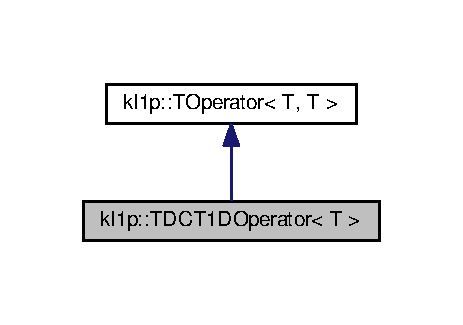
\includegraphics[width=222pt]{classkl1p_1_1TDCT1DOperator__inherit__graph}
\end{center}
\end{figure}


Collaboration diagram for kl1p\+:\+:T\+D\+C\+T1\+D\+Operator$<$ T $>$\+:
\nopagebreak
\begin{figure}[H]
\begin{center}
\leavevmode
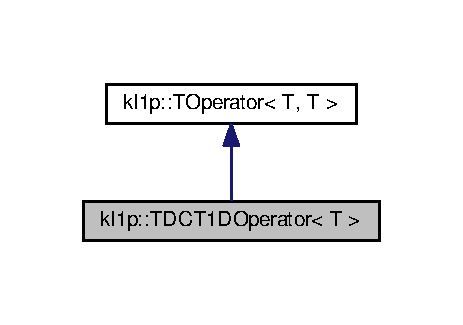
\includegraphics[width=222pt]{classkl1p_1_1TDCT1DOperator__coll__graph}
\end{center}
\end{figure}
\subsection*{Public Member Functions}
\begin{DoxyCompactItemize}
\item 
{\bfseries T\+D\+C\+T1\+D\+Operator} (klab\+::\+U\+Int32 n)\hypertarget{classkl1p_1_1TDCT1DOperator_ac830e532c352e2e3ea24edc5ab34319d}{}\label{classkl1p_1_1TDCT1DOperator_ac830e532c352e2e3ea24edc5ab34319d}

\item 
{\bfseries T\+D\+C\+T1\+D\+Operator} (const \hyperlink{classkl1p_1_1TDCT1DOperator}{T\+D\+C\+T1\+D\+Operator}$<$ T $>$ \&op)\hypertarget{classkl1p_1_1TDCT1DOperator_a0418ee1de32bb7c2160988550cea6dd6}{}\label{classkl1p_1_1TDCT1DOperator_a0418ee1de32bb7c2160988550cea6dd6}

\item 
virtual void {\bfseries apply} (const arma\+::\+Col$<$ T $>$ \&in, arma\+::\+Col$<$ T $>$ \&out)\hypertarget{classkl1p_1_1TDCT1DOperator_af64738f97bed610847054820e18d7900}{}\label{classkl1p_1_1TDCT1DOperator_af64738f97bed610847054820e18d7900}

\item 
virtual void {\bfseries apply\+Adjoint} (const arma\+::\+Col$<$ T $>$ \&in, arma\+::\+Col$<$ T $>$ \&out)\hypertarget{classkl1p_1_1TDCT1DOperator_ab5ca501b22a7416983c23b501b3e377f}{}\label{classkl1p_1_1TDCT1DOperator_ab5ca501b22a7416983c23b501b3e377f}

\end{DoxyCompactItemize}
\subsection*{Additional Inherited Members}


The documentation for this class was generated from the following file\+:\begin{DoxyCompactItemize}
\item 
include/D\+C\+T1\+D\+Operator.\+h\end{DoxyCompactItemize}

\hypertarget{classkl1p_1_1TDCT2DOperator}{}\section{kl1p\+:\+:T\+D\+C\+T2\+D\+Operator$<$ T $>$ Class Template Reference}
\label{classkl1p_1_1TDCT2DOperator}\index{kl1p\+::\+T\+D\+C\+T2\+D\+Operator$<$ T $>$@{kl1p\+::\+T\+D\+C\+T2\+D\+Operator$<$ T $>$}}


Inheritance diagram for kl1p\+:\+:T\+D\+C\+T2\+D\+Operator$<$ T $>$\+:
\nopagebreak
\begin{figure}[H]
\begin{center}
\leavevmode
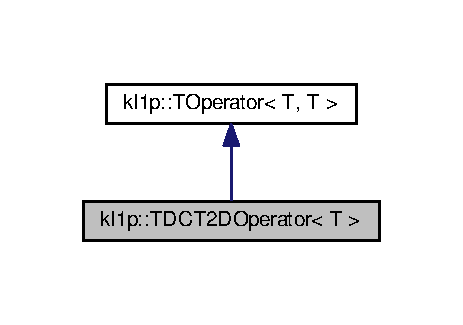
\includegraphics[width=222pt]{classkl1p_1_1TDCT2DOperator__inherit__graph}
\end{center}
\end{figure}


Collaboration diagram for kl1p\+:\+:T\+D\+C\+T2\+D\+Operator$<$ T $>$\+:
\nopagebreak
\begin{figure}[H]
\begin{center}
\leavevmode
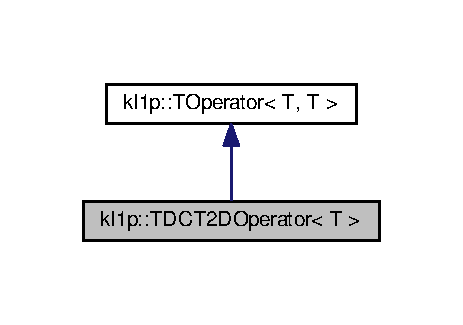
\includegraphics[width=222pt]{classkl1p_1_1TDCT2DOperator__coll__graph}
\end{center}
\end{figure}
\subsection*{Public Member Functions}
\begin{DoxyCompactItemize}
\item 
{\bfseries T\+D\+C\+T2\+D\+Operator} (klab\+::\+U\+Int32 height, klab\+::\+U\+Int32 width)\hypertarget{classkl1p_1_1TDCT2DOperator_a755c0490f848a9cbfac1dae82ae2df1e}{}\label{classkl1p_1_1TDCT2DOperator_a755c0490f848a9cbfac1dae82ae2df1e}

\item 
{\bfseries T\+D\+C\+T2\+D\+Operator} (const \hyperlink{classkl1p_1_1TDCT2DOperator}{T\+D\+C\+T2\+D\+Operator}$<$ T $>$ \&op)\hypertarget{classkl1p_1_1TDCT2DOperator_afc56e77b325b3b9dccc4372c2cd349e3}{}\label{classkl1p_1_1TDCT2DOperator_afc56e77b325b3b9dccc4372c2cd349e3}

\item 
klab\+::\+U\+Int32 {\bfseries width} () const \hypertarget{classkl1p_1_1TDCT2DOperator_ab92aa17505d7be75a6a7c804eb192afa}{}\label{classkl1p_1_1TDCT2DOperator_ab92aa17505d7be75a6a7c804eb192afa}

\item 
klab\+::\+U\+Int32 {\bfseries height} () const \hypertarget{classkl1p_1_1TDCT2DOperator_abf22d3b8de5df8cae3cb0ebcab325613}{}\label{classkl1p_1_1TDCT2DOperator_abf22d3b8de5df8cae3cb0ebcab325613}

\item 
virtual void {\bfseries apply} (const arma\+::\+Col$<$ T $>$ \&in, arma\+::\+Col$<$ T $>$ \&out)\hypertarget{classkl1p_1_1TDCT2DOperator_afdb84577219e4e08176b884bab33ab96}{}\label{classkl1p_1_1TDCT2DOperator_afdb84577219e4e08176b884bab33ab96}

\item 
virtual void {\bfseries apply\+Adjoint} (const arma\+::\+Col$<$ T $>$ \&in, arma\+::\+Col$<$ T $>$ \&out)\hypertarget{classkl1p_1_1TDCT2DOperator_ac61924f3137625ae883514383e5f532e}{}\label{classkl1p_1_1TDCT2DOperator_ac61924f3137625ae883514383e5f532e}

\end{DoxyCompactItemize}
\subsection*{Additional Inherited Members}


The documentation for this class was generated from the following file\+:\begin{DoxyCompactItemize}
\item 
include/D\+C\+T2\+D\+Operator.\+h\end{DoxyCompactItemize}

\hypertarget{classkl1p_1_1TDiagonalOperator}{}\section{kl1p\+:\+:T\+Diagonal\+Operator$<$ T $>$ Class Template Reference}
\label{classkl1p_1_1TDiagonalOperator}\index{kl1p\+::\+T\+Diagonal\+Operator$<$ T $>$@{kl1p\+::\+T\+Diagonal\+Operator$<$ T $>$}}


Inheritance diagram for kl1p\+:\+:T\+Diagonal\+Operator$<$ T $>$\+:
\nopagebreak
\begin{figure}[H]
\begin{center}
\leavevmode
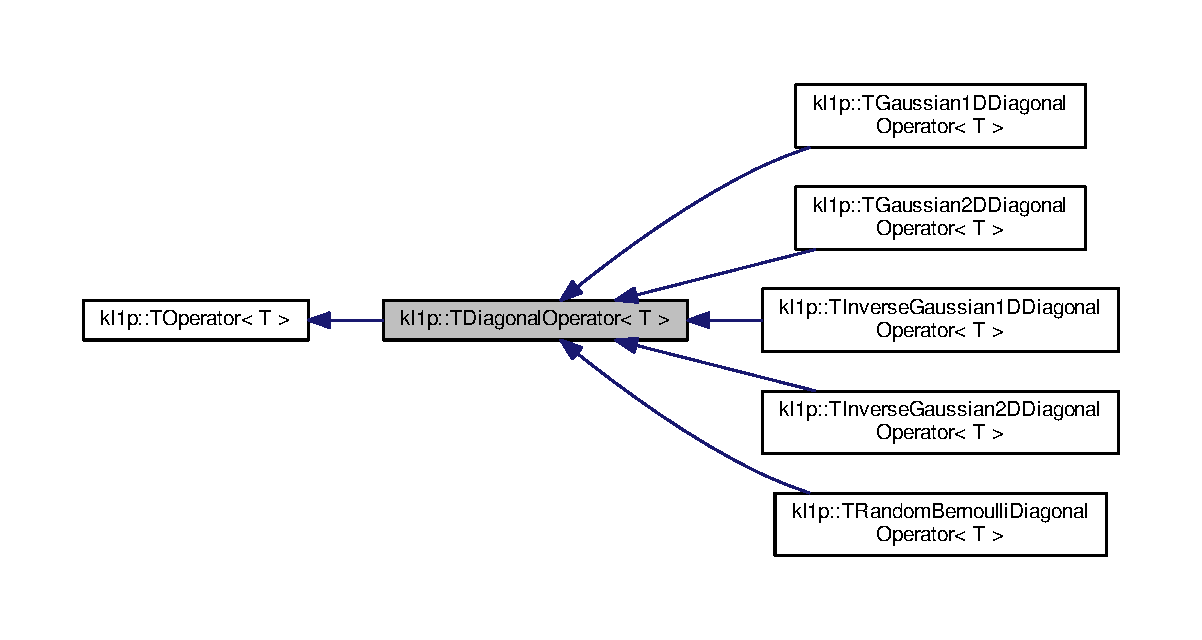
\includegraphics[width=350pt]{classkl1p_1_1TDiagonalOperator__inherit__graph}
\end{center}
\end{figure}


Collaboration diagram for kl1p\+:\+:T\+Diagonal\+Operator$<$ T $>$\+:
\nopagebreak
\begin{figure}[H]
\begin{center}
\leavevmode
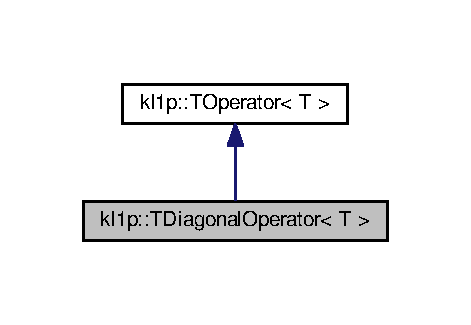
\includegraphics[width=226pt]{classkl1p_1_1TDiagonalOperator__coll__graph}
\end{center}
\end{figure}
\subsection*{Public Member Functions}
\begin{DoxyCompactItemize}
\item 
{\bfseries T\+Diagonal\+Operator} (const arma\+::\+Col$<$ T $>$ \&diag)\hypertarget{classkl1p_1_1TDiagonalOperator_a32e10d270d886d141e27b9df68a4123b}{}\label{classkl1p_1_1TDiagonalOperator_a32e10d270d886d141e27b9df68a4123b}

\item 
{\bfseries T\+Diagonal\+Operator} (const \hyperlink{classkl1p_1_1TDiagonalOperator}{T\+Diagonal\+Operator}$<$ T $>$ \&op)\hypertarget{classkl1p_1_1TDiagonalOperator_a8a3a51ed8ebb2e9084c9a6dd64f79832}{}\label{classkl1p_1_1TDiagonalOperator_a8a3a51ed8ebb2e9084c9a6dd64f79832}

\item 
const arma\+::\+Col$<$ T $>$ \& {\bfseries diagonal} () const \hypertarget{classkl1p_1_1TDiagonalOperator_a8d09ade0b6cea483b619964501c4eaf9}{}\label{classkl1p_1_1TDiagonalOperator_a8d09ade0b6cea483b619964501c4eaf9}

\item 
virtual void {\bfseries apply} (const arma\+::\+Col$<$ T $>$ \&in, arma\+::\+Col$<$ T $>$ \&out)\hypertarget{classkl1p_1_1TDiagonalOperator_aaf78537f9261a1f83fe9942efd2c7fe6}{}\label{classkl1p_1_1TDiagonalOperator_aaf78537f9261a1f83fe9942efd2c7fe6}

\item 
virtual void {\bfseries apply\+Adjoint} (const arma\+::\+Col$<$ T $>$ \&in, arma\+::\+Col$<$ T $>$ \&out)\hypertarget{classkl1p_1_1TDiagonalOperator_a8feb065f8e6f33bfed73a2ae4650f99b}{}\label{classkl1p_1_1TDiagonalOperator_a8feb065f8e6f33bfed73a2ae4650f99b}

\item 
virtual void {\bfseries column} (klab\+::\+U\+Int32 i, arma\+::\+Col$<$ T $>$ \&out)\hypertarget{classkl1p_1_1TDiagonalOperator_a5b79269e3f345fc737023d057c3f4b51}{}\label{classkl1p_1_1TDiagonalOperator_a5b79269e3f345fc737023d057c3f4b51}

\item 
virtual void {\bfseries column\+Adjoint} (klab\+::\+U\+Int32 i, arma\+::\+Col$<$ T $>$ \&out)\hypertarget{classkl1p_1_1TDiagonalOperator_aa30fa6b336e7f44be6eafc1750759c4f}{}\label{classkl1p_1_1TDiagonalOperator_aa30fa6b336e7f44be6eafc1750759c4f}

\end{DoxyCompactItemize}
\subsection*{Protected Member Functions}
\begin{DoxyCompactItemize}
\item 
void {\bfseries set\+Diagonal} (const arma\+::\+Col$<$ T $>$ \&diag)\hypertarget{classkl1p_1_1TDiagonalOperator_a71d5b6147b5b055ba82ee2c69e983d2d}{}\label{classkl1p_1_1TDiagonalOperator_a71d5b6147b5b055ba82ee2c69e983d2d}

\end{DoxyCompactItemize}


The documentation for this class was generated from the following file\+:\begin{DoxyCompactItemize}
\item 
include/Diagonal\+Operator.\+h\end{DoxyCompactItemize}

\hypertarget{classkl1p_1_1TDownSamplingOperator}{}\section{kl1p\+:\+:T\+Down\+Sampling\+Operator$<$ T $>$ Class Template Reference}
\label{classkl1p_1_1TDownSamplingOperator}\index{kl1p\+::\+T\+Down\+Sampling\+Operator$<$ T $>$@{kl1p\+::\+T\+Down\+Sampling\+Operator$<$ T $>$}}


Inheritance diagram for kl1p\+:\+:T\+Down\+Sampling\+Operator$<$ T $>$\+:
\nopagebreak
\begin{figure}[H]
\begin{center}
\leavevmode
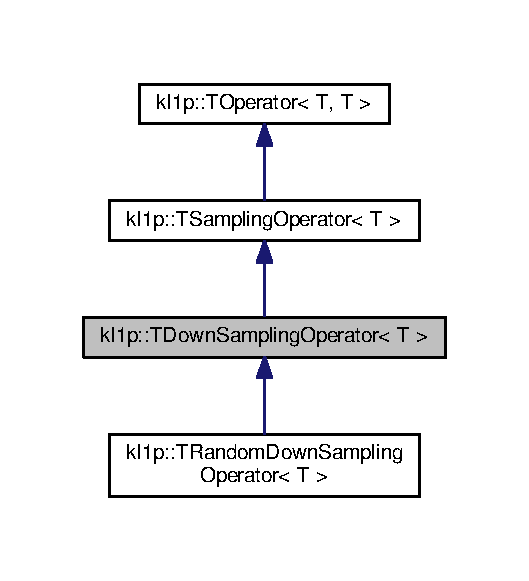
\includegraphics[width=254pt]{classkl1p_1_1TDownSamplingOperator__inherit__graph}
\end{center}
\end{figure}


Collaboration diagram for kl1p\+:\+:T\+Down\+Sampling\+Operator$<$ T $>$\+:
\nopagebreak
\begin{figure}[H]
\begin{center}
\leavevmode
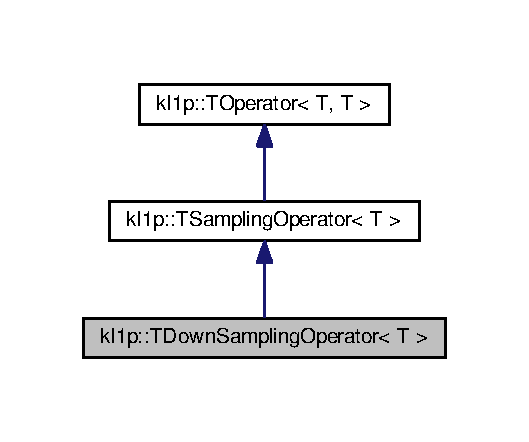
\includegraphics[width=254pt]{classkl1p_1_1TDownSamplingOperator__coll__graph}
\end{center}
\end{figure}
\subsection*{Public Member Functions}
\begin{DoxyCompactItemize}
\item 
{\bfseries T\+Down\+Sampling\+Operator} (klab\+::\+U\+Int32 n, const kl1p\+::\+K\+Sampling\+Indices\+Array \&indices)\hypertarget{classkl1p_1_1TDownSamplingOperator_a0f0e945252682fa278a0379aea74b006}{}\label{classkl1p_1_1TDownSamplingOperator_a0f0e945252682fa278a0379aea74b006}

\item 
{\bfseries T\+Down\+Sampling\+Operator} (const klab\+::\+K\+Bit\+Array \&mask)\hypertarget{classkl1p_1_1TDownSamplingOperator_a46a2f3210bd04cadf18762bc3c5e8f8f}{}\label{classkl1p_1_1TDownSamplingOperator_a46a2f3210bd04cadf18762bc3c5e8f8f}

\item 
{\bfseries T\+Down\+Sampling\+Operator} (const \hyperlink{classkl1p_1_1TDownSamplingOperator}{T\+Down\+Sampling\+Operator}$<$ T $>$ \&op)\hypertarget{classkl1p_1_1TDownSamplingOperator_a65edea2d8799091f64ef90f4cdad455a}{}\label{classkl1p_1_1TDownSamplingOperator_a65edea2d8799091f64ef90f4cdad455a}

\end{DoxyCompactItemize}
\subsection*{Protected Member Functions}
\begin{DoxyCompactItemize}
\item 
void {\bfseries set\+Mask} (const klab\+::\+K\+Bit\+Array \&mask)\hypertarget{classkl1p_1_1TDownSamplingOperator_af4ebe3e7370c1ea995e1130edb577840}{}\label{classkl1p_1_1TDownSamplingOperator_af4ebe3e7370c1ea995e1130edb577840}

\end{DoxyCompactItemize}


The documentation for this class was generated from the following file\+:\begin{DoxyCompactItemize}
\item 
include/Down\+Sampling\+Operator.\+h\end{DoxyCompactItemize}

\hypertarget{classkl1p_1_1TEMBPHistoryElement}{}\section{kl1p\+:\+:T\+E\+M\+B\+P\+History\+Element$<$ T $>$ Class Template Reference}
\label{classkl1p_1_1TEMBPHistoryElement}\index{kl1p\+::\+T\+E\+M\+B\+P\+History\+Element$<$ T $>$@{kl1p\+::\+T\+E\+M\+B\+P\+History\+Element$<$ T $>$}}
\subsection*{Public Member Functions}
\begin{DoxyCompactItemize}
\item 
{\bfseries T\+E\+M\+B\+P\+History\+Element} (const T \&residual\+Norm)\hypertarget{classkl1p_1_1TEMBPHistoryElement_ada9e3887c38f64fb3ef89c05378f91bc}{}\label{classkl1p_1_1TEMBPHistoryElement_ada9e3887c38f64fb3ef89c05378f91bc}

\item 
{\bfseries T\+E\+M\+B\+P\+History\+Element} (const \hyperlink{classkl1p_1_1TEMBPHistoryElement}{T\+E\+M\+B\+P\+History\+Element}$<$ T $>$ \&element)\hypertarget{classkl1p_1_1TEMBPHistoryElement_a01554a366a628c102929c8e264383320}{}\label{classkl1p_1_1TEMBPHistoryElement_a01554a366a628c102929c8e264383320}

\item 
\hyperlink{classkl1p_1_1TEMBPHistoryElement}{T\+E\+M\+B\+P\+History\+Element}$<$ T $>$ \& {\bfseries operator=} (const \hyperlink{classkl1p_1_1TEMBPHistoryElement}{T\+E\+M\+B\+P\+History\+Element}$<$ T $>$ \&element)\hypertarget{classkl1p_1_1TEMBPHistoryElement_ae9c79886fc15aaa86b764db52a04cf68}{}\label{classkl1p_1_1TEMBPHistoryElement_ae9c79886fc15aaa86b764db52a04cf68}

\item 
const T \& {\bfseries residual\+Norm} () const \hypertarget{classkl1p_1_1TEMBPHistoryElement_abda34c2aff6396bb43ff6ef2753cfc34}{}\label{classkl1p_1_1TEMBPHistoryElement_abda34c2aff6396bb43ff6ef2753cfc34}

\end{DoxyCompactItemize}


The documentation for this class was generated from the following file\+:\begin{DoxyCompactItemize}
\item 
include/E\+M\+B\+P\+History\+Element.\+h\end{DoxyCompactItemize}

\hypertarget{classkl1p_1_1TEMBPSolver}{}\section{kl1p\+:\+:T\+E\+M\+B\+P\+Solver$<$ T, T\+Col, T\+Op $>$ Class Template Reference}
\label{classkl1p_1_1TEMBPSolver}\index{kl1p\+::\+T\+E\+M\+B\+P\+Solver$<$ T, T\+Col, T\+Op $>$@{kl1p\+::\+T\+E\+M\+B\+P\+Solver$<$ T, T\+Col, T\+Op $>$}}
\subsection*{Public Member Functions}
\begin{DoxyCompactItemize}
\item 
{\bfseries T\+E\+M\+B\+P\+Solver} (const T \&tolerance)\hypertarget{classkl1p_1_1TEMBPSolver_a856117ea2047cd66894f103bc944d1b3}{}\label{classkl1p_1_1TEMBPSolver_a856117ea2047cd66894f103bc944d1b3}

\item 
{\bfseries T\+E\+M\+B\+P\+Solver} (const T \&tolerance, klab\+::\+U\+Int32 iteration\+Limit)\hypertarget{classkl1p_1_1TEMBPSolver_a0b8ab5ee3a713057bcf31cbe909f7051}{}\label{classkl1p_1_1TEMBPSolver_a0b8ab5ee3a713057bcf31cbe909f7051}

\item 
{\bfseries T\+E\+M\+B\+P\+Solver} (const \hyperlink{classkl1p_1_1TEMBPSolver}{T\+E\+M\+B\+P\+Solver}$<$ T, T\+Col, T\+Op $>$ \&solver)\hypertarget{classkl1p_1_1TEMBPSolver_af88bc940a84ec4f402dd1d4e75426a07}{}\label{classkl1p_1_1TEMBPSolver_af88bc940a84ec4f402dd1d4e75426a07}

\item 
\hyperlink{classkl1p_1_1TEMBPSolver}{T\+E\+M\+B\+P\+Solver}$<$ T, T\+Col, T\+Op $>$ \& {\bfseries operator=} (const \hyperlink{classkl1p_1_1TEMBPSolver}{T\+E\+M\+B\+P\+Solver}$<$ T, T\+Col, T\+Op $>$ \&solver)\hypertarget{classkl1p_1_1TEMBPSolver_a86d10121f5ea67f7270ae9b5968789e2}{}\label{classkl1p_1_1TEMBPSolver_a86d10121f5ea67f7270ae9b5968789e2}

\item 
void {\bfseries set\+Tolerance} (const T \&tolerance)\hypertarget{classkl1p_1_1TEMBPSolver_a8eb376dcd7004e98e11a6c6c2da26210}{}\label{classkl1p_1_1TEMBPSolver_a8eb376dcd7004e98e11a6c6c2da26210}

\item 
void {\bfseries set\+Iteration\+Limit} (klab\+::\+U\+Int32 iteration\+Limit)\hypertarget{classkl1p_1_1TEMBPSolver_a646a17e2d77557d905efeec9b3107a20}{}\label{classkl1p_1_1TEMBPSolver_a646a17e2d77557d905efeec9b3107a20}

\item 
void {\bfseries set\+Noise\+Variance} (const T \&noise)\hypertarget{classkl1p_1_1TEMBPSolver_af62b389f6722883a4c50e77e4691f54b}{}\label{classkl1p_1_1TEMBPSolver_af62b389f6722883a4c50e77e4691f54b}

\item 
void {\bfseries set\+Message\+Damping} (const T \&damping)\hypertarget{classkl1p_1_1TEMBPSolver_a305cd56334caefb0119ac46d81494ecc}{}\label{classkl1p_1_1TEMBPSolver_a305cd56334caefb0119ac46d81494ecc}

\item 
void {\bfseries set\+Learning\+Damping} (const T \&damping)\hypertarget{classkl1p_1_1TEMBPSolver_a3ed2ed7b5f64b3469b2c76c0129aec05}{}\label{classkl1p_1_1TEMBPSolver_a3ed2ed7b5f64b3469b2c76c0129aec05}

\item 
void {\bfseries enable\+Damping\+Learning} (bool enable)\hypertarget{classkl1p_1_1TEMBPSolver_a2943dbc17a474ec05336cfac88d02fda}{}\label{classkl1p_1_1TEMBPSolver_a2943dbc17a474ec05336cfac88d02fda}

\item 
void {\bfseries enable\+Parameter\+Learning} (bool enable)\hypertarget{classkl1p_1_1TEMBPSolver_a3a1a8dfa6262c60276d6fbdf49634480}{}\label{classkl1p_1_1TEMBPSolver_a3a1a8dfa6262c60276d6fbdf49634480}

\item 
void {\bfseries enable\+Homogeneous} (bool enable)\hypertarget{classkl1p_1_1TEMBPSolver_ad7693a301d0a6079a9150ed82352ec64}{}\label{classkl1p_1_1TEMBPSolver_ad7693a301d0a6079a9150ed82352ec64}

\item 
const T \& {\bfseries tolerance} () const \hypertarget{classkl1p_1_1TEMBPSolver_afc6bf6a1c0a0bda420705f3777df8156}{}\label{classkl1p_1_1TEMBPSolver_afc6bf6a1c0a0bda420705f3777df8156}

\item 
klab\+::\+U\+Int32 {\bfseries iteration\+Limit} () const \hypertarget{classkl1p_1_1TEMBPSolver_aa310ef9f0fd27b73d9bc2ccd78e83faf}{}\label{classkl1p_1_1TEMBPSolver_aa310ef9f0fd27b73d9bc2ccd78e83faf}

\item 
const T \& {\bfseries noise\+Variance} () const \hypertarget{classkl1p_1_1TEMBPSolver_a5c8ba3811fd115c8a6ca1f608118a3fb}{}\label{classkl1p_1_1TEMBPSolver_a5c8ba3811fd115c8a6ca1f608118a3fb}

\item 
const T \& {\bfseries message\+Damping} () const \hypertarget{classkl1p_1_1TEMBPSolver_a088e1674c71dfca92e068336cb44fa9d}{}\label{classkl1p_1_1TEMBPSolver_a088e1674c71dfca92e068336cb44fa9d}

\item 
const T \& {\bfseries learning\+Damping} () const \hypertarget{classkl1p_1_1TEMBPSolver_a09a6951ad3608a87b959c22648a92e0f}{}\label{classkl1p_1_1TEMBPSolver_a09a6951ad3608a87b959c22648a92e0f}

\item 
bool {\bfseries is\+Damping\+Learning\+Enabled} () const \hypertarget{classkl1p_1_1TEMBPSolver_a3303dcbc341c1e89f6e95ca9d33903bc}{}\label{classkl1p_1_1TEMBPSolver_a3303dcbc341c1e89f6e95ca9d33903bc}

\item 
bool {\bfseries is\+Parameter\+Learning\+Enabled} () const \hypertarget{classkl1p_1_1TEMBPSolver_a5f9366a2a615867fdd565bdccdcf8cad}{}\label{classkl1p_1_1TEMBPSolver_a5f9366a2a615867fdd565bdccdcf8cad}

\item 
bool {\bfseries is\+Homogeneous\+Enabled} () const \hypertarget{classkl1p_1_1TEMBPSolver_a2dbd29bfa856b783efc610f6a7bd73d1}{}\label{classkl1p_1_1TEMBPSolver_a2dbd29bfa856b783efc610f6a7bd73d1}

\item 
const T \& {\bfseries residual\+Norm} () const \hypertarget{classkl1p_1_1TEMBPSolver_aab34ff0b4faa97da804f1cc18cced983}{}\label{classkl1p_1_1TEMBPSolver_aab34ff0b4faa97da804f1cc18cced983}

\item 
const T \& {\bfseries relative\+Residual\+Norm} () const \hypertarget{classkl1p_1_1TEMBPSolver_ab91e651a140f12f480b7f4875065ccbf}{}\label{classkl1p_1_1TEMBPSolver_ab91e651a140f12f480b7f4875065ccbf}

\item 
klab\+::\+U\+Int32 {\bfseries iterations} () const \hypertarget{classkl1p_1_1TEMBPSolver_a8bd02ae1f6d0c6b3a64ad9072c57f3f3}{}\label{classkl1p_1_1TEMBPSolver_a8bd02ae1f6d0c6b3a64ad9072c57f3f3}

\item 
void {\bfseries enable\+History} (bool enable)\hypertarget{classkl1p_1_1TEMBPSolver_a9f18525ea90d95b2cd18abf8c1d2d35f}{}\label{classkl1p_1_1TEMBPSolver_a9f18525ea90d95b2cd18abf8c1d2d35f}

\item 
bool {\bfseries is\+History\+Enabled} () const \hypertarget{classkl1p_1_1TEMBPSolver_a3587704719ae3e128443cb1211826765}{}\label{classkl1p_1_1TEMBPSolver_a3587704719ae3e128443cb1211826765}

\item 
const \hyperlink{classkl1p_1_1THistory}{T\+History}$<$ \hyperlink{classkl1p_1_1TEMBPHistoryElement}{T\+E\+M\+B\+P\+History\+Element}$<$ T $>$ $>$ \& {\bfseries history} () const \hypertarget{classkl1p_1_1TEMBPSolver_a5c636072b19779ddd69df4f24ff53413}{}\label{classkl1p_1_1TEMBPSolver_a5c636072b19779ddd69df4f24ff53413}

\item 
void {\bfseries solve} (const arma\+::\+Col$<$ T\+Col $>$ \&y, klab\+::\+T\+Smart\+Pointer$<$ T\+Op $>$ phi, klab\+::\+U\+Int32 sparsity, arma\+::\+Col$<$ T\+Col $>$ \&x)\hypertarget{classkl1p_1_1TEMBPSolver_af62313de80c147133450a29b1f84d548}{}\label{classkl1p_1_1TEMBPSolver_af62313de80c147133450a29b1f84d548}

\item 
void {\bfseries solve} (const arma\+::\+Col$<$ T\+Col $>$ \&y, klab\+::\+T\+Smart\+Pointer$<$ T\+Op $>$ phi, klab\+::\+T\+Smart\+Pointer$<$ T\+Op $>$ phiT, klab\+::\+U\+Int32 sparsity, arma\+::\+Col$<$ T\+Col $>$ \&x)\hypertarget{classkl1p_1_1TEMBPSolver_a5917cc22bb0d363f8a74746c2914f1a5}{}\label{classkl1p_1_1TEMBPSolver_a5917cc22bb0d363f8a74746c2914f1a5}

\item 
void {\bfseries solve} (const arma\+::\+Col$<$ T\+Col $>$ \&y, klab\+::\+T\+Smart\+Pointer$<$ \hyperlink{classkl1p_1_1TBlockOperator}{T\+Block\+Operator}$<$ T\+Col, T\+Col, T\+Op $>$ $>$ phi, klab\+::\+U\+Int32 sparsity, arma\+::\+Col$<$ T\+Col $>$ \&x)\hypertarget{classkl1p_1_1TEMBPSolver_ad459dd049e4673686094fd3f0adff719}{}\label{classkl1p_1_1TEMBPSolver_ad459dd049e4673686094fd3f0adff719}

\item 
void {\bfseries solve} (const arma\+::\+Col$<$ T\+Col $>$ \&y, klab\+::\+T\+Smart\+Pointer$<$ \hyperlink{classkl1p_1_1TBlockOperator}{T\+Block\+Operator}$<$ T\+Col, T\+Col, T\+Op $>$ $>$ phi, klab\+::\+T\+Smart\+Pointer$<$ \hyperlink{classkl1p_1_1TBlockOperator}{T\+Block\+Operator}$<$ T\+Col, T\+Col, T\+Op $>$ $>$ phiT, klab\+::\+U\+Int32 sparsity, arma\+::\+Col$<$ T\+Col $>$ \&x)\hypertarget{classkl1p_1_1TEMBPSolver_a126d313f3a018fbcd3e8ce4dd449eb89}{}\label{classkl1p_1_1TEMBPSolver_a126d313f3a018fbcd3e8ce4dd449eb89}

\end{DoxyCompactItemize}
\subsection*{Protected Member Functions}
\begin{DoxyCompactItemize}
\item 
void {\bfseries solve\+E\+M\+BP} (const arma\+::\+Col$<$ T\+Col $>$ \&y, klab\+::\+T\+Smart\+Pointer$<$ T\+Op $>$ phi, klab\+::\+T\+Smart\+Pointer$<$ T\+Op $>$ phiT, klab\+::\+U\+Int32 sparsity, arma\+::\+Col$<$ T\+Col $>$ \&x, T \&residual\+Norm, T \&relative\+Residual\+Norm, klab\+::\+U\+Int32 \&iterations, \hyperlink{classkl1p_1_1THistory}{T\+History}$<$ \hyperlink{classkl1p_1_1TEMBPHistoryElement}{T\+E\+M\+B\+P\+History\+Element}$<$ T $>$ $>$ \&history)\hypertarget{classkl1p_1_1TEMBPSolver_a47d227e9eda5cca46bd5c8539aa6547f}{}\label{classkl1p_1_1TEMBPSolver_a47d227e9eda5cca46bd5c8539aa6547f}

\item 
void {\bfseries solve\+E\+M\+BP} (const arma\+::\+Col$<$ T\+Col $>$ \&y, klab\+::\+T\+Smart\+Pointer$<$ \hyperlink{classkl1p_1_1TBlockOperator}{T\+Block\+Operator}$<$ T\+Col, T\+Col, T\+Op $>$ $>$ phi, klab\+::\+T\+Smart\+Pointer$<$ \hyperlink{classkl1p_1_1TBlockOperator}{T\+Block\+Operator}$<$ T\+Col, T\+Col, T\+Op $>$ $>$ phiT, klab\+::\+U\+Int32 sparsity, arma\+::\+Col$<$ T\+Col $>$ \&x, T \&residual\+Norm, T \&relative\+Residual\+Norm, klab\+::\+U\+Int32 \&iterations, \hyperlink{classkl1p_1_1THistory}{T\+History}$<$ \hyperlink{classkl1p_1_1TEMBPHistoryElement}{T\+E\+M\+B\+P\+History\+Element}$<$ T $>$ $>$ \&history)\hypertarget{classkl1p_1_1TEMBPSolver_a78f4dd58130e5ce14e4e732b6b2e2f90}{}\label{classkl1p_1_1TEMBPSolver_a78f4dd58130e5ce14e4e732b6b2e2f90}

\item 
void {\bfseries solve\+E\+M\+B\+P\+\_\+\+Homogeneous} (const arma\+::\+Col$<$ T\+Col $>$ \&y, klab\+::\+T\+Smart\+Pointer$<$ T\+Op $>$ phi, klab\+::\+T\+Smart\+Pointer$<$ T\+Op $>$ phiT, klab\+::\+U\+Int32 sparsity, arma\+::\+Col$<$ T\+Col $>$ \&x, T \&residual\+Norm, T \&relative\+Residual\+Norm, klab\+::\+U\+Int32 \&iterations, \hyperlink{classkl1p_1_1THistory}{T\+History}$<$ \hyperlink{classkl1p_1_1TEMBPHistoryElement}{T\+E\+M\+B\+P\+History\+Element}$<$ T $>$ $>$ \&history)\hypertarget{classkl1p_1_1TEMBPSolver_a10338258f5776caa83cfda65f908d00d}{}\label{classkl1p_1_1TEMBPSolver_a10338258f5776caa83cfda65f908d00d}

\item 
void {\bfseries solve\+E\+M\+B\+P\+\_\+\+Generic} (const arma\+::\+Col$<$ T\+Col $>$ \&y, klab\+::\+T\+Smart\+Pointer$<$ T\+Op $>$ phi, klab\+::\+T\+Smart\+Pointer$<$ T\+Op $>$ phiT, klab\+::\+U\+Int32 sparsity, arma\+::\+Col$<$ T\+Col $>$ \&x, T \&residual\+Norm, T \&relative\+Residual\+Norm, klab\+::\+U\+Int32 \&iterations, \hyperlink{classkl1p_1_1THistory}{T\+History}$<$ \hyperlink{classkl1p_1_1TEMBPHistoryElement}{T\+E\+M\+B\+P\+History\+Element}$<$ T $>$ $>$ \&history)\hypertarget{classkl1p_1_1TEMBPSolver_ac74440d0d069be695d06eec08b860578}{}\label{classkl1p_1_1TEMBPSolver_ac74440d0d069be695d06eec08b860578}

\end{DoxyCompactItemize}
\subsection*{Static Protected Member Functions}
\begin{DoxyCompactItemize}
\item 
static void {\bfseries Compute\+Fa\+\_\+\+Homogeneous} (const T\+Col \&u, const arma\+::\+Col$<$ T\+Col $>$ \&v, const T\+Col \&rho, const T\+Col \&mean, const T\+Col \&sigma, arma\+::\+Col$<$ T\+Col $>$ \&out)\hypertarget{classkl1p_1_1TEMBPSolver_a24d9c943b040924be1414fb50d364595}{}\label{classkl1p_1_1TEMBPSolver_a24d9c943b040924be1414fb50d364595}

\item 
static void {\bfseries Compute\+Fb\+\_\+\+Homogeneous} (const T\+Col \&u, const arma\+::\+Col$<$ T\+Col $>$ \&v, const T\+Col \&rho, const T\+Col \&mean, const T\+Col \&sigma, arma\+::\+Col$<$ T\+Col $>$ \&out)\hypertarget{classkl1p_1_1TEMBPSolver_aeead007c79872bfd7cd4d0455cf84692}{}\label{classkl1p_1_1TEMBPSolver_aeead007c79872bfd7cd4d0455cf84692}

\item 
static T\+Col {\bfseries Compute\+Rho\+Learning\+\_\+\+Homogeneous} (const T\+Col \&rho, const T\+Col \&u, const arma\+::\+Col$<$ T\+Col $>$ \&v, const arma\+::\+Col$<$ T\+Col $>$ \&fa, const T\+Col \&alpha, const T\+Col \&mean, const T\+Col \&sigma)\hypertarget{classkl1p_1_1TEMBPSolver_a12bc80a9268a440edc0d4603734bb898}{}\label{classkl1p_1_1TEMBPSolver_a12bc80a9268a440edc0d4603734bb898}

\item 
static T\+Col {\bfseries Compute\+Noise\+Learning\+\_\+\+Homogeneous} (const T\+Col \&noise, const arma\+::\+Col$<$ T\+Col $>$ \&y, const arma\+::\+Col$<$ T\+Col $>$ \&w, const T\+Col \&gamma)\hypertarget{classkl1p_1_1TEMBPSolver_a97e92cc9ca1d75cdf74b6c068214eaf8}{}\label{classkl1p_1_1TEMBPSolver_a97e92cc9ca1d75cdf74b6c068214eaf8}

\item 
static void {\bfseries Compute\+Fa\+\_\+\+Generic} (const arma\+::\+Col$<$ T\+Col $>$ \&u, const arma\+::\+Col$<$ T\+Col $>$ \&v, const T\+Col \&rho, const T\+Col \&mean, const T\+Col \&sigma, arma\+::\+Col$<$ T\+Col $>$ \&out)\hypertarget{classkl1p_1_1TEMBPSolver_a7813216d7a86086ba2b72e65ea30a76b}{}\label{classkl1p_1_1TEMBPSolver_a7813216d7a86086ba2b72e65ea30a76b}

\item 
static void {\bfseries Compute\+Fb\+\_\+\+Generic} (const arma\+::\+Col$<$ T\+Col $>$ \&u, const arma\+::\+Col$<$ T\+Col $>$ \&v, const T\+Col \&rho, const T\+Col \&mean, const T\+Col \&sigma, arma\+::\+Col$<$ T\+Col $>$ \&out)\hypertarget{classkl1p_1_1TEMBPSolver_a9e73a54e8d8e23585b97360469e6d425}{}\label{classkl1p_1_1TEMBPSolver_a9e73a54e8d8e23585b97360469e6d425}

\item 
static T\+Col {\bfseries Compute\+Rho\+Learning\+\_\+\+Generic} (const T\+Col \&rho, const arma\+::\+Col$<$ T\+Col $>$ \&u, const arma\+::\+Col$<$ T\+Col $>$ \&v, const arma\+::\+Col$<$ T\+Col $>$ \&fa, const T\+Col \&alpha, const T\+Col \&mean, const T\+Col \&sigma)\hypertarget{classkl1p_1_1TEMBPSolver_ad9b717cd1af082b4d8f950b48f24b330}{}\label{classkl1p_1_1TEMBPSolver_ad9b717cd1af082b4d8f950b48f24b330}

\item 
static T\+Col {\bfseries Compute\+Noise\+Learning\+\_\+\+Generic} (const T\+Col \&noise, const arma\+::\+Col$<$ T\+Col $>$ \&y, const arma\+::\+Col$<$ T\+Col $>$ \&w, const arma\+::\+Col$<$ T\+Col $>$ \&gamma)\hypertarget{classkl1p_1_1TEMBPSolver_a03cb2c068df45df3cd69e5b0dcb74c20}{}\label{classkl1p_1_1TEMBPSolver_a03cb2c068df45df3cd69e5b0dcb74c20}

\item 
static void {\bfseries Compute\+Damping} (const arma\+::\+Col$<$ T\+Col $>$ \&u, const arma\+::\+Col$<$ T\+Col $>$ \&v, const T\+Col \&damp, arma\+::\+Col$<$ T\+Col $>$ \&out)\hypertarget{classkl1p_1_1TEMBPSolver_ab87a0fbcbb23bde5ffcc14dc0dec1de6}{}\label{classkl1p_1_1TEMBPSolver_ab87a0fbcbb23bde5ffcc14dc0dec1de6}

\item 
static T\+Col {\bfseries Compute\+Mean\+Learning} (const arma\+::\+Col$<$ T\+Col $>$ \&fa, const T\+Col \&rho)\hypertarget{classkl1p_1_1TEMBPSolver_ae05e150ae80c6c53a5d2564437a6d117}{}\label{classkl1p_1_1TEMBPSolver_ae05e150ae80c6c53a5d2564437a6d117}

\item 
static T\+Col {\bfseries Compute\+Sigma\+Learning} (const arma\+::\+Col$<$ T\+Col $>$ \&fa, const arma\+::\+Col$<$ T\+Col $>$ \&fb, const T\+Col \&rho, const T\+Col \&mean)\hypertarget{classkl1p_1_1TEMBPSolver_a80e62edf7a1269d87b72287f1bcf4e7f}{}\label{classkl1p_1_1TEMBPSolver_a80e62edf7a1269d87b72287f1bcf4e7f}

\item 
static T\+Col {\bfseries Compute\+Variance\+Learning} (const arma\+::\+Col$<$ T\+Col $>$ \&fa, const arma\+::\+Col$<$ T\+Col $>$ \&fb, const T\+Col \&rho)\hypertarget{classkl1p_1_1TEMBPSolver_ad8b0cb460720ab7a7e3de14f54ad7d10}{}\label{classkl1p_1_1TEMBPSolver_ad8b0cb460720ab7a7e3de14f54ad7d10}

\end{DoxyCompactItemize}
\subsection*{Friends}
\begin{DoxyCompactItemize}
\item 
{\footnotesize template$<$class U , class U\+Col , class U\+Op $>$ }\\class {\bfseries T\+E\+M\+B\+P\+Solver\+Specialisation}\hypertarget{classkl1p_1_1TEMBPSolver_a2158ad5bc07c5e0e2adefae8c0b21ffb}{}\label{classkl1p_1_1TEMBPSolver_a2158ad5bc07c5e0e2adefae8c0b21ffb}

\end{DoxyCompactItemize}


The documentation for this class was generated from the following file\+:\begin{DoxyCompactItemize}
\item 
include/E\+M\+B\+P\+Solver.\+h\end{DoxyCompactItemize}

\hypertarget{classkl1p_1_1TEMBPSolverSpecialisation}{}\section{kl1p\+:\+:T\+E\+M\+B\+P\+Solver\+Specialisation$<$ T, T\+Col, T\+Op $>$ Class Template Reference}
\label{classkl1p_1_1TEMBPSolverSpecialisation}\index{kl1p\+::\+T\+E\+M\+B\+P\+Solver\+Specialisation$<$ T, T\+Col, T\+Op $>$@{kl1p\+::\+T\+E\+M\+B\+P\+Solver\+Specialisation$<$ T, T\+Col, T\+Op $>$}}
\subsection*{Static Public Member Functions}
\begin{DoxyCompactItemize}
\item 
static void {\bfseries Solve} (const arma\+::\+Col$<$ T\+Col $>$ \&y, klab\+::\+T\+Smart\+Pointer$<$ T\+Op $>$ phi, klab\+::\+T\+Smart\+Pointer$<$ T\+Op $>$ phiT, klab\+::\+U\+Int32 sparsity, arma\+::\+Col$<$ T\+Col $>$ \&x, \hyperlink{classkl1p_1_1TEMBPSolver}{T\+E\+M\+B\+P\+Solver}$<$ T, T\+Col, T\+Op $>$ \&solver)\hypertarget{classkl1p_1_1TEMBPSolverSpecialisation_adfb7b0d38e9e7d5cf07189089314e9a0}{}\label{classkl1p_1_1TEMBPSolverSpecialisation_adfb7b0d38e9e7d5cf07189089314e9a0}

\item 
static void {\bfseries Solve} (const arma\+::\+Col$<$ T\+Col $>$ \&y, klab\+::\+T\+Smart\+Pointer$<$ \hyperlink{classkl1p_1_1TBlockOperator}{T\+Block\+Operator}$<$ T\+Col, T\+Col, T\+Op $>$ $>$ phi, klab\+::\+T\+Smart\+Pointer$<$ \hyperlink{classkl1p_1_1TBlockOperator}{T\+Block\+Operator}$<$ T\+Col, T\+Col, T\+Op $>$ $>$ phiT, klab\+::\+U\+Int32 sparsity, arma\+::\+Col$<$ T\+Col $>$ \&x, \hyperlink{classkl1p_1_1TEMBPSolver}{T\+E\+M\+B\+P\+Solver}$<$ T, T\+Col, T\+Op $>$ \&solver)\hypertarget{classkl1p_1_1TEMBPSolverSpecialisation_a92521c0535fbe6ae449cfb9e7e9fa0ab}{}\label{classkl1p_1_1TEMBPSolverSpecialisation_a92521c0535fbe6ae449cfb9e7e9fa0ab}

\end{DoxyCompactItemize}


The documentation for this class was generated from the following file\+:\begin{DoxyCompactItemize}
\item 
include/E\+M\+B\+P\+Solver.\+h\end{DoxyCompactItemize}

\hypertarget{classkl1p_1_1TEMBPSolverSpecialisation_3_01T_00_01std_1_1complex_3_01TCol_01_4_00_01TOp_01_4}{}\section{kl1p\+:\+:T\+E\+M\+B\+P\+Solver\+Specialisation$<$ T, std\+:\+:complex$<$ T\+Col $>$, T\+Op $>$ Class Template Reference}
\label{classkl1p_1_1TEMBPSolverSpecialisation_3_01T_00_01std_1_1complex_3_01TCol_01_4_00_01TOp_01_4}\index{kl1p\+::\+T\+E\+M\+B\+P\+Solver\+Specialisation$<$ T, std\+::complex$<$ T\+Col $>$, T\+Op $>$@{kl1p\+::\+T\+E\+M\+B\+P\+Solver\+Specialisation$<$ T, std\+::complex$<$ T\+Col $>$, T\+Op $>$}}
\subsection*{Static Public Member Functions}
\begin{DoxyCompactItemize}
\item 
static void {\bfseries Solve} (const arma\+::\+Col$<$ std\+::complex$<$ T\+Col $>$ $>$ \&y, klab\+::\+T\+Smart\+Pointer$<$ T\+Op $>$ phi, klab\+::\+T\+Smart\+Pointer$<$ T\+Op $>$ phiT, klab\+::\+U\+Int32 sparsity, arma\+::\+Col$<$ std\+::complex$<$ T\+Col $>$ $>$ \&x, \hyperlink{classkl1p_1_1TEMBPSolver}{T\+E\+M\+B\+P\+Solver}$<$ T, std\+::complex$<$ T\+Col $>$, T\+Op $>$ \&solver)\hypertarget{classkl1p_1_1TEMBPSolverSpecialisation_3_01T_00_01std_1_1complex_3_01TCol_01_4_00_01TOp_01_4_a7ebf7d6db32efd8c4a6a2b2f8101816f}{}\label{classkl1p_1_1TEMBPSolverSpecialisation_3_01T_00_01std_1_1complex_3_01TCol_01_4_00_01TOp_01_4_a7ebf7d6db32efd8c4a6a2b2f8101816f}

\item 
static void {\bfseries Solve} (const arma\+::\+Col$<$ std\+::complex$<$ T\+Col $>$ $>$ \&y, klab\+::\+T\+Smart\+Pointer$<$ \hyperlink{classkl1p_1_1TBlockOperator}{T\+Block\+Operator}$<$ std\+::complex$<$ T\+Col $>$, std\+::complex$<$ T\+Col $>$, T\+Op $>$ $>$ phi, klab\+::\+T\+Smart\+Pointer$<$ \hyperlink{classkl1p_1_1TBlockOperator}{T\+Block\+Operator}$<$ std\+::complex$<$ T\+Col $>$, std\+::complex$<$ T\+Col $>$, T\+Op $>$ $>$ phiT, klab\+::\+U\+Int32 sparsity, arma\+::\+Col$<$ std\+::complex$<$ T\+Col $>$ $>$ \&x, \hyperlink{classkl1p_1_1TEMBPSolver}{T\+E\+M\+B\+P\+Solver}$<$ T, std\+::complex$<$ T\+Col $>$, T\+Op $>$ \&solver)\hypertarget{classkl1p_1_1TEMBPSolverSpecialisation_3_01T_00_01std_1_1complex_3_01TCol_01_4_00_01TOp_01_4_aae94923cf7747cf17b64ee78d44fe25f}{}\label{classkl1p_1_1TEMBPSolverSpecialisation_3_01T_00_01std_1_1complex_3_01TCol_01_4_00_01TOp_01_4_aae94923cf7747cf17b64ee78d44fe25f}

\end{DoxyCompactItemize}


The documentation for this class was generated from the following file\+:\begin{DoxyCompactItemize}
\item 
include/E\+M\+B\+P\+Solver.\+h\end{DoxyCompactItemize}

\hypertarget{classkl1p_1_1TFourier1DOperator}{}\section{kl1p\+:\+:T\+Fourier1\+D\+Operator$<$ T $>$ Class Template Reference}
\label{classkl1p_1_1TFourier1DOperator}\index{kl1p\+::\+T\+Fourier1\+D\+Operator$<$ T $>$@{kl1p\+::\+T\+Fourier1\+D\+Operator$<$ T $>$}}


Inheritance diagram for kl1p\+:\+:T\+Fourier1\+D\+Operator$<$ T $>$\+:
\nopagebreak
\begin{figure}[H]
\begin{center}
\leavevmode
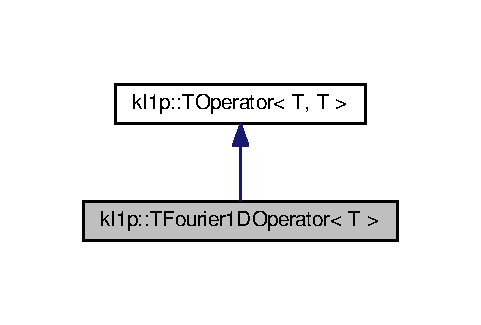
\includegraphics[width=231pt]{classkl1p_1_1TFourier1DOperator__inherit__graph}
\end{center}
\end{figure}


Collaboration diagram for kl1p\+:\+:T\+Fourier1\+D\+Operator$<$ T $>$\+:
\nopagebreak
\begin{figure}[H]
\begin{center}
\leavevmode
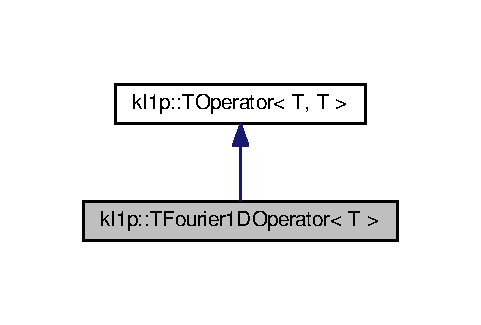
\includegraphics[width=231pt]{classkl1p_1_1TFourier1DOperator__coll__graph}
\end{center}
\end{figure}
\subsection*{Public Member Functions}
\begin{DoxyCompactItemize}
\item 
{\bfseries T\+Fourier1\+D\+Operator} (klab\+::\+U\+Int32 n)\hypertarget{classkl1p_1_1TFourier1DOperator_a1c9fea760a7954bd3b06c40b6b74468d}{}\label{classkl1p_1_1TFourier1DOperator_a1c9fea760a7954bd3b06c40b6b74468d}

\item 
{\bfseries T\+Fourier1\+D\+Operator} (klab\+::\+U\+Int32 n, bool shift)\hypertarget{classkl1p_1_1TFourier1DOperator_abc86ecbb37c95d7e99ac905b7175dd8a}{}\label{classkl1p_1_1TFourier1DOperator_abc86ecbb37c95d7e99ac905b7175dd8a}

\item 
{\bfseries T\+Fourier1\+D\+Operator} (const \hyperlink{classkl1p_1_1TFourier1DOperator}{T\+Fourier1\+D\+Operator}$<$ T $>$ \&op)\hypertarget{classkl1p_1_1TFourier1DOperator_a4528ebf2d0aaed922d32a861880fd8e0}{}\label{classkl1p_1_1TFourier1DOperator_a4528ebf2d0aaed922d32a861880fd8e0}

\item 
bool {\bfseries is\+Shift} () const \hypertarget{classkl1p_1_1TFourier1DOperator_ae32414af3c074092e3478817baace71a}{}\label{classkl1p_1_1TFourier1DOperator_ae32414af3c074092e3478817baace71a}

\item 
virtual void {\bfseries apply} (const arma\+::\+Col$<$ T $>$ \&in, arma\+::\+Col$<$ T $>$ \&out)\hypertarget{classkl1p_1_1TFourier1DOperator_ae10c86766d42453672c558d92c08d51a}{}\label{classkl1p_1_1TFourier1DOperator_ae10c86766d42453672c558d92c08d51a}

\item 
virtual void {\bfseries apply\+Adjoint} (const arma\+::\+Col$<$ T $>$ \&in, arma\+::\+Col$<$ T $>$ \&out)\hypertarget{classkl1p_1_1TFourier1DOperator_a852c3195f47ce84f09d7fbf333153eaf}{}\label{classkl1p_1_1TFourier1DOperator_a852c3195f47ce84f09d7fbf333153eaf}

\end{DoxyCompactItemize}
\subsection*{Additional Inherited Members}


The documentation for this class was generated from the following file\+:\begin{DoxyCompactItemize}
\item 
include/Fourier1\+D\+Operator.\+h\end{DoxyCompactItemize}

\hypertarget{classkl1p_1_1TFourier1DOperatorSpecialisation}{}\section{kl1p\+:\+:T\+Fourier1\+D\+Operator\+Specialisation$<$ T $>$ Class Template Reference}
\label{classkl1p_1_1TFourier1DOperatorSpecialisation}\index{kl1p\+::\+T\+Fourier1\+D\+Operator\+Specialisation$<$ T $>$@{kl1p\+::\+T\+Fourier1\+D\+Operator\+Specialisation$<$ T $>$}}
\subsection*{Static Public Member Functions}
\begin{DoxyCompactItemize}
\item 
static void {\bfseries Apply\+Adjoint} (const arma\+::\+Col$<$ T $>$ \&in, arma\+::\+Col$<$ T $>$ \&out, klab\+::\+T\+F\+F\+T1D$<$ T $>$ \&fft)\hypertarget{classkl1p_1_1TFourier1DOperatorSpecialisation_a1c674c79f72d7833ca5067bdd9888db5}{}\label{classkl1p_1_1TFourier1DOperatorSpecialisation_a1c674c79f72d7833ca5067bdd9888db5}

\end{DoxyCompactItemize}


The documentation for this class was generated from the following file\+:\begin{DoxyCompactItemize}
\item 
include/Fourier1\+D\+Operator.\+h\end{DoxyCompactItemize}

\hypertarget{classkl1p_1_1TFourier1DOperatorSpecialisation_3_01std_1_1complex_3_01T_01_4_01_4}{}\section{kl1p\+:\+:T\+Fourier1\+D\+Operator\+Specialisation$<$ std\+:\+:complex$<$ T $>$ $>$ Class Template Reference}
\label{classkl1p_1_1TFourier1DOperatorSpecialisation_3_01std_1_1complex_3_01T_01_4_01_4}\index{kl1p\+::\+T\+Fourier1\+D\+Operator\+Specialisation$<$ std\+::complex$<$ T $>$ $>$@{kl1p\+::\+T\+Fourier1\+D\+Operator\+Specialisation$<$ std\+::complex$<$ T $>$ $>$}}
\subsection*{Static Public Member Functions}
\begin{DoxyCompactItemize}
\item 
static void {\bfseries Apply\+Adjoint} (const arma\+::\+Col$<$ std\+::complex$<$ T $>$ $>$ \&in, arma\+::\+Col$<$ std\+::complex$<$ T $>$ $>$ \&out, klab\+::\+T\+F\+F\+T1D$<$ std\+::complex$<$ T $>$ $>$ \&fft)\hypertarget{classkl1p_1_1TFourier1DOperatorSpecialisation_3_01std_1_1complex_3_01T_01_4_01_4_a75bfac6795d2d94b7842cf5b417f0f48}{}\label{classkl1p_1_1TFourier1DOperatorSpecialisation_3_01std_1_1complex_3_01T_01_4_01_4_a75bfac6795d2d94b7842cf5b417f0f48}

\end{DoxyCompactItemize}


The documentation for this class was generated from the following file\+:\begin{DoxyCompactItemize}
\item 
include/Fourier1\+D\+Operator.\+h\end{DoxyCompactItemize}

\hypertarget{classkl1p_1_1TFourier2DOperator}{}\section{kl1p\+:\+:T\+Fourier2\+D\+Operator$<$ T $>$ Class Template Reference}
\label{classkl1p_1_1TFourier2DOperator}\index{kl1p\+::\+T\+Fourier2\+D\+Operator$<$ T $>$@{kl1p\+::\+T\+Fourier2\+D\+Operator$<$ T $>$}}


Inheritance diagram for kl1p\+:\+:T\+Fourier2\+D\+Operator$<$ T $>$\+:
\nopagebreak
\begin{figure}[H]
\begin{center}
\leavevmode
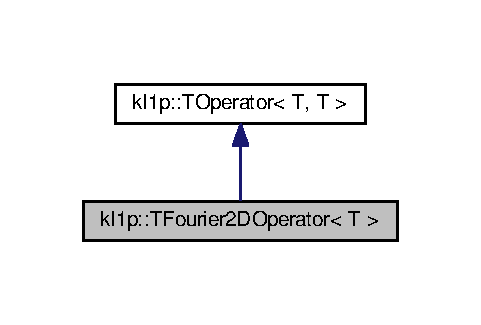
\includegraphics[width=231pt]{classkl1p_1_1TFourier2DOperator__inherit__graph}
\end{center}
\end{figure}


Collaboration diagram for kl1p\+:\+:T\+Fourier2\+D\+Operator$<$ T $>$\+:
\nopagebreak
\begin{figure}[H]
\begin{center}
\leavevmode
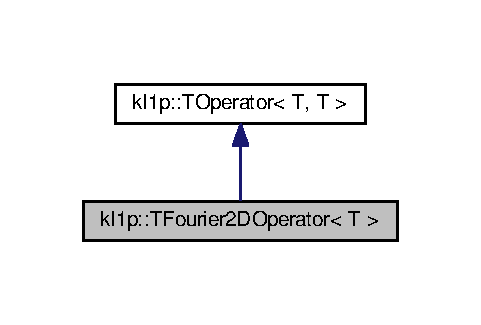
\includegraphics[width=231pt]{classkl1p_1_1TFourier2DOperator__coll__graph}
\end{center}
\end{figure}
\subsection*{Public Member Functions}
\begin{DoxyCompactItemize}
\item 
{\bfseries T\+Fourier2\+D\+Operator} (klab\+::\+U\+Int32 height, klab\+::\+U\+Int32 width, bool shift=false)\hypertarget{classkl1p_1_1TFourier2DOperator_a6a73d4b903ddd31eb90230e0dc97e413}{}\label{classkl1p_1_1TFourier2DOperator_a6a73d4b903ddd31eb90230e0dc97e413}

\item 
{\bfseries T\+Fourier2\+D\+Operator} (const \hyperlink{classkl1p_1_1TFourier2DOperator}{T\+Fourier2\+D\+Operator}$<$ T $>$ \&op)\hypertarget{classkl1p_1_1TFourier2DOperator_a9b7a2f6ab9bacef945efcfe01a508d37}{}\label{classkl1p_1_1TFourier2DOperator_a9b7a2f6ab9bacef945efcfe01a508d37}

\item 
klab\+::\+U\+Int32 {\bfseries width} () const \hypertarget{classkl1p_1_1TFourier2DOperator_a4cd8f04a032c960710bc7805df430b48}{}\label{classkl1p_1_1TFourier2DOperator_a4cd8f04a032c960710bc7805df430b48}

\item 
klab\+::\+U\+Int32 {\bfseries height} () const \hypertarget{classkl1p_1_1TFourier2DOperator_a45edca0dbdd0cac051b5e27cf511c91e}{}\label{classkl1p_1_1TFourier2DOperator_a45edca0dbdd0cac051b5e27cf511c91e}

\item 
bool {\bfseries is\+Shift} () const \hypertarget{classkl1p_1_1TFourier2DOperator_a2f38d8c1107c3af9d3b40d6cb3de9723}{}\label{classkl1p_1_1TFourier2DOperator_a2f38d8c1107c3af9d3b40d6cb3de9723}

\item 
virtual void {\bfseries apply} (const arma\+::\+Col$<$ T $>$ \&in, arma\+::\+Col$<$ T $>$ \&out)\hypertarget{classkl1p_1_1TFourier2DOperator_abb5a6de2d0d1b304edc7b624e60faf2b}{}\label{classkl1p_1_1TFourier2DOperator_abb5a6de2d0d1b304edc7b624e60faf2b}

\item 
virtual void {\bfseries apply\+Adjoint} (const arma\+::\+Col$<$ T $>$ \&in, arma\+::\+Col$<$ T $>$ \&out)\hypertarget{classkl1p_1_1TFourier2DOperator_a0e0838aaaf40a283752f7dae9f36f39c}{}\label{classkl1p_1_1TFourier2DOperator_a0e0838aaaf40a283752f7dae9f36f39c}

\end{DoxyCompactItemize}
\subsection*{Additional Inherited Members}


The documentation for this class was generated from the following file\+:\begin{DoxyCompactItemize}
\item 
include/Fourier2\+D\+Operator.\+h\end{DoxyCompactItemize}

\hypertarget{classkl1p_1_1TFourier2DOperatorSpecialisation}{}\section{kl1p\+:\+:T\+Fourier2\+D\+Operator\+Specialisation$<$ T $>$ Class Template Reference}
\label{classkl1p_1_1TFourier2DOperatorSpecialisation}\index{kl1p\+::\+T\+Fourier2\+D\+Operator\+Specialisation$<$ T $>$@{kl1p\+::\+T\+Fourier2\+D\+Operator\+Specialisation$<$ T $>$}}
\subsection*{Static Public Member Functions}
\begin{DoxyCompactItemize}
\item 
static void {\bfseries Apply\+Adjoint} (const arma\+::\+Col$<$ T $>$ \&in, arma\+::\+Col$<$ T $>$ \&out, klab\+::\+U\+Int32 height, klab\+::\+U\+Int32 width, klab\+::\+T\+F\+F\+T2D$<$ T $>$ \&fft)\hypertarget{classkl1p_1_1TFourier2DOperatorSpecialisation_aa9b5fe7e102c0108addca9d306e7953f}{}\label{classkl1p_1_1TFourier2DOperatorSpecialisation_aa9b5fe7e102c0108addca9d306e7953f}

\end{DoxyCompactItemize}


The documentation for this class was generated from the following file\+:\begin{DoxyCompactItemize}
\item 
include/Fourier2\+D\+Operator.\+h\end{DoxyCompactItemize}

\hypertarget{classkl1p_1_1TFourier2DOperatorSpecialisation_3_01std_1_1complex_3_01T_01_4_01_4}{}\section{kl1p\+:\+:T\+Fourier2\+D\+Operator\+Specialisation$<$ std\+:\+:complex$<$ T $>$ $>$ Class Template Reference}
\label{classkl1p_1_1TFourier2DOperatorSpecialisation_3_01std_1_1complex_3_01T_01_4_01_4}\index{kl1p\+::\+T\+Fourier2\+D\+Operator\+Specialisation$<$ std\+::complex$<$ T $>$ $>$@{kl1p\+::\+T\+Fourier2\+D\+Operator\+Specialisation$<$ std\+::complex$<$ T $>$ $>$}}
\subsection*{Static Public Member Functions}
\begin{DoxyCompactItemize}
\item 
static void {\bfseries Apply\+Adjoint} (const arma\+::\+Col$<$ std\+::complex$<$ T $>$ $>$ \&in, arma\+::\+Col$<$ std\+::complex$<$ T $>$ $>$ \&out, klab\+::\+U\+Int32 height, klab\+::\+U\+Int32 width, klab\+::\+T\+F\+F\+T2D$<$ std\+::complex$<$ T $>$ $>$ \&fft)\hypertarget{classkl1p_1_1TFourier2DOperatorSpecialisation_3_01std_1_1complex_3_01T_01_4_01_4_a8009fbf9e8804e49af45e3a4846e17b2}{}\label{classkl1p_1_1TFourier2DOperatorSpecialisation_3_01std_1_1complex_3_01T_01_4_01_4_a8009fbf9e8804e49af45e3a4846e17b2}

\end{DoxyCompactItemize}


The documentation for this class was generated from the following file\+:\begin{DoxyCompactItemize}
\item 
include/Fourier2\+D\+Operator.\+h\end{DoxyCompactItemize}

\hypertarget{classkl1p_1_1TGaussian1DDiagonalOperator}{}\section{kl1p\+:\+:T\+Gaussian1\+D\+Diagonal\+Operator$<$ T $>$ Class Template Reference}
\label{classkl1p_1_1TGaussian1DDiagonalOperator}\index{kl1p\+::\+T\+Gaussian1\+D\+Diagonal\+Operator$<$ T $>$@{kl1p\+::\+T\+Gaussian1\+D\+Diagonal\+Operator$<$ T $>$}}


Inheritance diagram for kl1p\+:\+:T\+Gaussian1\+D\+Diagonal\+Operator$<$ T $>$\+:
\nopagebreak
\begin{figure}[H]
\begin{center}
\leavevmode
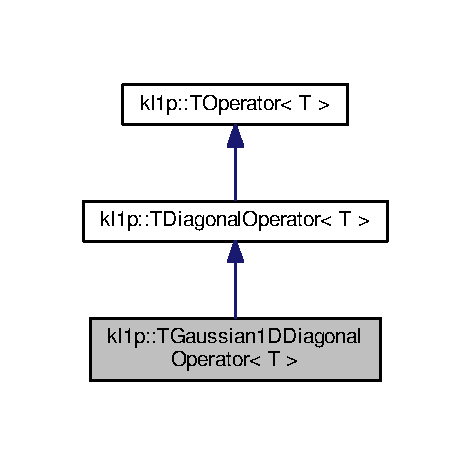
\includegraphics[width=226pt]{classkl1p_1_1TGaussian1DDiagonalOperator__inherit__graph}
\end{center}
\end{figure}


Collaboration diagram for kl1p\+:\+:T\+Gaussian1\+D\+Diagonal\+Operator$<$ T $>$\+:
\nopagebreak
\begin{figure}[H]
\begin{center}
\leavevmode
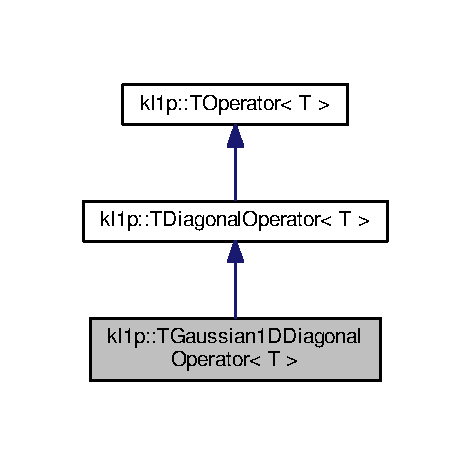
\includegraphics[width=226pt]{classkl1p_1_1TGaussian1DDiagonalOperator__coll__graph}
\end{center}
\end{figure}
\subsection*{Public Member Functions}
\begin{DoxyCompactItemize}
\item 
{\bfseries T\+Gaussian1\+D\+Diagonal\+Operator} (klab\+::\+U\+Int32 n)\hypertarget{classkl1p_1_1TGaussian1DDiagonalOperator_a9662b11615037f761673a5b996a8d7f3}{}\label{classkl1p_1_1TGaussian1DDiagonalOperator_a9662b11615037f761673a5b996a8d7f3}

\item 
{\bfseries T\+Gaussian1\+D\+Diagonal\+Operator} (klab\+::\+U\+Int32 n, const T \&sigma)\hypertarget{classkl1p_1_1TGaussian1DDiagonalOperator_ac7320e45fa7f069475059800e7582387}{}\label{classkl1p_1_1TGaussian1DDiagonalOperator_ac7320e45fa7f069475059800e7582387}

\item 
{\bfseries T\+Gaussian1\+D\+Diagonal\+Operator} (klab\+::\+U\+Int32 n, const T \&sigma, klab\+::\+Int32 c)\hypertarget{classkl1p_1_1TGaussian1DDiagonalOperator_aa8db33138463100399a767cfce4cbe18}{}\label{classkl1p_1_1TGaussian1DDiagonalOperator_aa8db33138463100399a767cfce4cbe18}

\item 
{\bfseries T\+Gaussian1\+D\+Diagonal\+Operator} (const \hyperlink{classkl1p_1_1TGaussian1DDiagonalOperator}{T\+Gaussian1\+D\+Diagonal\+Operator}$<$ T $>$ \&op)\hypertarget{classkl1p_1_1TGaussian1DDiagonalOperator_a15d57ae2d1f326e3b5bde32fb5ee3377}{}\label{classkl1p_1_1TGaussian1DDiagonalOperator_a15d57ae2d1f326e3b5bde32fb5ee3377}

\item 
const T \& {\bfseries sigma} () const \hypertarget{classkl1p_1_1TGaussian1DDiagonalOperator_a0c773e8664dcb056abd4a5187458dd8c}{}\label{classkl1p_1_1TGaussian1DDiagonalOperator_a0c773e8664dcb056abd4a5187458dd8c}

\item 
klab\+::\+Int32 {\bfseries c} () const \hypertarget{classkl1p_1_1TGaussian1DDiagonalOperator_ad0532976037c07ae19f8e1821734b4f4}{}\label{classkl1p_1_1TGaussian1DDiagonalOperator_ad0532976037c07ae19f8e1821734b4f4}

\end{DoxyCompactItemize}
\subsection*{Additional Inherited Members}


The documentation for this class was generated from the following file\+:\begin{DoxyCompactItemize}
\item 
include/Gaussian1\+D\+Diagonal\+Operator.\+h\end{DoxyCompactItemize}

\hypertarget{classkl1p_1_1TGaussian2DDiagonalOperator}{}\section{kl1p\+:\+:T\+Gaussian2\+D\+Diagonal\+Operator$<$ T $>$ Class Template Reference}
\label{classkl1p_1_1TGaussian2DDiagonalOperator}\index{kl1p\+::\+T\+Gaussian2\+D\+Diagonal\+Operator$<$ T $>$@{kl1p\+::\+T\+Gaussian2\+D\+Diagonal\+Operator$<$ T $>$}}


Inheritance diagram for kl1p\+:\+:T\+Gaussian2\+D\+Diagonal\+Operator$<$ T $>$\+:
\nopagebreak
\begin{figure}[H]
\begin{center}
\leavevmode
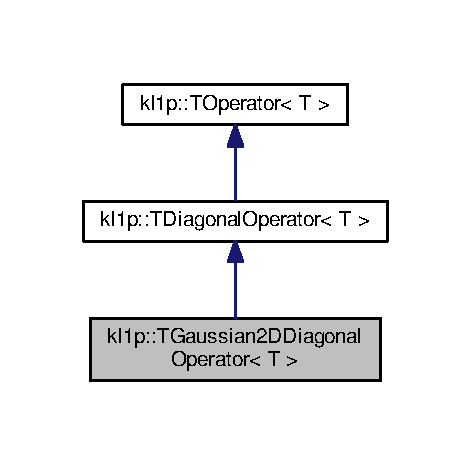
\includegraphics[width=226pt]{classkl1p_1_1TGaussian2DDiagonalOperator__inherit__graph}
\end{center}
\end{figure}


Collaboration diagram for kl1p\+:\+:T\+Gaussian2\+D\+Diagonal\+Operator$<$ T $>$\+:
\nopagebreak
\begin{figure}[H]
\begin{center}
\leavevmode
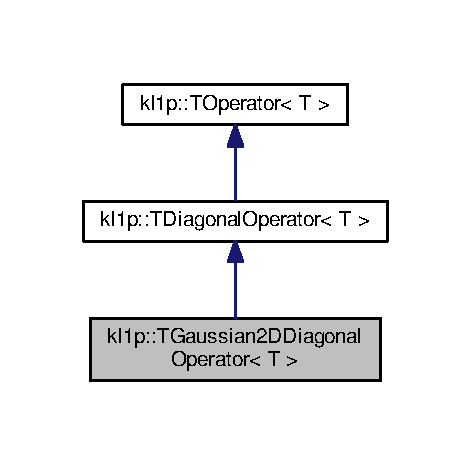
\includegraphics[width=226pt]{classkl1p_1_1TGaussian2DDiagonalOperator__coll__graph}
\end{center}
\end{figure}
\subsection*{Public Member Functions}
\begin{DoxyCompactItemize}
\item 
{\bfseries T\+Gaussian2\+D\+Diagonal\+Operator} (klab\+::\+U\+Int32 height, klab\+::\+U\+Int32 width)\hypertarget{classkl1p_1_1TGaussian2DDiagonalOperator_a47969ffab3aab03fb66a28dda0226526}{}\label{classkl1p_1_1TGaussian2DDiagonalOperator_a47969ffab3aab03fb66a28dda0226526}

\item 
{\bfseries T\+Gaussian2\+D\+Diagonal\+Operator} (klab\+::\+U\+Int32 height, klab\+::\+U\+Int32 width, const T \&sigma)\hypertarget{classkl1p_1_1TGaussian2DDiagonalOperator_a34982072d8ebfa327bb76d8fe1588fe7}{}\label{classkl1p_1_1TGaussian2DDiagonalOperator_a34982072d8ebfa327bb76d8fe1588fe7}

\item 
{\bfseries T\+Gaussian2\+D\+Diagonal\+Operator} (klab\+::\+U\+Int32 height, klab\+::\+U\+Int32 width, const T \&sigma, klab\+::\+Int32 ic, klab\+::\+Int32 jc)\hypertarget{classkl1p_1_1TGaussian2DDiagonalOperator_ab332c84617d8df607d5cfa6ff435801e}{}\label{classkl1p_1_1TGaussian2DDiagonalOperator_ab332c84617d8df607d5cfa6ff435801e}

\item 
{\bfseries T\+Gaussian2\+D\+Diagonal\+Operator} (const \hyperlink{classkl1p_1_1TGaussian2DDiagonalOperator}{T\+Gaussian2\+D\+Diagonal\+Operator}$<$ T $>$ \&op)\hypertarget{classkl1p_1_1TGaussian2DDiagonalOperator_aef45ac6c473e95655f3aedf58e0fcc51}{}\label{classkl1p_1_1TGaussian2DDiagonalOperator_aef45ac6c473e95655f3aedf58e0fcc51}

\item 
klab\+::\+U\+Int32 {\bfseries width} () const \hypertarget{classkl1p_1_1TGaussian2DDiagonalOperator_a858ffa3571b73fd6b89331da02a44ce7}{}\label{classkl1p_1_1TGaussian2DDiagonalOperator_a858ffa3571b73fd6b89331da02a44ce7}

\item 
klab\+::\+U\+Int32 {\bfseries height} () const \hypertarget{classkl1p_1_1TGaussian2DDiagonalOperator_ae03846d27549fc22264b7eee2092ab35}{}\label{classkl1p_1_1TGaussian2DDiagonalOperator_ae03846d27549fc22264b7eee2092ab35}

\item 
const T \& {\bfseries sigma} () const \hypertarget{classkl1p_1_1TGaussian2DDiagonalOperator_a206603bbc13aa9e794367b2bf2d90f19}{}\label{classkl1p_1_1TGaussian2DDiagonalOperator_a206603bbc13aa9e794367b2bf2d90f19}

\item 
klab\+::\+Int32 {\bfseries ic} () const \hypertarget{classkl1p_1_1TGaussian2DDiagonalOperator_a7579932430acc2f14bf0edf184d43415}{}\label{classkl1p_1_1TGaussian2DDiagonalOperator_a7579932430acc2f14bf0edf184d43415}

\item 
klab\+::\+Int32 {\bfseries jc} () const \hypertarget{classkl1p_1_1TGaussian2DDiagonalOperator_af4f85759c421d40fec1a8ae1bb6a30b6}{}\label{classkl1p_1_1TGaussian2DDiagonalOperator_af4f85759c421d40fec1a8ae1bb6a30b6}

\end{DoxyCompactItemize}
\subsection*{Additional Inherited Members}


The documentation for this class was generated from the following file\+:\begin{DoxyCompactItemize}
\item 
include/Gaussian2\+D\+Diagonal\+Operator.\+h\end{DoxyCompactItemize}

\hypertarget{classkl1p_1_1TGaussianBlur1DOperator}{}\section{kl1p\+:\+:T\+Gaussian\+Blur1\+D\+Operator$<$ T $>$ Class Template Reference}
\label{classkl1p_1_1TGaussianBlur1DOperator}\index{kl1p\+::\+T\+Gaussian\+Blur1\+D\+Operator$<$ T $>$@{kl1p\+::\+T\+Gaussian\+Blur1\+D\+Operator$<$ T $>$}}


Inheritance diagram for kl1p\+:\+:T\+Gaussian\+Blur1\+D\+Operator$<$ T $>$\+:
\nopagebreak
\begin{figure}[H]
\begin{center}
\leavevmode
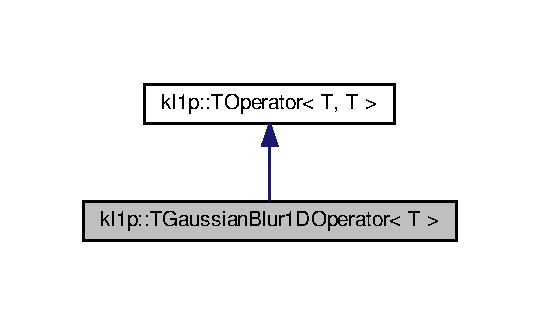
\includegraphics[width=259pt]{classkl1p_1_1TGaussianBlur1DOperator__inherit__graph}
\end{center}
\end{figure}


Collaboration diagram for kl1p\+:\+:T\+Gaussian\+Blur1\+D\+Operator$<$ T $>$\+:
\nopagebreak
\begin{figure}[H]
\begin{center}
\leavevmode
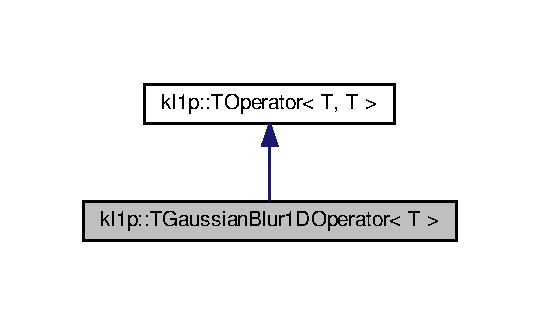
\includegraphics[width=259pt]{classkl1p_1_1TGaussianBlur1DOperator__coll__graph}
\end{center}
\end{figure}
\subsection*{Public Member Functions}
\begin{DoxyCompactItemize}
\item 
{\bfseries T\+Gaussian\+Blur1\+D\+Operator} (klab\+::\+U\+Int32 n)\hypertarget{classkl1p_1_1TGaussianBlur1DOperator_adfce593c12eed171d36fc4c644b46581}{}\label{classkl1p_1_1TGaussianBlur1DOperator_adfce593c12eed171d36fc4c644b46581}

\item 
{\bfseries T\+Gaussian\+Blur1\+D\+Operator} (klab\+::\+U\+Int32 n, const T \&sigma)\hypertarget{classkl1p_1_1TGaussianBlur1DOperator_a6bbbb52566ad498961cea10eb41cd3c6}{}\label{classkl1p_1_1TGaussianBlur1DOperator_a6bbbb52566ad498961cea10eb41cd3c6}

\item 
{\bfseries T\+Gaussian\+Blur1\+D\+Operator} (klab\+::\+U\+Int32 n, const T \&sigma, klab\+::\+Int32 c)\hypertarget{classkl1p_1_1TGaussianBlur1DOperator_a46967bf1040233065f9632491112258f}{}\label{classkl1p_1_1TGaussianBlur1DOperator_a46967bf1040233065f9632491112258f}

\item 
{\bfseries T\+Gaussian\+Blur1\+D\+Operator} (const \hyperlink{classkl1p_1_1TGaussianBlur1DOperator}{T\+Gaussian\+Blur1\+D\+Operator}$<$ T $>$ \&op)\hypertarget{classkl1p_1_1TGaussianBlur1DOperator_a15736b401979249a7db00f56106bab68}{}\label{classkl1p_1_1TGaussianBlur1DOperator_a15736b401979249a7db00f56106bab68}

\item 
T {\bfseries sigma} () const \hypertarget{classkl1p_1_1TGaussianBlur1DOperator_aff4f98560b1abb8ea038b0e7ce862be5}{}\label{classkl1p_1_1TGaussianBlur1DOperator_aff4f98560b1abb8ea038b0e7ce862be5}

\item 
klab\+::\+Int32 {\bfseries c} () const \hypertarget{classkl1p_1_1TGaussianBlur1DOperator_aee24e5571d642bfc3f418b85f84638f4}{}\label{classkl1p_1_1TGaussianBlur1DOperator_aee24e5571d642bfc3f418b85f84638f4}

\item 
virtual void {\bfseries apply} (const arma\+::\+Col$<$ T $>$ \&in, arma\+::\+Col$<$ T $>$ \&out)\hypertarget{classkl1p_1_1TGaussianBlur1DOperator_afa148df1de62ae6c874b2545faf7e781}{}\label{classkl1p_1_1TGaussianBlur1DOperator_afa148df1de62ae6c874b2545faf7e781}

\item 
virtual void {\bfseries apply\+Adjoint} (const arma\+::\+Col$<$ T $>$ \&in, arma\+::\+Col$<$ T $>$ \&out)\hypertarget{classkl1p_1_1TGaussianBlur1DOperator_ae81016302a1de4d81a629ff5f9f2c0e1}{}\label{classkl1p_1_1TGaussianBlur1DOperator_ae81016302a1de4d81a629ff5f9f2c0e1}

\end{DoxyCompactItemize}
\subsection*{Additional Inherited Members}


The documentation for this class was generated from the following file\+:\begin{DoxyCompactItemize}
\item 
include/Gaussian\+Blur1\+D\+Operator.\+h\end{DoxyCompactItemize}

\hypertarget{classkl1p_1_1TGaussianBlur1DOperator_3_01std_1_1complex_3_01T_01_4_01_4}{}\section{kl1p\+:\+:T\+Gaussian\+Blur1\+D\+Operator$<$ std\+:\+:complex$<$ T $>$ $>$ Class Template Reference}
\label{classkl1p_1_1TGaussianBlur1DOperator_3_01std_1_1complex_3_01T_01_4_01_4}\index{kl1p\+::\+T\+Gaussian\+Blur1\+D\+Operator$<$ std\+::complex$<$ T $>$ $>$@{kl1p\+::\+T\+Gaussian\+Blur1\+D\+Operator$<$ std\+::complex$<$ T $>$ $>$}}


Inheritance diagram for kl1p\+:\+:T\+Gaussian\+Blur1\+D\+Operator$<$ std\+:\+:complex$<$ T $>$ $>$\+:
\nopagebreak
\begin{figure}[H]
\begin{center}
\leavevmode
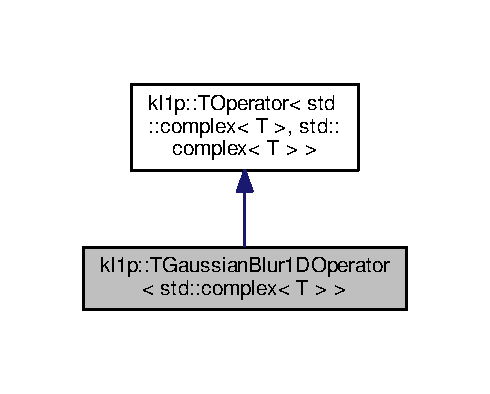
\includegraphics[width=235pt]{classkl1p_1_1TGaussianBlur1DOperator_3_01std_1_1complex_3_01T_01_4_01_4__inherit__graph}
\end{center}
\end{figure}


Collaboration diagram for kl1p\+:\+:T\+Gaussian\+Blur1\+D\+Operator$<$ std\+:\+:complex$<$ T $>$ $>$\+:
\nopagebreak
\begin{figure}[H]
\begin{center}
\leavevmode
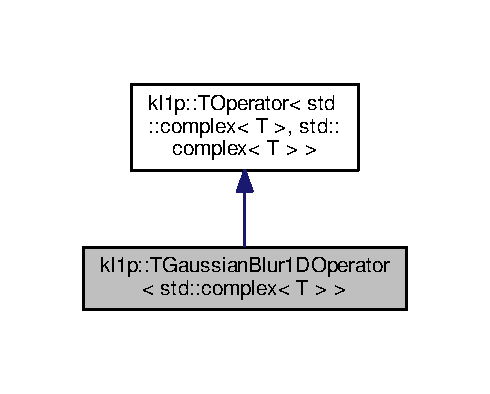
\includegraphics[width=235pt]{classkl1p_1_1TGaussianBlur1DOperator_3_01std_1_1complex_3_01T_01_4_01_4__coll__graph}
\end{center}
\end{figure}
\subsection*{Public Member Functions}
\begin{DoxyCompactItemize}
\item 
{\bfseries T\+Gaussian\+Blur1\+D\+Operator} (klab\+::\+U\+Int32 n)\hypertarget{classkl1p_1_1TGaussianBlur1DOperator_3_01std_1_1complex_3_01T_01_4_01_4_a6ef3d0d3ff105466a7a38582810bec13}{}\label{classkl1p_1_1TGaussianBlur1DOperator_3_01std_1_1complex_3_01T_01_4_01_4_a6ef3d0d3ff105466a7a38582810bec13}

\item 
{\bfseries T\+Gaussian\+Blur1\+D\+Operator} (klab\+::\+U\+Int32 n, const std\+::complex$<$ T $>$ \&sigma)\hypertarget{classkl1p_1_1TGaussianBlur1DOperator_3_01std_1_1complex_3_01T_01_4_01_4_a76879772e51d6575c677f050ea32e076}{}\label{classkl1p_1_1TGaussianBlur1DOperator_3_01std_1_1complex_3_01T_01_4_01_4_a76879772e51d6575c677f050ea32e076}

\item 
{\bfseries T\+Gaussian\+Blur1\+D\+Operator} (klab\+::\+U\+Int32 n, const std\+::complex$<$ T $>$ \&sigma, klab\+::\+Int32 c)\hypertarget{classkl1p_1_1TGaussianBlur1DOperator_3_01std_1_1complex_3_01T_01_4_01_4_ac84daca7243fd87bf6a00211b19fbb38}{}\label{classkl1p_1_1TGaussianBlur1DOperator_3_01std_1_1complex_3_01T_01_4_01_4_ac84daca7243fd87bf6a00211b19fbb38}

\item 
{\bfseries T\+Gaussian\+Blur1\+D\+Operator} (const \hyperlink{classkl1p_1_1TGaussianBlur1DOperator}{T\+Gaussian\+Blur1\+D\+Operator}$<$ std\+::complex$<$ T $>$ $>$ \&op)\hypertarget{classkl1p_1_1TGaussianBlur1DOperator_3_01std_1_1complex_3_01T_01_4_01_4_ad5d3d346f0b1c01daadf238dfa5ba5c5}{}\label{classkl1p_1_1TGaussianBlur1DOperator_3_01std_1_1complex_3_01T_01_4_01_4_ad5d3d346f0b1c01daadf238dfa5ba5c5}

\item 
klab\+::\+U\+Int32 {\bfseries size} () const \hypertarget{classkl1p_1_1TGaussianBlur1DOperator_3_01std_1_1complex_3_01T_01_4_01_4_a6ad95a5d2c231039c2681249ff7d3806}{}\label{classkl1p_1_1TGaussianBlur1DOperator_3_01std_1_1complex_3_01T_01_4_01_4_a6ad95a5d2c231039c2681249ff7d3806}

\item 
std\+::complex$<$ T $>$ {\bfseries sigma} () const \hypertarget{classkl1p_1_1TGaussianBlur1DOperator_3_01std_1_1complex_3_01T_01_4_01_4_a14659e1611e0ea131fc595790e8a48b3}{}\label{classkl1p_1_1TGaussianBlur1DOperator_3_01std_1_1complex_3_01T_01_4_01_4_a14659e1611e0ea131fc595790e8a48b3}

\item 
klab\+::\+Int32 {\bfseries c} () const \hypertarget{classkl1p_1_1TGaussianBlur1DOperator_3_01std_1_1complex_3_01T_01_4_01_4_a0fd1f8d7fe4f0bf58f111c59b594ef83}{}\label{classkl1p_1_1TGaussianBlur1DOperator_3_01std_1_1complex_3_01T_01_4_01_4_a0fd1f8d7fe4f0bf58f111c59b594ef83}

\item 
virtual void {\bfseries apply} (const arma\+::\+Col$<$ std\+::complex$<$ T $>$ $>$ \&in, arma\+::\+Col$<$ std\+::complex$<$ T $>$ $>$ \&out)\hypertarget{classkl1p_1_1TGaussianBlur1DOperator_3_01std_1_1complex_3_01T_01_4_01_4_a00ec47be955735371b27301529dd7f29}{}\label{classkl1p_1_1TGaussianBlur1DOperator_3_01std_1_1complex_3_01T_01_4_01_4_a00ec47be955735371b27301529dd7f29}

\item 
virtual void {\bfseries apply\+Adjoint} (const arma\+::\+Col$<$ std\+::complex$<$ T $>$ $>$ \&in, arma\+::\+Col$<$ std\+::complex$<$ T $>$ $>$ \&out)\hypertarget{classkl1p_1_1TGaussianBlur1DOperator_3_01std_1_1complex_3_01T_01_4_01_4_a1e2868cf66b78473da6482ae1202d1fb}{}\label{classkl1p_1_1TGaussianBlur1DOperator_3_01std_1_1complex_3_01T_01_4_01_4_a1e2868cf66b78473da6482ae1202d1fb}

\end{DoxyCompactItemize}
\subsection*{Additional Inherited Members}


The documentation for this class was generated from the following file\+:\begin{DoxyCompactItemize}
\item 
include/Gaussian\+Blur1\+D\+Operator.\+h\end{DoxyCompactItemize}

\hypertarget{classkl1p_1_1TGaussianBlur2DOperator}{}\section{kl1p\+:\+:T\+Gaussian\+Blur2\+D\+Operator$<$ T $>$ Class Template Reference}
\label{classkl1p_1_1TGaussianBlur2DOperator}\index{kl1p\+::\+T\+Gaussian\+Blur2\+D\+Operator$<$ T $>$@{kl1p\+::\+T\+Gaussian\+Blur2\+D\+Operator$<$ T $>$}}


Inheritance diagram for kl1p\+:\+:T\+Gaussian\+Blur2\+D\+Operator$<$ T $>$\+:
\nopagebreak
\begin{figure}[H]
\begin{center}
\leavevmode
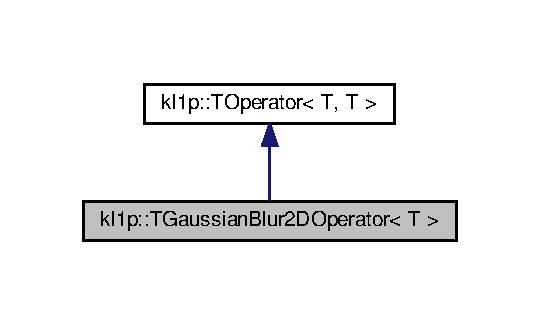
\includegraphics[width=259pt]{classkl1p_1_1TGaussianBlur2DOperator__inherit__graph}
\end{center}
\end{figure}


Collaboration diagram for kl1p\+:\+:T\+Gaussian\+Blur2\+D\+Operator$<$ T $>$\+:
\nopagebreak
\begin{figure}[H]
\begin{center}
\leavevmode
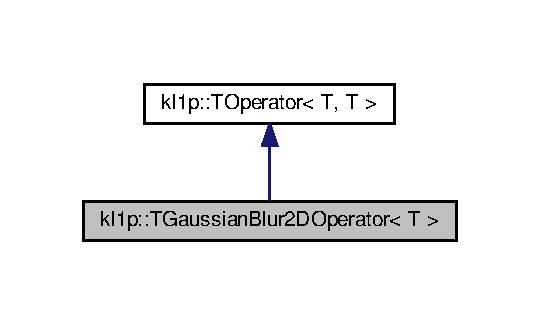
\includegraphics[width=259pt]{classkl1p_1_1TGaussianBlur2DOperator__coll__graph}
\end{center}
\end{figure}
\subsection*{Public Member Functions}
\begin{DoxyCompactItemize}
\item 
{\bfseries T\+Gaussian\+Blur2\+D\+Operator} (klab\+::\+U\+Int32 height, klab\+::\+U\+Int32 width)\hypertarget{classkl1p_1_1TGaussianBlur2DOperator_a865a2ce1fb6cf509a69b956c8f939f95}{}\label{classkl1p_1_1TGaussianBlur2DOperator_a865a2ce1fb6cf509a69b956c8f939f95}

\item 
{\bfseries T\+Gaussian\+Blur2\+D\+Operator} (klab\+::\+U\+Int32 height, klab\+::\+U\+Int32 width, const T \&sigma)\hypertarget{classkl1p_1_1TGaussianBlur2DOperator_ae76cd1b72456270dab3c0c556c4accdf}{}\label{classkl1p_1_1TGaussianBlur2DOperator_ae76cd1b72456270dab3c0c556c4accdf}

\item 
{\bfseries T\+Gaussian\+Blur2\+D\+Operator} (klab\+::\+U\+Int32 height, klab\+::\+U\+Int32 width, const T \&sigma, klab\+::\+Int32 ic, klab\+::\+Int32 jc)\hypertarget{classkl1p_1_1TGaussianBlur2DOperator_a63e8ccb771b703b31a788ce2c80867f6}{}\label{classkl1p_1_1TGaussianBlur2DOperator_a63e8ccb771b703b31a788ce2c80867f6}

\item 
{\bfseries T\+Gaussian\+Blur2\+D\+Operator} (const \hyperlink{classkl1p_1_1TGaussianBlur2DOperator}{T\+Gaussian\+Blur2\+D\+Operator}$<$ T $>$ \&op)\hypertarget{classkl1p_1_1TGaussianBlur2DOperator_a1402713b9c3e03697ae535faa7e6ee10}{}\label{classkl1p_1_1TGaussianBlur2DOperator_a1402713b9c3e03697ae535faa7e6ee10}

\item 
klab\+::\+U\+Int32 {\bfseries width} () const \hypertarget{classkl1p_1_1TGaussianBlur2DOperator_a0df3a16fd7f0f83cda459c6fc81a4069}{}\label{classkl1p_1_1TGaussianBlur2DOperator_a0df3a16fd7f0f83cda459c6fc81a4069}

\item 
klab\+::\+U\+Int32 {\bfseries height} () const \hypertarget{classkl1p_1_1TGaussianBlur2DOperator_a321b40c7e045971b4dd3e83e381e50d4}{}\label{classkl1p_1_1TGaussianBlur2DOperator_a321b40c7e045971b4dd3e83e381e50d4}

\item 
T {\bfseries sigma} () const \hypertarget{classkl1p_1_1TGaussianBlur2DOperator_a446b4b2b40139cb69205cb994f533b76}{}\label{classkl1p_1_1TGaussianBlur2DOperator_a446b4b2b40139cb69205cb994f533b76}

\item 
klab\+::\+Int32 {\bfseries ic} () const \hypertarget{classkl1p_1_1TGaussianBlur2DOperator_a73bb830da21e3991d276eb85a77759a1}{}\label{classkl1p_1_1TGaussianBlur2DOperator_a73bb830da21e3991d276eb85a77759a1}

\item 
klab\+::\+Int32 {\bfseries jc} () const \hypertarget{classkl1p_1_1TGaussianBlur2DOperator_aa5debbcb9a1393b282bc6394e0ba3fc0}{}\label{classkl1p_1_1TGaussianBlur2DOperator_aa5debbcb9a1393b282bc6394e0ba3fc0}

\item 
virtual void {\bfseries apply} (const arma\+::\+Col$<$ T $>$ \&in, arma\+::\+Col$<$ T $>$ \&out)\hypertarget{classkl1p_1_1TGaussianBlur2DOperator_a58c6d9662606f2af777d677fe71de463}{}\label{classkl1p_1_1TGaussianBlur2DOperator_a58c6d9662606f2af777d677fe71de463}

\item 
virtual void {\bfseries apply\+Adjoint} (const arma\+::\+Col$<$ T $>$ \&in, arma\+::\+Col$<$ T $>$ \&out)\hypertarget{classkl1p_1_1TGaussianBlur2DOperator_ab14f40b91b71d7defbf12023bfb0d296}{}\label{classkl1p_1_1TGaussianBlur2DOperator_ab14f40b91b71d7defbf12023bfb0d296}

\end{DoxyCompactItemize}
\subsection*{Additional Inherited Members}


The documentation for this class was generated from the following file\+:\begin{DoxyCompactItemize}
\item 
include/Gaussian\+Blur2\+D\+Operator.\+h\end{DoxyCompactItemize}

\hypertarget{classkl1p_1_1TGaussianBlur2DOperator_3_01std_1_1complex_3_01T_01_4_01_4}{}\section{kl1p\+:\+:T\+Gaussian\+Blur2\+D\+Operator$<$ std\+:\+:complex$<$ T $>$ $>$ Class Template Reference}
\label{classkl1p_1_1TGaussianBlur2DOperator_3_01std_1_1complex_3_01T_01_4_01_4}\index{kl1p\+::\+T\+Gaussian\+Blur2\+D\+Operator$<$ std\+::complex$<$ T $>$ $>$@{kl1p\+::\+T\+Gaussian\+Blur2\+D\+Operator$<$ std\+::complex$<$ T $>$ $>$}}


Inheritance diagram for kl1p\+:\+:T\+Gaussian\+Blur2\+D\+Operator$<$ std\+:\+:complex$<$ T $>$ $>$\+:
\nopagebreak
\begin{figure}[H]
\begin{center}
\leavevmode
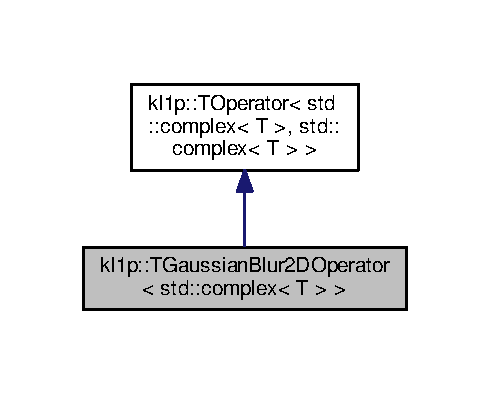
\includegraphics[width=235pt]{classkl1p_1_1TGaussianBlur2DOperator_3_01std_1_1complex_3_01T_01_4_01_4__inherit__graph}
\end{center}
\end{figure}


Collaboration diagram for kl1p\+:\+:T\+Gaussian\+Blur2\+D\+Operator$<$ std\+:\+:complex$<$ T $>$ $>$\+:
\nopagebreak
\begin{figure}[H]
\begin{center}
\leavevmode
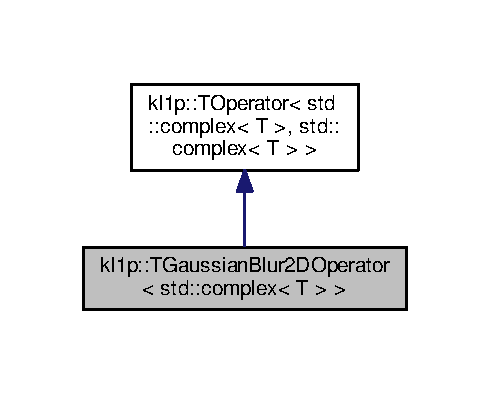
\includegraphics[width=235pt]{classkl1p_1_1TGaussianBlur2DOperator_3_01std_1_1complex_3_01T_01_4_01_4__coll__graph}
\end{center}
\end{figure}
\subsection*{Public Member Functions}
\begin{DoxyCompactItemize}
\item 
{\bfseries T\+Gaussian\+Blur2\+D\+Operator} (klab\+::\+U\+Int32 height, klab\+::\+U\+Int32 width)\hypertarget{classkl1p_1_1TGaussianBlur2DOperator_3_01std_1_1complex_3_01T_01_4_01_4_a0d117be68a934bb5ee2a3e9604121888}{}\label{classkl1p_1_1TGaussianBlur2DOperator_3_01std_1_1complex_3_01T_01_4_01_4_a0d117be68a934bb5ee2a3e9604121888}

\item 
{\bfseries T\+Gaussian\+Blur2\+D\+Operator} (klab\+::\+U\+Int32 height, klab\+::\+U\+Int32 width, const std\+::complex$<$ T $>$ \&sigma)\hypertarget{classkl1p_1_1TGaussianBlur2DOperator_3_01std_1_1complex_3_01T_01_4_01_4_a95ab38e138ba604ed217aa5a870635ec}{}\label{classkl1p_1_1TGaussianBlur2DOperator_3_01std_1_1complex_3_01T_01_4_01_4_a95ab38e138ba604ed217aa5a870635ec}

\item 
{\bfseries T\+Gaussian\+Blur2\+D\+Operator} (klab\+::\+U\+Int32 height, klab\+::\+U\+Int32 width, const std\+::complex$<$ T $>$ \&sigma, klab\+::\+Int32 ic, klab\+::\+Int32 jc)\hypertarget{classkl1p_1_1TGaussianBlur2DOperator_3_01std_1_1complex_3_01T_01_4_01_4_af4d4f9380d6b3f991031a62729be1795}{}\label{classkl1p_1_1TGaussianBlur2DOperator_3_01std_1_1complex_3_01T_01_4_01_4_af4d4f9380d6b3f991031a62729be1795}

\item 
{\bfseries T\+Gaussian\+Blur2\+D\+Operator} (const \hyperlink{classkl1p_1_1TGaussianBlur2DOperator}{T\+Gaussian\+Blur2\+D\+Operator}$<$ std\+::complex$<$ T $>$ $>$ \&op)\hypertarget{classkl1p_1_1TGaussianBlur2DOperator_3_01std_1_1complex_3_01T_01_4_01_4_a9e74aae2ca4e9ad24c7bb5d8aaf664f3}{}\label{classkl1p_1_1TGaussianBlur2DOperator_3_01std_1_1complex_3_01T_01_4_01_4_a9e74aae2ca4e9ad24c7bb5d8aaf664f3}

\item 
klab\+::\+U\+Int32 {\bfseries width} () const \hypertarget{classkl1p_1_1TGaussianBlur2DOperator_3_01std_1_1complex_3_01T_01_4_01_4_a3d0d32e3a06a8bcf73ff29966d6637a4}{}\label{classkl1p_1_1TGaussianBlur2DOperator_3_01std_1_1complex_3_01T_01_4_01_4_a3d0d32e3a06a8bcf73ff29966d6637a4}

\item 
klab\+::\+U\+Int32 {\bfseries height} () const \hypertarget{classkl1p_1_1TGaussianBlur2DOperator_3_01std_1_1complex_3_01T_01_4_01_4_aa7e9853f4098611cba1643a9cdd98150}{}\label{classkl1p_1_1TGaussianBlur2DOperator_3_01std_1_1complex_3_01T_01_4_01_4_aa7e9853f4098611cba1643a9cdd98150}

\item 
std\+::complex$<$ T $>$ {\bfseries sigma} () const \hypertarget{classkl1p_1_1TGaussianBlur2DOperator_3_01std_1_1complex_3_01T_01_4_01_4_a0e3c87084a5beed67a46b816b08979ce}{}\label{classkl1p_1_1TGaussianBlur2DOperator_3_01std_1_1complex_3_01T_01_4_01_4_a0e3c87084a5beed67a46b816b08979ce}

\item 
klab\+::\+Int32 {\bfseries ic} () const \hypertarget{classkl1p_1_1TGaussianBlur2DOperator_3_01std_1_1complex_3_01T_01_4_01_4_abf1f0c3187ddcff9c42496350113cee9}{}\label{classkl1p_1_1TGaussianBlur2DOperator_3_01std_1_1complex_3_01T_01_4_01_4_abf1f0c3187ddcff9c42496350113cee9}

\item 
klab\+::\+Int32 {\bfseries jc} () const \hypertarget{classkl1p_1_1TGaussianBlur2DOperator_3_01std_1_1complex_3_01T_01_4_01_4_abece5497f63a079327c3ccd63a0a5022}{}\label{classkl1p_1_1TGaussianBlur2DOperator_3_01std_1_1complex_3_01T_01_4_01_4_abece5497f63a079327c3ccd63a0a5022}

\item 
virtual void {\bfseries apply} (const arma\+::\+Col$<$ std\+::complex$<$ T $>$ $>$ \&in, arma\+::\+Col$<$ std\+::complex$<$ T $>$ $>$ \&out)\hypertarget{classkl1p_1_1TGaussianBlur2DOperator_3_01std_1_1complex_3_01T_01_4_01_4_af21db477a1af1c56132a1dc0988fbd75}{}\label{classkl1p_1_1TGaussianBlur2DOperator_3_01std_1_1complex_3_01T_01_4_01_4_af21db477a1af1c56132a1dc0988fbd75}

\item 
virtual void {\bfseries apply\+Adjoint} (const arma\+::\+Col$<$ std\+::complex$<$ T $>$ $>$ \&in, arma\+::\+Col$<$ std\+::complex$<$ T $>$ $>$ \&out)\hypertarget{classkl1p_1_1TGaussianBlur2DOperator_3_01std_1_1complex_3_01T_01_4_01_4_a329700e3a5f6b179b637850fbbb1cc2e}{}\label{classkl1p_1_1TGaussianBlur2DOperator_3_01std_1_1complex_3_01T_01_4_01_4_a329700e3a5f6b179b637850fbbb1cc2e}

\end{DoxyCompactItemize}
\subsection*{Additional Inherited Members}


The documentation for this class was generated from the following file\+:\begin{DoxyCompactItemize}
\item 
include/Gaussian\+Blur2\+D\+Operator.\+h\end{DoxyCompactItemize}

\hypertarget{classkl1p_1_1TGenericSeedingOperator}{}\section{kl1p\+:\+:T\+Generic\+Seeding\+Operator$<$ T, T\+Out, T\+Op $>$ Class Template Reference}
\label{classkl1p_1_1TGenericSeedingOperator}\index{kl1p\+::\+T\+Generic\+Seeding\+Operator$<$ T, T\+Out, T\+Op $>$@{kl1p\+::\+T\+Generic\+Seeding\+Operator$<$ T, T\+Out, T\+Op $>$}}


Inheritance diagram for kl1p\+:\+:T\+Generic\+Seeding\+Operator$<$ T, T\+Out, T\+Op $>$\+:
\nopagebreak
\begin{figure}[H]
\begin{center}
\leavevmode
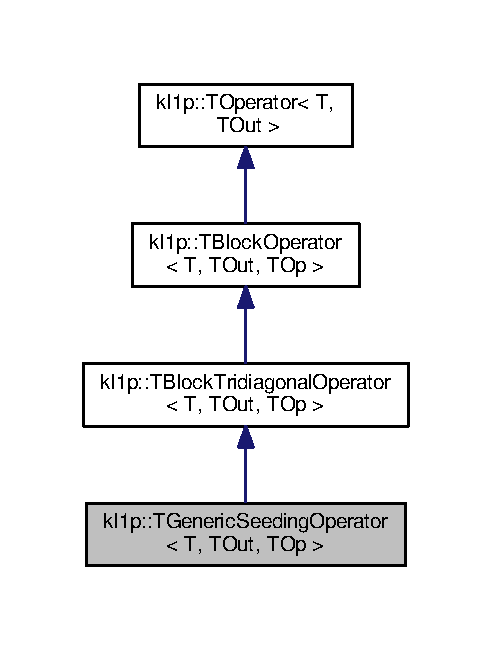
\includegraphics[width=236pt]{classkl1p_1_1TGenericSeedingOperator__inherit__graph}
\end{center}
\end{figure}


Collaboration diagram for kl1p\+:\+:T\+Generic\+Seeding\+Operator$<$ T, T\+Out, T\+Op $>$\+:
\nopagebreak
\begin{figure}[H]
\begin{center}
\leavevmode
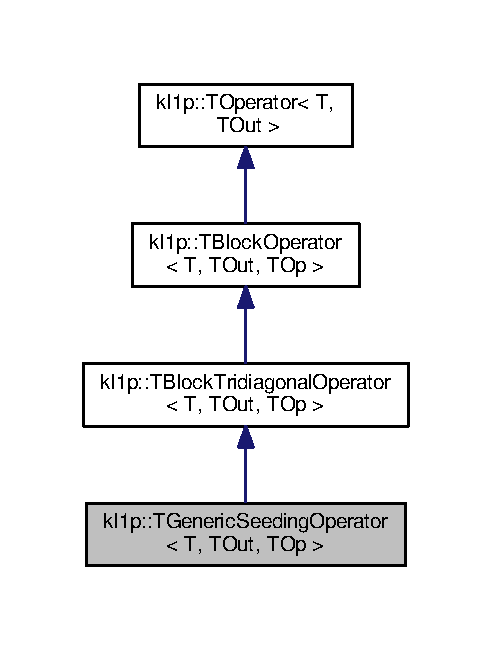
\includegraphics[width=236pt]{classkl1p_1_1TGenericSeedingOperator__coll__graph}
\end{center}
\end{figure}
\subsection*{Public Member Functions}
\begin{DoxyCompactItemize}
\item 
{\bfseries T\+Generic\+Seeding\+Operator} (klab\+::\+T\+Smart\+Pointer$<$ T\+Op $>$ op, klab\+::\+U\+Int32 blocks, klab\+::\+U\+Int32 m0, klab\+::\+U\+Int32 mb, const T \&diag\+Variance, const T \&lower\+Variance, const T \&upper\+Variance)\hypertarget{classkl1p_1_1TGenericSeedingOperator_aa42a0c840cc8ec6c7dca91218c84f0e2}{}\label{classkl1p_1_1TGenericSeedingOperator_aa42a0c840cc8ec6c7dca91218c84f0e2}

\item 
{\bfseries T\+Generic\+Seeding\+Operator} (const \hyperlink{classkl1p_1_1TGenericSeedingOperator}{T\+Generic\+Seeding\+Operator}$<$ T, T\+Out, T\+Op $>$ \&op)\hypertarget{classkl1p_1_1TGenericSeedingOperator_a9eb0b3dc73148533ad3c726bcdd14fb9}{}\label{classkl1p_1_1TGenericSeedingOperator_a9eb0b3dc73148533ad3c726bcdd14fb9}

\item 
klab\+::\+U\+Int32 {\bfseries count\+Seeded\+Blocks} () const \hypertarget{classkl1p_1_1TGenericSeedingOperator_a55030b751eeeaabe6559b37ff1f0f7ca}{}\label{classkl1p_1_1TGenericSeedingOperator_a55030b751eeeaabe6559b37ff1f0f7ca}

\item 
klab\+::\+U\+Int32 {\bfseries m0} () const \hypertarget{classkl1p_1_1TGenericSeedingOperator_ab4ca1833cb3d7cba6431f746fa1481e4}{}\label{classkl1p_1_1TGenericSeedingOperator_ab4ca1833cb3d7cba6431f746fa1481e4}

\item 
klab\+::\+U\+Int32 {\bfseries mb} () const \hypertarget{classkl1p_1_1TGenericSeedingOperator_a8847a788501a8f42f53a885e757ab347}{}\label{classkl1p_1_1TGenericSeedingOperator_a8847a788501a8f42f53a885e757ab347}

\item 
const T \& {\bfseries diagonal\+Variance} () const \hypertarget{classkl1p_1_1TGenericSeedingOperator_aa06d8cf54b856631f76192e67f31f906}{}\label{classkl1p_1_1TGenericSeedingOperator_aa06d8cf54b856631f76192e67f31f906}

\item 
const T \& {\bfseries lower\+Variance} () const \hypertarget{classkl1p_1_1TGenericSeedingOperator_a3532fe9c8ba76dd0cb26e6e3fe8108d8}{}\label{classkl1p_1_1TGenericSeedingOperator_a3532fe9c8ba76dd0cb26e6e3fe8108d8}

\item 
const T \& {\bfseries upper\+Variance} () const \hypertarget{classkl1p_1_1TGenericSeedingOperator_af5d552fd288a2fb36ea27412081440d4}{}\label{classkl1p_1_1TGenericSeedingOperator_af5d552fd288a2fb36ea27412081440d4}

\end{DoxyCompactItemize}
\subsection*{Protected Member Functions}
\begin{DoxyCompactItemize}
\item 
void {\bfseries init} (klab\+::\+T\+Smart\+Pointer$<$ T\+Op $>$ op, klab\+::\+U\+Int32 blocks, klab\+::\+U\+Int32 m0, klab\+::\+U\+Int32 mb, const T \&diag\+Variance, const T \&lower\+Variance, const T \&upper\+Variance)\hypertarget{classkl1p_1_1TGenericSeedingOperator_ab71f886e27c47e79de5561db5ada6174}{}\label{classkl1p_1_1TGenericSeedingOperator_ab71f886e27c47e79de5561db5ada6174}

\end{DoxyCompactItemize}
\subsection*{Additional Inherited Members}


The documentation for this class was generated from the following file\+:\begin{DoxyCompactItemize}
\item 
include/Generic\+Seeding\+Operator.\+h\end{DoxyCompactItemize}

\hypertarget{classkl1p_1_1TGenericSeedingOperatorSpecialisation}{}\section{kl1p\+:\+:T\+Generic\+Seeding\+Operator\+Specialisation$<$ T $>$ Class Template Reference}
\label{classkl1p_1_1TGenericSeedingOperatorSpecialisation}\index{kl1p\+::\+T\+Generic\+Seeding\+Operator\+Specialisation$<$ T $>$@{kl1p\+::\+T\+Generic\+Seeding\+Operator\+Specialisation$<$ T $>$}}
\subsection*{Static Public Member Functions}
\begin{DoxyCompactItemize}
\item 
static T {\bfseries Get\+Variance} (const T \&variance)\hypertarget{classkl1p_1_1TGenericSeedingOperatorSpecialisation_a2d58837b2e541ed8c4b7d5fe73c43b8b}{}\label{classkl1p_1_1TGenericSeedingOperatorSpecialisation_a2d58837b2e541ed8c4b7d5fe73c43b8b}

\end{DoxyCompactItemize}


The documentation for this class was generated from the following file\+:\begin{DoxyCompactItemize}
\item 
include/Generic\+Seeding\+Operator.\+h\end{DoxyCompactItemize}

\hypertarget{classkl1p_1_1TGenericSeedingOperatorSpecialisation_3_01std_1_1complex_3_01T_01_4_01_4}{}\section{kl1p\+:\+:T\+Generic\+Seeding\+Operator\+Specialisation$<$ std\+:\+:complex$<$ T $>$ $>$ Class Template Reference}
\label{classkl1p_1_1TGenericSeedingOperatorSpecialisation_3_01std_1_1complex_3_01T_01_4_01_4}\index{kl1p\+::\+T\+Generic\+Seeding\+Operator\+Specialisation$<$ std\+::complex$<$ T $>$ $>$@{kl1p\+::\+T\+Generic\+Seeding\+Operator\+Specialisation$<$ std\+::complex$<$ T $>$ $>$}}
\subsection*{Static Public Member Functions}
\begin{DoxyCompactItemize}
\item 
static std\+::complex$<$ T $>$ {\bfseries Get\+Variance} (const std\+::complex$<$ T $>$ \&variance)\hypertarget{classkl1p_1_1TGenericSeedingOperatorSpecialisation_3_01std_1_1complex_3_01T_01_4_01_4_a5deddec1470776af8e2da87e293d7558}{}\label{classkl1p_1_1TGenericSeedingOperatorSpecialisation_3_01std_1_1complex_3_01T_01_4_01_4_a5deddec1470776af8e2da87e293d7558}

\end{DoxyCompactItemize}


The documentation for this class was generated from the following file\+:\begin{DoxyCompactItemize}
\item 
include/Generic\+Seeding\+Operator.\+h\end{DoxyCompactItemize}

\hypertarget{classkl1p_1_1THistory}{}\section{kl1p\+:\+:T\+History$<$ T $>$ Class Template Reference}
\label{classkl1p_1_1THistory}\index{kl1p\+::\+T\+History$<$ T $>$@{kl1p\+::\+T\+History$<$ T $>$}}
\subsection*{Public Member Functions}
\begin{DoxyCompactItemize}
\item 
{\bfseries T\+History} (const \hyperlink{classkl1p_1_1THistory}{T\+History}$<$ T $>$ \&history)\hypertarget{classkl1p_1_1THistory_a044f45691a94a00aa01f1a1d87453f36}{}\label{classkl1p_1_1THistory_a044f45691a94a00aa01f1a1d87453f36}

\item 
\hyperlink{classkl1p_1_1THistory}{T\+History}$<$ T $>$ \& {\bfseries operator=} (const \hyperlink{classkl1p_1_1THistory}{T\+History}$<$ T $>$ \&history)\hypertarget{classkl1p_1_1THistory_aa0d9bde928573690d0c5f512f8db0a99}{}\label{classkl1p_1_1THistory_aa0d9bde928573690d0c5f512f8db0a99}

\item 
const T \& {\bfseries operator\mbox{[}$\,$\mbox{]}} (klab\+::\+U\+Int32 i) const \hypertarget{classkl1p_1_1THistory_ae6c5cdbfb60dfba396ab3ae0641b7a1a}{}\label{classkl1p_1_1THistory_ae6c5cdbfb60dfba396ab3ae0641b7a1a}

\item 
void {\bfseries clear} ()\hypertarget{classkl1p_1_1THistory_a6eedd4bc047d0f15c665b6c55061fb03}{}\label{classkl1p_1_1THistory_a6eedd4bc047d0f15c665b6c55061fb03}

\item 
void {\bfseries push} (const T \&element)\hypertarget{classkl1p_1_1THistory_a93644f4c1ae14036714da8c8a360cdf8}{}\label{classkl1p_1_1THistory_a93644f4c1ae14036714da8c8a360cdf8}

\item 
klab\+::\+U\+Int32 {\bfseries size} () const \hypertarget{classkl1p_1_1THistory_a05fa148ac119fce2cccf2935440fca10}{}\label{classkl1p_1_1THistory_a05fa148ac119fce2cccf2935440fca10}

\item 
const T \& {\bfseries element} (klab\+::\+U\+Int32 i) const \hypertarget{classkl1p_1_1THistory_a581351c161362ef7a02c4b799250f193}{}\label{classkl1p_1_1THistory_a581351c161362ef7a02c4b799250f193}

\end{DoxyCompactItemize}


The documentation for this class was generated from the following file\+:\begin{DoxyCompactItemize}
\item 
include/History.\+h\end{DoxyCompactItemize}

\hypertarget{classkl1p_1_1TIdentityOperator}{}\section{kl1p\+:\+:T\+Identity\+Operator$<$ T $>$ Class Template Reference}
\label{classkl1p_1_1TIdentityOperator}\index{kl1p\+::\+T\+Identity\+Operator$<$ T $>$@{kl1p\+::\+T\+Identity\+Operator$<$ T $>$}}


Inheritance diagram for kl1p\+:\+:T\+Identity\+Operator$<$ T $>$\+:
\nopagebreak
\begin{figure}[H]
\begin{center}
\leavevmode
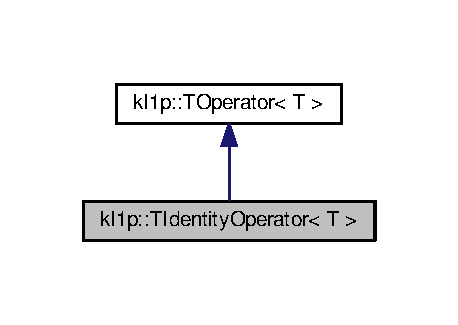
\includegraphics[width=220pt]{classkl1p_1_1TIdentityOperator__inherit__graph}
\end{center}
\end{figure}


Collaboration diagram for kl1p\+:\+:T\+Identity\+Operator$<$ T $>$\+:
\nopagebreak
\begin{figure}[H]
\begin{center}
\leavevmode
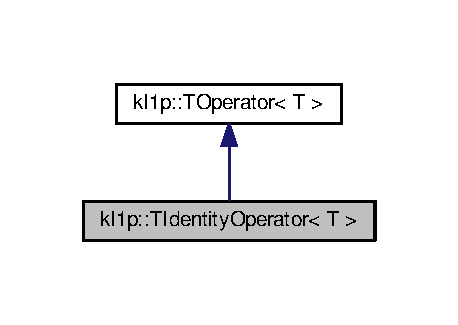
\includegraphics[width=220pt]{classkl1p_1_1TIdentityOperator__coll__graph}
\end{center}
\end{figure}
\subsection*{Public Member Functions}
\begin{DoxyCompactItemize}
\item 
{\bfseries T\+Identity\+Operator} (klab\+::\+U\+Int32 n)\hypertarget{classkl1p_1_1TIdentityOperator_a9034d91ead0141c4cb1f13c7b5eee75f}{}\label{classkl1p_1_1TIdentityOperator_a9034d91ead0141c4cb1f13c7b5eee75f}

\item 
{\bfseries T\+Identity\+Operator} (const \hyperlink{classkl1p_1_1TIdentityOperator}{T\+Identity\+Operator}$<$ T $>$ \&op)\hypertarget{classkl1p_1_1TIdentityOperator_a7f74406ba363d22647558c53af95dfb6}{}\label{classkl1p_1_1TIdentityOperator_a7f74406ba363d22647558c53af95dfb6}

\item 
virtual void {\bfseries apply} (const arma\+::\+Col$<$ T $>$ \&in, arma\+::\+Col$<$ T $>$ \&out)\hypertarget{classkl1p_1_1TIdentityOperator_ad0b77a8e0b1b3cd7ef38fab2565b2ac2}{}\label{classkl1p_1_1TIdentityOperator_ad0b77a8e0b1b3cd7ef38fab2565b2ac2}

\item 
virtual void {\bfseries apply\+Adjoint} (const arma\+::\+Col$<$ T $>$ \&in, arma\+::\+Col$<$ T $>$ \&out)\hypertarget{classkl1p_1_1TIdentityOperator_a9a7423f97c68bf7b5b6945f176638ecd}{}\label{classkl1p_1_1TIdentityOperator_a9a7423f97c68bf7b5b6945f176638ecd}

\item 
virtual void {\bfseries column} (klab\+::\+U\+Int32 i, arma\+::\+Col$<$ T $>$ \&out)\hypertarget{classkl1p_1_1TIdentityOperator_a2b5f3144ce1d48e2c76d415ccc587d3c}{}\label{classkl1p_1_1TIdentityOperator_a2b5f3144ce1d48e2c76d415ccc587d3c}

\item 
virtual void {\bfseries column\+Adjoint} (klab\+::\+U\+Int32 i, arma\+::\+Col$<$ T $>$ \&out)\hypertarget{classkl1p_1_1TIdentityOperator_af87877f80e4fe2abc6c5952839316eb7}{}\label{classkl1p_1_1TIdentityOperator_af87877f80e4fe2abc6c5952839316eb7}

\end{DoxyCompactItemize}
\subsection*{Additional Inherited Members}


The documentation for this class was generated from the following file\+:\begin{DoxyCompactItemize}
\item 
include/Identity\+Operator.\+h\end{DoxyCompactItemize}

\hypertarget{classkl1p_1_1TInverseDCT1DOperator}{}\section{kl1p\+:\+:T\+Inverse\+D\+C\+T1\+D\+Operator$<$ T $>$ Class Template Reference}
\label{classkl1p_1_1TInverseDCT1DOperator}\index{kl1p\+::\+T\+Inverse\+D\+C\+T1\+D\+Operator$<$ T $>$@{kl1p\+::\+T\+Inverse\+D\+C\+T1\+D\+Operator$<$ T $>$}}


Inheritance diagram for kl1p\+:\+:T\+Inverse\+D\+C\+T1\+D\+Operator$<$ T $>$\+:
\nopagebreak
\begin{figure}[H]
\begin{center}
\leavevmode
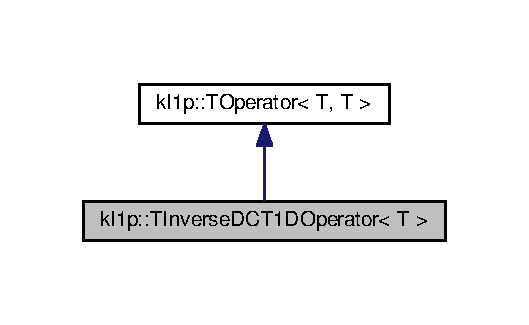
\includegraphics[width=254pt]{classkl1p_1_1TInverseDCT1DOperator__inherit__graph}
\end{center}
\end{figure}


Collaboration diagram for kl1p\+:\+:T\+Inverse\+D\+C\+T1\+D\+Operator$<$ T $>$\+:
\nopagebreak
\begin{figure}[H]
\begin{center}
\leavevmode
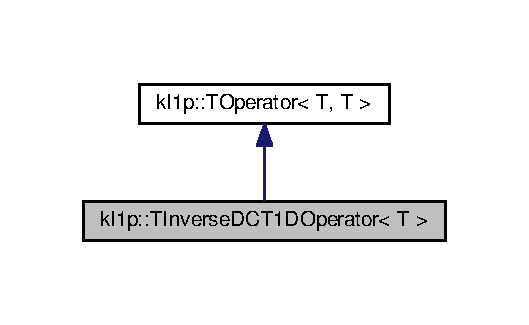
\includegraphics[width=254pt]{classkl1p_1_1TInverseDCT1DOperator__coll__graph}
\end{center}
\end{figure}
\subsection*{Public Member Functions}
\begin{DoxyCompactItemize}
\item 
{\bfseries T\+Inverse\+D\+C\+T1\+D\+Operator} (klab\+::\+U\+Int32 n)\hypertarget{classkl1p_1_1TInverseDCT1DOperator_afa81febe834685376d6d7c043a1faf08}{}\label{classkl1p_1_1TInverseDCT1DOperator_afa81febe834685376d6d7c043a1faf08}

\item 
{\bfseries T\+Inverse\+D\+C\+T1\+D\+Operator} (const \hyperlink{classkl1p_1_1TInverseDCT1DOperator}{T\+Inverse\+D\+C\+T1\+D\+Operator}$<$ T $>$ \&op)\hypertarget{classkl1p_1_1TInverseDCT1DOperator_aaadd54b7ea9f6e36e18317fbf7e1dc72}{}\label{classkl1p_1_1TInverseDCT1DOperator_aaadd54b7ea9f6e36e18317fbf7e1dc72}

\item 
virtual void {\bfseries apply} (const arma\+::\+Col$<$ T $>$ \&in, arma\+::\+Col$<$ T $>$ \&out)\hypertarget{classkl1p_1_1TInverseDCT1DOperator_a06a902a7a249649d0a1a253c3528822e}{}\label{classkl1p_1_1TInverseDCT1DOperator_a06a902a7a249649d0a1a253c3528822e}

\item 
virtual void {\bfseries apply\+Adjoint} (const arma\+::\+Col$<$ T $>$ \&in, arma\+::\+Col$<$ T $>$ \&out)\hypertarget{classkl1p_1_1TInverseDCT1DOperator_af6f98150c3844a749a326b57367c1e45}{}\label{classkl1p_1_1TInverseDCT1DOperator_af6f98150c3844a749a326b57367c1e45}

\end{DoxyCompactItemize}
\subsection*{Additional Inherited Members}


The documentation for this class was generated from the following file\+:\begin{DoxyCompactItemize}
\item 
include/Inverse\+D\+C\+T1\+D\+Operator.\+h\end{DoxyCompactItemize}

\hypertarget{classkl1p_1_1TInverseDCT2DOperator}{}\section{kl1p\+:\+:T\+Inverse\+D\+C\+T2\+D\+Operator$<$ T $>$ Class Template Reference}
\label{classkl1p_1_1TInverseDCT2DOperator}\index{kl1p\+::\+T\+Inverse\+D\+C\+T2\+D\+Operator$<$ T $>$@{kl1p\+::\+T\+Inverse\+D\+C\+T2\+D\+Operator$<$ T $>$}}


Inheritance diagram for kl1p\+:\+:T\+Inverse\+D\+C\+T2\+D\+Operator$<$ T $>$\+:
\nopagebreak
\begin{figure}[H]
\begin{center}
\leavevmode
\includegraphics[width=254pt]{classkl1p_1_1TInverseDCT2DOperator__inherit__graph}
\end{center}
\end{figure}


Collaboration diagram for kl1p\+:\+:T\+Inverse\+D\+C\+T2\+D\+Operator$<$ T $>$\+:
\nopagebreak
\begin{figure}[H]
\begin{center}
\leavevmode
\includegraphics[width=254pt]{classkl1p_1_1TInverseDCT2DOperator__coll__graph}
\end{center}
\end{figure}
\subsection*{Public Member Functions}
\begin{DoxyCompactItemize}
\item 
{\bfseries T\+Inverse\+D\+C\+T2\+D\+Operator} (klab\+::\+U\+Int32 height, klab\+::\+U\+Int32 width)\hypertarget{classkl1p_1_1TInverseDCT2DOperator_ac39838e9d518ceb63e306b2e09c2bf04}{}\label{classkl1p_1_1TInverseDCT2DOperator_ac39838e9d518ceb63e306b2e09c2bf04}

\item 
{\bfseries T\+Inverse\+D\+C\+T2\+D\+Operator} (const \hyperlink{classkl1p_1_1TInverseDCT2DOperator}{T\+Inverse\+D\+C\+T2\+D\+Operator}$<$ T $>$ \&op)\hypertarget{classkl1p_1_1TInverseDCT2DOperator_a3a018c10d261c4cc7cef641539cae2b3}{}\label{classkl1p_1_1TInverseDCT2DOperator_a3a018c10d261c4cc7cef641539cae2b3}

\item 
klab\+::\+U\+Int32 {\bfseries width} () const \hypertarget{classkl1p_1_1TInverseDCT2DOperator_a043e67af346e4cf08352ac206359f001}{}\label{classkl1p_1_1TInverseDCT2DOperator_a043e67af346e4cf08352ac206359f001}

\item 
klab\+::\+U\+Int32 {\bfseries height} () const \hypertarget{classkl1p_1_1TInverseDCT2DOperator_adcd32ec5f34b0729233f83409fc4a777}{}\label{classkl1p_1_1TInverseDCT2DOperator_adcd32ec5f34b0729233f83409fc4a777}

\item 
virtual void {\bfseries apply} (const arma\+::\+Col$<$ T $>$ \&in, arma\+::\+Col$<$ T $>$ \&out)\hypertarget{classkl1p_1_1TInverseDCT2DOperator_a4a97e8344c8a510ffe795b8715ab136c}{}\label{classkl1p_1_1TInverseDCT2DOperator_a4a97e8344c8a510ffe795b8715ab136c}

\item 
virtual void {\bfseries apply\+Adjoint} (const arma\+::\+Col$<$ T $>$ \&in, arma\+::\+Col$<$ T $>$ \&out)\hypertarget{classkl1p_1_1TInverseDCT2DOperator_aa06aa031800e430226129c37f2848687}{}\label{classkl1p_1_1TInverseDCT2DOperator_aa06aa031800e430226129c37f2848687}

\end{DoxyCompactItemize}
\subsection*{Additional Inherited Members}


The documentation for this class was generated from the following file\+:\begin{DoxyCompactItemize}
\item 
include/Inverse\+D\+C\+T2\+D\+Operator.\+h\end{DoxyCompactItemize}

\hypertarget{classkl1p_1_1TInverseFourier1DOperator}{}\section{kl1p\+:\+:T\+Inverse\+Fourier1\+D\+Operator$<$ T $>$ Class Template Reference}
\label{classkl1p_1_1TInverseFourier1DOperator}\index{kl1p\+::\+T\+Inverse\+Fourier1\+D\+Operator$<$ T $>$@{kl1p\+::\+T\+Inverse\+Fourier1\+D\+Operator$<$ T $>$}}


Inheritance diagram for kl1p\+:\+:T\+Inverse\+Fourier1\+D\+Operator$<$ T $>$\+:
\nopagebreak
\begin{figure}[H]
\begin{center}
\leavevmode
\includegraphics[width=263pt]{classkl1p_1_1TInverseFourier1DOperator__inherit__graph}
\end{center}
\end{figure}


Collaboration diagram for kl1p\+:\+:T\+Inverse\+Fourier1\+D\+Operator$<$ T $>$\+:
\nopagebreak
\begin{figure}[H]
\begin{center}
\leavevmode
\includegraphics[width=263pt]{classkl1p_1_1TInverseFourier1DOperator__coll__graph}
\end{center}
\end{figure}
\subsection*{Public Member Functions}
\begin{DoxyCompactItemize}
\item 
{\bfseries T\+Inverse\+Fourier1\+D\+Operator} (klab\+::\+U\+Int32 n)\hypertarget{classkl1p_1_1TInverseFourier1DOperator_a8eda1becaf73544501373c7b0a8f19bc}{}\label{classkl1p_1_1TInverseFourier1DOperator_a8eda1becaf73544501373c7b0a8f19bc}

\item 
{\bfseries T\+Inverse\+Fourier1\+D\+Operator} (klab\+::\+U\+Int32 n, bool shift)\hypertarget{classkl1p_1_1TInverseFourier1DOperator_abc24332387f8bc11f861457038d310ce}{}\label{classkl1p_1_1TInverseFourier1DOperator_abc24332387f8bc11f861457038d310ce}

\item 
{\bfseries T\+Inverse\+Fourier1\+D\+Operator} (const \hyperlink{classkl1p_1_1TInverseFourier1DOperator}{T\+Inverse\+Fourier1\+D\+Operator}$<$ T $>$ \&op)\hypertarget{classkl1p_1_1TInverseFourier1DOperator_a5c021cbe2c2e6bd3402400b2fa3641c4}{}\label{classkl1p_1_1TInverseFourier1DOperator_a5c021cbe2c2e6bd3402400b2fa3641c4}

\item 
bool {\bfseries is\+Shift} () const \hypertarget{classkl1p_1_1TInverseFourier1DOperator_a2b8e98045c1970d837dc7d875e134c59}{}\label{classkl1p_1_1TInverseFourier1DOperator_a2b8e98045c1970d837dc7d875e134c59}

\item 
virtual void {\bfseries apply} (const arma\+::\+Col$<$ T $>$ \&in, arma\+::\+Col$<$ T $>$ \&out)\hypertarget{classkl1p_1_1TInverseFourier1DOperator_a52a7a76d8e77c90ff9b57f5a4472e746}{}\label{classkl1p_1_1TInverseFourier1DOperator_a52a7a76d8e77c90ff9b57f5a4472e746}

\item 
virtual void {\bfseries apply\+Adjoint} (const arma\+::\+Col$<$ T $>$ \&in, arma\+::\+Col$<$ T $>$ \&out)\hypertarget{classkl1p_1_1TInverseFourier1DOperator_aea796462cfa5a9074d37df9c7b2217de}{}\label{classkl1p_1_1TInverseFourier1DOperator_aea796462cfa5a9074d37df9c7b2217de}

\end{DoxyCompactItemize}
\subsection*{Additional Inherited Members}


The documentation for this class was generated from the following file\+:\begin{DoxyCompactItemize}
\item 
include/Inverse\+Fourier1\+D\+Operator.\+h\end{DoxyCompactItemize}

\hypertarget{classkl1p_1_1TInverseFourier1DOperatorSpecialisation}{}\section{kl1p\+:\+:T\+Inverse\+Fourier1\+D\+Operator\+Specialisation$<$ T $>$ Class Template Reference}
\label{classkl1p_1_1TInverseFourier1DOperatorSpecialisation}\index{kl1p\+::\+T\+Inverse\+Fourier1\+D\+Operator\+Specialisation$<$ T $>$@{kl1p\+::\+T\+Inverse\+Fourier1\+D\+Operator\+Specialisation$<$ T $>$}}
\subsection*{Static Public Member Functions}
\begin{DoxyCompactItemize}
\item 
static void {\bfseries Apply\+Adjoint} (const arma\+::\+Col$<$ T $>$ \&in, arma\+::\+Col$<$ T $>$ \&out, klab\+::\+T\+F\+F\+T1D$<$ T $>$ \&fft)\hypertarget{classkl1p_1_1TInverseFourier1DOperatorSpecialisation_aa9dea9b7f88a1f6a51f485d778de0544}{}\label{classkl1p_1_1TInverseFourier1DOperatorSpecialisation_aa9dea9b7f88a1f6a51f485d778de0544}

\end{DoxyCompactItemize}


The documentation for this class was generated from the following file\+:\begin{DoxyCompactItemize}
\item 
include/Inverse\+Fourier1\+D\+Operator.\+h\end{DoxyCompactItemize}

\hypertarget{classkl1p_1_1TInverseFourier1DOperatorSpecialisation_3_01std_1_1complex_3_01T_01_4_01_4}{}\section{kl1p\+:\+:T\+Inverse\+Fourier1\+D\+Operator\+Specialisation$<$ std\+:\+:complex$<$ T $>$ $>$ Class Template Reference}
\label{classkl1p_1_1TInverseFourier1DOperatorSpecialisation_3_01std_1_1complex_3_01T_01_4_01_4}\index{kl1p\+::\+T\+Inverse\+Fourier1\+D\+Operator\+Specialisation$<$ std\+::complex$<$ T $>$ $>$@{kl1p\+::\+T\+Inverse\+Fourier1\+D\+Operator\+Specialisation$<$ std\+::complex$<$ T $>$ $>$}}
\subsection*{Static Public Member Functions}
\begin{DoxyCompactItemize}
\item 
static void {\bfseries Apply\+Adjoint} (const arma\+::\+Col$<$ std\+::complex$<$ T $>$ $>$ \&in, arma\+::\+Col$<$ std\+::complex$<$ T $>$ $>$ \&out, klab\+::\+T\+F\+F\+T1D$<$ std\+::complex$<$ T $>$ $>$ \&fft)\hypertarget{classkl1p_1_1TInverseFourier1DOperatorSpecialisation_3_01std_1_1complex_3_01T_01_4_01_4_a7b996419815adcd6b676319e700e7018}{}\label{classkl1p_1_1TInverseFourier1DOperatorSpecialisation_3_01std_1_1complex_3_01T_01_4_01_4_a7b996419815adcd6b676319e700e7018}

\end{DoxyCompactItemize}


The documentation for this class was generated from the following file\+:\begin{DoxyCompactItemize}
\item 
include/Inverse\+Fourier1\+D\+Operator.\+h\end{DoxyCompactItemize}

\hypertarget{classkl1p_1_1TInverseFourier2DOperator}{}\section{kl1p\+:\+:T\+Inverse\+Fourier2\+D\+Operator$<$ T $>$ Class Template Reference}
\label{classkl1p_1_1TInverseFourier2DOperator}\index{kl1p\+::\+T\+Inverse\+Fourier2\+D\+Operator$<$ T $>$@{kl1p\+::\+T\+Inverse\+Fourier2\+D\+Operator$<$ T $>$}}


Inheritance diagram for kl1p\+:\+:T\+Inverse\+Fourier2\+D\+Operator$<$ T $>$\+:
\nopagebreak
\begin{figure}[H]
\begin{center}
\leavevmode
\includegraphics[width=263pt]{classkl1p_1_1TInverseFourier2DOperator__inherit__graph}
\end{center}
\end{figure}


Collaboration diagram for kl1p\+:\+:T\+Inverse\+Fourier2\+D\+Operator$<$ T $>$\+:
\nopagebreak
\begin{figure}[H]
\begin{center}
\leavevmode
\includegraphics[width=263pt]{classkl1p_1_1TInverseFourier2DOperator__coll__graph}
\end{center}
\end{figure}
\subsection*{Public Member Functions}
\begin{DoxyCompactItemize}
\item 
{\bfseries T\+Inverse\+Fourier2\+D\+Operator} (klab\+::\+U\+Int32 height, klab\+::\+U\+Int32 width, bool shift=false)\hypertarget{classkl1p_1_1TInverseFourier2DOperator_a82eb1802681b2e93d7ff9f770087a6b1}{}\label{classkl1p_1_1TInverseFourier2DOperator_a82eb1802681b2e93d7ff9f770087a6b1}

\item 
{\bfseries T\+Inverse\+Fourier2\+D\+Operator} (const \hyperlink{classkl1p_1_1TInverseFourier2DOperator}{T\+Inverse\+Fourier2\+D\+Operator}$<$ T $>$ \&op)\hypertarget{classkl1p_1_1TInverseFourier2DOperator_a62049a21074fe238e4a568de03537ee2}{}\label{classkl1p_1_1TInverseFourier2DOperator_a62049a21074fe238e4a568de03537ee2}

\item 
klab\+::\+U\+Int32 {\bfseries width} () const \hypertarget{classkl1p_1_1TInverseFourier2DOperator_aebf7160bfe28b5f366a3694ad6981df9}{}\label{classkl1p_1_1TInverseFourier2DOperator_aebf7160bfe28b5f366a3694ad6981df9}

\item 
klab\+::\+U\+Int32 {\bfseries height} () const \hypertarget{classkl1p_1_1TInverseFourier2DOperator_a3e73c70b4d9aa0b6332d13dc6106145f}{}\label{classkl1p_1_1TInverseFourier2DOperator_a3e73c70b4d9aa0b6332d13dc6106145f}

\item 
bool {\bfseries is\+Shift} () const \hypertarget{classkl1p_1_1TInverseFourier2DOperator_afaaf34a0c7a461571902b793465526af}{}\label{classkl1p_1_1TInverseFourier2DOperator_afaaf34a0c7a461571902b793465526af}

\item 
virtual void {\bfseries apply} (const arma\+::\+Col$<$ T $>$ \&in, arma\+::\+Col$<$ T $>$ \&out)\hypertarget{classkl1p_1_1TInverseFourier2DOperator_a85597bcec3dfb26961d8440a0474c6e8}{}\label{classkl1p_1_1TInverseFourier2DOperator_a85597bcec3dfb26961d8440a0474c6e8}

\item 
virtual void {\bfseries apply\+Adjoint} (const arma\+::\+Col$<$ T $>$ \&in, arma\+::\+Col$<$ T $>$ \&out)\hypertarget{classkl1p_1_1TInverseFourier2DOperator_ac0647122ff006e614302eee9096e3704}{}\label{classkl1p_1_1TInverseFourier2DOperator_ac0647122ff006e614302eee9096e3704}

\end{DoxyCompactItemize}
\subsection*{Additional Inherited Members}


The documentation for this class was generated from the following file\+:\begin{DoxyCompactItemize}
\item 
include/Inverse\+Fourier2\+D\+Operator.\+h\end{DoxyCompactItemize}

\hypertarget{classkl1p_1_1TInverseFourier2DOperatorSpecialisation}{}\section{kl1p\+:\+:T\+Inverse\+Fourier2\+D\+Operator\+Specialisation$<$ T $>$ Class Template Reference}
\label{classkl1p_1_1TInverseFourier2DOperatorSpecialisation}\index{kl1p\+::\+T\+Inverse\+Fourier2\+D\+Operator\+Specialisation$<$ T $>$@{kl1p\+::\+T\+Inverse\+Fourier2\+D\+Operator\+Specialisation$<$ T $>$}}
\subsection*{Static Public Member Functions}
\begin{DoxyCompactItemize}
\item 
static void {\bfseries Apply\+Adjoint} (const arma\+::\+Col$<$ T $>$ \&in, arma\+::\+Col$<$ T $>$ \&out, klab\+::\+U\+Int32 height, klab\+::\+U\+Int32 width, klab\+::\+T\+F\+F\+T2D$<$ T $>$ \&fft)\hypertarget{classkl1p_1_1TInverseFourier2DOperatorSpecialisation_a4ae294c57334c18d651ebedc8f3b19d0}{}\label{classkl1p_1_1TInverseFourier2DOperatorSpecialisation_a4ae294c57334c18d651ebedc8f3b19d0}

\end{DoxyCompactItemize}
\subsection*{Static Protected Member Functions}
\begin{DoxyCompactItemize}
\item 
static void {\bfseries Apply\+Adjoint\+To\+Matrix\+Columns} (const arma\+::\+Mat$<$ T $>$ \&in, arma\+::\+Mat$<$ T $>$ \&out, klab\+::\+T\+F\+F\+T1D$<$ T $>$ \&fft)\hypertarget{classkl1p_1_1TInverseFourier2DOperatorSpecialisation_ab1f8ced247b7ec1e5ae55ec2bf6519da}{}\label{classkl1p_1_1TInverseFourier2DOperatorSpecialisation_ab1f8ced247b7ec1e5ae55ec2bf6519da}

\end{DoxyCompactItemize}


The documentation for this class was generated from the following file\+:\begin{DoxyCompactItemize}
\item 
include/Inverse\+Fourier2\+D\+Operator.\+h\end{DoxyCompactItemize}

\hypertarget{classkl1p_1_1TInverseFourier2DOperatorSpecialisation_3_01std_1_1complex_3_01T_01_4_01_4}{}\section{kl1p\+:\+:T\+Inverse\+Fourier2\+D\+Operator\+Specialisation$<$ std\+:\+:complex$<$ T $>$ $>$ Class Template Reference}
\label{classkl1p_1_1TInverseFourier2DOperatorSpecialisation_3_01std_1_1complex_3_01T_01_4_01_4}\index{kl1p\+::\+T\+Inverse\+Fourier2\+D\+Operator\+Specialisation$<$ std\+::complex$<$ T $>$ $>$@{kl1p\+::\+T\+Inverse\+Fourier2\+D\+Operator\+Specialisation$<$ std\+::complex$<$ T $>$ $>$}}
\subsection*{Static Public Member Functions}
\begin{DoxyCompactItemize}
\item 
static void {\bfseries Apply\+Adjoint} (const arma\+::\+Col$<$ std\+::complex$<$ T $>$ $>$ \&in, arma\+::\+Col$<$ std\+::complex$<$ T $>$ $>$ \&out, klab\+::\+U\+Int32 height, klab\+::\+U\+Int32 width, klab\+::\+T\+F\+F\+T2D$<$ std\+::complex$<$ T $>$ $>$ \&fft)\hypertarget{classkl1p_1_1TInverseFourier2DOperatorSpecialisation_3_01std_1_1complex_3_01T_01_4_01_4_ae7996f0948e920df52340215719eff1c}{}\label{classkl1p_1_1TInverseFourier2DOperatorSpecialisation_3_01std_1_1complex_3_01T_01_4_01_4_ae7996f0948e920df52340215719eff1c}

\end{DoxyCompactItemize}


The documentation for this class was generated from the following file\+:\begin{DoxyCompactItemize}
\item 
include/Inverse\+Fourier2\+D\+Operator.\+h\end{DoxyCompactItemize}

\hypertarget{classkl1p_1_1TInverseGaussian1DDiagonalOperator}{}\section{kl1p\+:\+:T\+Inverse\+Gaussian1\+D\+Diagonal\+Operator$<$ T $>$ Class Template Reference}
\label{classkl1p_1_1TInverseGaussian1DDiagonalOperator}\index{kl1p\+::\+T\+Inverse\+Gaussian1\+D\+Diagonal\+Operator$<$ T $>$@{kl1p\+::\+T\+Inverse\+Gaussian1\+D\+Diagonal\+Operator$<$ T $>$}}


Inheritance diagram for kl1p\+:\+:T\+Inverse\+Gaussian1\+D\+Diagonal\+Operator$<$ T $>$\+:
\nopagebreak
\begin{figure}[H]
\begin{center}
\leavevmode
\includegraphics[width=251pt]{classkl1p_1_1TInverseGaussian1DDiagonalOperator__inherit__graph}
\end{center}
\end{figure}


Collaboration diagram for kl1p\+:\+:T\+Inverse\+Gaussian1\+D\+Diagonal\+Operator$<$ T $>$\+:
\nopagebreak
\begin{figure}[H]
\begin{center}
\leavevmode
\includegraphics[width=251pt]{classkl1p_1_1TInverseGaussian1DDiagonalOperator__coll__graph}
\end{center}
\end{figure}
\subsection*{Public Member Functions}
\begin{DoxyCompactItemize}
\item 
{\bfseries T\+Inverse\+Gaussian1\+D\+Diagonal\+Operator} (klab\+::\+U\+Int32 n)\hypertarget{classkl1p_1_1TInverseGaussian1DDiagonalOperator_a10197a1746d41e8ff957d65139e67af8}{}\label{classkl1p_1_1TInverseGaussian1DDiagonalOperator_a10197a1746d41e8ff957d65139e67af8}

\item 
{\bfseries T\+Inverse\+Gaussian1\+D\+Diagonal\+Operator} (klab\+::\+U\+Int32 n, const T \&gamma)\hypertarget{classkl1p_1_1TInverseGaussian1DDiagonalOperator_afe9227318fadd3ac49e5665bb5dfef32}{}\label{classkl1p_1_1TInverseGaussian1DDiagonalOperator_afe9227318fadd3ac49e5665bb5dfef32}

\item 
{\bfseries T\+Inverse\+Gaussian1\+D\+Diagonal\+Operator} (klab\+::\+U\+Int32 n, const T \&gamma, const T \&sigma)\hypertarget{classkl1p_1_1TInverseGaussian1DDiagonalOperator_ac7a56fee4545554a61bb3a10d8dde337}{}\label{classkl1p_1_1TInverseGaussian1DDiagonalOperator_ac7a56fee4545554a61bb3a10d8dde337}

\item 
{\bfseries T\+Inverse\+Gaussian1\+D\+Diagonal\+Operator} (klab\+::\+U\+Int32 n, const T \&gamma, const T \&sigma, klab\+::\+Int32 c)\hypertarget{classkl1p_1_1TInverseGaussian1DDiagonalOperator_ab70236c84c478492a015e8e61473108d}{}\label{classkl1p_1_1TInverseGaussian1DDiagonalOperator_ab70236c84c478492a015e8e61473108d}

\item 
{\bfseries T\+Inverse\+Gaussian1\+D\+Diagonal\+Operator} (const \hyperlink{classkl1p_1_1TInverseGaussian1DDiagonalOperator}{T\+Inverse\+Gaussian1\+D\+Diagonal\+Operator}$<$ T $>$ \&op)\hypertarget{classkl1p_1_1TInverseGaussian1DDiagonalOperator_a1db8296778ef61e2510edd16e96ad821}{}\label{classkl1p_1_1TInverseGaussian1DDiagonalOperator_a1db8296778ef61e2510edd16e96ad821}

\item 
const T \& {\bfseries gamma} () const \hypertarget{classkl1p_1_1TInverseGaussian1DDiagonalOperator_ad204508c60be12f8203809a5b4e102cc}{}\label{classkl1p_1_1TInverseGaussian1DDiagonalOperator_ad204508c60be12f8203809a5b4e102cc}

\item 
const T \& {\bfseries sigma} () const \hypertarget{classkl1p_1_1TInverseGaussian1DDiagonalOperator_a97a84c4fb5f03752bd414169e4b6f411}{}\label{classkl1p_1_1TInverseGaussian1DDiagonalOperator_a97a84c4fb5f03752bd414169e4b6f411}

\item 
klab\+::\+Int32 {\bfseries c} () const \hypertarget{classkl1p_1_1TInverseGaussian1DDiagonalOperator_aa0447d8b688d848d93898fb452cf30e8}{}\label{classkl1p_1_1TInverseGaussian1DDiagonalOperator_aa0447d8b688d848d93898fb452cf30e8}

\end{DoxyCompactItemize}
\subsection*{Additional Inherited Members}


The documentation for this class was generated from the following file\+:\begin{DoxyCompactItemize}
\item 
include/Inverse\+Gaussian1\+D\+Diagonal\+Operator.\+h\end{DoxyCompactItemize}

\hypertarget{classkl1p_1_1TInverseGaussian2DDiagonalOperator}{}\section{kl1p\+:\+:T\+Inverse\+Gaussian2\+D\+Diagonal\+Operator$<$ T $>$ Class Template Reference}
\label{classkl1p_1_1TInverseGaussian2DDiagonalOperator}\index{kl1p\+::\+T\+Inverse\+Gaussian2\+D\+Diagonal\+Operator$<$ T $>$@{kl1p\+::\+T\+Inverse\+Gaussian2\+D\+Diagonal\+Operator$<$ T $>$}}


Inheritance diagram for kl1p\+:\+:T\+Inverse\+Gaussian2\+D\+Diagonal\+Operator$<$ T $>$\+:
\nopagebreak
\begin{figure}[H]
\begin{center}
\leavevmode
\includegraphics[width=251pt]{classkl1p_1_1TInverseGaussian2DDiagonalOperator__inherit__graph}
\end{center}
\end{figure}


Collaboration diagram for kl1p\+:\+:T\+Inverse\+Gaussian2\+D\+Diagonal\+Operator$<$ T $>$\+:
\nopagebreak
\begin{figure}[H]
\begin{center}
\leavevmode
\includegraphics[width=251pt]{classkl1p_1_1TInverseGaussian2DDiagonalOperator__coll__graph}
\end{center}
\end{figure}
\subsection*{Public Member Functions}
\begin{DoxyCompactItemize}
\item 
{\bfseries T\+Inverse\+Gaussian2\+D\+Diagonal\+Operator} (klab\+::\+U\+Int32 height, klab\+::\+U\+Int32 width)\hypertarget{classkl1p_1_1TInverseGaussian2DDiagonalOperator_ad5281d2c861d9613800a0fcfd49fa7ca}{}\label{classkl1p_1_1TInverseGaussian2DDiagonalOperator_ad5281d2c861d9613800a0fcfd49fa7ca}

\item 
{\bfseries T\+Inverse\+Gaussian2\+D\+Diagonal\+Operator} (klab\+::\+U\+Int32 height, klab\+::\+U\+Int32 width, const T \&gamma)\hypertarget{classkl1p_1_1TInverseGaussian2DDiagonalOperator_a0c9eb6d9de01585397f0015750921d00}{}\label{classkl1p_1_1TInverseGaussian2DDiagonalOperator_a0c9eb6d9de01585397f0015750921d00}

\item 
{\bfseries T\+Inverse\+Gaussian2\+D\+Diagonal\+Operator} (klab\+::\+U\+Int32 height, klab\+::\+U\+Int32 width, const T \&gamma, const T \&sigma)\hypertarget{classkl1p_1_1TInverseGaussian2DDiagonalOperator_a717270cb5bfabd1f42d3980be693e788}{}\label{classkl1p_1_1TInverseGaussian2DDiagonalOperator_a717270cb5bfabd1f42d3980be693e788}

\item 
{\bfseries T\+Inverse\+Gaussian2\+D\+Diagonal\+Operator} (klab\+::\+U\+Int32 height, klab\+::\+U\+Int32 width, const T \&gamma, const T \&sigma, klab\+::\+Int32 ic, klab\+::\+Int32 jc)\hypertarget{classkl1p_1_1TInverseGaussian2DDiagonalOperator_a12269fb1a72d21be10c94fb43853c2df}{}\label{classkl1p_1_1TInverseGaussian2DDiagonalOperator_a12269fb1a72d21be10c94fb43853c2df}

\item 
{\bfseries T\+Inverse\+Gaussian2\+D\+Diagonal\+Operator} (const \hyperlink{classkl1p_1_1TInverseGaussian2DDiagonalOperator}{T\+Inverse\+Gaussian2\+D\+Diagonal\+Operator}$<$ T $>$ \&op)\hypertarget{classkl1p_1_1TInverseGaussian2DDiagonalOperator_a2d005d7d6dab044caa2b873ab6677314}{}\label{classkl1p_1_1TInverseGaussian2DDiagonalOperator_a2d005d7d6dab044caa2b873ab6677314}

\item 
klab\+::\+U\+Int32 {\bfseries width} () const \hypertarget{classkl1p_1_1TInverseGaussian2DDiagonalOperator_a0c851673222470fa2d46a47a09601ee1}{}\label{classkl1p_1_1TInverseGaussian2DDiagonalOperator_a0c851673222470fa2d46a47a09601ee1}

\item 
klab\+::\+U\+Int32 {\bfseries height} () const \hypertarget{classkl1p_1_1TInverseGaussian2DDiagonalOperator_a218701d42bb73a32940a0e85230b5a8b}{}\label{classkl1p_1_1TInverseGaussian2DDiagonalOperator_a218701d42bb73a32940a0e85230b5a8b}

\item 
const T \& {\bfseries gamma} () const \hypertarget{classkl1p_1_1TInverseGaussian2DDiagonalOperator_aa57daba3bfaf40f9b4f5f19553b96e40}{}\label{classkl1p_1_1TInverseGaussian2DDiagonalOperator_aa57daba3bfaf40f9b4f5f19553b96e40}

\item 
const T \& {\bfseries sigma} () const \hypertarget{classkl1p_1_1TInverseGaussian2DDiagonalOperator_ae286bd89c6f96dc8da1817aad4458696}{}\label{classkl1p_1_1TInverseGaussian2DDiagonalOperator_ae286bd89c6f96dc8da1817aad4458696}

\item 
klab\+::\+Int32 {\bfseries ic} () const \hypertarget{classkl1p_1_1TInverseGaussian2DDiagonalOperator_a442a12a57cd0300b9293322515c2d3cb}{}\label{classkl1p_1_1TInverseGaussian2DDiagonalOperator_a442a12a57cd0300b9293322515c2d3cb}

\item 
klab\+::\+Int32 {\bfseries jc} () const \hypertarget{classkl1p_1_1TInverseGaussian2DDiagonalOperator_a0e56576685eaf236e5e0ad68c3e6ed9d}{}\label{classkl1p_1_1TInverseGaussian2DDiagonalOperator_a0e56576685eaf236e5e0ad68c3e6ed9d}

\end{DoxyCompactItemize}
\subsection*{Additional Inherited Members}


The documentation for this class was generated from the following file\+:\begin{DoxyCompactItemize}
\item 
include/Inverse\+Gaussian2\+D\+Diagonal\+Operator.\+h\end{DoxyCompactItemize}

\hypertarget{classkl1p_1_1TInverseGaussianBlur1DOperator}{}\section{kl1p\+:\+:T\+Inverse\+Gaussian\+Blur1\+D\+Operator$<$ T $>$ Class Template Reference}
\label{classkl1p_1_1TInverseGaussianBlur1DOperator}\index{kl1p\+::\+T\+Inverse\+Gaussian\+Blur1\+D\+Operator$<$ T $>$@{kl1p\+::\+T\+Inverse\+Gaussian\+Blur1\+D\+Operator$<$ T $>$}}


Inheritance diagram for kl1p\+:\+:T\+Inverse\+Gaussian\+Blur1\+D\+Operator$<$ T $>$\+:
\nopagebreak
\begin{figure}[H]
\begin{center}
\leavevmode
\includegraphics[width=223pt]{classkl1p_1_1TInverseGaussianBlur1DOperator__inherit__graph}
\end{center}
\end{figure}


Collaboration diagram for kl1p\+:\+:T\+Inverse\+Gaussian\+Blur1\+D\+Operator$<$ T $>$\+:
\nopagebreak
\begin{figure}[H]
\begin{center}
\leavevmode
\includegraphics[width=223pt]{classkl1p_1_1TInverseGaussianBlur1DOperator__coll__graph}
\end{center}
\end{figure}
\subsection*{Public Member Functions}
\begin{DoxyCompactItemize}
\item 
{\bfseries T\+Inverse\+Gaussian\+Blur1\+D\+Operator} (klab\+::\+U\+Int32 n)\hypertarget{classkl1p_1_1TInverseGaussianBlur1DOperator_adc9888b26e27749ef1cd278dc56d1e56}{}\label{classkl1p_1_1TInverseGaussianBlur1DOperator_adc9888b26e27749ef1cd278dc56d1e56}

\item 
{\bfseries T\+Inverse\+Gaussian\+Blur1\+D\+Operator} (klab\+::\+U\+Int32 n, const T \&gamma)\hypertarget{classkl1p_1_1TInverseGaussianBlur1DOperator_abd7c27ca5393954e0cc4a6129d66c324}{}\label{classkl1p_1_1TInverseGaussianBlur1DOperator_abd7c27ca5393954e0cc4a6129d66c324}

\item 
{\bfseries T\+Inverse\+Gaussian\+Blur1\+D\+Operator} (klab\+::\+U\+Int32 n, const T \&gamma, const T \&sigma)\hypertarget{classkl1p_1_1TInverseGaussianBlur1DOperator_afbc37b3137ad7d3af9165ebbfe7a7ea8}{}\label{classkl1p_1_1TInverseGaussianBlur1DOperator_afbc37b3137ad7d3af9165ebbfe7a7ea8}

\item 
{\bfseries T\+Inverse\+Gaussian\+Blur1\+D\+Operator} (klab\+::\+U\+Int32 n, const T \&gamma, const T \&sigma, klab\+::\+Int32 c)\hypertarget{classkl1p_1_1TInverseGaussianBlur1DOperator_a4a73c439ae8c4ee1b2f341b9617ec398}{}\label{classkl1p_1_1TInverseGaussianBlur1DOperator_a4a73c439ae8c4ee1b2f341b9617ec398}

\item 
{\bfseries T\+Inverse\+Gaussian\+Blur1\+D\+Operator} (const \hyperlink{classkl1p_1_1TInverseGaussianBlur1DOperator}{T\+Inverse\+Gaussian\+Blur1\+D\+Operator}$<$ T $>$ \&op)\hypertarget{classkl1p_1_1TInverseGaussianBlur1DOperator_ab801858abc35f3decedfdcea5d146f77}{}\label{classkl1p_1_1TInverseGaussianBlur1DOperator_ab801858abc35f3decedfdcea5d146f77}

\item 
T {\bfseries gamma} () const \hypertarget{classkl1p_1_1TInverseGaussianBlur1DOperator_af122a945209780719895afb527caf989}{}\label{classkl1p_1_1TInverseGaussianBlur1DOperator_af122a945209780719895afb527caf989}

\item 
T {\bfseries sigma} () const \hypertarget{classkl1p_1_1TInverseGaussianBlur1DOperator_a72f84a158180d677c0f0fb8232743506}{}\label{classkl1p_1_1TInverseGaussianBlur1DOperator_a72f84a158180d677c0f0fb8232743506}

\item 
klab\+::\+Int32 {\bfseries c} () const \hypertarget{classkl1p_1_1TInverseGaussianBlur1DOperator_a86c5ba1db9e6d0b5599ff646287e0610}{}\label{classkl1p_1_1TInverseGaussianBlur1DOperator_a86c5ba1db9e6d0b5599ff646287e0610}

\item 
virtual void {\bfseries apply} (const arma\+::\+Col$<$ T $>$ \&in, arma\+::\+Col$<$ T $>$ \&out)\hypertarget{classkl1p_1_1TInverseGaussianBlur1DOperator_aceabd9003080a07224eb46d4ee7a3d60}{}\label{classkl1p_1_1TInverseGaussianBlur1DOperator_aceabd9003080a07224eb46d4ee7a3d60}

\item 
virtual void {\bfseries apply\+Adjoint} (const arma\+::\+Col$<$ T $>$ \&in, arma\+::\+Col$<$ T $>$ \&out)\hypertarget{classkl1p_1_1TInverseGaussianBlur1DOperator_a45cf97c94f5c771a1a2954ac7f744063}{}\label{classkl1p_1_1TInverseGaussianBlur1DOperator_a45cf97c94f5c771a1a2954ac7f744063}

\end{DoxyCompactItemize}
\subsection*{Additional Inherited Members}


The documentation for this class was generated from the following file\+:\begin{DoxyCompactItemize}
\item 
include/Inverse\+Gaussian\+Blur1\+D\+Operator.\+h\end{DoxyCompactItemize}

\hypertarget{classkl1p_1_1TInverseGaussianBlur1DOperator_3_01std_1_1complex_3_01T_01_4_01_4}{}\section{kl1p\+:\+:T\+Inverse\+Gaussian\+Blur1\+D\+Operator$<$ std\+:\+:complex$<$ T $>$ $>$ Class Template Reference}
\label{classkl1p_1_1TInverseGaussianBlur1DOperator_3_01std_1_1complex_3_01T_01_4_01_4}\index{kl1p\+::\+T\+Inverse\+Gaussian\+Blur1\+D\+Operator$<$ std\+::complex$<$ T $>$ $>$@{kl1p\+::\+T\+Inverse\+Gaussian\+Blur1\+D\+Operator$<$ std\+::complex$<$ T $>$ $>$}}


Inheritance diagram for kl1p\+:\+:T\+Inverse\+Gaussian\+Blur1\+D\+Operator$<$ std\+:\+:complex$<$ T $>$ $>$\+:
\nopagebreak
\begin{figure}[H]
\begin{center}
\leavevmode
\includegraphics[width=240pt]{classkl1p_1_1TInverseGaussianBlur1DOperator_3_01std_1_1complex_3_01T_01_4_01_4__inherit__graph}
\end{center}
\end{figure}


Collaboration diagram for kl1p\+:\+:T\+Inverse\+Gaussian\+Blur1\+D\+Operator$<$ std\+:\+:complex$<$ T $>$ $>$\+:
\nopagebreak
\begin{figure}[H]
\begin{center}
\leavevmode
\includegraphics[width=240pt]{classkl1p_1_1TInverseGaussianBlur1DOperator_3_01std_1_1complex_3_01T_01_4_01_4__coll__graph}
\end{center}
\end{figure}
\subsection*{Public Member Functions}
\begin{DoxyCompactItemize}
\item 
{\bfseries T\+Inverse\+Gaussian\+Blur1\+D\+Operator} (klab\+::\+U\+Int32 n)\hypertarget{classkl1p_1_1TInverseGaussianBlur1DOperator_3_01std_1_1complex_3_01T_01_4_01_4_a6addf7e5d26ffa54cc19108c8fc01623}{}\label{classkl1p_1_1TInverseGaussianBlur1DOperator_3_01std_1_1complex_3_01T_01_4_01_4_a6addf7e5d26ffa54cc19108c8fc01623}

\item 
{\bfseries T\+Inverse\+Gaussian\+Blur1\+D\+Operator} (klab\+::\+U\+Int32 n, const std\+::complex$<$ T $>$ \&gamma)\hypertarget{classkl1p_1_1TInverseGaussianBlur1DOperator_3_01std_1_1complex_3_01T_01_4_01_4_a7673ccca539b0d4a7e2a0505f3776852}{}\label{classkl1p_1_1TInverseGaussianBlur1DOperator_3_01std_1_1complex_3_01T_01_4_01_4_a7673ccca539b0d4a7e2a0505f3776852}

\item 
{\bfseries T\+Inverse\+Gaussian\+Blur1\+D\+Operator} (klab\+::\+U\+Int32 n, const std\+::complex$<$ T $>$ \&gamma, const std\+::complex$<$ T $>$ \&sigma)\hypertarget{classkl1p_1_1TInverseGaussianBlur1DOperator_3_01std_1_1complex_3_01T_01_4_01_4_ae65c39fb329e3926926de7b2f38a5bc4}{}\label{classkl1p_1_1TInverseGaussianBlur1DOperator_3_01std_1_1complex_3_01T_01_4_01_4_ae65c39fb329e3926926de7b2f38a5bc4}

\item 
{\bfseries T\+Inverse\+Gaussian\+Blur1\+D\+Operator} (klab\+::\+U\+Int32 n, const std\+::complex$<$ T $>$ \&gamma, const std\+::complex$<$ T $>$ \&sigma, klab\+::\+Int32 c)\hypertarget{classkl1p_1_1TInverseGaussianBlur1DOperator_3_01std_1_1complex_3_01T_01_4_01_4_acde9d94ff385e4daba0c4f48fd22a904}{}\label{classkl1p_1_1TInverseGaussianBlur1DOperator_3_01std_1_1complex_3_01T_01_4_01_4_acde9d94ff385e4daba0c4f48fd22a904}

\item 
{\bfseries T\+Inverse\+Gaussian\+Blur1\+D\+Operator} (const \hyperlink{classkl1p_1_1TInverseGaussianBlur1DOperator}{T\+Inverse\+Gaussian\+Blur1\+D\+Operator}$<$ std\+::complex$<$ T $>$ $>$ \&op)\hypertarget{classkl1p_1_1TInverseGaussianBlur1DOperator_3_01std_1_1complex_3_01T_01_4_01_4_ab70c48f5fa5fe912531dccbb670878aa}{}\label{classkl1p_1_1TInverseGaussianBlur1DOperator_3_01std_1_1complex_3_01T_01_4_01_4_ab70c48f5fa5fe912531dccbb670878aa}

\item 
std\+::complex$<$ T $>$ {\bfseries gamma} () const \hypertarget{classkl1p_1_1TInverseGaussianBlur1DOperator_3_01std_1_1complex_3_01T_01_4_01_4_a020016de4333fd5323da639b9bf4877c}{}\label{classkl1p_1_1TInverseGaussianBlur1DOperator_3_01std_1_1complex_3_01T_01_4_01_4_a020016de4333fd5323da639b9bf4877c}

\item 
std\+::complex$<$ T $>$ {\bfseries sigma} () const \hypertarget{classkl1p_1_1TInverseGaussianBlur1DOperator_3_01std_1_1complex_3_01T_01_4_01_4_aef79f458e6187c790e11d66e6a63686f}{}\label{classkl1p_1_1TInverseGaussianBlur1DOperator_3_01std_1_1complex_3_01T_01_4_01_4_aef79f458e6187c790e11d66e6a63686f}

\item 
klab\+::\+Int32 {\bfseries c} () const \hypertarget{classkl1p_1_1TInverseGaussianBlur1DOperator_3_01std_1_1complex_3_01T_01_4_01_4_a1d44331354e7a6c934ca2e0df7fa7698}{}\label{classkl1p_1_1TInverseGaussianBlur1DOperator_3_01std_1_1complex_3_01T_01_4_01_4_a1d44331354e7a6c934ca2e0df7fa7698}

\item 
virtual void {\bfseries apply} (const arma\+::\+Col$<$ std\+::complex$<$ T $>$ $>$ \&in, arma\+::\+Col$<$ std\+::complex$<$ T $>$ $>$ \&out)\hypertarget{classkl1p_1_1TInverseGaussianBlur1DOperator_3_01std_1_1complex_3_01T_01_4_01_4_acb5e54bf2c949ba374a6d698a1839fca}{}\label{classkl1p_1_1TInverseGaussianBlur1DOperator_3_01std_1_1complex_3_01T_01_4_01_4_acb5e54bf2c949ba374a6d698a1839fca}

\item 
virtual void {\bfseries apply\+Adjoint} (const arma\+::\+Col$<$ std\+::complex$<$ T $>$ $>$ \&in, arma\+::\+Col$<$ std\+::complex$<$ T $>$ $>$ \&out)\hypertarget{classkl1p_1_1TInverseGaussianBlur1DOperator_3_01std_1_1complex_3_01T_01_4_01_4_ab8350bd705dbde3041d5347a5cb521d5}{}\label{classkl1p_1_1TInverseGaussianBlur1DOperator_3_01std_1_1complex_3_01T_01_4_01_4_ab8350bd705dbde3041d5347a5cb521d5}

\end{DoxyCompactItemize}
\subsection*{Additional Inherited Members}


The documentation for this class was generated from the following file\+:\begin{DoxyCompactItemize}
\item 
include/Inverse\+Gaussian\+Blur1\+D\+Operator.\+h\end{DoxyCompactItemize}

\hypertarget{classkl1p_1_1TInverseGaussianBlur2DOperator}{}\section{kl1p\+:\+:T\+Inverse\+Gaussian\+Blur2\+D\+Operator$<$ T $>$ Class Template Reference}
\label{classkl1p_1_1TInverseGaussianBlur2DOperator}\index{kl1p\+::\+T\+Inverse\+Gaussian\+Blur2\+D\+Operator$<$ T $>$@{kl1p\+::\+T\+Inverse\+Gaussian\+Blur2\+D\+Operator$<$ T $>$}}


Inheritance diagram for kl1p\+:\+:T\+Inverse\+Gaussian\+Blur2\+D\+Operator$<$ T $>$\+:
\nopagebreak
\begin{figure}[H]
\begin{center}
\leavevmode
\includegraphics[width=223pt]{classkl1p_1_1TInverseGaussianBlur2DOperator__inherit__graph}
\end{center}
\end{figure}


Collaboration diagram for kl1p\+:\+:T\+Inverse\+Gaussian\+Blur2\+D\+Operator$<$ T $>$\+:
\nopagebreak
\begin{figure}[H]
\begin{center}
\leavevmode
\includegraphics[width=223pt]{classkl1p_1_1TInverseGaussianBlur2DOperator__coll__graph}
\end{center}
\end{figure}
\subsection*{Public Member Functions}
\begin{DoxyCompactItemize}
\item 
{\bfseries T\+Inverse\+Gaussian\+Blur2\+D\+Operator} (klab\+::\+U\+Int32 height, klab\+::\+U\+Int32 width)\hypertarget{classkl1p_1_1TInverseGaussianBlur2DOperator_a896898ece52f761064d02540f18359f3}{}\label{classkl1p_1_1TInverseGaussianBlur2DOperator_a896898ece52f761064d02540f18359f3}

\item 
{\bfseries T\+Inverse\+Gaussian\+Blur2\+D\+Operator} (klab\+::\+U\+Int32 height, klab\+::\+U\+Int32 width, const T \&gamma)\hypertarget{classkl1p_1_1TInverseGaussianBlur2DOperator_aa71755778cd65e00b1771b7ea1425ce1}{}\label{classkl1p_1_1TInverseGaussianBlur2DOperator_aa71755778cd65e00b1771b7ea1425ce1}

\item 
{\bfseries T\+Inverse\+Gaussian\+Blur2\+D\+Operator} (klab\+::\+U\+Int32 height, klab\+::\+U\+Int32 width, const T \&gamma, const T \&sigma)\hypertarget{classkl1p_1_1TInverseGaussianBlur2DOperator_ac9017db3123e7a8c9213aa132b9fa74f}{}\label{classkl1p_1_1TInverseGaussianBlur2DOperator_ac9017db3123e7a8c9213aa132b9fa74f}

\item 
{\bfseries T\+Inverse\+Gaussian\+Blur2\+D\+Operator} (klab\+::\+U\+Int32 height, klab\+::\+U\+Int32 width, const T \&gamma, const T \&sigma, klab\+::\+Int32 ic, klab\+::\+Int32 jc)\hypertarget{classkl1p_1_1TInverseGaussianBlur2DOperator_a165d4a8668ced91e8622d5036b10dd68}{}\label{classkl1p_1_1TInverseGaussianBlur2DOperator_a165d4a8668ced91e8622d5036b10dd68}

\item 
{\bfseries T\+Inverse\+Gaussian\+Blur2\+D\+Operator} (const \hyperlink{classkl1p_1_1TInverseGaussianBlur2DOperator}{T\+Inverse\+Gaussian\+Blur2\+D\+Operator}$<$ T $>$ \&op)\hypertarget{classkl1p_1_1TInverseGaussianBlur2DOperator_ac088a76d3df58000b81e305d3f3e5b1e}{}\label{classkl1p_1_1TInverseGaussianBlur2DOperator_ac088a76d3df58000b81e305d3f3e5b1e}

\item 
klab\+::\+U\+Int32 {\bfseries width} () const \hypertarget{classkl1p_1_1TInverseGaussianBlur2DOperator_a8daf071b7b207efbfff25bdd76e919c4}{}\label{classkl1p_1_1TInverseGaussianBlur2DOperator_a8daf071b7b207efbfff25bdd76e919c4}

\item 
klab\+::\+U\+Int32 {\bfseries height} () const \hypertarget{classkl1p_1_1TInverseGaussianBlur2DOperator_a824562b56649f8e19cf76a85342b6fc0}{}\label{classkl1p_1_1TInverseGaussianBlur2DOperator_a824562b56649f8e19cf76a85342b6fc0}

\item 
T {\bfseries gamma} () const \hypertarget{classkl1p_1_1TInverseGaussianBlur2DOperator_af5f387a0484a39c2836e8cbaf9390350}{}\label{classkl1p_1_1TInverseGaussianBlur2DOperator_af5f387a0484a39c2836e8cbaf9390350}

\item 
T {\bfseries sigma} () const \hypertarget{classkl1p_1_1TInverseGaussianBlur2DOperator_a5cea8e67bfea67eefd9ff7ca323a5fba}{}\label{classkl1p_1_1TInverseGaussianBlur2DOperator_a5cea8e67bfea67eefd9ff7ca323a5fba}

\item 
klab\+::\+Int32 {\bfseries ic} () const \hypertarget{classkl1p_1_1TInverseGaussianBlur2DOperator_a6c50b45edea8a52ae286d7c3189e82f9}{}\label{classkl1p_1_1TInverseGaussianBlur2DOperator_a6c50b45edea8a52ae286d7c3189e82f9}

\item 
klab\+::\+Int32 {\bfseries jc} () const \hypertarget{classkl1p_1_1TInverseGaussianBlur2DOperator_a58dc67f63867ad4a6508115d841db6b8}{}\label{classkl1p_1_1TInverseGaussianBlur2DOperator_a58dc67f63867ad4a6508115d841db6b8}

\item 
virtual void {\bfseries apply} (const arma\+::\+Col$<$ T $>$ \&in, arma\+::\+Col$<$ T $>$ \&out)\hypertarget{classkl1p_1_1TInverseGaussianBlur2DOperator_a071c409fc329ae970b62a2cb7c48ddc1}{}\label{classkl1p_1_1TInverseGaussianBlur2DOperator_a071c409fc329ae970b62a2cb7c48ddc1}

\item 
virtual void {\bfseries apply\+Adjoint} (const arma\+::\+Col$<$ T $>$ \&in, arma\+::\+Col$<$ T $>$ \&out)\hypertarget{classkl1p_1_1TInverseGaussianBlur2DOperator_aa0c659414c2c826880254c022e3b430a}{}\label{classkl1p_1_1TInverseGaussianBlur2DOperator_aa0c659414c2c826880254c022e3b430a}

\end{DoxyCompactItemize}
\subsection*{Additional Inherited Members}


The documentation for this class was generated from the following file\+:\begin{DoxyCompactItemize}
\item 
include/Inverse\+Gaussian\+Blur2\+D\+Operator.\+h\end{DoxyCompactItemize}

\hypertarget{classkl1p_1_1TInverseGaussianBlur2DOperator_3_01std_1_1complex_3_01T_01_4_01_4}{}\section{kl1p\+:\+:T\+Inverse\+Gaussian\+Blur2\+D\+Operator$<$ std\+:\+:complex$<$ T $>$ $>$ Class Template Reference}
\label{classkl1p_1_1TInverseGaussianBlur2DOperator_3_01std_1_1complex_3_01T_01_4_01_4}\index{kl1p\+::\+T\+Inverse\+Gaussian\+Blur2\+D\+Operator$<$ std\+::complex$<$ T $>$ $>$@{kl1p\+::\+T\+Inverse\+Gaussian\+Blur2\+D\+Operator$<$ std\+::complex$<$ T $>$ $>$}}


Inheritance diagram for kl1p\+:\+:T\+Inverse\+Gaussian\+Blur2\+D\+Operator$<$ std\+:\+:complex$<$ T $>$ $>$\+:
\nopagebreak
\begin{figure}[H]
\begin{center}
\leavevmode
\includegraphics[width=240pt]{classkl1p_1_1TInverseGaussianBlur2DOperator_3_01std_1_1complex_3_01T_01_4_01_4__inherit__graph}
\end{center}
\end{figure}


Collaboration diagram for kl1p\+:\+:T\+Inverse\+Gaussian\+Blur2\+D\+Operator$<$ std\+:\+:complex$<$ T $>$ $>$\+:
\nopagebreak
\begin{figure}[H]
\begin{center}
\leavevmode
\includegraphics[width=240pt]{classkl1p_1_1TInverseGaussianBlur2DOperator_3_01std_1_1complex_3_01T_01_4_01_4__coll__graph}
\end{center}
\end{figure}
\subsection*{Public Member Functions}
\begin{DoxyCompactItemize}
\item 
{\bfseries T\+Inverse\+Gaussian\+Blur2\+D\+Operator} (klab\+::\+U\+Int32 height, klab\+::\+U\+Int32 width)\hypertarget{classkl1p_1_1TInverseGaussianBlur2DOperator_3_01std_1_1complex_3_01T_01_4_01_4_a1eaf42573bc86105f7588c3d808ad41a}{}\label{classkl1p_1_1TInverseGaussianBlur2DOperator_3_01std_1_1complex_3_01T_01_4_01_4_a1eaf42573bc86105f7588c3d808ad41a}

\item 
{\bfseries T\+Inverse\+Gaussian\+Blur2\+D\+Operator} (klab\+::\+U\+Int32 height, klab\+::\+U\+Int32 width, const std\+::complex$<$ T $>$ \&gamma)\hypertarget{classkl1p_1_1TInverseGaussianBlur2DOperator_3_01std_1_1complex_3_01T_01_4_01_4_afb1b6f9bc81dddc039ddd9d175d14617}{}\label{classkl1p_1_1TInverseGaussianBlur2DOperator_3_01std_1_1complex_3_01T_01_4_01_4_afb1b6f9bc81dddc039ddd9d175d14617}

\item 
{\bfseries T\+Inverse\+Gaussian\+Blur2\+D\+Operator} (klab\+::\+U\+Int32 height, klab\+::\+U\+Int32 width, const std\+::complex$<$ T $>$ \&gamma, const std\+::complex$<$ T $>$ \&sigma)\hypertarget{classkl1p_1_1TInverseGaussianBlur2DOperator_3_01std_1_1complex_3_01T_01_4_01_4_a9b5645ed94cb2dc87b69bcb2c27106cb}{}\label{classkl1p_1_1TInverseGaussianBlur2DOperator_3_01std_1_1complex_3_01T_01_4_01_4_a9b5645ed94cb2dc87b69bcb2c27106cb}

\item 
{\bfseries T\+Inverse\+Gaussian\+Blur2\+D\+Operator} (klab\+::\+U\+Int32 height, klab\+::\+U\+Int32 width, const std\+::complex$<$ T $>$ \&gamma, const std\+::complex$<$ T $>$ \&sigma, klab\+::\+Int32 ic, klab\+::\+Int32 jc)\hypertarget{classkl1p_1_1TInverseGaussianBlur2DOperator_3_01std_1_1complex_3_01T_01_4_01_4_ac43ef7f10ca2734b690bb186c9101982}{}\label{classkl1p_1_1TInverseGaussianBlur2DOperator_3_01std_1_1complex_3_01T_01_4_01_4_ac43ef7f10ca2734b690bb186c9101982}

\item 
{\bfseries T\+Inverse\+Gaussian\+Blur2\+D\+Operator} (const \hyperlink{classkl1p_1_1TInverseGaussianBlur2DOperator}{T\+Inverse\+Gaussian\+Blur2\+D\+Operator}$<$ std\+::complex$<$ T $>$ $>$ \&op)\hypertarget{classkl1p_1_1TInverseGaussianBlur2DOperator_3_01std_1_1complex_3_01T_01_4_01_4_ab624d5ccbfd2a7e8d88d382f246f737e}{}\label{classkl1p_1_1TInverseGaussianBlur2DOperator_3_01std_1_1complex_3_01T_01_4_01_4_ab624d5ccbfd2a7e8d88d382f246f737e}

\item 
klab\+::\+U\+Int32 {\bfseries width} () const \hypertarget{classkl1p_1_1TInverseGaussianBlur2DOperator_3_01std_1_1complex_3_01T_01_4_01_4_a1534188f713e5a0f959ecac2975341f0}{}\label{classkl1p_1_1TInverseGaussianBlur2DOperator_3_01std_1_1complex_3_01T_01_4_01_4_a1534188f713e5a0f959ecac2975341f0}

\item 
klab\+::\+U\+Int32 {\bfseries height} () const \hypertarget{classkl1p_1_1TInverseGaussianBlur2DOperator_3_01std_1_1complex_3_01T_01_4_01_4_a9dbe406bd78c50f52a6ee339b6f569d7}{}\label{classkl1p_1_1TInverseGaussianBlur2DOperator_3_01std_1_1complex_3_01T_01_4_01_4_a9dbe406bd78c50f52a6ee339b6f569d7}

\item 
std\+::complex$<$ T $>$ {\bfseries gamma} () const \hypertarget{classkl1p_1_1TInverseGaussianBlur2DOperator_3_01std_1_1complex_3_01T_01_4_01_4_a323bf8c27f47a7fc874bbef4a1b43486}{}\label{classkl1p_1_1TInverseGaussianBlur2DOperator_3_01std_1_1complex_3_01T_01_4_01_4_a323bf8c27f47a7fc874bbef4a1b43486}

\item 
std\+::complex$<$ T $>$ {\bfseries sigma} () const \hypertarget{classkl1p_1_1TInverseGaussianBlur2DOperator_3_01std_1_1complex_3_01T_01_4_01_4_a04bb96e7e678238de44dc35cef23604a}{}\label{classkl1p_1_1TInverseGaussianBlur2DOperator_3_01std_1_1complex_3_01T_01_4_01_4_a04bb96e7e678238de44dc35cef23604a}

\item 
klab\+::\+Int32 {\bfseries ic} () const \hypertarget{classkl1p_1_1TInverseGaussianBlur2DOperator_3_01std_1_1complex_3_01T_01_4_01_4_a8616d79f9910edc7515942202dfe2d61}{}\label{classkl1p_1_1TInverseGaussianBlur2DOperator_3_01std_1_1complex_3_01T_01_4_01_4_a8616d79f9910edc7515942202dfe2d61}

\item 
klab\+::\+Int32 {\bfseries jc} () const \hypertarget{classkl1p_1_1TInverseGaussianBlur2DOperator_3_01std_1_1complex_3_01T_01_4_01_4_a6b74c0f055a018f7a90a5e6ed068b345}{}\label{classkl1p_1_1TInverseGaussianBlur2DOperator_3_01std_1_1complex_3_01T_01_4_01_4_a6b74c0f055a018f7a90a5e6ed068b345}

\item 
virtual void {\bfseries apply} (const arma\+::\+Col$<$ std\+::complex$<$ T $>$ $>$ \&in, arma\+::\+Col$<$ std\+::complex$<$ T $>$ $>$ \&out)\hypertarget{classkl1p_1_1TInverseGaussianBlur2DOperator_3_01std_1_1complex_3_01T_01_4_01_4_a8da539182382ff6e549ddd13f9c79366}{}\label{classkl1p_1_1TInverseGaussianBlur2DOperator_3_01std_1_1complex_3_01T_01_4_01_4_a8da539182382ff6e549ddd13f9c79366}

\item 
virtual void {\bfseries apply\+Adjoint} (const arma\+::\+Col$<$ std\+::complex$<$ T $>$ $>$ \&in, arma\+::\+Col$<$ std\+::complex$<$ T $>$ $>$ \&out)\hypertarget{classkl1p_1_1TInverseGaussianBlur2DOperator_3_01std_1_1complex_3_01T_01_4_01_4_a0505bd5da004ae75e1ee79323a414bab}{}\label{classkl1p_1_1TInverseGaussianBlur2DOperator_3_01std_1_1complex_3_01T_01_4_01_4_a0505bd5da004ae75e1ee79323a414bab}

\end{DoxyCompactItemize}
\subsection*{Additional Inherited Members}


The documentation for this class was generated from the following file\+:\begin{DoxyCompactItemize}
\item 
include/Inverse\+Gaussian\+Blur2\+D\+Operator.\+h\end{DoxyCompactItemize}

\hypertarget{classkl1p_1_1TInverseWalshHadamard1DOperator}{}\section{kl1p\+:\+:T\+Inverse\+Walsh\+Hadamard1\+D\+Operator$<$ T $>$ Class Template Reference}
\label{classkl1p_1_1TInverseWalshHadamard1DOperator}\index{kl1p\+::\+T\+Inverse\+Walsh\+Hadamard1\+D\+Operator$<$ T $>$@{kl1p\+::\+T\+Inverse\+Walsh\+Hadamard1\+D\+Operator$<$ T $>$}}


Inheritance diagram for kl1p\+:\+:T\+Inverse\+Walsh\+Hadamard1\+D\+Operator$<$ T $>$\+:
\nopagebreak
\begin{figure}[H]
\begin{center}
\leavevmode
\includegraphics[width=237pt]{classkl1p_1_1TInverseWalshHadamard1DOperator__inherit__graph}
\end{center}
\end{figure}


Collaboration diagram for kl1p\+:\+:T\+Inverse\+Walsh\+Hadamard1\+D\+Operator$<$ T $>$\+:
\nopagebreak
\begin{figure}[H]
\begin{center}
\leavevmode
\includegraphics[width=237pt]{classkl1p_1_1TInverseWalshHadamard1DOperator__coll__graph}
\end{center}
\end{figure}
\subsection*{Public Member Functions}
\begin{DoxyCompactItemize}
\item 
{\bfseries T\+Inverse\+Walsh\+Hadamard1\+D\+Operator} (klab\+::\+U\+Int32 n)\hypertarget{classkl1p_1_1TInverseWalshHadamard1DOperator_ad2afba6cabfb7729173e4b5e0fb673c3}{}\label{classkl1p_1_1TInverseWalshHadamard1DOperator_ad2afba6cabfb7729173e4b5e0fb673c3}

\item 
{\bfseries T\+Inverse\+Walsh\+Hadamard1\+D\+Operator} (const \hyperlink{classkl1p_1_1TInverseWalshHadamard1DOperator}{T\+Inverse\+Walsh\+Hadamard1\+D\+Operator}$<$ T $>$ \&op)\hypertarget{classkl1p_1_1TInverseWalshHadamard1DOperator_a4be3b4d4e9cde2a719a83931c68f7d15}{}\label{classkl1p_1_1TInverseWalshHadamard1DOperator_a4be3b4d4e9cde2a719a83931c68f7d15}

\item 
virtual void {\bfseries apply} (const arma\+::\+Col$<$ T $>$ \&in, arma\+::\+Col$<$ T $>$ \&out)\hypertarget{classkl1p_1_1TInverseWalshHadamard1DOperator_ad7e223bc960eb74b655dadefcd5c0303}{}\label{classkl1p_1_1TInverseWalshHadamard1DOperator_ad7e223bc960eb74b655dadefcd5c0303}

\item 
virtual void {\bfseries apply\+Adjoint} (const arma\+::\+Col$<$ T $>$ \&in, arma\+::\+Col$<$ T $>$ \&out)\hypertarget{classkl1p_1_1TInverseWalshHadamard1DOperator_a889043f3ee68ce71a70e7050bf86657c}{}\label{classkl1p_1_1TInverseWalshHadamard1DOperator_a889043f3ee68ce71a70e7050bf86657c}

\end{DoxyCompactItemize}
\subsection*{Additional Inherited Members}


The documentation for this class was generated from the following file\+:\begin{DoxyCompactItemize}
\item 
include/Inverse\+Walsh\+Hadamard1\+D\+Operator.\+h\end{DoxyCompactItemize}

\hypertarget{classkl1p_1_1TInverseWalshHadamard2DOperator}{}\section{kl1p\+:\+:T\+Inverse\+Walsh\+Hadamard2\+D\+Operator$<$ T $>$ Class Template Reference}
\label{classkl1p_1_1TInverseWalshHadamard2DOperator}\index{kl1p\+::\+T\+Inverse\+Walsh\+Hadamard2\+D\+Operator$<$ T $>$@{kl1p\+::\+T\+Inverse\+Walsh\+Hadamard2\+D\+Operator$<$ T $>$}}


Inheritance diagram for kl1p\+:\+:T\+Inverse\+Walsh\+Hadamard2\+D\+Operator$<$ T $>$\+:
\nopagebreak
\begin{figure}[H]
\begin{center}
\leavevmode
\includegraphics[width=237pt]{classkl1p_1_1TInverseWalshHadamard2DOperator__inherit__graph}
\end{center}
\end{figure}


Collaboration diagram for kl1p\+:\+:T\+Inverse\+Walsh\+Hadamard2\+D\+Operator$<$ T $>$\+:
\nopagebreak
\begin{figure}[H]
\begin{center}
\leavevmode
\includegraphics[width=237pt]{classkl1p_1_1TInverseWalshHadamard2DOperator__coll__graph}
\end{center}
\end{figure}
\subsection*{Public Member Functions}
\begin{DoxyCompactItemize}
\item 
{\bfseries T\+Inverse\+Walsh\+Hadamard2\+D\+Operator} (klab\+::\+U\+Int32 height, klab\+::\+U\+Int32 width)\hypertarget{classkl1p_1_1TInverseWalshHadamard2DOperator_a8339f96e79939333e7028cc91eb75a7f}{}\label{classkl1p_1_1TInverseWalshHadamard2DOperator_a8339f96e79939333e7028cc91eb75a7f}

\item 
{\bfseries T\+Inverse\+Walsh\+Hadamard2\+D\+Operator} (const \hyperlink{classkl1p_1_1TInverseWalshHadamard2DOperator}{T\+Inverse\+Walsh\+Hadamard2\+D\+Operator}$<$ T $>$ \&op)\hypertarget{classkl1p_1_1TInverseWalshHadamard2DOperator_a6f14d31541043e56f1015ab7f72e000f}{}\label{classkl1p_1_1TInverseWalshHadamard2DOperator_a6f14d31541043e56f1015ab7f72e000f}

\item 
klab\+::\+U\+Int32 {\bfseries width} () const \hypertarget{classkl1p_1_1TInverseWalshHadamard2DOperator_ae7c73ff5bc43dbffe1f03ed614b039c6}{}\label{classkl1p_1_1TInverseWalshHadamard2DOperator_ae7c73ff5bc43dbffe1f03ed614b039c6}

\item 
klab\+::\+U\+Int32 {\bfseries height} () const \hypertarget{classkl1p_1_1TInverseWalshHadamard2DOperator_a99a8f5b8ed94fa8d28adbc78ee71844b}{}\label{classkl1p_1_1TInverseWalshHadamard2DOperator_a99a8f5b8ed94fa8d28adbc78ee71844b}

\item 
virtual void {\bfseries apply} (const arma\+::\+Col$<$ T $>$ \&in, arma\+::\+Col$<$ T $>$ \&out)\hypertarget{classkl1p_1_1TInverseWalshHadamard2DOperator_a317ec276590a084ad9c85d3cc97c8b82}{}\label{classkl1p_1_1TInverseWalshHadamard2DOperator_a317ec276590a084ad9c85d3cc97c8b82}

\item 
virtual void {\bfseries apply\+Adjoint} (const arma\+::\+Col$<$ T $>$ \&in, arma\+::\+Col$<$ T $>$ \&out)\hypertarget{classkl1p_1_1TInverseWalshHadamard2DOperator_a16bf40cbb63dd07ed57af0b92128f74d}{}\label{classkl1p_1_1TInverseWalshHadamard2DOperator_a16bf40cbb63dd07ed57af0b92128f74d}

\end{DoxyCompactItemize}
\subsection*{Additional Inherited Members}


The documentation for this class was generated from the following file\+:\begin{DoxyCompactItemize}
\item 
include/Inverse\+Walsh\+Hadamard2\+D\+Operator.\+h\end{DoxyCompactItemize}

\hypertarget{classkl1p_1_1TInverseWavelet1DOperator}{}\section{kl1p\+:\+:T\+Inverse\+Wavelet1\+D\+Operator$<$ T, T\+Filter $>$ Class Template Reference}
\label{classkl1p_1_1TInverseWavelet1DOperator}\index{kl1p\+::\+T\+Inverse\+Wavelet1\+D\+Operator$<$ T, T\+Filter $>$@{kl1p\+::\+T\+Inverse\+Wavelet1\+D\+Operator$<$ T, T\+Filter $>$}}


Inheritance diagram for kl1p\+:\+:T\+Inverse\+Wavelet1\+D\+Operator$<$ T, T\+Filter $>$\+:
\nopagebreak
\begin{figure}[H]
\begin{center}
\leavevmode
\includegraphics[width=245pt]{classkl1p_1_1TInverseWavelet1DOperator__inherit__graph}
\end{center}
\end{figure}


Collaboration diagram for kl1p\+:\+:T\+Inverse\+Wavelet1\+D\+Operator$<$ T, T\+Filter $>$\+:
\nopagebreak
\begin{figure}[H]
\begin{center}
\leavevmode
\includegraphics[width=245pt]{classkl1p_1_1TInverseWavelet1DOperator__coll__graph}
\end{center}
\end{figure}
\subsection*{Public Member Functions}
\begin{DoxyCompactItemize}
\item 
{\bfseries T\+Inverse\+Wavelet1\+D\+Operator} (klab\+::\+U\+Int32 n)\hypertarget{classkl1p_1_1TInverseWavelet1DOperator_aafb2a8284afd6de69ebaf2a465cd88ba}{}\label{classkl1p_1_1TInverseWavelet1DOperator_aafb2a8284afd6de69ebaf2a465cd88ba}

\item 
{\bfseries T\+Inverse\+Wavelet1\+D\+Operator} (klab\+::\+U\+Int32 n, const T\+Filter \&filter)\hypertarget{classkl1p_1_1TInverseWavelet1DOperator_a302bc8fe7d78d336931075f483591779}{}\label{classkl1p_1_1TInverseWavelet1DOperator_a302bc8fe7d78d336931075f483591779}

\item 
{\bfseries T\+Inverse\+Wavelet1\+D\+Operator} (const \hyperlink{classkl1p_1_1TInverseWavelet1DOperator}{T\+Inverse\+Wavelet1\+D\+Operator}$<$ T, T\+Filter $>$ \&op)\hypertarget{classkl1p_1_1TInverseWavelet1DOperator_ac9f909ea169de95fa10ae30df01d214b}{}\label{classkl1p_1_1TInverseWavelet1DOperator_ac9f909ea169de95fa10ae30df01d214b}

\item 
const T\+Filter \& {\bfseries filter} () const \hypertarget{classkl1p_1_1TInverseWavelet1DOperator_a0475beea8d54d65f43d65b6f2b77f559}{}\label{classkl1p_1_1TInverseWavelet1DOperator_a0475beea8d54d65f43d65b6f2b77f559}

\item 
T\+Filter \& {\bfseries filter} ()\hypertarget{classkl1p_1_1TInverseWavelet1DOperator_ae56811b009abdb40f01f91ea0593e862}{}\label{classkl1p_1_1TInverseWavelet1DOperator_ae56811b009abdb40f01f91ea0593e862}

\item 
virtual void {\bfseries apply} (const arma\+::\+Col$<$ T $>$ \&in, arma\+::\+Col$<$ T $>$ \&out)\hypertarget{classkl1p_1_1TInverseWavelet1DOperator_a3776e1dd56a8e1c29a6c634031395105}{}\label{classkl1p_1_1TInverseWavelet1DOperator_a3776e1dd56a8e1c29a6c634031395105}

\item 
virtual void {\bfseries apply\+Adjoint} (const arma\+::\+Col$<$ T $>$ \&in, arma\+::\+Col$<$ T $>$ \&out)\hypertarget{classkl1p_1_1TInverseWavelet1DOperator_acec2a2666d9f34b4705b662720b86737}{}\label{classkl1p_1_1TInverseWavelet1DOperator_acec2a2666d9f34b4705b662720b86737}

\end{DoxyCompactItemize}
\subsection*{Additional Inherited Members}


The documentation for this class was generated from the following file\+:\begin{DoxyCompactItemize}
\item 
include/Inverse\+Wavelet1\+D\+Operator.\+h\end{DoxyCompactItemize}

\hypertarget{classkl1p_1_1TInverseWavelet1DOperatorSpecialisation}{}\section{kl1p\+:\+:T\+Inverse\+Wavelet1\+D\+Operator\+Specialisation$<$ T, T\+Filter $>$ Class Template Reference}
\label{classkl1p_1_1TInverseWavelet1DOperatorSpecialisation}\index{kl1p\+::\+T\+Inverse\+Wavelet1\+D\+Operator\+Specialisation$<$ T, T\+Filter $>$@{kl1p\+::\+T\+Inverse\+Wavelet1\+D\+Operator\+Specialisation$<$ T, T\+Filter $>$}}
\subsection*{Static Public Member Functions}
\begin{DoxyCompactItemize}
\item 
static void {\bfseries Apply\+Adjoint} (const arma\+::\+Col$<$ T $>$ \&in, arma\+::\+Col$<$ T $>$ \&out, klab\+::\+T\+F\+W\+T1D$<$ T, T\+Filter $>$ \&fwt)\hypertarget{classkl1p_1_1TInverseWavelet1DOperatorSpecialisation_adaba8a52104e81fbffabf337e9b3f9c5}{}\label{classkl1p_1_1TInverseWavelet1DOperatorSpecialisation_adaba8a52104e81fbffabf337e9b3f9c5}

\end{DoxyCompactItemize}


The documentation for this class was generated from the following file\+:\begin{DoxyCompactItemize}
\item 
include/Inverse\+Wavelet1\+D\+Operator.\+h\end{DoxyCompactItemize}

\hypertarget{classkl1p_1_1TInverseWavelet1DOperatorSpecialisation_3_01T_00_01klab_1_1TDaubechiesWaveletFilter_3_01T_00_0110_01_4_01_4}{}\section{kl1p\+:\+:T\+Inverse\+Wavelet1\+D\+Operator\+Specialisation$<$ T, klab\+:\+:T\+Daubechies\+Wavelet\+Filter$<$ T, 10 $>$ $>$ Class Template Reference}
\label{classkl1p_1_1TInverseWavelet1DOperatorSpecialisation_3_01T_00_01klab_1_1TDaubechiesWaveletFilter_3_01T_00_0110_01_4_01_4}\index{kl1p\+::\+T\+Inverse\+Wavelet1\+D\+Operator\+Specialisation$<$ T, klab\+::\+T\+Daubechies\+Wavelet\+Filter$<$ T, 10 $>$ $>$@{kl1p\+::\+T\+Inverse\+Wavelet1\+D\+Operator\+Specialisation$<$ T, klab\+::\+T\+Daubechies\+Wavelet\+Filter$<$ T, 10 $>$ $>$}}
\subsection*{Static Public Member Functions}
\begin{DoxyCompactItemize}
\item 
static void {\bfseries Apply\+Adjoint} (const arma\+::\+Col$<$ T $>$ \&in, arma\+::\+Col$<$ T $>$ \&out, klab\+::\+T\+F\+W\+T1D$<$ T, klab\+::\+T\+Daubechies\+Wavelet\+Filter$<$ T, 10 $>$ $>$ \&fwt)\hypertarget{classkl1p_1_1TInverseWavelet1DOperatorSpecialisation_3_01T_00_01klab_1_1TDaubechiesWaveletFilter_3_01T_00_0110_01_4_01_4_abf5847bdc6206fd65acd218bb8f68d8d}{}\label{classkl1p_1_1TInverseWavelet1DOperatorSpecialisation_3_01T_00_01klab_1_1TDaubechiesWaveletFilter_3_01T_00_0110_01_4_01_4_abf5847bdc6206fd65acd218bb8f68d8d}

\end{DoxyCompactItemize}


The documentation for this class was generated from the following file\+:\begin{DoxyCompactItemize}
\item 
include/Inverse\+Wavelet1\+D\+Operator.\+h\end{DoxyCompactItemize}

\hypertarget{classkl1p_1_1TInverseWavelet1DOperatorSpecialisation_3_01T_00_01klab_1_1TDaubechiesWaveletFilter_3_01T_00_012_01_4_01_4}{}\section{kl1p\+:\+:T\+Inverse\+Wavelet1\+D\+Operator\+Specialisation$<$ T, klab\+:\+:T\+Daubechies\+Wavelet\+Filter$<$ T, 2 $>$ $>$ Class Template Reference}
\label{classkl1p_1_1TInverseWavelet1DOperatorSpecialisation_3_01T_00_01klab_1_1TDaubechiesWaveletFilter_3_01T_00_012_01_4_01_4}\index{kl1p\+::\+T\+Inverse\+Wavelet1\+D\+Operator\+Specialisation$<$ T, klab\+::\+T\+Daubechies\+Wavelet\+Filter$<$ T, 2 $>$ $>$@{kl1p\+::\+T\+Inverse\+Wavelet1\+D\+Operator\+Specialisation$<$ T, klab\+::\+T\+Daubechies\+Wavelet\+Filter$<$ T, 2 $>$ $>$}}
\subsection*{Static Public Member Functions}
\begin{DoxyCompactItemize}
\item 
static void {\bfseries Apply\+Adjoint} (const arma\+::\+Col$<$ T $>$ \&in, arma\+::\+Col$<$ T $>$ \&out, klab\+::\+T\+F\+W\+T1D$<$ T, klab\+::\+T\+Daubechies\+Wavelet\+Filter$<$ T, 2 $>$ $>$ \&fwt)\hypertarget{classkl1p_1_1TInverseWavelet1DOperatorSpecialisation_3_01T_00_01klab_1_1TDaubechiesWaveletFilter_3_01T_00_012_01_4_01_4_a6fb7ca7b461cc17167cb0bd39e2e0f14}{}\label{classkl1p_1_1TInverseWavelet1DOperatorSpecialisation_3_01T_00_01klab_1_1TDaubechiesWaveletFilter_3_01T_00_012_01_4_01_4_a6fb7ca7b461cc17167cb0bd39e2e0f14}

\end{DoxyCompactItemize}


The documentation for this class was generated from the following file\+:\begin{DoxyCompactItemize}
\item 
include/Inverse\+Wavelet1\+D\+Operator.\+h\end{DoxyCompactItemize}

\hypertarget{classkl1p_1_1TInverseWavelet1DOperatorSpecialisation_3_01T_00_01klab_1_1TDaubechiesWaveletFilter_3_01T_00_014_01_4_01_4}{}\section{kl1p\+:\+:T\+Inverse\+Wavelet1\+D\+Operator\+Specialisation$<$ T, klab\+:\+:T\+Daubechies\+Wavelet\+Filter$<$ T, 4 $>$ $>$ Class Template Reference}
\label{classkl1p_1_1TInverseWavelet1DOperatorSpecialisation_3_01T_00_01klab_1_1TDaubechiesWaveletFilter_3_01T_00_014_01_4_01_4}\index{kl1p\+::\+T\+Inverse\+Wavelet1\+D\+Operator\+Specialisation$<$ T, klab\+::\+T\+Daubechies\+Wavelet\+Filter$<$ T, 4 $>$ $>$@{kl1p\+::\+T\+Inverse\+Wavelet1\+D\+Operator\+Specialisation$<$ T, klab\+::\+T\+Daubechies\+Wavelet\+Filter$<$ T, 4 $>$ $>$}}
\subsection*{Static Public Member Functions}
\begin{DoxyCompactItemize}
\item 
static void {\bfseries Apply\+Adjoint} (const arma\+::\+Col$<$ T $>$ \&in, arma\+::\+Col$<$ T $>$ \&out, klab\+::\+T\+F\+W\+T1D$<$ T, klab\+::\+T\+Daubechies\+Wavelet\+Filter$<$ T, 4 $>$ $>$ \&fwt)\hypertarget{classkl1p_1_1TInverseWavelet1DOperatorSpecialisation_3_01T_00_01klab_1_1TDaubechiesWaveletFilter_3_01T_00_014_01_4_01_4_a3b6beaa7c74fb08177f48ab1014a00ae}{}\label{classkl1p_1_1TInverseWavelet1DOperatorSpecialisation_3_01T_00_01klab_1_1TDaubechiesWaveletFilter_3_01T_00_014_01_4_01_4_a3b6beaa7c74fb08177f48ab1014a00ae}

\end{DoxyCompactItemize}


The documentation for this class was generated from the following file\+:\begin{DoxyCompactItemize}
\item 
include/Inverse\+Wavelet1\+D\+Operator.\+h\end{DoxyCompactItemize}

\hypertarget{classkl1p_1_1TInverseWavelet1DOperatorSpecialisation_3_01T_00_01klab_1_1TDaubechiesWaveletFilter_3_01T_00_016_01_4_01_4}{}\section{kl1p\+:\+:T\+Inverse\+Wavelet1\+D\+Operator\+Specialisation$<$ T, klab\+:\+:T\+Daubechies\+Wavelet\+Filter$<$ T, 6 $>$ $>$ Class Template Reference}
\label{classkl1p_1_1TInverseWavelet1DOperatorSpecialisation_3_01T_00_01klab_1_1TDaubechiesWaveletFilter_3_01T_00_016_01_4_01_4}\index{kl1p\+::\+T\+Inverse\+Wavelet1\+D\+Operator\+Specialisation$<$ T, klab\+::\+T\+Daubechies\+Wavelet\+Filter$<$ T, 6 $>$ $>$@{kl1p\+::\+T\+Inverse\+Wavelet1\+D\+Operator\+Specialisation$<$ T, klab\+::\+T\+Daubechies\+Wavelet\+Filter$<$ T, 6 $>$ $>$}}
\subsection*{Static Public Member Functions}
\begin{DoxyCompactItemize}
\item 
static void {\bfseries Apply\+Adjoint} (const arma\+::\+Col$<$ T $>$ \&in, arma\+::\+Col$<$ T $>$ \&out, klab\+::\+T\+F\+W\+T1D$<$ T, klab\+::\+T\+Daubechies\+Wavelet\+Filter$<$ T, 6 $>$ $>$ \&fwt)\hypertarget{classkl1p_1_1TInverseWavelet1DOperatorSpecialisation_3_01T_00_01klab_1_1TDaubechiesWaveletFilter_3_01T_00_016_01_4_01_4_aac88db4110c0a6b10a01fb7d8e385916}{}\label{classkl1p_1_1TInverseWavelet1DOperatorSpecialisation_3_01T_00_01klab_1_1TDaubechiesWaveletFilter_3_01T_00_016_01_4_01_4_aac88db4110c0a6b10a01fb7d8e385916}

\end{DoxyCompactItemize}


The documentation for this class was generated from the following file\+:\begin{DoxyCompactItemize}
\item 
include/Inverse\+Wavelet1\+D\+Operator.\+h\end{DoxyCompactItemize}

\hypertarget{classkl1p_1_1TInverseWavelet1DOperatorSpecialisation_3_01T_00_01klab_1_1TDaubechiesWaveletFilter_3_01T_00_018_01_4_01_4}{}\section{kl1p\+:\+:T\+Inverse\+Wavelet1\+D\+Operator\+Specialisation$<$ T, klab\+:\+:T\+Daubechies\+Wavelet\+Filter$<$ T, 8 $>$ $>$ Class Template Reference}
\label{classkl1p_1_1TInverseWavelet1DOperatorSpecialisation_3_01T_00_01klab_1_1TDaubechiesWaveletFilter_3_01T_00_018_01_4_01_4}\index{kl1p\+::\+T\+Inverse\+Wavelet1\+D\+Operator\+Specialisation$<$ T, klab\+::\+T\+Daubechies\+Wavelet\+Filter$<$ T, 8 $>$ $>$@{kl1p\+::\+T\+Inverse\+Wavelet1\+D\+Operator\+Specialisation$<$ T, klab\+::\+T\+Daubechies\+Wavelet\+Filter$<$ T, 8 $>$ $>$}}
\subsection*{Static Public Member Functions}
\begin{DoxyCompactItemize}
\item 
static void {\bfseries Apply\+Adjoint} (const arma\+::\+Col$<$ T $>$ \&in, arma\+::\+Col$<$ T $>$ \&out, klab\+::\+T\+F\+W\+T1D$<$ T, klab\+::\+T\+Daubechies\+Wavelet\+Filter$<$ T, 8 $>$ $>$ \&fwt)\hypertarget{classkl1p_1_1TInverseWavelet1DOperatorSpecialisation_3_01T_00_01klab_1_1TDaubechiesWaveletFilter_3_01T_00_018_01_4_01_4_a1c0ae148971396853d808abf8c9866c9}{}\label{classkl1p_1_1TInverseWavelet1DOperatorSpecialisation_3_01T_00_01klab_1_1TDaubechiesWaveletFilter_3_01T_00_018_01_4_01_4_a1c0ae148971396853d808abf8c9866c9}

\end{DoxyCompactItemize}


The documentation for this class was generated from the following file\+:\begin{DoxyCompactItemize}
\item 
include/Inverse\+Wavelet1\+D\+Operator.\+h\end{DoxyCompactItemize}

\hypertarget{classkl1p_1_1TInverseWavelet1DOperatorSpecialisation_3_01T_00_01klab_1_1THaarWaveletFilter_3_01T_01_4_01_4}{}\section{kl1p\+:\+:T\+Inverse\+Wavelet1\+D\+Operator\+Specialisation$<$ T, klab\+:\+:T\+Haar\+Wavelet\+Filter$<$ T $>$ $>$ Class Template Reference}
\label{classkl1p_1_1TInverseWavelet1DOperatorSpecialisation_3_01T_00_01klab_1_1THaarWaveletFilter_3_01T_01_4_01_4}\index{kl1p\+::\+T\+Inverse\+Wavelet1\+D\+Operator\+Specialisation$<$ T, klab\+::\+T\+Haar\+Wavelet\+Filter$<$ T $>$ $>$@{kl1p\+::\+T\+Inverse\+Wavelet1\+D\+Operator\+Specialisation$<$ T, klab\+::\+T\+Haar\+Wavelet\+Filter$<$ T $>$ $>$}}
\subsection*{Static Public Member Functions}
\begin{DoxyCompactItemize}
\item 
static void {\bfseries Apply\+Adjoint} (const arma\+::\+Col$<$ T $>$ \&in, arma\+::\+Col$<$ T $>$ \&out, klab\+::\+T\+F\+W\+T1D$<$ T, klab\+::\+T\+Haar\+Wavelet\+Filter$<$ T $>$ $>$ \&fwt)\hypertarget{classkl1p_1_1TInverseWavelet1DOperatorSpecialisation_3_01T_00_01klab_1_1THaarWaveletFilter_3_01T_01_4_01_4_af80266d04d7629b4844d45fecac7fbec}{}\label{classkl1p_1_1TInverseWavelet1DOperatorSpecialisation_3_01T_00_01klab_1_1THaarWaveletFilter_3_01T_01_4_01_4_af80266d04d7629b4844d45fecac7fbec}

\end{DoxyCompactItemize}


The documentation for this class was generated from the following file\+:\begin{DoxyCompactItemize}
\item 
include/Inverse\+Wavelet1\+D\+Operator.\+h\end{DoxyCompactItemize}

\hypertarget{classkl1p_1_1TInverseWavelet2DOperator}{}\section{kl1p\+:\+:T\+Inverse\+Wavelet2\+D\+Operator$<$ T, T\+Filter $>$ Class Template Reference}
\label{classkl1p_1_1TInverseWavelet2DOperator}\index{kl1p\+::\+T\+Inverse\+Wavelet2\+D\+Operator$<$ T, T\+Filter $>$@{kl1p\+::\+T\+Inverse\+Wavelet2\+D\+Operator$<$ T, T\+Filter $>$}}


Inheritance diagram for kl1p\+:\+:T\+Inverse\+Wavelet2\+D\+Operator$<$ T, T\+Filter $>$\+:
\nopagebreak
\begin{figure}[H]
\begin{center}
\leavevmode
\includegraphics[width=245pt]{classkl1p_1_1TInverseWavelet2DOperator__inherit__graph}
\end{center}
\end{figure}


Collaboration diagram for kl1p\+:\+:T\+Inverse\+Wavelet2\+D\+Operator$<$ T, T\+Filter $>$\+:
\nopagebreak
\begin{figure}[H]
\begin{center}
\leavevmode
\includegraphics[width=245pt]{classkl1p_1_1TInverseWavelet2DOperator__coll__graph}
\end{center}
\end{figure}
\subsection*{Public Member Functions}
\begin{DoxyCompactItemize}
\item 
{\bfseries T\+Inverse\+Wavelet2\+D\+Operator} (klab\+::\+U\+Int32 height, klab\+::\+U\+Int32 width)\hypertarget{classkl1p_1_1TInverseWavelet2DOperator_a3008c752a29449719a7f5be466fb1d00}{}\label{classkl1p_1_1TInverseWavelet2DOperator_a3008c752a29449719a7f5be466fb1d00}

\item 
{\bfseries T\+Inverse\+Wavelet2\+D\+Operator} (klab\+::\+U\+Int32 height, klab\+::\+U\+Int32 width, const T\+Filter \&filter)\hypertarget{classkl1p_1_1TInverseWavelet2DOperator_ad22581126d21a25981db622d6eb1ecc3}{}\label{classkl1p_1_1TInverseWavelet2DOperator_ad22581126d21a25981db622d6eb1ecc3}

\item 
{\bfseries T\+Inverse\+Wavelet2\+D\+Operator} (const \hyperlink{classkl1p_1_1TInverseWavelet2DOperator}{T\+Inverse\+Wavelet2\+D\+Operator}$<$ T, T\+Filter $>$ \&op)\hypertarget{classkl1p_1_1TInverseWavelet2DOperator_a1d5b38500b06fc587e953caa426e9731}{}\label{classkl1p_1_1TInverseWavelet2DOperator_a1d5b38500b06fc587e953caa426e9731}

\item 
klab\+::\+U\+Int32 {\bfseries width} () const \hypertarget{classkl1p_1_1TInverseWavelet2DOperator_a9bdc422795b96057fead4922c4b69e12}{}\label{classkl1p_1_1TInverseWavelet2DOperator_a9bdc422795b96057fead4922c4b69e12}

\item 
klab\+::\+U\+Int32 {\bfseries height} () const \hypertarget{classkl1p_1_1TInverseWavelet2DOperator_a4c5f771aa749977aeabdbc8e45716ec4}{}\label{classkl1p_1_1TInverseWavelet2DOperator_a4c5f771aa749977aeabdbc8e45716ec4}

\item 
const T\+Filter \& {\bfseries filter} () const \hypertarget{classkl1p_1_1TInverseWavelet2DOperator_a81fe9a3a15150dc3d619d505d02e85bd}{}\label{classkl1p_1_1TInverseWavelet2DOperator_a81fe9a3a15150dc3d619d505d02e85bd}

\item 
T\+Filter \& {\bfseries filter} ()\hypertarget{classkl1p_1_1TInverseWavelet2DOperator_a69dd06dbf423e0db49a31a4e190a2b67}{}\label{classkl1p_1_1TInverseWavelet2DOperator_a69dd06dbf423e0db49a31a4e190a2b67}

\item 
virtual void {\bfseries apply} (const arma\+::\+Col$<$ T $>$ \&in, arma\+::\+Col$<$ T $>$ \&out)\hypertarget{classkl1p_1_1TInverseWavelet2DOperator_a96ed79949122a31fdf50e63b4b1de95d}{}\label{classkl1p_1_1TInverseWavelet2DOperator_a96ed79949122a31fdf50e63b4b1de95d}

\item 
virtual void {\bfseries apply\+Adjoint} (const arma\+::\+Col$<$ T $>$ \&in, arma\+::\+Col$<$ T $>$ \&out)\hypertarget{classkl1p_1_1TInverseWavelet2DOperator_a6258cdffe0de954287f9ad6c6f52f366}{}\label{classkl1p_1_1TInverseWavelet2DOperator_a6258cdffe0de954287f9ad6c6f52f366}

\end{DoxyCompactItemize}
\subsection*{Additional Inherited Members}


The documentation for this class was generated from the following file\+:\begin{DoxyCompactItemize}
\item 
include/Inverse\+Wavelet2\+D\+Operator.\+h\end{DoxyCompactItemize}

\hypertarget{classkl1p_1_1TInverseWavelet2DOperatorSpecialisation}{}\section{kl1p\+:\+:T\+Inverse\+Wavelet2\+D\+Operator\+Specialisation$<$ T, T\+Filter $>$ Class Template Reference}
\label{classkl1p_1_1TInverseWavelet2DOperatorSpecialisation}\index{kl1p\+::\+T\+Inverse\+Wavelet2\+D\+Operator\+Specialisation$<$ T, T\+Filter $>$@{kl1p\+::\+T\+Inverse\+Wavelet2\+D\+Operator\+Specialisation$<$ T, T\+Filter $>$}}
\subsection*{Static Public Member Functions}
\begin{DoxyCompactItemize}
\item 
static void {\bfseries Apply\+Adjoint} (const arma\+::\+Col$<$ T $>$ \&in, arma\+::\+Col$<$ T $>$ \&out, klab\+::\+U\+Int32 height, klab\+::\+U\+Int32 width, klab\+::\+T\+F\+W\+T2D$<$ T, T\+Filter $>$ \&fwt)\hypertarget{classkl1p_1_1TInverseWavelet2DOperatorSpecialisation_af50b78128830df68353d6a9a98b29343}{}\label{classkl1p_1_1TInverseWavelet2DOperatorSpecialisation_af50b78128830df68353d6a9a98b29343}

\end{DoxyCompactItemize}


The documentation for this class was generated from the following file\+:\begin{DoxyCompactItemize}
\item 
include/Inverse\+Wavelet2\+D\+Operator.\+h\end{DoxyCompactItemize}

\hypertarget{classkl1p_1_1TInverseWavelet2DOperatorSpecialisation_3_01T_00_01klab_1_1TDaubechiesWaveletFilter_3_01T_00_0110_01_4_01_4}{}\section{kl1p\+:\+:T\+Inverse\+Wavelet2\+D\+Operator\+Specialisation$<$ T, klab\+:\+:T\+Daubechies\+Wavelet\+Filter$<$ T, 10 $>$ $>$ Class Template Reference}
\label{classkl1p_1_1TInverseWavelet2DOperatorSpecialisation_3_01T_00_01klab_1_1TDaubechiesWaveletFilter_3_01T_00_0110_01_4_01_4}\index{kl1p\+::\+T\+Inverse\+Wavelet2\+D\+Operator\+Specialisation$<$ T, klab\+::\+T\+Daubechies\+Wavelet\+Filter$<$ T, 10 $>$ $>$@{kl1p\+::\+T\+Inverse\+Wavelet2\+D\+Operator\+Specialisation$<$ T, klab\+::\+T\+Daubechies\+Wavelet\+Filter$<$ T, 10 $>$ $>$}}
\subsection*{Static Public Member Functions}
\begin{DoxyCompactItemize}
\item 
static void {\bfseries Apply\+Adjoint} (const arma\+::\+Col$<$ T $>$ \&in, arma\+::\+Col$<$ T $>$ \&out, klab\+::\+U\+Int32 height, klab\+::\+U\+Int32 width, klab\+::\+T\+F\+W\+T2D$<$ T, klab\+::\+T\+Daubechies\+Wavelet\+Filter$<$ T, 10 $>$ $>$ \&fwt)\hypertarget{classkl1p_1_1TInverseWavelet2DOperatorSpecialisation_3_01T_00_01klab_1_1TDaubechiesWaveletFilter_3_01T_00_0110_01_4_01_4_aa3ab2fb0ddd9d02e5fc91aff9d6d2e81}{}\label{classkl1p_1_1TInverseWavelet2DOperatorSpecialisation_3_01T_00_01klab_1_1TDaubechiesWaveletFilter_3_01T_00_0110_01_4_01_4_aa3ab2fb0ddd9d02e5fc91aff9d6d2e81}

\end{DoxyCompactItemize}


The documentation for this class was generated from the following file\+:\begin{DoxyCompactItemize}
\item 
include/Inverse\+Wavelet2\+D\+Operator.\+h\end{DoxyCompactItemize}

\hypertarget{classkl1p_1_1TInverseWavelet2DOperatorSpecialisation_3_01T_00_01klab_1_1TDaubechiesWaveletFilter_3_01T_00_012_01_4_01_4}{}\section{kl1p\+:\+:T\+Inverse\+Wavelet2\+D\+Operator\+Specialisation$<$ T, klab\+:\+:T\+Daubechies\+Wavelet\+Filter$<$ T, 2 $>$ $>$ Class Template Reference}
\label{classkl1p_1_1TInverseWavelet2DOperatorSpecialisation_3_01T_00_01klab_1_1TDaubechiesWaveletFilter_3_01T_00_012_01_4_01_4}\index{kl1p\+::\+T\+Inverse\+Wavelet2\+D\+Operator\+Specialisation$<$ T, klab\+::\+T\+Daubechies\+Wavelet\+Filter$<$ T, 2 $>$ $>$@{kl1p\+::\+T\+Inverse\+Wavelet2\+D\+Operator\+Specialisation$<$ T, klab\+::\+T\+Daubechies\+Wavelet\+Filter$<$ T, 2 $>$ $>$}}
\subsection*{Static Public Member Functions}
\begin{DoxyCompactItemize}
\item 
static void {\bfseries Apply\+Adjoint} (const arma\+::\+Col$<$ T $>$ \&in, arma\+::\+Col$<$ T $>$ \&out, klab\+::\+U\+Int32 height, klab\+::\+U\+Int32 width, klab\+::\+T\+F\+W\+T2D$<$ T, klab\+::\+T\+Daubechies\+Wavelet\+Filter$<$ T, 2 $>$ $>$ \&fwt)\hypertarget{classkl1p_1_1TInverseWavelet2DOperatorSpecialisation_3_01T_00_01klab_1_1TDaubechiesWaveletFilter_3_01T_00_012_01_4_01_4_add9dab02209cb165bafed11d7700d9e7}{}\label{classkl1p_1_1TInverseWavelet2DOperatorSpecialisation_3_01T_00_01klab_1_1TDaubechiesWaveletFilter_3_01T_00_012_01_4_01_4_add9dab02209cb165bafed11d7700d9e7}

\end{DoxyCompactItemize}


The documentation for this class was generated from the following file\+:\begin{DoxyCompactItemize}
\item 
include/Inverse\+Wavelet2\+D\+Operator.\+h\end{DoxyCompactItemize}

\hypertarget{classkl1p_1_1TInverseWavelet2DOperatorSpecialisation_3_01T_00_01klab_1_1TDaubechiesWaveletFilter_3_01T_00_014_01_4_01_4}{}\section{kl1p\+:\+:T\+Inverse\+Wavelet2\+D\+Operator\+Specialisation$<$ T, klab\+:\+:T\+Daubechies\+Wavelet\+Filter$<$ T, 4 $>$ $>$ Class Template Reference}
\label{classkl1p_1_1TInverseWavelet2DOperatorSpecialisation_3_01T_00_01klab_1_1TDaubechiesWaveletFilter_3_01T_00_014_01_4_01_4}\index{kl1p\+::\+T\+Inverse\+Wavelet2\+D\+Operator\+Specialisation$<$ T, klab\+::\+T\+Daubechies\+Wavelet\+Filter$<$ T, 4 $>$ $>$@{kl1p\+::\+T\+Inverse\+Wavelet2\+D\+Operator\+Specialisation$<$ T, klab\+::\+T\+Daubechies\+Wavelet\+Filter$<$ T, 4 $>$ $>$}}
\subsection*{Static Public Member Functions}
\begin{DoxyCompactItemize}
\item 
static void {\bfseries Apply\+Adjoint} (const arma\+::\+Col$<$ T $>$ \&in, arma\+::\+Col$<$ T $>$ \&out, klab\+::\+U\+Int32 height, klab\+::\+U\+Int32 width, klab\+::\+T\+F\+W\+T2D$<$ T, klab\+::\+T\+Daubechies\+Wavelet\+Filter$<$ T, 4 $>$ $>$ \&fwt)\hypertarget{classkl1p_1_1TInverseWavelet2DOperatorSpecialisation_3_01T_00_01klab_1_1TDaubechiesWaveletFilter_3_01T_00_014_01_4_01_4_a5755de9a11e8a4be9631d625d3f93152}{}\label{classkl1p_1_1TInverseWavelet2DOperatorSpecialisation_3_01T_00_01klab_1_1TDaubechiesWaveletFilter_3_01T_00_014_01_4_01_4_a5755de9a11e8a4be9631d625d3f93152}

\end{DoxyCompactItemize}


The documentation for this class was generated from the following file\+:\begin{DoxyCompactItemize}
\item 
include/Inverse\+Wavelet2\+D\+Operator.\+h\end{DoxyCompactItemize}

\hypertarget{classkl1p_1_1TInverseWavelet2DOperatorSpecialisation_3_01T_00_01klab_1_1TDaubechiesWaveletFilter_3_01T_00_016_01_4_01_4}{}\section{kl1p\+:\+:T\+Inverse\+Wavelet2\+D\+Operator\+Specialisation$<$ T, klab\+:\+:T\+Daubechies\+Wavelet\+Filter$<$ T, 6 $>$ $>$ Class Template Reference}
\label{classkl1p_1_1TInverseWavelet2DOperatorSpecialisation_3_01T_00_01klab_1_1TDaubechiesWaveletFilter_3_01T_00_016_01_4_01_4}\index{kl1p\+::\+T\+Inverse\+Wavelet2\+D\+Operator\+Specialisation$<$ T, klab\+::\+T\+Daubechies\+Wavelet\+Filter$<$ T, 6 $>$ $>$@{kl1p\+::\+T\+Inverse\+Wavelet2\+D\+Operator\+Specialisation$<$ T, klab\+::\+T\+Daubechies\+Wavelet\+Filter$<$ T, 6 $>$ $>$}}
\subsection*{Static Public Member Functions}
\begin{DoxyCompactItemize}
\item 
static void {\bfseries Apply\+Adjoint} (const arma\+::\+Col$<$ T $>$ \&in, arma\+::\+Col$<$ T $>$ \&out, klab\+::\+U\+Int32 height, klab\+::\+U\+Int32 width, klab\+::\+T\+F\+W\+T2D$<$ T, klab\+::\+T\+Daubechies\+Wavelet\+Filter$<$ T, 6 $>$ $>$ \&fwt)\hypertarget{classkl1p_1_1TInverseWavelet2DOperatorSpecialisation_3_01T_00_01klab_1_1TDaubechiesWaveletFilter_3_01T_00_016_01_4_01_4_abc90d4b794e1b4deda205ca92eae9245}{}\label{classkl1p_1_1TInverseWavelet2DOperatorSpecialisation_3_01T_00_01klab_1_1TDaubechiesWaveletFilter_3_01T_00_016_01_4_01_4_abc90d4b794e1b4deda205ca92eae9245}

\end{DoxyCompactItemize}


The documentation for this class was generated from the following file\+:\begin{DoxyCompactItemize}
\item 
include/Inverse\+Wavelet2\+D\+Operator.\+h\end{DoxyCompactItemize}

\hypertarget{classkl1p_1_1TInverseWavelet2DOperatorSpecialisation_3_01T_00_01klab_1_1TDaubechiesWaveletFilter_3_01T_00_018_01_4_01_4}{}\section{kl1p\+:\+:T\+Inverse\+Wavelet2\+D\+Operator\+Specialisation$<$ T, klab\+:\+:T\+Daubechies\+Wavelet\+Filter$<$ T, 8 $>$ $>$ Class Template Reference}
\label{classkl1p_1_1TInverseWavelet2DOperatorSpecialisation_3_01T_00_01klab_1_1TDaubechiesWaveletFilter_3_01T_00_018_01_4_01_4}\index{kl1p\+::\+T\+Inverse\+Wavelet2\+D\+Operator\+Specialisation$<$ T, klab\+::\+T\+Daubechies\+Wavelet\+Filter$<$ T, 8 $>$ $>$@{kl1p\+::\+T\+Inverse\+Wavelet2\+D\+Operator\+Specialisation$<$ T, klab\+::\+T\+Daubechies\+Wavelet\+Filter$<$ T, 8 $>$ $>$}}
\subsection*{Static Public Member Functions}
\begin{DoxyCompactItemize}
\item 
static void {\bfseries Apply\+Adjoint} (const arma\+::\+Col$<$ T $>$ \&in, arma\+::\+Col$<$ T $>$ \&out, klab\+::\+U\+Int32 height, klab\+::\+U\+Int32 width, klab\+::\+T\+F\+W\+T2D$<$ T, klab\+::\+T\+Daubechies\+Wavelet\+Filter$<$ T, 8 $>$ $>$ \&fwt)\hypertarget{classkl1p_1_1TInverseWavelet2DOperatorSpecialisation_3_01T_00_01klab_1_1TDaubechiesWaveletFilter_3_01T_00_018_01_4_01_4_a4f3368c876c5108e263d62fcc8d9c7bc}{}\label{classkl1p_1_1TInverseWavelet2DOperatorSpecialisation_3_01T_00_01klab_1_1TDaubechiesWaveletFilter_3_01T_00_018_01_4_01_4_a4f3368c876c5108e263d62fcc8d9c7bc}

\end{DoxyCompactItemize}


The documentation for this class was generated from the following file\+:\begin{DoxyCompactItemize}
\item 
include/Inverse\+Wavelet2\+D\+Operator.\+h\end{DoxyCompactItemize}

\hypertarget{classkl1p_1_1TInverseWavelet2DOperatorSpecialisation_3_01T_00_01klab_1_1THaarWaveletFilter_3_01T_01_4_01_4}{}\section{kl1p\+:\+:T\+Inverse\+Wavelet2\+D\+Operator\+Specialisation$<$ T, klab\+:\+:T\+Haar\+Wavelet\+Filter$<$ T $>$ $>$ Class Template Reference}
\label{classkl1p_1_1TInverseWavelet2DOperatorSpecialisation_3_01T_00_01klab_1_1THaarWaveletFilter_3_01T_01_4_01_4}\index{kl1p\+::\+T\+Inverse\+Wavelet2\+D\+Operator\+Specialisation$<$ T, klab\+::\+T\+Haar\+Wavelet\+Filter$<$ T $>$ $>$@{kl1p\+::\+T\+Inverse\+Wavelet2\+D\+Operator\+Specialisation$<$ T, klab\+::\+T\+Haar\+Wavelet\+Filter$<$ T $>$ $>$}}
\subsection*{Static Public Member Functions}
\begin{DoxyCompactItemize}
\item 
static void {\bfseries Apply\+Adjoint} (const arma\+::\+Col$<$ T $>$ \&in, arma\+::\+Col$<$ T $>$ \&out, klab\+::\+U\+Int32 height, klab\+::\+U\+Int32 width, klab\+::\+T\+F\+W\+T2D$<$ T, klab\+::\+T\+Haar\+Wavelet\+Filter$<$ T $>$ $>$ \&fwt)\hypertarget{classkl1p_1_1TInverseWavelet2DOperatorSpecialisation_3_01T_00_01klab_1_1THaarWaveletFilter_3_01T_01_4_01_4_add3a2a3f13a20c202df32178772f5dee}{}\label{classkl1p_1_1TInverseWavelet2DOperatorSpecialisation_3_01T_00_01klab_1_1THaarWaveletFilter_3_01T_01_4_01_4_add3a2a3f13a20c202df32178772f5dee}

\end{DoxyCompactItemize}


The documentation for this class was generated from the following file\+:\begin{DoxyCompactItemize}
\item 
include/Inverse\+Wavelet2\+D\+Operator.\+h\end{DoxyCompactItemize}

\hypertarget{classkl1p_1_1TJointOperator}{}\section{kl1p\+:\+:T\+Joint\+Operator$<$ T, T\+Out, T\+Op $>$ Class Template Reference}
\label{classkl1p_1_1TJointOperator}\index{kl1p\+::\+T\+Joint\+Operator$<$ T, T\+Out, T\+Op $>$@{kl1p\+::\+T\+Joint\+Operator$<$ T, T\+Out, T\+Op $>$}}


Inheritance diagram for kl1p\+:\+:T\+Joint\+Operator$<$ T, T\+Out, T\+Op $>$\+:
\nopagebreak
\begin{figure}[H]
\begin{center}
\leavevmode
\includegraphics[width=189pt]{classkl1p_1_1TJointOperator__inherit__graph}
\end{center}
\end{figure}


Collaboration diagram for kl1p\+:\+:T\+Joint\+Operator$<$ T, T\+Out, T\+Op $>$\+:
\nopagebreak
\begin{figure}[H]
\begin{center}
\leavevmode
\includegraphics[width=189pt]{classkl1p_1_1TJointOperator__coll__graph}
\end{center}
\end{figure}
\subsection*{Public Types}
\begin{DoxyCompactItemize}
\item 
typedef std\+::vector$<$ klab\+::\+T\+Smart\+Pointer$<$ T\+Op $>$ $>$ {\bfseries T\+Operator\+Array}\hypertarget{classkl1p_1_1TJointOperator_a6c2bb51863499482f5a88854dd4bcd76}{}\label{classkl1p_1_1TJointOperator_a6c2bb51863499482f5a88854dd4bcd76}

\end{DoxyCompactItemize}
\subsection*{Public Member Functions}
\begin{DoxyCompactItemize}
\item 
{\bfseries T\+Joint\+Operator} (klab\+::\+T\+Smart\+Pointer$<$ T\+Op $>$ op)\hypertarget{classkl1p_1_1TJointOperator_ac501eb34d05431292f1fcb18a1ecd8c1}{}\label{classkl1p_1_1TJointOperator_ac501eb34d05431292f1fcb18a1ecd8c1}

\item 
{\bfseries T\+Joint\+Operator} (klab\+::\+U\+Int32 block\+Rows, klab\+::\+U\+Int32 block\+Columns, const typename \hyperlink{classkl1p_1_1TJointOperator}{T\+Joint\+Operator}$<$ T, T\+Out, T\+Op $>$\+::T\+Operator\+Array \&ops)\hypertarget{classkl1p_1_1TJointOperator_adf0afae3bd21a2765bd0189e2eda7ef7}{}\label{classkl1p_1_1TJointOperator_adf0afae3bd21a2765bd0189e2eda7ef7}

\item 
{\bfseries T\+Joint\+Operator} (const \hyperlink{classkl1p_1_1TJointOperator}{T\+Joint\+Operator}$<$ T, T\+Out, T\+Op $>$ \&op)\hypertarget{classkl1p_1_1TJointOperator_ac9a60eeb6bf92ed988d3d2a5d83ecdfd}{}\label{classkl1p_1_1TJointOperator_ac9a60eeb6bf92ed988d3d2a5d83ecdfd}

\item 
virtual klab\+::\+U\+Int32 {\bfseries count\+Block\+Rows} () const \hypertarget{classkl1p_1_1TJointOperator_a28a2f5c7f78e485620251e7e446d3d81}{}\label{classkl1p_1_1TJointOperator_a28a2f5c7f78e485620251e7e446d3d81}

\item 
virtual klab\+::\+U\+Int32 {\bfseries count\+Block\+Columns} () const \hypertarget{classkl1p_1_1TJointOperator_a8f70f4777040165a5d0170708803e243}{}\label{classkl1p_1_1TJointOperator_a8f70f4777040165a5d0170708803e243}

\item 
virtual klab\+::\+T\+Smart\+Pointer$<$ T\+Op $>$ {\bfseries block} (klab\+::\+U\+Int32 i, klab\+::\+U\+Int32 j) const \hypertarget{classkl1p_1_1TJointOperator_a5712b7c821695ed63a54d4516713dcd6}{}\label{classkl1p_1_1TJointOperator_a5712b7c821695ed63a54d4516713dcd6}

\item 
virtual void {\bfseries apply\+Block\+Variance} (const arma\+::\+Col$<$ T $>$ \&in, arma\+::\+Col$<$ T $>$ \&out)\hypertarget{classkl1p_1_1TJointOperator_ae6c215a85649f95256b606e8d0f61971}{}\label{classkl1p_1_1TJointOperator_ae6c215a85649f95256b606e8d0f61971}

\item 
virtual void {\bfseries apply\+Block\+Variance\+Adjoint} (const arma\+::\+Col$<$ T $>$ \&in, arma\+::\+Col$<$ T $>$ \&out)\hypertarget{classkl1p_1_1TJointOperator_a51f701e8fe0263b275babddde47d3a46}{}\label{classkl1p_1_1TJointOperator_a51f701e8fe0263b275babddde47d3a46}

\end{DoxyCompactItemize}
\subsection*{Protected Member Functions}
\begin{DoxyCompactItemize}
\item 
void {\bfseries update\+Variance\+Matrix} ()\hypertarget{classkl1p_1_1TJointOperator_a7970572aa8abdaddf5d88d4ec3993f64}{}\label{classkl1p_1_1TJointOperator_a7970572aa8abdaddf5d88d4ec3993f64}

\end{DoxyCompactItemize}


The documentation for this class was generated from the following file\+:\begin{DoxyCompactItemize}
\item 
include/Joint\+Operator.\+h\end{DoxyCompactItemize}

\hypertarget{classkl1p_1_1TMatrixOperator}{}\section{kl1p\+:\+:T\+Matrix\+Operator$<$ T $>$ Class Template Reference}
\label{classkl1p_1_1TMatrixOperator}\index{kl1p\+::\+T\+Matrix\+Operator$<$ T $>$@{kl1p\+::\+T\+Matrix\+Operator$<$ T $>$}}


Inheritance diagram for kl1p\+:\+:T\+Matrix\+Operator$<$ T $>$\+:
\nopagebreak
\begin{figure}[H]
\begin{center}
\leavevmode
\includegraphics[width=350pt]{classkl1p_1_1TMatrixOperator__inherit__graph}
\end{center}
\end{figure}


Collaboration diagram for kl1p\+:\+:T\+Matrix\+Operator$<$ T $>$\+:
\nopagebreak
\begin{figure}[H]
\begin{center}
\leavevmode
\includegraphics[width=215pt]{classkl1p_1_1TMatrixOperator__coll__graph}
\end{center}
\end{figure}
\subsection*{Public Member Functions}
\begin{DoxyCompactItemize}
\item 
{\bfseries T\+Matrix\+Operator} (const arma\+::\+Mat$<$ T $>$ \&matrix, bool normalize=false)\hypertarget{classkl1p_1_1TMatrixOperator_a14f84aebf5010de974a34e1444e5347b}{}\label{classkl1p_1_1TMatrixOperator_a14f84aebf5010de974a34e1444e5347b}

\item 
{\bfseries T\+Matrix\+Operator} (const \hyperlink{classkl1p_1_1TMatrixOperator}{T\+Matrix\+Operator}$<$ T $>$ \&op)\hypertarget{classkl1p_1_1TMatrixOperator_a23c48117c83eb7cfda9b8f07e392d02a}{}\label{classkl1p_1_1TMatrixOperator_a23c48117c83eb7cfda9b8f07e392d02a}

\item 
const arma\+::\+Mat$<$ T $>$ \& {\bfseries matrix} () const \hypertarget{classkl1p_1_1TMatrixOperator_a77fda47c0d475c967ecfeb6339754623}{}\label{classkl1p_1_1TMatrixOperator_a77fda47c0d475c967ecfeb6339754623}

\item 
void {\bfseries normalize} ()\hypertarget{classkl1p_1_1TMatrixOperator_ad4b6c5ecd8c3c215bce8f32ba676a876}{}\label{classkl1p_1_1TMatrixOperator_ad4b6c5ecd8c3c215bce8f32ba676a876}

\item 
bool {\bfseries is\+Normalized} () const \hypertarget{classkl1p_1_1TMatrixOperator_a68609f8d727b36bc52529548fead572a}{}\label{classkl1p_1_1TMatrixOperator_a68609f8d727b36bc52529548fead572a}

\item 
virtual T {\bfseries squared\+Norm\+Frobenius} ()\hypertarget{classkl1p_1_1TMatrixOperator_a4453927ecff51de46cf5402d4b8827fd}{}\label{classkl1p_1_1TMatrixOperator_a4453927ecff51de46cf5402d4b8827fd}

\item 
virtual void {\bfseries apply} (const arma\+::\+Col$<$ T $>$ \&in, arma\+::\+Col$<$ T $>$ \&out)\hypertarget{classkl1p_1_1TMatrixOperator_afc0988d50d36a7de247881edb2e1f2a9}{}\label{classkl1p_1_1TMatrixOperator_afc0988d50d36a7de247881edb2e1f2a9}

\item 
virtual void {\bfseries apply\+Adjoint} (const arma\+::\+Col$<$ T $>$ \&in, arma\+::\+Col$<$ T $>$ \&out)\hypertarget{classkl1p_1_1TMatrixOperator_a10a7f5ea33ce73851078fcc9aa5ef773}{}\label{classkl1p_1_1TMatrixOperator_a10a7f5ea33ce73851078fcc9aa5ef773}

\item 
virtual void {\bfseries column} (klab\+::\+U\+Int32 i, arma\+::\+Col$<$ T $>$ \&out)\hypertarget{classkl1p_1_1TMatrixOperator_aec50334a8ff1c438897a8f7abdf3b3b7}{}\label{classkl1p_1_1TMatrixOperator_aec50334a8ff1c438897a8f7abdf3b3b7}

\item 
virtual void {\bfseries column\+Adjoint} (klab\+::\+U\+Int32 i, arma\+::\+Col$<$ T $>$ \&out)\hypertarget{classkl1p_1_1TMatrixOperator_aea91e234240321e0bd04a9e97d3748b1}{}\label{classkl1p_1_1TMatrixOperator_aea91e234240321e0bd04a9e97d3748b1}

\item 
virtual void {\bfseries to\+Matrix} (arma\+::\+Mat$<$ T $>$ \&out)\hypertarget{classkl1p_1_1TMatrixOperator_af4b41d27d38c0388128e4f03f4c2edf1}{}\label{classkl1p_1_1TMatrixOperator_af4b41d27d38c0388128e4f03f4c2edf1}

\item 
virtual void {\bfseries to\+Matrix\+Adjoint} (arma\+::\+Mat$<$ T $>$ \&out)\hypertarget{classkl1p_1_1TMatrixOperator_a30962334fe3b39731d8b7fceb17443af}{}\label{classkl1p_1_1TMatrixOperator_a30962334fe3b39731d8b7fceb17443af}

\end{DoxyCompactItemize}
\subsection*{Protected Member Functions}
\begin{DoxyCompactItemize}
\item 
arma\+::\+Mat$<$ T $>$ \& {\bfseries matrix\+Reference} ()\hypertarget{classkl1p_1_1TMatrixOperator_a2898e0c14e8053529098669cf763c23d}{}\label{classkl1p_1_1TMatrixOperator_a2898e0c14e8053529098669cf763c23d}

\end{DoxyCompactItemize}


The documentation for this class was generated from the following file\+:\begin{DoxyCompactItemize}
\item 
include/Matrix\+Operator.\+h\end{DoxyCompactItemize}

\hypertarget{classkl1p_1_1TMultiplicationOperator}{}\section{kl1p\+:\+:T\+Multiplication\+Operator$<$ T, T\+Out, T\+Lin\+R\+Out, T\+Left, T\+Right $>$ Class Template Reference}
\label{classkl1p_1_1TMultiplicationOperator}\index{kl1p\+::\+T\+Multiplication\+Operator$<$ T, T\+Out, T\+Lin\+R\+Out, T\+Left, T\+Right $>$@{kl1p\+::\+T\+Multiplication\+Operator$<$ T, T\+Out, T\+Lin\+R\+Out, T\+Left, T\+Right $>$}}


Inheritance diagram for kl1p\+:\+:T\+Multiplication\+Operator$<$ T, T\+Out, T\+Lin\+R\+Out, T\+Left, T\+Right $>$\+:
\nopagebreak
\begin{figure}[H]
\begin{center}
\leavevmode
\includegraphics[width=221pt]{classkl1p_1_1TMultiplicationOperator__inherit__graph}
\end{center}
\end{figure}


Collaboration diagram for kl1p\+:\+:T\+Multiplication\+Operator$<$ T, T\+Out, T\+Lin\+R\+Out, T\+Left, T\+Right $>$\+:
\nopagebreak
\begin{figure}[H]
\begin{center}
\leavevmode
\includegraphics[width=221pt]{classkl1p_1_1TMultiplicationOperator__coll__graph}
\end{center}
\end{figure}
\subsection*{Public Member Functions}
\begin{DoxyCompactItemize}
\item 
{\bfseries T\+Multiplication\+Operator} (klab\+::\+T\+Smart\+Pointer$<$ T\+Left $>$ left, klab\+::\+T\+Smart\+Pointer$<$ T\+Right $>$ right)\hypertarget{classkl1p_1_1TMultiplicationOperator_af241493adeefc277bf7ba609577f463c}{}\label{classkl1p_1_1TMultiplicationOperator_af241493adeefc277bf7ba609577f463c}

\item 
{\bfseries T\+Multiplication\+Operator} (const \hyperlink{classkl1p_1_1TMultiplicationOperator}{T\+Multiplication\+Operator}$<$ T, T\+Out, T\+Lin\+R\+Out, T\+Left, T\+Right $>$ \&op)\hypertarget{classkl1p_1_1TMultiplicationOperator_a6ef032cbac0c3be9e83f6f6d0de3e77d}{}\label{classkl1p_1_1TMultiplicationOperator_a6ef032cbac0c3be9e83f6f6d0de3e77d}

\item 
klab\+::\+T\+Smart\+Pointer$<$ T\+Left $>$ {\bfseries left} () const \hypertarget{classkl1p_1_1TMultiplicationOperator_a82e03600cbb956f5cace5dc1cc868f24}{}\label{classkl1p_1_1TMultiplicationOperator_a82e03600cbb956f5cace5dc1cc868f24}

\item 
klab\+::\+T\+Smart\+Pointer$<$ T\+Right $>$ {\bfseries right} () const \hypertarget{classkl1p_1_1TMultiplicationOperator_a14d05842ed19e3fc3a488072e63da64a}{}\label{classkl1p_1_1TMultiplicationOperator_a14d05842ed19e3fc3a488072e63da64a}

\item 
virtual bool {\bfseries is\+Zero} ()\hypertarget{classkl1p_1_1TMultiplicationOperator_ae1a8d4bbb92e4da77f5ec3113f3ddf71}{}\label{classkl1p_1_1TMultiplicationOperator_ae1a8d4bbb92e4da77f5ec3113f3ddf71}

\item 
virtual void {\bfseries apply} (const arma\+::\+Col$<$ T $>$ \&in, arma\+::\+Col$<$ T\+Out $>$ \&out)\hypertarget{classkl1p_1_1TMultiplicationOperator_adebe12d7e04594fee0ee9ffd5fe510bc}{}\label{classkl1p_1_1TMultiplicationOperator_adebe12d7e04594fee0ee9ffd5fe510bc}

\item 
virtual void {\bfseries apply\+Adjoint} (const arma\+::\+Col$<$ T\+Out $>$ \&in, arma\+::\+Col$<$ T $>$ \&out)\hypertarget{classkl1p_1_1TMultiplicationOperator_a950e2b614cc8c3992d67b239ef6cb1dd}{}\label{classkl1p_1_1TMultiplicationOperator_a950e2b614cc8c3992d67b239ef6cb1dd}

\item 
virtual void {\bfseries column} (klab\+::\+U\+Int32 i, arma\+::\+Col$<$ T\+Out $>$ \&out)\hypertarget{classkl1p_1_1TMultiplicationOperator_a73dc928709c2b3b20d92838614e33ca9}{}\label{classkl1p_1_1TMultiplicationOperator_a73dc928709c2b3b20d92838614e33ca9}

\item 
virtual void {\bfseries column\+Adjoint} (klab\+::\+U\+Int32 i, arma\+::\+Col$<$ T $>$ \&out)\hypertarget{classkl1p_1_1TMultiplicationOperator_a573dc2c0559f2bf817987be1af5917f6}{}\label{classkl1p_1_1TMultiplicationOperator_a573dc2c0559f2bf817987be1af5917f6}

\end{DoxyCompactItemize}
\subsection*{Additional Inherited Members}


The documentation for this class was generated from the following file\+:\begin{DoxyCompactItemize}
\item 
include/Multiplication\+Operator.\+h\end{DoxyCompactItemize}

\hypertarget{classkl1p_1_1TNormalizationOperator}{}\section{kl1p\+:\+:T\+Normalization\+Operator$<$ T, T\+Out, T\+Op $>$ Class Template Reference}
\label{classkl1p_1_1TNormalizationOperator}\index{kl1p\+::\+T\+Normalization\+Operator$<$ T, T\+Out, T\+Op $>$@{kl1p\+::\+T\+Normalization\+Operator$<$ T, T\+Out, T\+Op $>$}}


Inheritance diagram for kl1p\+:\+:T\+Normalization\+Operator$<$ T, T\+Out, T\+Op $>$\+:
\nopagebreak
\begin{figure}[H]
\begin{center}
\leavevmode
\includegraphics[width=224pt]{classkl1p_1_1TNormalizationOperator__inherit__graph}
\end{center}
\end{figure}


Collaboration diagram for kl1p\+:\+:T\+Normalization\+Operator$<$ T, T\+Out, T\+Op $>$\+:
\nopagebreak
\begin{figure}[H]
\begin{center}
\leavevmode
\includegraphics[width=224pt]{classkl1p_1_1TNormalizationOperator__coll__graph}
\end{center}
\end{figure}
\subsection*{Public Member Functions}
\begin{DoxyCompactItemize}
\item 
{\bfseries T\+Normalization\+Operator} (klab\+::\+T\+Smart\+Pointer$<$ T\+Op $>$ op)\hypertarget{classkl1p_1_1TNormalizationOperator_ab2c83885bc058be97c285101591bacab}{}\label{classkl1p_1_1TNormalizationOperator_ab2c83885bc058be97c285101591bacab}

\item 
{\bfseries T\+Normalization\+Operator} (klab\+::\+T\+Smart\+Pointer$<$ T\+Op $>$ op, const T \&scale)\hypertarget{classkl1p_1_1TNormalizationOperator_ac0a805e7efc72c80ceb003ddd93562ab}{}\label{classkl1p_1_1TNormalizationOperator_ac0a805e7efc72c80ceb003ddd93562ab}

\item 
{\bfseries T\+Normalization\+Operator} (const \hyperlink{classkl1p_1_1TNormalizationOperator}{T\+Normalization\+Operator}$<$ T, T\+Out, T\+Op $>$ \&op)\hypertarget{classkl1p_1_1TNormalizationOperator_a606a3d51f4bb1b30c7e95d2f129c8282}{}\label{classkl1p_1_1TNormalizationOperator_a606a3d51f4bb1b30c7e95d2f129c8282}

\item 
virtual void {\bfseries set\+Scale} (const T \&scale)\hypertarget{classkl1p_1_1TNormalizationOperator_a99e1aba0b711335ce550cbbb9b18cc85}{}\label{classkl1p_1_1TNormalizationOperator_a99e1aba0b711335ce550cbbb9b18cc85}

\end{DoxyCompactItemize}
\subsection*{Additional Inherited Members}


The documentation for this class was generated from the following file\+:\begin{DoxyCompactItemize}
\item 
include/Normalization\+Operator.\+h\end{DoxyCompactItemize}

\hypertarget{classkl1p_1_1TNormalRandomMatrixOperator}{}\section{kl1p\+:\+:T\+Normal\+Random\+Matrix\+Operator$<$ T $>$ Class Template Reference}
\label{classkl1p_1_1TNormalRandomMatrixOperator}\index{kl1p\+::\+T\+Normal\+Random\+Matrix\+Operator$<$ T $>$@{kl1p\+::\+T\+Normal\+Random\+Matrix\+Operator$<$ T $>$}}


Inheritance diagram for kl1p\+:\+:T\+Normal\+Random\+Matrix\+Operator$<$ T $>$\+:
\nopagebreak
\begin{figure}[H]
\begin{center}
\leavevmode
\includegraphics[width=222pt]{classkl1p_1_1TNormalRandomMatrixOperator__inherit__graph}
\end{center}
\end{figure}


Collaboration diagram for kl1p\+:\+:T\+Normal\+Random\+Matrix\+Operator$<$ T $>$\+:
\nopagebreak
\begin{figure}[H]
\begin{center}
\leavevmode
\includegraphics[width=222pt]{classkl1p_1_1TNormalRandomMatrixOperator__coll__graph}
\end{center}
\end{figure}
\subsection*{Public Member Functions}
\begin{DoxyCompactItemize}
\item 
{\bfseries T\+Normal\+Random\+Matrix\+Operator} (klab\+::\+U\+Int32 m, klab\+::\+U\+Int32 n, const T \&mean=klab\+::\+T\+Type\+Info$<$ T $>$\+::Z\+E\+RO, const T \&deviation=klab\+::\+T\+Type\+Info$<$ T $>$\+::U\+N\+IT, bool normalize=false)\hypertarget{classkl1p_1_1TNormalRandomMatrixOperator_af575dc6dc05d741997186bfe79e52e17}{}\label{classkl1p_1_1TNormalRandomMatrixOperator_af575dc6dc05d741997186bfe79e52e17}

\item 
{\bfseries T\+Normal\+Random\+Matrix\+Operator} (const \hyperlink{classkl1p_1_1TNormalRandomMatrixOperator}{T\+Normal\+Random\+Matrix\+Operator}$<$ T $>$ \&op)\hypertarget{classkl1p_1_1TNormalRandomMatrixOperator_a8a8b9e19650bb736ab96fe5a65ea1e19}{}\label{classkl1p_1_1TNormalRandomMatrixOperator_a8a8b9e19650bb736ab96fe5a65ea1e19}

\item 
virtual bool {\bfseries is\+Zero} ()\hypertarget{classkl1p_1_1TNormalRandomMatrixOperator_a71c73463963253940b05f2c4c21c9f94}{}\label{classkl1p_1_1TNormalRandomMatrixOperator_a71c73463963253940b05f2c4c21c9f94}

\item 
virtual T {\bfseries sum} ()\hypertarget{classkl1p_1_1TNormalRandomMatrixOperator_ac0906236a35d1173393ef34ef4d9629f}{}\label{classkl1p_1_1TNormalRandomMatrixOperator_ac0906236a35d1173393ef34ef4d9629f}

\item 
virtual T {\bfseries norm\+Frobenius} ()\hypertarget{classkl1p_1_1TNormalRandomMatrixOperator_a37e85d72c5b442eb70e7358de6f00c2d}{}\label{classkl1p_1_1TNormalRandomMatrixOperator_a37e85d72c5b442eb70e7358de6f00c2d}

\item 
virtual T {\bfseries squared\+Norm\+Frobenius} ()\hypertarget{classkl1p_1_1TNormalRandomMatrixOperator_a3d7244c12fef71a83c1b3e725d986c10}{}\label{classkl1p_1_1TNormalRandomMatrixOperator_a3d7244c12fef71a83c1b3e725d986c10}

\item 
virtual T {\bfseries mean} ()\hypertarget{classkl1p_1_1TNormalRandomMatrixOperator_a414e36fa1175eaf17fcdae23ad05faa7}{}\label{classkl1p_1_1TNormalRandomMatrixOperator_a414e36fa1175eaf17fcdae23ad05faa7}

\item 
virtual T {\bfseries variance} ()\hypertarget{classkl1p_1_1TNormalRandomMatrixOperator_a505304cee5b6b4b35e05241cb049d6f7}{}\label{classkl1p_1_1TNormalRandomMatrixOperator_a505304cee5b6b4b35e05241cb049d6f7}

\end{DoxyCompactItemize}
\subsection*{Additional Inherited Members}


The documentation for this class was generated from the following file\+:\begin{DoxyCompactItemize}
\item 
include/Normal\+Random\+Matrix\+Operator.\+h\end{DoxyCompactItemize}

\hypertarget{classkl1p_1_1TNormalRandomMatrixOperatorSpecialisation}{}\section{kl1p\+:\+:T\+Normal\+Random\+Matrix\+Operator\+Specialisation$<$ T $>$ Class Template Reference}
\label{classkl1p_1_1TNormalRandomMatrixOperatorSpecialisation}\index{kl1p\+::\+T\+Normal\+Random\+Matrix\+Operator\+Specialisation$<$ T $>$@{kl1p\+::\+T\+Normal\+Random\+Matrix\+Operator\+Specialisation$<$ T $>$}}
\subsection*{Static Public Member Functions}
\begin{DoxyCompactItemize}
\item 
static T {\bfseries Generate\+Normal\+Random\+Number} (klab\+::\+K\+Random \&random, const T \&mean, const T \&deviation)\hypertarget{classkl1p_1_1TNormalRandomMatrixOperatorSpecialisation_a6f80721722f793f8bcc5228327d33018}{}\label{classkl1p_1_1TNormalRandomMatrixOperatorSpecialisation_a6f80721722f793f8bcc5228327d33018}

\end{DoxyCompactItemize}


The documentation for this class was generated from the following file\+:\begin{DoxyCompactItemize}
\item 
include/Normal\+Random\+Matrix\+Operator.\+h\end{DoxyCompactItemize}

\hypertarget{classkl1p_1_1TNormalRandomMatrixOperatorSpecialisation_3_01std_1_1complex_3_01T_01_4_01_4}{}\section{kl1p\+:\+:T\+Normal\+Random\+Matrix\+Operator\+Specialisation$<$ std\+:\+:complex$<$ T $>$ $>$ Class Template Reference}
\label{classkl1p_1_1TNormalRandomMatrixOperatorSpecialisation_3_01std_1_1complex_3_01T_01_4_01_4}\index{kl1p\+::\+T\+Normal\+Random\+Matrix\+Operator\+Specialisation$<$ std\+::complex$<$ T $>$ $>$@{kl1p\+::\+T\+Normal\+Random\+Matrix\+Operator\+Specialisation$<$ std\+::complex$<$ T $>$ $>$}}
\subsection*{Static Public Member Functions}
\begin{DoxyCompactItemize}
\item 
static std\+::complex$<$ T $>$ {\bfseries Generate\+Normal\+Random\+Number} (klab\+::\+K\+Random \&random, const std\+::complex$<$ T $>$ \&mean, const std\+::complex$<$ T $>$ \&deviation)\hypertarget{classkl1p_1_1TNormalRandomMatrixOperatorSpecialisation_3_01std_1_1complex_3_01T_01_4_01_4_a33c82796562491693d6243c8a6436805}{}\label{classkl1p_1_1TNormalRandomMatrixOperatorSpecialisation_3_01std_1_1complex_3_01T_01_4_01_4_a33c82796562491693d6243c8a6436805}

\end{DoxyCompactItemize}


The documentation for this class was generated from the following file\+:\begin{DoxyCompactItemize}
\item 
include/Normal\+Random\+Matrix\+Operator.\+h\end{DoxyCompactItemize}

\hypertarget{classkl1p_1_1TNormalRandomOperator}{}\section{kl1p\+:\+:T\+Normal\+Random\+Operator$<$ T $>$ Class Template Reference}
\label{classkl1p_1_1TNormalRandomOperator}\index{kl1p\+::\+T\+Normal\+Random\+Operator$<$ T $>$@{kl1p\+::\+T\+Normal\+Random\+Operator$<$ T $>$}}


Inheritance diagram for kl1p\+:\+:T\+Normal\+Random\+Operator$<$ T $>$\+:
\nopagebreak
\begin{figure}[H]
\begin{center}
\leavevmode
\includegraphics[width=256pt]{classkl1p_1_1TNormalRandomOperator__inherit__graph}
\end{center}
\end{figure}


Collaboration diagram for kl1p\+:\+:T\+Normal\+Random\+Operator$<$ T $>$\+:
\nopagebreak
\begin{figure}[H]
\begin{center}
\leavevmode
\includegraphics[width=256pt]{classkl1p_1_1TNormalRandomOperator__coll__graph}
\end{center}
\end{figure}
\subsection*{Public Member Functions}
\begin{DoxyCompactItemize}
\item 
{\bfseries T\+Normal\+Random\+Operator} (klab\+::\+U\+Int32 m, klab\+::\+U\+Int32 n, const T \&mean=klab\+::\+T\+Type\+Info$<$ T $>$\+::Z\+E\+RO, const T \&deviation=klab\+::\+T\+Type\+Info$<$ T $>$\+::U\+N\+IT)\hypertarget{classkl1p_1_1TNormalRandomOperator_a748f3f7721330f3cf72b67aac9359aa6}{}\label{classkl1p_1_1TNormalRandomOperator_a748f3f7721330f3cf72b67aac9359aa6}

\item 
{\bfseries T\+Normal\+Random\+Operator} (const \hyperlink{classkl1p_1_1TNormalRandomOperator}{T\+Normal\+Random\+Operator}$<$ T $>$ \&op)\hypertarget{classkl1p_1_1TNormalRandomOperator_a7d185c5e5edfb3fb2770a75ecd7b3acc}{}\label{classkl1p_1_1TNormalRandomOperator_a7d185c5e5edfb3fb2770a75ecd7b3acc}

\item 
virtual bool {\bfseries is\+Zero} ()\hypertarget{classkl1p_1_1TNormalRandomOperator_a1973ccc0ad750a534862796b2ad230ff}{}\label{classkl1p_1_1TNormalRandomOperator_a1973ccc0ad750a534862796b2ad230ff}

\item 
virtual T {\bfseries sum} ()\hypertarget{classkl1p_1_1TNormalRandomOperator_a118feecbff406d217c69e5784c388639}{}\label{classkl1p_1_1TNormalRandomOperator_a118feecbff406d217c69e5784c388639}

\item 
virtual T {\bfseries norm\+Frobenius} ()\hypertarget{classkl1p_1_1TNormalRandomOperator_a3395e9dc31b98721aefc9b7e5ffbd4f0}{}\label{classkl1p_1_1TNormalRandomOperator_a3395e9dc31b98721aefc9b7e5ffbd4f0}

\item 
virtual T {\bfseries squared\+Norm\+Frobenius} ()\hypertarget{classkl1p_1_1TNormalRandomOperator_aa7948235286835ad2f5c9513afa4e8bf}{}\label{classkl1p_1_1TNormalRandomOperator_aa7948235286835ad2f5c9513afa4e8bf}

\item 
virtual T {\bfseries mean} ()\hypertarget{classkl1p_1_1TNormalRandomOperator_a7f1abae54c282dbae9ef1ed8a887bf9a}{}\label{classkl1p_1_1TNormalRandomOperator_a7f1abae54c282dbae9ef1ed8a887bf9a}

\item 
virtual T {\bfseries variance} ()\hypertarget{classkl1p_1_1TNormalRandomOperator_abdad261ab8bee1da9eb39638996e2ca8}{}\label{classkl1p_1_1TNormalRandomOperator_abdad261ab8bee1da9eb39638996e2ca8}

\item 
virtual void {\bfseries apply} (const arma\+::\+Col$<$ T $>$ \&in, arma\+::\+Col$<$ T $>$ \&out)\hypertarget{classkl1p_1_1TNormalRandomOperator_ab66a9c633fc086840586c4dbb5121c8e}{}\label{classkl1p_1_1TNormalRandomOperator_ab66a9c633fc086840586c4dbb5121c8e}

\item 
virtual void {\bfseries apply\+Adjoint} (const arma\+::\+Col$<$ T $>$ \&in, arma\+::\+Col$<$ T $>$ \&out)\hypertarget{classkl1p_1_1TNormalRandomOperator_aee2e31e5354c537a16796cf8aa6fceac}{}\label{classkl1p_1_1TNormalRandomOperator_aee2e31e5354c537a16796cf8aa6fceac}

\item 
virtual void {\bfseries column} (klab\+::\+U\+Int32 i, arma\+::\+Col$<$ T $>$ \&out)\hypertarget{classkl1p_1_1TNormalRandomOperator_a6541575d385b936a024816b602c78e20}{}\label{classkl1p_1_1TNormalRandomOperator_a6541575d385b936a024816b602c78e20}

\item 
virtual void {\bfseries column\+Adjoint} (klab\+::\+U\+Int32 i, arma\+::\+Col$<$ T $>$ \&out)\hypertarget{classkl1p_1_1TNormalRandomOperator_ad9a3bd3ae2676acb2a50fc129fdce157}{}\label{classkl1p_1_1TNormalRandomOperator_ad9a3bd3ae2676acb2a50fc129fdce157}

\end{DoxyCompactItemize}
\subsection*{Additional Inherited Members}


The documentation for this class was generated from the following file\+:\begin{DoxyCompactItemize}
\item 
include/Normal\+Random\+Operator.\+h\end{DoxyCompactItemize}

\hypertarget{classkl1p_1_1TNormalRandomOperatorSpecialisation}{}\section{kl1p\+:\+:T\+Normal\+Random\+Operator\+Specialisation$<$ T $>$ Class Template Reference}
\label{classkl1p_1_1TNormalRandomOperatorSpecialisation}\index{kl1p\+::\+T\+Normal\+Random\+Operator\+Specialisation$<$ T $>$@{kl1p\+::\+T\+Normal\+Random\+Operator\+Specialisation$<$ T $>$}}
\subsection*{Static Public Member Functions}
\begin{DoxyCompactItemize}
\item 
static T {\bfseries Generate\+Normal\+Random\+Number} (klab\+::\+K\+Random \&random, const T \&mean, const T \&deviation)\hypertarget{classkl1p_1_1TNormalRandomOperatorSpecialisation_aa0b5d363bb44cfeb140a38246b093dd8}{}\label{classkl1p_1_1TNormalRandomOperatorSpecialisation_aa0b5d363bb44cfeb140a38246b093dd8}

\end{DoxyCompactItemize}


The documentation for this class was generated from the following file\+:\begin{DoxyCompactItemize}
\item 
include/Normal\+Random\+Operator.\+h\end{DoxyCompactItemize}

\hypertarget{classkl1p_1_1TNormalRandomOperatorSpecialisation_3_01std_1_1complex_3_01T_01_4_01_4}{}\section{kl1p\+:\+:T\+Normal\+Random\+Operator\+Specialisation$<$ std\+:\+:complex$<$ T $>$ $>$ Class Template Reference}
\label{classkl1p_1_1TNormalRandomOperatorSpecialisation_3_01std_1_1complex_3_01T_01_4_01_4}\index{kl1p\+::\+T\+Normal\+Random\+Operator\+Specialisation$<$ std\+::complex$<$ T $>$ $>$@{kl1p\+::\+T\+Normal\+Random\+Operator\+Specialisation$<$ std\+::complex$<$ T $>$ $>$}}
\subsection*{Static Public Member Functions}
\begin{DoxyCompactItemize}
\item 
static std\+::complex$<$ T $>$ {\bfseries Generate\+Normal\+Random\+Number} (klab\+::\+K\+Random \&random, const std\+::complex$<$ T $>$ \&mean, const std\+::complex$<$ T $>$ \&deviation)\hypertarget{classkl1p_1_1TNormalRandomOperatorSpecialisation_3_01std_1_1complex_3_01T_01_4_01_4_acaf0cd0c1b184fe355614481019d0acb}{}\label{classkl1p_1_1TNormalRandomOperatorSpecialisation_3_01std_1_1complex_3_01T_01_4_01_4_acaf0cd0c1b184fe355614481019d0acb}

\end{DoxyCompactItemize}


The documentation for this class was generated from the following file\+:\begin{DoxyCompactItemize}
\item 
include/Normal\+Random\+Operator.\+h\end{DoxyCompactItemize}

\hypertarget{classkl1p_1_1TOMPHistoryElement}{}\section{kl1p\+:\+:T\+O\+M\+P\+History\+Element$<$ T $>$ Class Template Reference}
\label{classkl1p_1_1TOMPHistoryElement}\index{kl1p\+::\+T\+O\+M\+P\+History\+Element$<$ T $>$@{kl1p\+::\+T\+O\+M\+P\+History\+Element$<$ T $>$}}
\subsection*{Public Member Functions}
\begin{DoxyCompactItemize}
\item 
{\bfseries T\+O\+M\+P\+History\+Element} (const T \&residual\+Norm, klab\+::\+U\+Int32 sparsity)\hypertarget{classkl1p_1_1TOMPHistoryElement_ad332e75e61839bfdf7fe3f616b21415b}{}\label{classkl1p_1_1TOMPHistoryElement_ad332e75e61839bfdf7fe3f616b21415b}

\item 
{\bfseries T\+O\+M\+P\+History\+Element} (const \hyperlink{classkl1p_1_1TOMPHistoryElement}{T\+O\+M\+P\+History\+Element}$<$ T $>$ \&element)\hypertarget{classkl1p_1_1TOMPHistoryElement_a356ae4961475e32994bd231c17cbda58}{}\label{classkl1p_1_1TOMPHistoryElement_a356ae4961475e32994bd231c17cbda58}

\item 
\hyperlink{classkl1p_1_1TOMPHistoryElement}{T\+O\+M\+P\+History\+Element}$<$ T $>$ \& {\bfseries operator=} (const \hyperlink{classkl1p_1_1TOMPHistoryElement}{T\+O\+M\+P\+History\+Element}$<$ T $>$ \&element)\hypertarget{classkl1p_1_1TOMPHistoryElement_a634ba6a8ef3e86603ce30d5c9ac3b104}{}\label{classkl1p_1_1TOMPHistoryElement_a634ba6a8ef3e86603ce30d5c9ac3b104}

\item 
const T \& {\bfseries residual\+Norm} () const \hypertarget{classkl1p_1_1TOMPHistoryElement_a46727be27590a595e1cb992d829ec09a}{}\label{classkl1p_1_1TOMPHistoryElement_a46727be27590a595e1cb992d829ec09a}

\item 
klab\+::\+U\+Int32 {\bfseries sparsity} () const \hypertarget{classkl1p_1_1TOMPHistoryElement_a64af007ffb26ab95e43fb7360748a5fe}{}\label{classkl1p_1_1TOMPHistoryElement_a64af007ffb26ab95e43fb7360748a5fe}

\end{DoxyCompactItemize}


The documentation for this class was generated from the following file\+:\begin{DoxyCompactItemize}
\item 
include/O\+M\+P\+History\+Element.\+h\end{DoxyCompactItemize}

\hypertarget{classkl1p_1_1TOMPSolver}{}\section{kl1p\+:\+:T\+O\+M\+P\+Solver$<$ T, T\+Col, T\+Op $>$ Class Template Reference}
\label{classkl1p_1_1TOMPSolver}\index{kl1p\+::\+T\+O\+M\+P\+Solver$<$ T, T\+Col, T\+Op $>$@{kl1p\+::\+T\+O\+M\+P\+Solver$<$ T, T\+Col, T\+Op $>$}}
\subsection*{Public Member Functions}
\begin{DoxyCompactItemize}
\item 
{\bfseries T\+O\+M\+P\+Solver} (const T \&tolerance)\hypertarget{classkl1p_1_1TOMPSolver_a98d2181903f1deded73b80b594179a6d}{}\label{classkl1p_1_1TOMPSolver_a98d2181903f1deded73b80b594179a6d}

\item 
{\bfseries T\+O\+M\+P\+Solver} (const T \&tolerance, klab\+::\+U\+Int32 iteration\+Limit)\hypertarget{classkl1p_1_1TOMPSolver_ac60c1daa56608ded50583189b636fe22}{}\label{classkl1p_1_1TOMPSolver_ac60c1daa56608ded50583189b636fe22}

\item 
{\bfseries T\+O\+M\+P\+Solver} (const \hyperlink{classkl1p_1_1TOMPSolver}{T\+O\+M\+P\+Solver}$<$ T, T\+Col, T\+Op $>$ \&solver)\hypertarget{classkl1p_1_1TOMPSolver_acfc8eca52f95157d4a438ff3d6072130}{}\label{classkl1p_1_1TOMPSolver_acfc8eca52f95157d4a438ff3d6072130}

\item 
\hyperlink{classkl1p_1_1TOMPSolver}{T\+O\+M\+P\+Solver}$<$ T, T\+Col, T\+Op $>$ \& {\bfseries operator=} (const \hyperlink{classkl1p_1_1TOMPSolver}{T\+O\+M\+P\+Solver}$<$ T, T\+Col, T\+Op $>$ \&solver)\hypertarget{classkl1p_1_1TOMPSolver_a37d3d7041331a1ddb429777eb4f3dbdf}{}\label{classkl1p_1_1TOMPSolver_a37d3d7041331a1ddb429777eb4f3dbdf}

\item 
void {\bfseries set\+Tolerance} (const T \&tolerance)\hypertarget{classkl1p_1_1TOMPSolver_aa9d3d1cca62b69d7c2363f3408afa04f}{}\label{classkl1p_1_1TOMPSolver_aa9d3d1cca62b69d7c2363f3408afa04f}

\item 
void {\bfseries set\+Iteration\+Limit} (klab\+::\+U\+Int32 iteration\+Limit)\hypertarget{classkl1p_1_1TOMPSolver_a6f3207b7d07df6abe98b886c85a97f2b}{}\label{classkl1p_1_1TOMPSolver_a6f3207b7d07df6abe98b886c85a97f2b}

\item 
const T \& {\bfseries tolerance} () const \hypertarget{classkl1p_1_1TOMPSolver_a1ee5e5df83afc06a1f6ec5321aaf7b28}{}\label{classkl1p_1_1TOMPSolver_a1ee5e5df83afc06a1f6ec5321aaf7b28}

\item 
klab\+::\+U\+Int32 {\bfseries iteration\+Limit} () const \hypertarget{classkl1p_1_1TOMPSolver_a8cd9df3ec2ad85057860ff8e43c3841a}{}\label{classkl1p_1_1TOMPSolver_a8cd9df3ec2ad85057860ff8e43c3841a}

\item 
const T \& {\bfseries residual\+Norm} () const \hypertarget{classkl1p_1_1TOMPSolver_a204d8d18c8a616ba3103613129cd5a29}{}\label{classkl1p_1_1TOMPSolver_a204d8d18c8a616ba3103613129cd5a29}

\item 
const T \& {\bfseries relative\+Residual\+Norm} () const \hypertarget{classkl1p_1_1TOMPSolver_a6b86902cd6e3b13d7129de355fe10691}{}\label{classkl1p_1_1TOMPSolver_a6b86902cd6e3b13d7129de355fe10691}

\item 
klab\+::\+U\+Int32 {\bfseries sparsity} () const \hypertarget{classkl1p_1_1TOMPSolver_a6c37acf01b54687e0cdb72506d43f1cf}{}\label{classkl1p_1_1TOMPSolver_a6c37acf01b54687e0cdb72506d43f1cf}

\item 
klab\+::\+U\+Int32 {\bfseries iterations} () const \hypertarget{classkl1p_1_1TOMPSolver_a28a59ae042ed628308034f687f87c648}{}\label{classkl1p_1_1TOMPSolver_a28a59ae042ed628308034f687f87c648}

\item 
const klab\+::\+T\+Least\+Square\+System\+Solver$<$ T, T\+Col $>$ \& {\bfseries least\+Square\+Solver} () const \hypertarget{classkl1p_1_1TOMPSolver_a9398490fac54be0c27aba7fd54b6f91a}{}\label{classkl1p_1_1TOMPSolver_a9398490fac54be0c27aba7fd54b6f91a}

\item 
klab\+::\+T\+Least\+Square\+System\+Solver$<$ T, T\+Col $>$ \& {\bfseries least\+Square\+Solver} ()\hypertarget{classkl1p_1_1TOMPSolver_aafdfdc48fe4c87e1f457045cbdee7f31}{}\label{classkl1p_1_1TOMPSolver_aafdfdc48fe4c87e1f457045cbdee7f31}

\item 
void {\bfseries enable\+History} (bool enable)\hypertarget{classkl1p_1_1TOMPSolver_a75c1a6c707ce50d4403e02bd99a5f92e}{}\label{classkl1p_1_1TOMPSolver_a75c1a6c707ce50d4403e02bd99a5f92e}

\item 
bool {\bfseries is\+History\+Enabled} () const \hypertarget{classkl1p_1_1TOMPSolver_a24fef95ca858f6fe581066e852f98e05}{}\label{classkl1p_1_1TOMPSolver_a24fef95ca858f6fe581066e852f98e05}

\item 
const \hyperlink{classkl1p_1_1THistory}{T\+History}$<$ \hyperlink{classkl1p_1_1TOMPHistoryElement}{T\+O\+M\+P\+History\+Element}$<$ T $>$ $>$ \& {\bfseries history} () const \hypertarget{classkl1p_1_1TOMPSolver_aa70eeeafa769d81ca4c448e63e23995b}{}\label{classkl1p_1_1TOMPSolver_aa70eeeafa769d81ca4c448e63e23995b}

\item 
void {\bfseries solve} (const arma\+::\+Col$<$ T\+Col $>$ \&y, klab\+::\+T\+Smart\+Pointer$<$ T\+Op $>$ phi, klab\+::\+U\+Int32 sparsity, arma\+::\+Col$<$ T\+Col $>$ \&x)\hypertarget{classkl1p_1_1TOMPSolver_ad694c87aa48448ba7b48bc6a7f1e4c22}{}\label{classkl1p_1_1TOMPSolver_ad694c87aa48448ba7b48bc6a7f1e4c22}

\item 
void {\bfseries solve} (const arma\+::\+Col$<$ T\+Col $>$ \&y, klab\+::\+T\+Smart\+Pointer$<$ T\+Op $>$ phi, klab\+::\+T\+Smart\+Pointer$<$ T\+Op $>$ phiT, klab\+::\+U\+Int32 sparsity, arma\+::\+Col$<$ T\+Col $>$ \&x)\hypertarget{classkl1p_1_1TOMPSolver_a1b05436c2ef64fdeb082416fd948ce9c}{}\label{classkl1p_1_1TOMPSolver_a1b05436c2ef64fdeb082416fd948ce9c}

\end{DoxyCompactItemize}
\subsection*{Protected Member Functions}
\begin{DoxyCompactItemize}
\item 
void {\bfseries solve\+O\+MP} (const arma\+::\+Col$<$ T\+Col $>$ \&y, klab\+::\+T\+Smart\+Pointer$<$ T\+Op $>$ phi, klab\+::\+T\+Smart\+Pointer$<$ T\+Op $>$ phiT, klab\+::\+U\+Int32 sparsity, arma\+::\+Col$<$ T\+Col $>$ \&x)\hypertarget{classkl1p_1_1TOMPSolver_a23dea74eb02cf6e82c0635fd87361e1c}{}\label{classkl1p_1_1TOMPSolver_a23dea74eb02cf6e82c0635fd87361e1c}

\end{DoxyCompactItemize}


The documentation for this class was generated from the following file\+:\begin{DoxyCompactItemize}
\item 
include/O\+M\+P\+Solver.\+h\end{DoxyCompactItemize}

\hypertarget{classkl1p_1_1TOperator}{}\section{kl1p\+:\+:T\+Operator$<$ T, T\+Out $>$ Class Template Reference}
\label{classkl1p_1_1TOperator}\index{kl1p\+::\+T\+Operator$<$ T, T\+Out $>$@{kl1p\+::\+T\+Operator$<$ T, T\+Out $>$}}


Inheritance diagram for kl1p\+:\+:T\+Operator$<$ T, T\+Out $>$\+:
\nopagebreak
\begin{figure}[H]
\begin{center}
\leavevmode
\includegraphics[width=350pt]{classkl1p_1_1TOperator__inherit__graph}
\end{center}
\end{figure}
\subsection*{Public Member Functions}
\begin{DoxyCompactItemize}
\item 
{\bfseries T\+Operator} (klab\+::\+U\+Int32 n)\hypertarget{classkl1p_1_1TOperator_afe8ab1c8c844c9a5629234f04f6f1f1b}{}\label{classkl1p_1_1TOperator_afe8ab1c8c844c9a5629234f04f6f1f1b}

\item 
{\bfseries T\+Operator} (klab\+::\+U\+Int32 m, klab\+::\+U\+Int32 n)\hypertarget{classkl1p_1_1TOperator_a07108352bd48a44e142ec3fcb477d8ec}{}\label{classkl1p_1_1TOperator_a07108352bd48a44e142ec3fcb477d8ec}

\item 
{\bfseries T\+Operator} (const \hyperlink{classkl1p_1_1TOperator}{T\+Operator}$<$ T, T\+Out $>$ \&op)\hypertarget{classkl1p_1_1TOperator_ae20312fa653d1a24565826b206834a8e}{}\label{classkl1p_1_1TOperator_ae20312fa653d1a24565826b206834a8e}

\item 
klab\+::\+U\+Int32 {\bfseries count\+Rows} () const \hypertarget{classkl1p_1_1TOperator_a200628f972373846262200f824e83506}{}\label{classkl1p_1_1TOperator_a200628f972373846262200f824e83506}

\item 
klab\+::\+U\+Int32 {\bfseries count\+Columns} () const \hypertarget{classkl1p_1_1TOperator_a5cb92acc712b812de0644336244a8565}{}\label{classkl1p_1_1TOperator_a5cb92acc712b812de0644336244a8565}

\item 
klab\+::\+U\+Int32 {\bfseries m} () const \hypertarget{classkl1p_1_1TOperator_a0c819c04c0eaac27029f8bad67487b97}{}\label{classkl1p_1_1TOperator_a0c819c04c0eaac27029f8bad67487b97}

\item 
klab\+::\+U\+Int32 {\bfseries n} () const \hypertarget{classkl1p_1_1TOperator_aba32ce87c5bd3df280ed4a2359ccbf2d}{}\label{classkl1p_1_1TOperator_aba32ce87c5bd3df280ed4a2359ccbf2d}

\item 
virtual bool {\bfseries is\+Zero} ()\hypertarget{classkl1p_1_1TOperator_aa300f83e90d085428cff5910138c5a23}{}\label{classkl1p_1_1TOperator_aa300f83e90d085428cff5910138c5a23}

\item 
virtual T {\bfseries sum} ()\hypertarget{classkl1p_1_1TOperator_a97083e78b9b294e747895686cae26b76}{}\label{classkl1p_1_1TOperator_a97083e78b9b294e747895686cae26b76}

\item 
virtual T {\bfseries norm\+Frobenius} ()\hypertarget{classkl1p_1_1TOperator_ac34a9963d2412180e5ceea10dd6b90cf}{}\label{classkl1p_1_1TOperator_ac34a9963d2412180e5ceea10dd6b90cf}

\item 
virtual T {\bfseries squared\+Norm\+Frobenius} ()\hypertarget{classkl1p_1_1TOperator_a29e15b09b949a4db47226656601e4d3e}{}\label{classkl1p_1_1TOperator_a29e15b09b949a4db47226656601e4d3e}

\item 
virtual T {\bfseries mean} ()\hypertarget{classkl1p_1_1TOperator_a527585e541109e82f6b08727d1e4f933}{}\label{classkl1p_1_1TOperator_a527585e541109e82f6b08727d1e4f933}

\item 
virtual T {\bfseries variance} ()\hypertarget{classkl1p_1_1TOperator_a09390c93ff186c53cebd43836d1710ff}{}\label{classkl1p_1_1TOperator_a09390c93ff186c53cebd43836d1710ff}

\item 
virtual T {\bfseries standard\+Deviation} ()\hypertarget{classkl1p_1_1TOperator_a20759edecee084f43e0dab6fff83395d}{}\label{classkl1p_1_1TOperator_a20759edecee084f43e0dab6fff83395d}

\item 
virtual void {\bfseries apply} (const arma\+::\+Col$<$ T $>$ \&in, arma\+::\+Col$<$ T\+Out $>$ \&out)=0\hypertarget{classkl1p_1_1TOperator_a0eb9155ae2fcefa3d7554256515f6b54}{}\label{classkl1p_1_1TOperator_a0eb9155ae2fcefa3d7554256515f6b54}

\item 
virtual void {\bfseries apply\+Adjoint} (const arma\+::\+Col$<$ T\+Out $>$ \&in, arma\+::\+Col$<$ T $>$ \&out)=0\hypertarget{classkl1p_1_1TOperator_adf4e42675aa25e88cd780a78707cf666}{}\label{classkl1p_1_1TOperator_adf4e42675aa25e88cd780a78707cf666}

\item 
virtual void {\bfseries column} (klab\+::\+U\+Int32 i, arma\+::\+Col$<$ T\+Out $>$ \&out)\hypertarget{classkl1p_1_1TOperator_aeb09810e2a44d8df52a25974157eb4f0}{}\label{classkl1p_1_1TOperator_aeb09810e2a44d8df52a25974157eb4f0}

\item 
virtual void {\bfseries column\+Adjoint} (klab\+::\+U\+Int32 i, arma\+::\+Col$<$ T $>$ \&out)\hypertarget{classkl1p_1_1TOperator_a20456d351538e1a5a4b1c8e640a26754}{}\label{classkl1p_1_1TOperator_a20456d351538e1a5a4b1c8e640a26754}

\item 
virtual void {\bfseries to\+Matrix} (arma\+::\+Mat$<$ T\+Out $>$ \&out)\hypertarget{classkl1p_1_1TOperator_a22da1003e7bc3e654251a5a7ff25accb}{}\label{classkl1p_1_1TOperator_a22da1003e7bc3e654251a5a7ff25accb}

\item 
virtual void {\bfseries to\+Matrix\+Adjoint} (arma\+::\+Mat$<$ T $>$ \&out)\hypertarget{classkl1p_1_1TOperator_afcc44bad9abb64b3216f4be2d5b8b284}{}\label{classkl1p_1_1TOperator_afcc44bad9abb64b3216f4be2d5b8b284}

\end{DoxyCompactItemize}
\subsection*{Protected Member Functions}
\begin{DoxyCompactItemize}
\item 
void {\bfseries resize} (klab\+::\+U\+Int32 n)\hypertarget{classkl1p_1_1TOperator_a0342d203fa96d76c281667cdbf3a8b32}{}\label{classkl1p_1_1TOperator_a0342d203fa96d76c281667cdbf3a8b32}

\item 
void {\bfseries resize} (klab\+::\+U\+Int32 m, klab\+::\+U\+Int32 n)\hypertarget{classkl1p_1_1TOperator_aa90c7eb0de08747321aecb0eb8ef2991}{}\label{classkl1p_1_1TOperator_aa90c7eb0de08747321aecb0eb8ef2991}

\item 
klab\+::\+U\+Int32 {\bfseries count\+References} () const \hypertarget{classkl1p_1_1TOperator_a4b6d8c577ea3d89ccebf42615ea3b4f4}{}\label{classkl1p_1_1TOperator_a4b6d8c577ea3d89ccebf42615ea3b4f4}

\end{DoxyCompactItemize}
\subsection*{Friends}
\begin{DoxyCompactItemize}
\item 
{\footnotesize template$<$class U , class U\+Out $>$ }\\void {\bfseries Add\+Smart\+Pointer\+Reference} (const \hyperlink{classkl1p_1_1TOperator}{T\+Operator}$<$ U, U\+Out $>$ $\ast$op)\hypertarget{classkl1p_1_1TOperator_a4204374aad38b74f269303c3c038905d}{}\label{classkl1p_1_1TOperator_a4204374aad38b74f269303c3c038905d}

\item 
{\footnotesize template$<$class U , class U\+Out $>$ }\\void {\bfseries Release\+Smart\+Pointer\+Reference} (const \hyperlink{classkl1p_1_1TOperator}{T\+Operator}$<$ U, U\+Out $>$ $\ast$op)\hypertarget{classkl1p_1_1TOperator_a506941e768851fc99992dd5c3f4dc807}{}\label{classkl1p_1_1TOperator_a506941e768851fc99992dd5c3f4dc807}

\end{DoxyCompactItemize}


The documentation for this class was generated from the following file\+:\begin{DoxyCompactItemize}
\item 
include/Operator.\+h\end{DoxyCompactItemize}

\hypertarget{classkl1p_1_1TOperatorSpecialisation}{}\section{kl1p\+:\+:T\+Operator\+Specialisation$<$ T, T\+Out $>$ Class Template Reference}
\label{classkl1p_1_1TOperatorSpecialisation}\index{kl1p\+::\+T\+Operator\+Specialisation$<$ T, T\+Out $>$@{kl1p\+::\+T\+Operator\+Specialisation$<$ T, T\+Out $>$}}
\subsection*{Static Public Member Functions}
\begin{DoxyCompactItemize}
\item 
static T {\bfseries Compute\+Squared\+Frobenius\+Norm} (\hyperlink{classkl1p_1_1TOperator}{T\+Operator}$<$ T, T\+Out $>$ \&op)\hypertarget{classkl1p_1_1TOperatorSpecialisation_a93091014ed82dca84890867445cc7eb0}{}\label{classkl1p_1_1TOperatorSpecialisation_a93091014ed82dca84890867445cc7eb0}

\end{DoxyCompactItemize}


The documentation for this class was generated from the following file\+:\begin{DoxyCompactItemize}
\item 
include/Operator.\+h\end{DoxyCompactItemize}

\hypertarget{classkl1p_1_1TOperatorSpecialisation_3_01T_00_01std_1_1complex_3_01TOut_01_4_01_4}{}\section{kl1p\+:\+:T\+Operator\+Specialisation$<$ T, std\+:\+:complex$<$ T\+Out $>$ $>$ Class Template Reference}
\label{classkl1p_1_1TOperatorSpecialisation_3_01T_00_01std_1_1complex_3_01TOut_01_4_01_4}\index{kl1p\+::\+T\+Operator\+Specialisation$<$ T, std\+::complex$<$ T\+Out $>$ $>$@{kl1p\+::\+T\+Operator\+Specialisation$<$ T, std\+::complex$<$ T\+Out $>$ $>$}}
\subsection*{Static Public Member Functions}
\begin{DoxyCompactItemize}
\item 
static T {\bfseries Compute\+Squared\+Frobenius\+Norm} (\hyperlink{classkl1p_1_1TOperator}{T\+Operator}$<$ T, std\+::complex$<$ T\+Out $>$ $>$ \&op)\hypertarget{classkl1p_1_1TOperatorSpecialisation_3_01T_00_01std_1_1complex_3_01TOut_01_4_01_4_a6512b70361aeebbd86b43c6af451dee4}{}\label{classkl1p_1_1TOperatorSpecialisation_3_01T_00_01std_1_1complex_3_01TOut_01_4_01_4_a6512b70361aeebbd86b43c6af451dee4}

\end{DoxyCompactItemize}


The documentation for this class was generated from the following file\+:\begin{DoxyCompactItemize}
\item 
include/Operator.\+h\end{DoxyCompactItemize}

\hypertarget{classkl1p_1_1TPermutationOperator}{}\section{kl1p\+:\+:T\+Permutation\+Operator$<$ T $>$ Class Template Reference}
\label{classkl1p_1_1TPermutationOperator}\index{kl1p\+::\+T\+Permutation\+Operator$<$ T $>$@{kl1p\+::\+T\+Permutation\+Operator$<$ T $>$}}


Inheritance diagram for kl1p\+:\+:T\+Permutation\+Operator$<$ T $>$\+:
\nopagebreak
\begin{figure}[H]
\begin{center}
\leavevmode
\includegraphics[width=241pt]{classkl1p_1_1TPermutationOperator__inherit__graph}
\end{center}
\end{figure}


Collaboration diagram for kl1p\+:\+:T\+Permutation\+Operator$<$ T $>$\+:
\nopagebreak
\begin{figure}[H]
\begin{center}
\leavevmode
\includegraphics[width=241pt]{classkl1p_1_1TPermutationOperator__coll__graph}
\end{center}
\end{figure}
\subsection*{Public Member Functions}
\begin{DoxyCompactItemize}
\item 
{\bfseries T\+Permutation\+Operator} (const std\+::vector$<$ klab\+::\+U\+Int32 $>$ \&permutations)\hypertarget{classkl1p_1_1TPermutationOperator_a6bd03c0b4d4ed3b6764846d3b71384c3}{}\label{classkl1p_1_1TPermutationOperator_a6bd03c0b4d4ed3b6764846d3b71384c3}

\item 
{\bfseries T\+Permutation\+Operator} (const \hyperlink{classkl1p_1_1TPermutationOperator}{T\+Permutation\+Operator}$<$ T $>$ \&op)\hypertarget{classkl1p_1_1TPermutationOperator_a37b6724c3299c1b5003d079dc1b7a681}{}\label{classkl1p_1_1TPermutationOperator_a37b6724c3299c1b5003d079dc1b7a681}

\end{DoxyCompactItemize}
\subsection*{Additional Inherited Members}


The documentation for this class was generated from the following file\+:\begin{DoxyCompactItemize}
\item 
include/Permutation\+Operator.\+h\end{DoxyCompactItemize}

\hypertarget{classkl1p_1_1TProxyBlockOperator}{}\section{kl1p\+:\+:T\+Proxy\+Block\+Operator$<$ T, T\+Out, T\+Op, T\+Block\+Op, T\+Block $>$ Class Template Reference}
\label{classkl1p_1_1TProxyBlockOperator}\index{kl1p\+::\+T\+Proxy\+Block\+Operator$<$ T, T\+Out, T\+Op, T\+Block\+Op, T\+Block $>$@{kl1p\+::\+T\+Proxy\+Block\+Operator$<$ T, T\+Out, T\+Op, T\+Block\+Op, T\+Block $>$}}


Inheritance diagram for kl1p\+:\+:T\+Proxy\+Block\+Operator$<$ T, T\+Out, T\+Op, T\+Block\+Op, T\+Block $>$\+:
\nopagebreak
\begin{figure}[H]
\begin{center}
\leavevmode
\includegraphics[width=350pt]{classkl1p_1_1TProxyBlockOperator__inherit__graph}
\end{center}
\end{figure}


Collaboration diagram for kl1p\+:\+:T\+Proxy\+Block\+Operator$<$ T, T\+Out, T\+Op, T\+Block\+Op, T\+Block $>$\+:
\nopagebreak
\begin{figure}[H]
\begin{center}
\leavevmode
\includegraphics[width=217pt]{classkl1p_1_1TProxyBlockOperator__coll__graph}
\end{center}
\end{figure}
\subsection*{Public Member Functions}
\begin{DoxyCompactItemize}
\item 
{\bfseries T\+Proxy\+Block\+Operator} (klab\+::\+T\+Smart\+Pointer$<$ T\+Block\+Op $>$ op)\hypertarget{classkl1p_1_1TProxyBlockOperator_a9f2931a2cd783edf34832d80a9b8512c}{}\label{classkl1p_1_1TProxyBlockOperator_a9f2931a2cd783edf34832d80a9b8512c}

\item 
{\bfseries T\+Proxy\+Block\+Operator} (klab\+::\+U\+Int32 n, klab\+::\+T\+Smart\+Pointer$<$ T\+Block\+Op $>$ op)\hypertarget{classkl1p_1_1TProxyBlockOperator_a0840280fa53c061be82fd92bb786fb70}{}\label{classkl1p_1_1TProxyBlockOperator_a0840280fa53c061be82fd92bb786fb70}

\item 
{\bfseries T\+Proxy\+Block\+Operator} (klab\+::\+U\+Int32 m, klab\+::\+U\+Int32 n, klab\+::\+T\+Smart\+Pointer$<$ T\+Block\+Op $>$ op)\hypertarget{classkl1p_1_1TProxyBlockOperator_a042fb421016f27317c5768d5cc4d4080}{}\label{classkl1p_1_1TProxyBlockOperator_a042fb421016f27317c5768d5cc4d4080}

\item 
{\bfseries T\+Proxy\+Block\+Operator} (const \hyperlink{classkl1p_1_1TProxyBlockOperator}{T\+Proxy\+Block\+Operator}$<$ T, T\+Out, T\+Op, T\+Block\+Op, T\+Block $>$ \&op)\hypertarget{classkl1p_1_1TProxyBlockOperator_aa7e68aae3533db29b4dc9b7fc2dd2622}{}\label{classkl1p_1_1TProxyBlockOperator_aa7e68aae3533db29b4dc9b7fc2dd2622}

\item 
klab\+::\+T\+Smart\+Pointer$<$ T\+Block\+Op $>$ {\bfseries op} () const \hypertarget{classkl1p_1_1TProxyBlockOperator_a33aa5dacca9fd1f08ae9b2d9f42e463d}{}\label{classkl1p_1_1TProxyBlockOperator_a33aa5dacca9fd1f08ae9b2d9f42e463d}

\item 
virtual bool {\bfseries is\+Zero} ()\hypertarget{classkl1p_1_1TProxyBlockOperator_af1ac0c246fc3a87e8ee52f3f31d3a6b1}{}\label{classkl1p_1_1TProxyBlockOperator_af1ac0c246fc3a87e8ee52f3f31d3a6b1}

\item 
virtual klab\+::\+U\+Int32 {\bfseries count\+Block\+Rows} () const \hypertarget{classkl1p_1_1TProxyBlockOperator_aeae47cfded8c43b61f503835433bc59b}{}\label{classkl1p_1_1TProxyBlockOperator_aeae47cfded8c43b61f503835433bc59b}

\item 
virtual klab\+::\+U\+Int32 {\bfseries count\+Block\+Columns} () const \hypertarget{classkl1p_1_1TProxyBlockOperator_a7cdade1bdda62b6eafac72f05fe19928}{}\label{classkl1p_1_1TProxyBlockOperator_a7cdade1bdda62b6eafac72f05fe19928}

\item 
virtual bool {\bfseries is\+Zero\+Block} (klab\+::\+U\+Int32 i, klab\+::\+U\+Int32 j) const \hypertarget{classkl1p_1_1TProxyBlockOperator_a1c75834784b1b112cab736d3fbaecead}{}\label{classkl1p_1_1TProxyBlockOperator_a1c75834784b1b112cab736d3fbaecead}

\end{DoxyCompactItemize}
\subsection*{Protected Attributes}
\begin{DoxyCompactItemize}
\item 
klab\+::\+T\+Smart\+Pointer$<$ T\+Block\+Op $>$ {\bfseries \+\_\+op}\hypertarget{classkl1p_1_1TProxyBlockOperator_aa27fee8b6aa410e7bcfa810ca5617118}{}\label{classkl1p_1_1TProxyBlockOperator_aa27fee8b6aa410e7bcfa810ca5617118}

\end{DoxyCompactItemize}
\subsection*{Additional Inherited Members}


The documentation for this class was generated from the following file\+:\begin{DoxyCompactItemize}
\item 
include/Proxy\+Block\+Operator.\+h\end{DoxyCompactItemize}

\hypertarget{classkl1p_1_1TProxyLinearOperator}{}\section{kl1p\+:\+:T\+Proxy\+Linear\+Operator$<$ T, T\+Op $>$ Class Template Reference}
\label{classkl1p_1_1TProxyLinearOperator}\index{kl1p\+::\+T\+Proxy\+Linear\+Operator$<$ T, T\+Op $>$@{kl1p\+::\+T\+Proxy\+Linear\+Operator$<$ T, T\+Op $>$}}


Inheritance diagram for kl1p\+:\+:T\+Proxy\+Linear\+Operator$<$ T, T\+Op $>$\+:
\nopagebreak
\begin{figure}[H]
\begin{center}
\leavevmode
\includegraphics[width=216pt]{classkl1p_1_1TProxyLinearOperator__inherit__graph}
\end{center}
\end{figure}


Collaboration diagram for kl1p\+:\+:T\+Proxy\+Linear\+Operator$<$ T, T\+Op $>$\+:
\nopagebreak
\begin{figure}[H]
\begin{center}
\leavevmode
\includegraphics[width=216pt]{classkl1p_1_1TProxyLinearOperator__coll__graph}
\end{center}
\end{figure}
\subsection*{Public Member Functions}
\begin{DoxyCompactItemize}
\item 
{\bfseries T\+Proxy\+Linear\+Operator} (klab\+::\+T\+Smart\+Pointer$<$ T\+Op $>$ op)\hypertarget{classkl1p_1_1TProxyLinearOperator_a3554e6b92737bd3d66ad1bfc31b68ca7}{}\label{classkl1p_1_1TProxyLinearOperator_a3554e6b92737bd3d66ad1bfc31b68ca7}

\item 
{\bfseries T\+Proxy\+Linear\+Operator} (const \hyperlink{classkl1p_1_1TProxyLinearOperator}{T\+Proxy\+Linear\+Operator}$<$ T, T\+Op $>$ \&op)\hypertarget{classkl1p_1_1TProxyLinearOperator_a46a93db68f385376d0980635caed5571}{}\label{classkl1p_1_1TProxyLinearOperator_a46a93db68f385376d0980635caed5571}

\item 
\hyperlink{classkl1p_1_1TProxyLinearOperator}{T\+Proxy\+Linear\+Operator}$<$ T, T\+Op $>$ \& {\bfseries operator=} (const \hyperlink{classkl1p_1_1TProxyLinearOperator}{T\+Proxy\+Linear\+Operator}$<$ T, T\+Op $>$ \&op)\hypertarget{classkl1p_1_1TProxyLinearOperator_a58129fc3ca14048774a4393f892d195d}{}\label{classkl1p_1_1TProxyLinearOperator_a58129fc3ca14048774a4393f892d195d}

\item 
void {\bfseries apply} (const arma\+::\+Col$<$ T $>$ \&in, arma\+::\+Col$<$ T $>$ \&out) const \hypertarget{classkl1p_1_1TProxyLinearOperator_a7f21a7878785be5b01d6a3afbb4a73c1}{}\label{classkl1p_1_1TProxyLinearOperator_a7f21a7878785be5b01d6a3afbb4a73c1}

\item 
void {\bfseries apply\+Adjoint} (const arma\+::\+Col$<$ T $>$ \&in, arma\+::\+Col$<$ T $>$ \&out) const \hypertarget{classkl1p_1_1TProxyLinearOperator_a579bbcb73ede272ecaa4ce3d1acf47d5}{}\label{classkl1p_1_1TProxyLinearOperator_a579bbcb73ede272ecaa4ce3d1acf47d5}

\end{DoxyCompactItemize}


The documentation for this class was generated from the following file\+:\begin{DoxyCompactItemize}
\item 
include/Proxy\+Linear\+Operator.\+h\end{DoxyCompactItemize}

\hypertarget{classkl1p_1_1TProxyOperator}{}\section{kl1p\+:\+:T\+Proxy\+Operator$<$ T, T\+Out, T\+Op $>$ Class Template Reference}
\label{classkl1p_1_1TProxyOperator}\index{kl1p\+::\+T\+Proxy\+Operator$<$ T, T\+Out, T\+Op $>$@{kl1p\+::\+T\+Proxy\+Operator$<$ T, T\+Out, T\+Op $>$}}


Inheritance diagram for kl1p\+:\+:T\+Proxy\+Operator$<$ T, T\+Out, T\+Op $>$\+:
\nopagebreak
\begin{figure}[H]
\begin{center}
\leavevmode
\includegraphics[width=350pt]{classkl1p_1_1TProxyOperator__inherit__graph}
\end{center}
\end{figure}


Collaboration diagram for kl1p\+:\+:T\+Proxy\+Operator$<$ T, T\+Out, T\+Op $>$\+:
\nopagebreak
\begin{figure}[H]
\begin{center}
\leavevmode
\includegraphics[width=190pt]{classkl1p_1_1TProxyOperator__coll__graph}
\end{center}
\end{figure}
\subsection*{Public Member Functions}
\begin{DoxyCompactItemize}
\item 
{\bfseries T\+Proxy\+Operator} (klab\+::\+T\+Smart\+Pointer$<$ T\+Op $>$ op)\hypertarget{classkl1p_1_1TProxyOperator_a66f11e902f68a36decfe3da7eaf147fd}{}\label{classkl1p_1_1TProxyOperator_a66f11e902f68a36decfe3da7eaf147fd}

\item 
{\bfseries T\+Proxy\+Operator} (klab\+::\+U\+Int32 n, klab\+::\+T\+Smart\+Pointer$<$ T\+Op $>$ op)\hypertarget{classkl1p_1_1TProxyOperator_a679bab9032a9fa1e8ffe4723d6c7e216}{}\label{classkl1p_1_1TProxyOperator_a679bab9032a9fa1e8ffe4723d6c7e216}

\item 
{\bfseries T\+Proxy\+Operator} (klab\+::\+U\+Int32 m, klab\+::\+U\+Int32 n, klab\+::\+T\+Smart\+Pointer$<$ T\+Op $>$ op)\hypertarget{classkl1p_1_1TProxyOperator_a7dc790116e4531d8e5c55bfafcb3a5fc}{}\label{classkl1p_1_1TProxyOperator_a7dc790116e4531d8e5c55bfafcb3a5fc}

\item 
{\bfseries T\+Proxy\+Operator} (const \hyperlink{classkl1p_1_1TProxyOperator}{T\+Proxy\+Operator}$<$ T, T\+Out $>$ \&op)\hypertarget{classkl1p_1_1TProxyOperator_afa7f557a2cff571d313480d2d8e90990}{}\label{classkl1p_1_1TProxyOperator_afa7f557a2cff571d313480d2d8e90990}

\item 
klab\+::\+T\+Smart\+Pointer$<$ T\+Op $>$ {\bfseries op} () const \hypertarget{classkl1p_1_1TProxyOperator_a938f8d5cc5c3142f02bf7bd5cb4f6795}{}\label{classkl1p_1_1TProxyOperator_a938f8d5cc5c3142f02bf7bd5cb4f6795}

\item 
virtual bool {\bfseries is\+Zero} ()\hypertarget{classkl1p_1_1TProxyOperator_aff6819d1efd87adfc0131909810b9ed8}{}\label{classkl1p_1_1TProxyOperator_aff6819d1efd87adfc0131909810b9ed8}

\end{DoxyCompactItemize}
\subsection*{Protected Attributes}
\begin{DoxyCompactItemize}
\item 
klab\+::\+T\+Smart\+Pointer$<$ T\+Op $>$ {\bfseries \+\_\+op}\hypertarget{classkl1p_1_1TProxyOperator_a7ad442852084ac92a219fa3f88377abd}{}\label{classkl1p_1_1TProxyOperator_a7ad442852084ac92a219fa3f88377abd}

\end{DoxyCompactItemize}
\subsection*{Additional Inherited Members}


The documentation for this class was generated from the following file\+:\begin{DoxyCompactItemize}
\item 
include/Proxy\+Operator.\+h\end{DoxyCompactItemize}

\hypertarget{classkl1p_1_1TRandomBernoulliDiagonalOperator}{}\section{kl1p\+:\+:T\+Random\+Bernoulli\+Diagonal\+Operator$<$ T $>$ Class Template Reference}
\label{classkl1p_1_1TRandomBernoulliDiagonalOperator}\index{kl1p\+::\+T\+Random\+Bernoulli\+Diagonal\+Operator$<$ T $>$@{kl1p\+::\+T\+Random\+Bernoulli\+Diagonal\+Operator$<$ T $>$}}


Inheritance diagram for kl1p\+:\+:T\+Random\+Bernoulli\+Diagonal\+Operator$<$ T $>$\+:
\nopagebreak
\begin{figure}[H]
\begin{center}
\leavevmode
\includegraphics[width=239pt]{classkl1p_1_1TRandomBernoulliDiagonalOperator__inherit__graph}
\end{center}
\end{figure}


Collaboration diagram for kl1p\+:\+:T\+Random\+Bernoulli\+Diagonal\+Operator$<$ T $>$\+:
\nopagebreak
\begin{figure}[H]
\begin{center}
\leavevmode
\includegraphics[width=239pt]{classkl1p_1_1TRandomBernoulliDiagonalOperator__coll__graph}
\end{center}
\end{figure}
\subsection*{Public Member Functions}
\begin{DoxyCompactItemize}
\item 
{\bfseries T\+Random\+Bernoulli\+Diagonal\+Operator} (klab\+::\+U\+Int32 n)\hypertarget{classkl1p_1_1TRandomBernoulliDiagonalOperator_a51f1bbbed72c171b4fcac3d5b0237e64}{}\label{classkl1p_1_1TRandomBernoulliDiagonalOperator_a51f1bbbed72c171b4fcac3d5b0237e64}

\item 
{\bfseries T\+Random\+Bernoulli\+Diagonal\+Operator} (const \hyperlink{classkl1p_1_1TRandomBernoulliDiagonalOperator}{T\+Random\+Bernoulli\+Diagonal\+Operator}$<$ T $>$ \&op)\hypertarget{classkl1p_1_1TRandomBernoulliDiagonalOperator_afa12ef87bc0c43974fc63751e14042c8}{}\label{classkl1p_1_1TRandomBernoulliDiagonalOperator_afa12ef87bc0c43974fc63751e14042c8}

\end{DoxyCompactItemize}
\subsection*{Additional Inherited Members}


The documentation for this class was generated from the following file\+:\begin{DoxyCompactItemize}
\item 
include/Random\+Bernoulli\+Diagonal\+Operator.\+h\end{DoxyCompactItemize}

\hypertarget{classkl1p_1_1TRandomDownSamplingOperator}{}\section{kl1p\+:\+:T\+Random\+Down\+Sampling\+Operator$<$ T $>$ Class Template Reference}
\label{classkl1p_1_1TRandomDownSamplingOperator}\index{kl1p\+::\+T\+Random\+Down\+Sampling\+Operator$<$ T $>$@{kl1p\+::\+T\+Random\+Down\+Sampling\+Operator$<$ T $>$}}


Inheritance diagram for kl1p\+:\+:T\+Random\+Down\+Sampling\+Operator$<$ T $>$\+:
\nopagebreak
\begin{figure}[H]
\begin{center}
\leavevmode
\includegraphics[width=254pt]{classkl1p_1_1TRandomDownSamplingOperator__inherit__graph}
\end{center}
\end{figure}


Collaboration diagram for kl1p\+:\+:T\+Random\+Down\+Sampling\+Operator$<$ T $>$\+:
\nopagebreak
\begin{figure}[H]
\begin{center}
\leavevmode
\includegraphics[width=254pt]{classkl1p_1_1TRandomDownSamplingOperator__coll__graph}
\end{center}
\end{figure}
\subsection*{Public Member Functions}
\begin{DoxyCompactItemize}
\item 
{\bfseries T\+Random\+Down\+Sampling\+Operator} (klab\+::\+U\+Int32 m, klab\+::\+U\+Int32 n)\hypertarget{classkl1p_1_1TRandomDownSamplingOperator_a8ace9b723200de113955058dcbda12dc}{}\label{classkl1p_1_1TRandomDownSamplingOperator_a8ace9b723200de113955058dcbda12dc}

\item 
{\bfseries T\+Random\+Down\+Sampling\+Operator} (klab\+::\+U\+Int32 m, klab\+::\+U\+Int32 n, klab\+::\+U\+Int32 force\+Index)\hypertarget{classkl1p_1_1TRandomDownSamplingOperator_addede1d2a253f45ccf74c49463200f54}{}\label{classkl1p_1_1TRandomDownSamplingOperator_addede1d2a253f45ccf74c49463200f54}

\item 
{\bfseries T\+Random\+Down\+Sampling\+Operator} (const \hyperlink{classkl1p_1_1TRandomDownSamplingOperator}{T\+Random\+Down\+Sampling\+Operator}$<$ T $>$ \&op)\hypertarget{classkl1p_1_1TRandomDownSamplingOperator_a0dc2326e6ded7db1cc303f01603a7554}{}\label{classkl1p_1_1TRandomDownSamplingOperator_a0dc2326e6ded7db1cc303f01603a7554}

\end{DoxyCompactItemize}
\subsection*{Additional Inherited Members}


The documentation for this class was generated from the following file\+:\begin{DoxyCompactItemize}
\item 
include/Random\+Down\+Sampling\+Operator.\+h\end{DoxyCompactItemize}

\hypertarget{classkl1p_1_1TRandomPermutationOperator}{}\section{kl1p\+:\+:T\+Random\+Permutation\+Operator$<$ T $>$ Class Template Reference}
\label{classkl1p_1_1TRandomPermutationOperator}\index{kl1p\+::\+T\+Random\+Permutation\+Operator$<$ T $>$@{kl1p\+::\+T\+Random\+Permutation\+Operator$<$ T $>$}}


Inheritance diagram for kl1p\+:\+:T\+Random\+Permutation\+Operator$<$ T $>$\+:
\nopagebreak
\begin{figure}[H]
\begin{center}
\leavevmode
\includegraphics[width=241pt]{classkl1p_1_1TRandomPermutationOperator__inherit__graph}
\end{center}
\end{figure}


Collaboration diagram for kl1p\+:\+:T\+Random\+Permutation\+Operator$<$ T $>$\+:
\nopagebreak
\begin{figure}[H]
\begin{center}
\leavevmode
\includegraphics[width=241pt]{classkl1p_1_1TRandomPermutationOperator__coll__graph}
\end{center}
\end{figure}
\subsection*{Public Member Functions}
\begin{DoxyCompactItemize}
\item 
{\bfseries T\+Random\+Permutation\+Operator} (klab\+::\+U\+Int32 n)\hypertarget{classkl1p_1_1TRandomPermutationOperator_ac0b8d17f43222153336263cf7f16d9c7}{}\label{classkl1p_1_1TRandomPermutationOperator_ac0b8d17f43222153336263cf7f16d9c7}

\item 
{\bfseries T\+Random\+Permutation\+Operator} (const \hyperlink{classkl1p_1_1TRandomPermutationOperator}{T\+Random\+Permutation\+Operator}$<$ T $>$ \&op)\hypertarget{classkl1p_1_1TRandomPermutationOperator_ad4b521016b050cf879b2cd3bdbbeae84}{}\label{classkl1p_1_1TRandomPermutationOperator_ad4b521016b050cf879b2cd3bdbbeae84}

\end{DoxyCompactItemize}
\subsection*{Additional Inherited Members}


The documentation for this class was generated from the following file\+:\begin{DoxyCompactItemize}
\item 
include/Random\+Permutation\+Operator.\+h\end{DoxyCompactItemize}

\hypertarget{classkl1p_1_1TResizingOperator}{}\section{kl1p\+:\+:T\+Resizing\+Operator$<$ T, T\+Out, T\+Op $>$ Class Template Reference}
\label{classkl1p_1_1TResizingOperator}\index{kl1p\+::\+T\+Resizing\+Operator$<$ T, T\+Out, T\+Op $>$@{kl1p\+::\+T\+Resizing\+Operator$<$ T, T\+Out, T\+Op $>$}}


Inheritance diagram for kl1p\+:\+:T\+Resizing\+Operator$<$ T, T\+Out, T\+Op $>$\+:
\nopagebreak
\begin{figure}[H]
\begin{center}
\leavevmode
\includegraphics[width=202pt]{classkl1p_1_1TResizingOperator__inherit__graph}
\end{center}
\end{figure}


Collaboration diagram for kl1p\+:\+:T\+Resizing\+Operator$<$ T, T\+Out, T\+Op $>$\+:
\nopagebreak
\begin{figure}[H]
\begin{center}
\leavevmode
\includegraphics[width=202pt]{classkl1p_1_1TResizingOperator__coll__graph}
\end{center}
\end{figure}
\subsection*{Public Member Functions}
\begin{DoxyCompactItemize}
\item 
{\bfseries T\+Resizing\+Operator} (klab\+::\+U\+Int32 m, klab\+::\+U\+Int32 n, klab\+::\+T\+Smart\+Pointer$<$ T\+Op $>$ op)\hypertarget{classkl1p_1_1TResizingOperator_aa981eab57535c420540aab538a449f5d}{}\label{classkl1p_1_1TResizingOperator_aa981eab57535c420540aab538a449f5d}

\item 
{\bfseries T\+Resizing\+Operator} (const \hyperlink{classkl1p_1_1TResizingOperator}{T\+Resizing\+Operator}$<$ T, T\+Out, T\+Op $>$ \&op)\hypertarget{classkl1p_1_1TResizingOperator_a72e42873463f4a03a5bd160b4934ed49}{}\label{classkl1p_1_1TResizingOperator_a72e42873463f4a03a5bd160b4934ed49}

\item 
virtual void {\bfseries apply} (const arma\+::\+Col$<$ T $>$ \&in, arma\+::\+Col$<$ T\+Out $>$ \&out)\hypertarget{classkl1p_1_1TResizingOperator_a759101a27c9d0385e578e74aee0f2f8e}{}\label{classkl1p_1_1TResizingOperator_a759101a27c9d0385e578e74aee0f2f8e}

\item 
virtual void {\bfseries apply\+Adjoint} (const arma\+::\+Col$<$ T\+Out $>$ \&in, arma\+::\+Col$<$ T $>$ \&out)\hypertarget{classkl1p_1_1TResizingOperator_ac89d7811e7cff0d7d86d794d90dbc06e}{}\label{classkl1p_1_1TResizingOperator_ac89d7811e7cff0d7d86d794d90dbc06e}

\item 
virtual void {\bfseries column} (klab\+::\+U\+Int32 i, arma\+::\+Col$<$ T\+Out $>$ \&out)\hypertarget{classkl1p_1_1TResizingOperator_ae2306c416721e0018f15b160ea5c4086}{}\label{classkl1p_1_1TResizingOperator_ae2306c416721e0018f15b160ea5c4086}

\item 
virtual void {\bfseries column\+Adjoint} (klab\+::\+U\+Int32 i, arma\+::\+Col$<$ T $>$ \&out)\hypertarget{classkl1p_1_1TResizingOperator_aa7244fc6e1fe2b03adc9348cbabcfcd7}{}\label{classkl1p_1_1TResizingOperator_aa7244fc6e1fe2b03adc9348cbabcfcd7}

\end{DoxyCompactItemize}
\subsection*{Additional Inherited Members}


The documentation for this class was generated from the following file\+:\begin{DoxyCompactItemize}
\item 
include/Resizing\+Operator.\+h\end{DoxyCompactItemize}

\hypertarget{classkl1p_1_1TROMPHistoryElement}{}\section{kl1p\+:\+:T\+R\+O\+M\+P\+History\+Element$<$ T $>$ Class Template Reference}
\label{classkl1p_1_1TROMPHistoryElement}\index{kl1p\+::\+T\+R\+O\+M\+P\+History\+Element$<$ T $>$@{kl1p\+::\+T\+R\+O\+M\+P\+History\+Element$<$ T $>$}}
\subsection*{Public Member Functions}
\begin{DoxyCompactItemize}
\item 
{\bfseries T\+R\+O\+M\+P\+History\+Element} (const T \&residual\+Norm, klab\+::\+U\+Int32 sparsity)\hypertarget{classkl1p_1_1TROMPHistoryElement_acb2b8b1aa4603fdd0ce2541cbdbe320b}{}\label{classkl1p_1_1TROMPHistoryElement_acb2b8b1aa4603fdd0ce2541cbdbe320b}

\item 
{\bfseries T\+R\+O\+M\+P\+History\+Element} (const \hyperlink{classkl1p_1_1TROMPHistoryElement}{T\+R\+O\+M\+P\+History\+Element}$<$ T $>$ \&element)\hypertarget{classkl1p_1_1TROMPHistoryElement_ab1b0480691f8b0b65e461cae037bce1f}{}\label{classkl1p_1_1TROMPHistoryElement_ab1b0480691f8b0b65e461cae037bce1f}

\item 
\hyperlink{classkl1p_1_1TROMPHistoryElement}{T\+R\+O\+M\+P\+History\+Element}$<$ T $>$ \& {\bfseries operator=} (const \hyperlink{classkl1p_1_1TROMPHistoryElement}{T\+R\+O\+M\+P\+History\+Element}$<$ T $>$ \&element)\hypertarget{classkl1p_1_1TROMPHistoryElement_a927532b40f02a98c0c20f7674f50c914}{}\label{classkl1p_1_1TROMPHistoryElement_a927532b40f02a98c0c20f7674f50c914}

\item 
const T \& {\bfseries residual\+Norm} () const \hypertarget{classkl1p_1_1TROMPHistoryElement_a9c9baa96cfae5bbe7eee73ee9a44ddaa}{}\label{classkl1p_1_1TROMPHistoryElement_a9c9baa96cfae5bbe7eee73ee9a44ddaa}

\item 
klab\+::\+U\+Int32 {\bfseries sparsity} () const \hypertarget{classkl1p_1_1TROMPHistoryElement_a085b885cac90e3c7f47096924b1b058d}{}\label{classkl1p_1_1TROMPHistoryElement_a085b885cac90e3c7f47096924b1b058d}

\end{DoxyCompactItemize}


The documentation for this class was generated from the following file\+:\begin{DoxyCompactItemize}
\item 
include/R\+O\+M\+P\+History\+Element.\+h\end{DoxyCompactItemize}

\hypertarget{classkl1p_1_1TROMPSolver}{}\section{kl1p\+:\+:T\+R\+O\+M\+P\+Solver$<$ T, T\+Col, T\+Op $>$ Class Template Reference}
\label{classkl1p_1_1TROMPSolver}\index{kl1p\+::\+T\+R\+O\+M\+P\+Solver$<$ T, T\+Col, T\+Op $>$@{kl1p\+::\+T\+R\+O\+M\+P\+Solver$<$ T, T\+Col, T\+Op $>$}}
\subsection*{Public Member Functions}
\begin{DoxyCompactItemize}
\item 
{\bfseries T\+R\+O\+M\+P\+Solver} (const T \&tolerance)\hypertarget{classkl1p_1_1TROMPSolver_a255731d0a2ea5f506852ea9daf77c80b}{}\label{classkl1p_1_1TROMPSolver_a255731d0a2ea5f506852ea9daf77c80b}

\item 
{\bfseries T\+R\+O\+M\+P\+Solver} (const T \&tolerance, klab\+::\+U\+Int32 iteration\+Limit)\hypertarget{classkl1p_1_1TROMPSolver_a3c85400d5377c4fab780ab8ea44a72ed}{}\label{classkl1p_1_1TROMPSolver_a3c85400d5377c4fab780ab8ea44a72ed}

\item 
{\bfseries T\+R\+O\+M\+P\+Solver} (const T \&tolerance, klab\+::\+U\+Int32 iteration\+Limit, klab\+::\+U\+Int32 max\+Coeff\+Added\+Each\+Iterations)\hypertarget{classkl1p_1_1TROMPSolver_a8774e07b14526e78de0d39930c6c18bf}{}\label{classkl1p_1_1TROMPSolver_a8774e07b14526e78de0d39930c6c18bf}

\item 
{\bfseries T\+R\+O\+M\+P\+Solver} (const \hyperlink{classkl1p_1_1TROMPSolver}{T\+R\+O\+M\+P\+Solver}$<$ T, T\+Col, T\+Op $>$ \&solver)\hypertarget{classkl1p_1_1TROMPSolver_ad12755dfbc49685c04be99f2c5ea9fb2}{}\label{classkl1p_1_1TROMPSolver_ad12755dfbc49685c04be99f2c5ea9fb2}

\item 
\hyperlink{classkl1p_1_1TROMPSolver}{T\+R\+O\+M\+P\+Solver}$<$ T, T\+Col, T\+Op $>$ \& {\bfseries operator=} (const \hyperlink{classkl1p_1_1TROMPSolver}{T\+R\+O\+M\+P\+Solver}$<$ T, T\+Col, T\+Op $>$ \&solver)\hypertarget{classkl1p_1_1TROMPSolver_ae753893ba105236bf834d904eb971972}{}\label{classkl1p_1_1TROMPSolver_ae753893ba105236bf834d904eb971972}

\item 
void {\bfseries set\+Tolerance} (const T \&tolerance)\hypertarget{classkl1p_1_1TROMPSolver_abe604d0b0530c3b0f10af149d9980660}{}\label{classkl1p_1_1TROMPSolver_abe604d0b0530c3b0f10af149d9980660}

\item 
void {\bfseries set\+Iteration\+Limit} (klab\+::\+U\+Int32 iteration\+Limit)\hypertarget{classkl1p_1_1TROMPSolver_a665ca9a8a9d23dc267c84d0a12060d3d}{}\label{classkl1p_1_1TROMPSolver_a665ca9a8a9d23dc267c84d0a12060d3d}

\item 
void {\bfseries set\+Max\+Coeff\+Added\+Each\+Iterations} (klab\+::\+U\+Int32 count)\hypertarget{classkl1p_1_1TROMPSolver_aca03154566c094c71e567e788e727ba8}{}\label{classkl1p_1_1TROMPSolver_aca03154566c094c71e567e788e727ba8}

\item 
const T \& {\bfseries tolerance} () const \hypertarget{classkl1p_1_1TROMPSolver_a9ffe1e1845267ca1c547606e47db64dc}{}\label{classkl1p_1_1TROMPSolver_a9ffe1e1845267ca1c547606e47db64dc}

\item 
klab\+::\+U\+Int32 {\bfseries iteration\+Limit} () const \hypertarget{classkl1p_1_1TROMPSolver_a185efb0835100d180883b530d5b493b3}{}\label{classkl1p_1_1TROMPSolver_a185efb0835100d180883b530d5b493b3}

\item 
klab\+::\+U\+Int32 {\bfseries max\+Coeff\+Added\+Each\+Iterations} () const \hypertarget{classkl1p_1_1TROMPSolver_af3753ae8a81d866d86ea6307e91eca3f}{}\label{classkl1p_1_1TROMPSolver_af3753ae8a81d866d86ea6307e91eca3f}

\item 
const T \& {\bfseries residual\+Norm} () const \hypertarget{classkl1p_1_1TROMPSolver_a177485036f07a091716a2b4c6dbf7142}{}\label{classkl1p_1_1TROMPSolver_a177485036f07a091716a2b4c6dbf7142}

\item 
const T \& {\bfseries relative\+Residual\+Norm} () const \hypertarget{classkl1p_1_1TROMPSolver_abaeb059a69272aa4032243edee4f186d}{}\label{classkl1p_1_1TROMPSolver_abaeb059a69272aa4032243edee4f186d}

\item 
klab\+::\+U\+Int32 {\bfseries iterations} () const \hypertarget{classkl1p_1_1TROMPSolver_a2bbaed8b9966361c739ced2aad2ce83b}{}\label{classkl1p_1_1TROMPSolver_a2bbaed8b9966361c739ced2aad2ce83b}

\item 
klab\+::\+U\+Int32 {\bfseries sparsity} () const \hypertarget{classkl1p_1_1TROMPSolver_ac89d719bb6c6821ca565c31a2bc17215}{}\label{classkl1p_1_1TROMPSolver_ac89d719bb6c6821ca565c31a2bc17215}

\item 
const klab\+::\+T\+Least\+Square\+System\+Solver$<$ T, T\+Col $>$ \& {\bfseries least\+Square\+Solver} () const \hypertarget{classkl1p_1_1TROMPSolver_a57378a0a392f7061704e209d2b77f7bd}{}\label{classkl1p_1_1TROMPSolver_a57378a0a392f7061704e209d2b77f7bd}

\item 
klab\+::\+T\+Least\+Square\+System\+Solver$<$ T, T\+Col $>$ \& {\bfseries least\+Square\+Solver} ()\hypertarget{classkl1p_1_1TROMPSolver_a6088ffc4ee277d08a4a67d73971ad423}{}\label{classkl1p_1_1TROMPSolver_a6088ffc4ee277d08a4a67d73971ad423}

\item 
void {\bfseries enable\+History} (bool enable)\hypertarget{classkl1p_1_1TROMPSolver_a76c3fc32fc039d69fd665c651bc5fd73}{}\label{classkl1p_1_1TROMPSolver_a76c3fc32fc039d69fd665c651bc5fd73}

\item 
bool {\bfseries is\+History\+Enabled} () const \hypertarget{classkl1p_1_1TROMPSolver_adb0b029e775b36b754a9a52bbfbe0053}{}\label{classkl1p_1_1TROMPSolver_adb0b029e775b36b754a9a52bbfbe0053}

\item 
const \hyperlink{classkl1p_1_1THistory}{T\+History}$<$ \hyperlink{classkl1p_1_1TROMPHistoryElement}{T\+R\+O\+M\+P\+History\+Element}$<$ T $>$ $>$ \& {\bfseries history} () const \hypertarget{classkl1p_1_1TROMPSolver_a5e967afb99df20d5dfd1940574c8f69b}{}\label{classkl1p_1_1TROMPSolver_a5e967afb99df20d5dfd1940574c8f69b}

\item 
void {\bfseries solve} (const arma\+::\+Col$<$ T\+Col $>$ \&y, klab\+::\+T\+Smart\+Pointer$<$ T\+Op $>$ phi, klab\+::\+U\+Int32 sparsity, arma\+::\+Col$<$ T\+Col $>$ \&x)\hypertarget{classkl1p_1_1TROMPSolver_af9803862a7b893826e172af006343282}{}\label{classkl1p_1_1TROMPSolver_af9803862a7b893826e172af006343282}

\item 
void {\bfseries solve} (const arma\+::\+Col$<$ T\+Col $>$ \&y, klab\+::\+T\+Smart\+Pointer$<$ T\+Op $>$ phi, klab\+::\+T\+Smart\+Pointer$<$ T\+Op $>$ phiT, klab\+::\+U\+Int32 sparsity, arma\+::\+Col$<$ T\+Col $>$ \&x)\hypertarget{classkl1p_1_1TROMPSolver_aaae37f75d1bc34f1964521fa5f95dbd3}{}\label{classkl1p_1_1TROMPSolver_aaae37f75d1bc34f1964521fa5f95dbd3}

\end{DoxyCompactItemize}


The documentation for this class was generated from the following file\+:\begin{DoxyCompactItemize}
\item 
include/R\+O\+M\+P\+Solver.\+h\end{DoxyCompactItemize}

\hypertarget{classkl1p_1_1TRowJointOperator}{}\section{kl1p\+:\+:T\+Row\+Joint\+Operator$<$ T, T\+Out, T\+Op $>$ Class Template Reference}
\label{classkl1p_1_1TRowJointOperator}\index{kl1p\+::\+T\+Row\+Joint\+Operator$<$ T, T\+Out, T\+Op $>$@{kl1p\+::\+T\+Row\+Joint\+Operator$<$ T, T\+Out, T\+Op $>$}}


Inheritance diagram for kl1p\+:\+:T\+Row\+Joint\+Operator$<$ T, T\+Out, T\+Op $>$\+:
\nopagebreak
\begin{figure}[H]
\begin{center}
\leavevmode
\includegraphics[width=205pt]{classkl1p_1_1TRowJointOperator__inherit__graph}
\end{center}
\end{figure}


Collaboration diagram for kl1p\+:\+:T\+Row\+Joint\+Operator$<$ T, T\+Out, T\+Op $>$\+:
\nopagebreak
\begin{figure}[H]
\begin{center}
\leavevmode
\includegraphics[width=205pt]{classkl1p_1_1TRowJointOperator__coll__graph}
\end{center}
\end{figure}
\subsection*{Public Types}
\begin{DoxyCompactItemize}
\item 
typedef std\+::vector$<$ klab\+::\+T\+Smart\+Pointer$<$ T\+Op $>$ $>$ {\bfseries T\+Operator\+Array}\hypertarget{classkl1p_1_1TRowJointOperator_a6dc82e709d41cb3dc0ec1dc7e34a168e}{}\label{classkl1p_1_1TRowJointOperator_a6dc82e709d41cb3dc0ec1dc7e34a168e}

\end{DoxyCompactItemize}
\subsection*{Public Member Functions}
\begin{DoxyCompactItemize}
\item 
{\bfseries T\+Row\+Joint\+Operator} (klab\+::\+T\+Smart\+Pointer$<$ T\+Op $>$ op)\hypertarget{classkl1p_1_1TRowJointOperator_a8933c2fad5b50fa5dd3e341d8be06a4f}{}\label{classkl1p_1_1TRowJointOperator_a8933c2fad5b50fa5dd3e341d8be06a4f}

\item 
{\bfseries T\+Row\+Joint\+Operator} (klab\+::\+T\+Smart\+Pointer$<$ T\+Op $>$ op1, klab\+::\+T\+Smart\+Pointer$<$ T\+Op $>$ op2)\hypertarget{classkl1p_1_1TRowJointOperator_aab3a075e9c21d7fe301fce194a79b020}{}\label{classkl1p_1_1TRowJointOperator_aab3a075e9c21d7fe301fce194a79b020}

\item 
{\bfseries T\+Row\+Joint\+Operator} (klab\+::\+T\+Smart\+Pointer$<$ T\+Op $>$ op1, klab\+::\+T\+Smart\+Pointer$<$ T\+Op $>$ op2, klab\+::\+T\+Smart\+Pointer$<$ T\+Op $>$ op3)\hypertarget{classkl1p_1_1TRowJointOperator_a61c4df996eb6a3545a2360b84e417d72}{}\label{classkl1p_1_1TRowJointOperator_a61c4df996eb6a3545a2360b84e417d72}

\item 
{\bfseries T\+Row\+Joint\+Operator} (const typename \hyperlink{classkl1p_1_1TRowJointOperator}{T\+Row\+Joint\+Operator}$<$ T, T\+Out, T\+Op $>$\+::T\+Operator\+Array \&ops)\hypertarget{classkl1p_1_1TRowJointOperator_acca57bfdcfd4c46bc83c7cd88d1c529b}{}\label{classkl1p_1_1TRowJointOperator_acca57bfdcfd4c46bc83c7cd88d1c529b}

\item 
{\bfseries T\+Row\+Joint\+Operator} (const \hyperlink{classkl1p_1_1TRowJointOperator}{T\+Row\+Joint\+Operator}$<$ T, T\+Out, T\+Op $>$ \&op)\hypertarget{classkl1p_1_1TRowJointOperator_ad792442315b44b99421330f9d3477c08}{}\label{classkl1p_1_1TRowJointOperator_ad792442315b44b99421330f9d3477c08}

\item 
virtual bool {\bfseries is\+Zero} ()\hypertarget{classkl1p_1_1TRowJointOperator_af6bb3e0261d607f3411f6af759ac466e}{}\label{classkl1p_1_1TRowJointOperator_af6bb3e0261d607f3411f6af759ac466e}

\item 
virtual klab\+::\+U\+Int32 {\bfseries count\+Block\+Rows} () const \hypertarget{classkl1p_1_1TRowJointOperator_a40eb25b27d418cae01df31cc134883e6}{}\label{classkl1p_1_1TRowJointOperator_a40eb25b27d418cae01df31cc134883e6}

\item 
virtual klab\+::\+U\+Int32 {\bfseries count\+Block\+Columns} () const \hypertarget{classkl1p_1_1TRowJointOperator_a00d5c9f32502b395538fe253853b2a44}{}\label{classkl1p_1_1TRowJointOperator_a00d5c9f32502b395538fe253853b2a44}

\item 
virtual klab\+::\+T\+Smart\+Pointer$<$ T\+Op $>$ {\bfseries block} (klab\+::\+U\+Int32 i, klab\+::\+U\+Int32 j) const \hypertarget{classkl1p_1_1TRowJointOperator_a7e5b83f791766a3c4f0f7de3a90876c5}{}\label{classkl1p_1_1TRowJointOperator_a7e5b83f791766a3c4f0f7de3a90876c5}

\item 
virtual bool {\bfseries is\+Zero\+Block} (klab\+::\+U\+Int32 i, klab\+::\+U\+Int32 j) const \hypertarget{classkl1p_1_1TRowJointOperator_afb180aaea0b1710ef2657a585f08fe66}{}\label{classkl1p_1_1TRowJointOperator_afb180aaea0b1710ef2657a585f08fe66}

\item 
virtual klab\+::\+T\+Smart\+Pointer$<$ T\+Op $>$ {\bfseries in\+Block} (klab\+::\+U\+Int32 i, klab\+::\+U\+Int32 j) const \hypertarget{classkl1p_1_1TRowJointOperator_a68930f344e792032617d7f9c3b13cb86}{}\label{classkl1p_1_1TRowJointOperator_a68930f344e792032617d7f9c3b13cb86}

\item 
virtual void {\bfseries apply} (const arma\+::\+Col$<$ T $>$ \&in, arma\+::\+Col$<$ T\+Out $>$ \&out)\hypertarget{classkl1p_1_1TRowJointOperator_a841a11e95aab9262fd637cd98831e827}{}\label{classkl1p_1_1TRowJointOperator_a841a11e95aab9262fd637cd98831e827}

\item 
virtual void {\bfseries apply\+Adjoint} (const arma\+::\+Col$<$ T\+Out $>$ \&in, arma\+::\+Col$<$ T $>$ \&out)\hypertarget{classkl1p_1_1TRowJointOperator_a44d564be0cbe79b6a3d22ccbb836e23e}{}\label{classkl1p_1_1TRowJointOperator_a44d564be0cbe79b6a3d22ccbb836e23e}

\item 
virtual void {\bfseries column} (klab\+::\+U\+Int32 i, arma\+::\+Col$<$ T\+Out $>$ \&out)\hypertarget{classkl1p_1_1TRowJointOperator_a18b6786a9e396c9e564ba5b963cf86e3}{}\label{classkl1p_1_1TRowJointOperator_a18b6786a9e396c9e564ba5b963cf86e3}

\item 
virtual void {\bfseries column\+Adjoint} (klab\+::\+U\+Int32 i, arma\+::\+Col$<$ T $>$ \&out)\hypertarget{classkl1p_1_1TRowJointOperator_a65143e473496840a1d514f7be784f77a}{}\label{classkl1p_1_1TRowJointOperator_a65143e473496840a1d514f7be784f77a}

\item 
virtual void {\bfseries apply\+Block\+Variance} (const arma\+::\+Col$<$ T $>$ \&in, arma\+::\+Col$<$ T $>$ \&out)\hypertarget{classkl1p_1_1TRowJointOperator_a8d6393cac7e2665402b5f6a08f637a63}{}\label{classkl1p_1_1TRowJointOperator_a8d6393cac7e2665402b5f6a08f637a63}

\item 
virtual void {\bfseries apply\+Block\+Variance\+Adjoint} (const arma\+::\+Col$<$ T $>$ \&in, arma\+::\+Col$<$ T $>$ \&out)\hypertarget{classkl1p_1_1TRowJointOperator_a34aa4ccd03c38ab900a7e1d6dcffbac8}{}\label{classkl1p_1_1TRowJointOperator_a34aa4ccd03c38ab900a7e1d6dcffbac8}

\end{DoxyCompactItemize}
\subsection*{Protected Member Functions}
\begin{DoxyCompactItemize}
\item 
void {\bfseries update\+Variance\+Matrix} ()\hypertarget{classkl1p_1_1TRowJointOperator_ad999b25e598441216b86c8525cd91337}{}\label{classkl1p_1_1TRowJointOperator_ad999b25e598441216b86c8525cd91337}

\end{DoxyCompactItemize}


The documentation for this class was generated from the following file\+:\begin{DoxyCompactItemize}
\item 
include/Row\+Joint\+Operator.\+h\end{DoxyCompactItemize}

\hypertarget{classkl1p_1_1TSamplingOperator}{}\section{kl1p\+:\+:T\+Sampling\+Operator$<$ T $>$ Class Template Reference}
\label{classkl1p_1_1TSamplingOperator}\index{kl1p\+::\+T\+Sampling\+Operator$<$ T $>$@{kl1p\+::\+T\+Sampling\+Operator$<$ T $>$}}


Inheritance diagram for kl1p\+:\+:T\+Sampling\+Operator$<$ T $>$\+:
\nopagebreak
\begin{figure}[H]
\begin{center}
\leavevmode
\includegraphics[width=350pt]{classkl1p_1_1TSamplingOperator__inherit__graph}
\end{center}
\end{figure}


Collaboration diagram for kl1p\+:\+:T\+Sampling\+Operator$<$ T $>$\+:
\nopagebreak
\begin{figure}[H]
\begin{center}
\leavevmode
\includegraphics[width=229pt]{classkl1p_1_1TSamplingOperator__coll__graph}
\end{center}
\end{figure}
\subsection*{Public Member Functions}
\begin{DoxyCompactItemize}
\item 
{\bfseries T\+Sampling\+Operator} (klab\+::\+U\+Int32 n, const kl1p\+::\+K\+Sampling\+Indices\+Array \&indices)\hypertarget{classkl1p_1_1TSamplingOperator_aa2eae2218e6de735a296696a54f1f4fa}{}\label{classkl1p_1_1TSamplingOperator_aa2eae2218e6de735a296696a54f1f4fa}

\item 
{\bfseries T\+Sampling\+Operator} (const \hyperlink{classkl1p_1_1TSamplingOperator}{T\+Sampling\+Operator}$<$ T $>$ \&op)\hypertarget{classkl1p_1_1TSamplingOperator_a23a929c23dcd8f825aca936c70f9daf0}{}\label{classkl1p_1_1TSamplingOperator_a23a929c23dcd8f825aca936c70f9daf0}

\item 
const kl1p\+::\+K\+Sampling\+Indices\+Array \& {\bfseries indices} () const \hypertarget{classkl1p_1_1TSamplingOperator_a545a86290467cae3f6c67fa0f65aaf96}{}\label{classkl1p_1_1TSamplingOperator_a545a86290467cae3f6c67fa0f65aaf96}

\item 
virtual void {\bfseries apply} (const arma\+::\+Col$<$ T $>$ \&in, arma\+::\+Col$<$ T $>$ \&out)\hypertarget{classkl1p_1_1TSamplingOperator_a931aa701662c30142d8a9228dca6c629}{}\label{classkl1p_1_1TSamplingOperator_a931aa701662c30142d8a9228dca6c629}

\item 
virtual void {\bfseries apply\+Adjoint} (const arma\+::\+Col$<$ T $>$ \&in, arma\+::\+Col$<$ T $>$ \&out)\hypertarget{classkl1p_1_1TSamplingOperator_aacbcb68619539856e84d6e1a40d5008a}{}\label{classkl1p_1_1TSamplingOperator_aacbcb68619539856e84d6e1a40d5008a}

\item 
virtual void {\bfseries column} (klab\+::\+U\+Int32 i, arma\+::\+Col$<$ T $>$ \&out)\hypertarget{classkl1p_1_1TSamplingOperator_a3ffe25b458b24a9db71ed467cbb39b1d}{}\label{classkl1p_1_1TSamplingOperator_a3ffe25b458b24a9db71ed467cbb39b1d}

\item 
virtual void {\bfseries column\+Adjoint} (klab\+::\+U\+Int32 i, arma\+::\+Col$<$ T $>$ \&out)\hypertarget{classkl1p_1_1TSamplingOperator_a81a0ace93a96752bf26ebefb0f3744de}{}\label{classkl1p_1_1TSamplingOperator_a81a0ace93a96752bf26ebefb0f3744de}

\end{DoxyCompactItemize}
\subsection*{Protected Member Functions}
\begin{DoxyCompactItemize}
\item 
{\bfseries T\+Sampling\+Operator} (klab\+::\+U\+Int32 n)\hypertarget{classkl1p_1_1TSamplingOperator_a1787268db46a60628e560e8308d221e1}{}\label{classkl1p_1_1TSamplingOperator_a1787268db46a60628e560e8308d221e1}

\item 
void {\bfseries set} (klab\+::\+U\+Int32 n, const kl1p\+::\+K\+Sampling\+Indices\+Array \&indices)\hypertarget{classkl1p_1_1TSamplingOperator_a13e815e47af41ad1ee685bf7a82fc302}{}\label{classkl1p_1_1TSamplingOperator_a13e815e47af41ad1ee685bf7a82fc302}

\end{DoxyCompactItemize}


The documentation for this class was generated from the following file\+:\begin{DoxyCompactItemize}
\item 
include/Sampling\+Operator.\+h\end{DoxyCompactItemize}

\hypertarget{classkl1p_1_1TScalarOperator}{}\section{kl1p\+:\+:T\+Scalar\+Operator$<$ T $>$ Class Template Reference}
\label{classkl1p_1_1TScalarOperator}\index{kl1p\+::\+T\+Scalar\+Operator$<$ T $>$@{kl1p\+::\+T\+Scalar\+Operator$<$ T $>$}}


Inheritance diagram for kl1p\+:\+:T\+Scalar\+Operator$<$ T $>$\+:
\nopagebreak
\begin{figure}[H]
\begin{center}
\leavevmode
\includegraphics[width=216pt]{classkl1p_1_1TScalarOperator__inherit__graph}
\end{center}
\end{figure}


Collaboration diagram for kl1p\+:\+:T\+Scalar\+Operator$<$ T $>$\+:
\nopagebreak
\begin{figure}[H]
\begin{center}
\leavevmode
\includegraphics[width=216pt]{classkl1p_1_1TScalarOperator__coll__graph}
\end{center}
\end{figure}
\subsection*{Public Member Functions}
\begin{DoxyCompactItemize}
\item 
{\bfseries T\+Scalar\+Operator} (klab\+::\+U\+Int32 n)\hypertarget{classkl1p_1_1TScalarOperator_af5450a1bed2b5517e778ab3891ea3690}{}\label{classkl1p_1_1TScalarOperator_af5450a1bed2b5517e778ab3891ea3690}

\item 
{\bfseries T\+Scalar\+Operator} (klab\+::\+U\+Int32 n, const T \&value)\hypertarget{classkl1p_1_1TScalarOperator_afb7ccd6b7863acc2815f0af7df16181e}{}\label{classkl1p_1_1TScalarOperator_afb7ccd6b7863acc2815f0af7df16181e}

\item 
{\bfseries T\+Scalar\+Operator} (const \hyperlink{classkl1p_1_1TScalarOperator}{T\+Scalar\+Operator}$<$ T $>$ \&op)\hypertarget{classkl1p_1_1TScalarOperator_a8d86c02ca4652eaf454f774a45bf08ec}{}\label{classkl1p_1_1TScalarOperator_a8d86c02ca4652eaf454f774a45bf08ec}

\item 
const T \& {\bfseries value} () const \hypertarget{classkl1p_1_1TScalarOperator_a47f713b65d665e02bb272ee9b731798b}{}\label{classkl1p_1_1TScalarOperator_a47f713b65d665e02bb272ee9b731798b}

\item 
virtual void {\bfseries apply} (const arma\+::\+Col$<$ T $>$ \&in, arma\+::\+Col$<$ T $>$ \&out)\hypertarget{classkl1p_1_1TScalarOperator_aa70891aac2f231e029c118f3454851aa}{}\label{classkl1p_1_1TScalarOperator_aa70891aac2f231e029c118f3454851aa}

\item 
virtual void {\bfseries apply\+Adjoint} (const arma\+::\+Col$<$ T $>$ \&in, arma\+::\+Col$<$ T $>$ \&out)\hypertarget{classkl1p_1_1TScalarOperator_aca7f04d8346e3d5b1f42f00557f2f6b3}{}\label{classkl1p_1_1TScalarOperator_aca7f04d8346e3d5b1f42f00557f2f6b3}

\item 
virtual void {\bfseries column} (klab\+::\+U\+Int32 i, arma\+::\+Col$<$ T $>$ \&out)\hypertarget{classkl1p_1_1TScalarOperator_acbafc41497e97861cb55911143b5f288}{}\label{classkl1p_1_1TScalarOperator_acbafc41497e97861cb55911143b5f288}

\item 
virtual void {\bfseries column\+Adjoint} (klab\+::\+U\+Int32 i, arma\+::\+Col$<$ T $>$ \&out)\hypertarget{classkl1p_1_1TScalarOperator_a0079860dce7ea7a642322c8f24840e79}{}\label{classkl1p_1_1TScalarOperator_a0079860dce7ea7a642322c8f24840e79}

\end{DoxyCompactItemize}
\subsection*{Additional Inherited Members}


The documentation for this class was generated from the following file\+:\begin{DoxyCompactItemize}
\item 
include/Scalar\+Operator.\+h\end{DoxyCompactItemize}

\hypertarget{classkl1p_1_1TScalingOperator}{}\section{kl1p\+:\+:T\+Scaling\+Operator$<$ T, T\+Out, T\+Op $>$ Class Template Reference}
\label{classkl1p_1_1TScalingOperator}\index{kl1p\+::\+T\+Scaling\+Operator$<$ T, T\+Out, T\+Op $>$@{kl1p\+::\+T\+Scaling\+Operator$<$ T, T\+Out, T\+Op $>$}}


Inheritance diagram for kl1p\+:\+:T\+Scaling\+Operator$<$ T, T\+Out, T\+Op $>$\+:
\nopagebreak
\begin{figure}[H]
\begin{center}
\leavevmode
\includegraphics[width=224pt]{classkl1p_1_1TScalingOperator__inherit__graph}
\end{center}
\end{figure}


Collaboration diagram for kl1p\+:\+:T\+Scaling\+Operator$<$ T, T\+Out, T\+Op $>$\+:
\nopagebreak
\begin{figure}[H]
\begin{center}
\leavevmode
\includegraphics[width=196pt]{classkl1p_1_1TScalingOperator__coll__graph}
\end{center}
\end{figure}
\subsection*{Public Member Functions}
\begin{DoxyCompactItemize}
\item 
{\bfseries T\+Scaling\+Operator} (klab\+::\+T\+Smart\+Pointer$<$ T\+Op $>$ op)\hypertarget{classkl1p_1_1TScalingOperator_a81bbc74254b9c3ea537509417d151ca7}{}\label{classkl1p_1_1TScalingOperator_a81bbc74254b9c3ea537509417d151ca7}

\item 
{\bfseries T\+Scaling\+Operator} (klab\+::\+T\+Smart\+Pointer$<$ T\+Op $>$ op, const T \&scale)\hypertarget{classkl1p_1_1TScalingOperator_a945a40cfd8187f6400bc334d884a6dfd}{}\label{classkl1p_1_1TScalingOperator_a945a40cfd8187f6400bc334d884a6dfd}

\item 
{\bfseries T\+Scaling\+Operator} (const \hyperlink{classkl1p_1_1TScalingOperator}{T\+Scaling\+Operator}$<$ T, T\+Out, T\+Op $>$ \&op)\hypertarget{classkl1p_1_1TScalingOperator_a5851c0a8d3c5987871747e5b4f62563f}{}\label{classkl1p_1_1TScalingOperator_a5851c0a8d3c5987871747e5b4f62563f}

\item 
virtual void {\bfseries set\+Scale} (const T \&scale)\hypertarget{classkl1p_1_1TScalingOperator_acb3d393f745207a1eaa7257216655f77}{}\label{classkl1p_1_1TScalingOperator_acb3d393f745207a1eaa7257216655f77}

\item 
const T \& {\bfseries scale} () const \hypertarget{classkl1p_1_1TScalingOperator_ab31abe7ca86f8717d8b779dcafeee5e0}{}\label{classkl1p_1_1TScalingOperator_ab31abe7ca86f8717d8b779dcafeee5e0}

\item 
virtual void {\bfseries apply} (const arma\+::\+Col$<$ T $>$ \&in, arma\+::\+Col$<$ T\+Out $>$ \&out)\hypertarget{classkl1p_1_1TScalingOperator_a4d1b7c40dba3d3fe348f730e20961092}{}\label{classkl1p_1_1TScalingOperator_a4d1b7c40dba3d3fe348f730e20961092}

\item 
virtual void {\bfseries apply\+Adjoint} (const arma\+::\+Col$<$ T\+Out $>$ \&in, arma\+::\+Col$<$ T $>$ \&out)\hypertarget{classkl1p_1_1TScalingOperator_a4d5d729b4c98f7a9e934947c77587d71}{}\label{classkl1p_1_1TScalingOperator_a4d5d729b4c98f7a9e934947c77587d71}

\item 
virtual void {\bfseries column} (klab\+::\+U\+Int32 i, arma\+::\+Col$<$ T\+Out $>$ \&out)\hypertarget{classkl1p_1_1TScalingOperator_a01126935df4f059d822ac15c6f29d3ba}{}\label{classkl1p_1_1TScalingOperator_a01126935df4f059d822ac15c6f29d3ba}

\item 
virtual void {\bfseries column\+Adjoint} (klab\+::\+U\+Int32 i, arma\+::\+Col$<$ T $>$ \&out)\hypertarget{classkl1p_1_1TScalingOperator_a72698f97602f8263eed540af85f55e4b}{}\label{classkl1p_1_1TScalingOperator_a72698f97602f8263eed540af85f55e4b}

\end{DoxyCompactItemize}
\subsection*{Additional Inherited Members}


The documentation for this class was generated from the following file\+:\begin{DoxyCompactItemize}
\item 
include/Scaling\+Operator.\+h\end{DoxyCompactItemize}

\hypertarget{classkl1p_1_1TSeedingOperator}{}\section{kl1p\+:\+:T\+Seeding\+Operator$<$ T $>$ Class Template Reference}
\label{classkl1p_1_1TSeedingOperator}\index{kl1p\+::\+T\+Seeding\+Operator$<$ T $>$@{kl1p\+::\+T\+Seeding\+Operator$<$ T $>$}}


Inheritance diagram for kl1p\+:\+:T\+Seeding\+Operator$<$ T $>$\+:
\nopagebreak
\begin{figure}[H]
\begin{center}
\leavevmode
\includegraphics[width=236pt]{classkl1p_1_1TSeedingOperator__inherit__graph}
\end{center}
\end{figure}


Collaboration diagram for kl1p\+:\+:T\+Seeding\+Operator$<$ T $>$\+:
\nopagebreak
\begin{figure}[H]
\begin{center}
\leavevmode
\includegraphics[width=236pt]{classkl1p_1_1TSeedingOperator__coll__graph}
\end{center}
\end{figure}
\subsection*{Public Member Functions}
\begin{DoxyCompactItemize}
\item 
{\bfseries T\+Seeding\+Operator} (klab\+::\+U\+Int32 blocks, klab\+::\+U\+Int32 m0, klab\+::\+U\+Int32 n0, klab\+::\+U\+Int32 mb, klab\+::\+U\+Int32 nb, const T \&diag\+Variance, const T \&lower\+Variance, const T \&upper\+Variance)\hypertarget{classkl1p_1_1TSeedingOperator_a2e7933795fbec1956badc54b1ae56c41}{}\label{classkl1p_1_1TSeedingOperator_a2e7933795fbec1956badc54b1ae56c41}

\item 
{\bfseries T\+Seeding\+Operator} (klab\+::\+U\+Int32 n, klab\+::\+U\+Int32 blocks, klab\+::\+Double\+Real alpha0, klab\+::\+Double\+Real alphaB, const T \&diag\+Variance, const T \&lower\+Variance, const T \&upper\+Variance)\hypertarget{classkl1p_1_1TSeedingOperator_a9011d55ca8a0ca98f2bee46f0f63407f}{}\label{classkl1p_1_1TSeedingOperator_a9011d55ca8a0ca98f2bee46f0f63407f}

\item 
{\bfseries T\+Seeding\+Operator} (const \hyperlink{classkl1p_1_1TSeedingOperator}{T\+Seeding\+Operator}$<$ T $>$ \&op)\hypertarget{classkl1p_1_1TSeedingOperator_a25ec3f271d2c968c190e20e28ca22ce8}{}\label{classkl1p_1_1TSeedingOperator_a25ec3f271d2c968c190e20e28ca22ce8}

\item 
klab\+::\+U\+Int32 {\bfseries count\+Seeded\+Blocks} () const \hypertarget{classkl1p_1_1TSeedingOperator_a5d96e3065df4bc25a97643eeb3f4ca9a}{}\label{classkl1p_1_1TSeedingOperator_a5d96e3065df4bc25a97643eeb3f4ca9a}

\item 
klab\+::\+U\+Int32 {\bfseries m0} () const \hypertarget{classkl1p_1_1TSeedingOperator_ab826e21e5dce8902738dc6789f89713c}{}\label{classkl1p_1_1TSeedingOperator_ab826e21e5dce8902738dc6789f89713c}

\item 
klab\+::\+U\+Int32 {\bfseries n0} () const \hypertarget{classkl1p_1_1TSeedingOperator_a4f928f6050b11e145d75428d8473118f}{}\label{classkl1p_1_1TSeedingOperator_a4f928f6050b11e145d75428d8473118f}

\item 
klab\+::\+U\+Int32 {\bfseries mb} () const \hypertarget{classkl1p_1_1TSeedingOperator_a00bc777fcb5a068f4014c8264aeba9dd}{}\label{classkl1p_1_1TSeedingOperator_a00bc777fcb5a068f4014c8264aeba9dd}

\item 
klab\+::\+U\+Int32 {\bfseries nb} () const \hypertarget{classkl1p_1_1TSeedingOperator_a3223cb8a0302fa2f8e4a8f0fc89b83bf}{}\label{classkl1p_1_1TSeedingOperator_a3223cb8a0302fa2f8e4a8f0fc89b83bf}

\item 
const T \& {\bfseries diagonal\+Variance} () const \hypertarget{classkl1p_1_1TSeedingOperator_a1565b5f345e658325e7379441a8c62b2}{}\label{classkl1p_1_1TSeedingOperator_a1565b5f345e658325e7379441a8c62b2}

\item 
const T \& {\bfseries lower\+Variance} () const \hypertarget{classkl1p_1_1TSeedingOperator_ace2ecb22a68664415e352eccd460a244}{}\label{classkl1p_1_1TSeedingOperator_ace2ecb22a68664415e352eccd460a244}

\item 
const T \& {\bfseries upper\+Variance} () const \hypertarget{classkl1p_1_1TSeedingOperator_a6896516ed69e57b77ded60125bafa4fe}{}\label{classkl1p_1_1TSeedingOperator_a6896516ed69e57b77ded60125bafa4fe}

\end{DoxyCompactItemize}
\subsection*{Protected Member Functions}
\begin{DoxyCompactItemize}
\item 
void {\bfseries init} (klab\+::\+U\+Int32 blocks, klab\+::\+U\+Int32 m0, klab\+::\+U\+Int32 n0, klab\+::\+U\+Int32 mb, klab\+::\+U\+Int32 nb, const T \&diag\+Variance, const T \&lower\+Variance, const T \&upper\+Variance)\hypertarget{classkl1p_1_1TSeedingOperator_a3d8e3e798f2f539d9d2d018626d9ba86}{}\label{classkl1p_1_1TSeedingOperator_a3d8e3e798f2f539d9d2d018626d9ba86}

\end{DoxyCompactItemize}
\subsection*{Additional Inherited Members}


The documentation for this class was generated from the following file\+:\begin{DoxyCompactItemize}
\item 
include/Seeding\+Operator.\+h\end{DoxyCompactItemize}

\hypertarget{classkl1p_1_1TSeedingOperatorSpecialisation}{}\section{kl1p\+:\+:T\+Seeding\+Operator\+Specialisation$<$ T $>$ Class Template Reference}
\label{classkl1p_1_1TSeedingOperatorSpecialisation}\index{kl1p\+::\+T\+Seeding\+Operator\+Specialisation$<$ T $>$@{kl1p\+::\+T\+Seeding\+Operator\+Specialisation$<$ T $>$}}
\subsection*{Static Public Member Functions}
\begin{DoxyCompactItemize}
\item 
static T {\bfseries Get\+Sigma} (const T \&variance, klab\+::\+U\+Int32 m, klab\+::\+U\+Int32 n)\hypertarget{classkl1p_1_1TSeedingOperatorSpecialisation_a211975071171a88832099140d0889f14}{}\label{classkl1p_1_1TSeedingOperatorSpecialisation_a211975071171a88832099140d0889f14}

\item 
static T {\bfseries Get\+Variance} (const T \&variance)\hypertarget{classkl1p_1_1TSeedingOperatorSpecialisation_a567f2bd2e81498fc8126513a4f89e572}{}\label{classkl1p_1_1TSeedingOperatorSpecialisation_a567f2bd2e81498fc8126513a4f89e572}

\end{DoxyCompactItemize}


The documentation for this class was generated from the following file\+:\begin{DoxyCompactItemize}
\item 
include/Seeding\+Operator.\+h\end{DoxyCompactItemize}

\hypertarget{classkl1p_1_1TSeedingOperatorSpecialisation_3_01std_1_1complex_3_01T_01_4_01_4}{}\section{kl1p\+:\+:T\+Seeding\+Operator\+Specialisation$<$ std\+:\+:complex$<$ T $>$ $>$ Class Template Reference}
\label{classkl1p_1_1TSeedingOperatorSpecialisation_3_01std_1_1complex_3_01T_01_4_01_4}\index{kl1p\+::\+T\+Seeding\+Operator\+Specialisation$<$ std\+::complex$<$ T $>$ $>$@{kl1p\+::\+T\+Seeding\+Operator\+Specialisation$<$ std\+::complex$<$ T $>$ $>$}}
\subsection*{Static Public Member Functions}
\begin{DoxyCompactItemize}
\item 
static std\+::complex$<$ T $>$ {\bfseries Get\+Sigma} (const std\+::complex$<$ T $>$ \&variance, klab\+::\+U\+Int32 m, klab\+::\+U\+Int32 n)\hypertarget{classkl1p_1_1TSeedingOperatorSpecialisation_3_01std_1_1complex_3_01T_01_4_01_4_a45a9ae86ee282306e2f49d32a091bd24}{}\label{classkl1p_1_1TSeedingOperatorSpecialisation_3_01std_1_1complex_3_01T_01_4_01_4_a45a9ae86ee282306e2f49d32a091bd24}

\item 
static std\+::complex$<$ T $>$ {\bfseries Get\+Variance} (const std\+::complex$<$ T $>$ \&variance)\hypertarget{classkl1p_1_1TSeedingOperatorSpecialisation_3_01std_1_1complex_3_01T_01_4_01_4_af9f3efcb7c504daea6f917124bc8fe12}{}\label{classkl1p_1_1TSeedingOperatorSpecialisation_3_01std_1_1complex_3_01T_01_4_01_4_af9f3efcb7c504daea6f917124bc8fe12}

\end{DoxyCompactItemize}


The documentation for this class was generated from the following file\+:\begin{DoxyCompactItemize}
\item 
include/Seeding\+Operator.\+h\end{DoxyCompactItemize}

\hypertarget{classkl1p_1_1TSL0HistoryElement}{}\section{kl1p\+:\+:T\+S\+L0\+History\+Element$<$ T $>$ Class Template Reference}
\label{classkl1p_1_1TSL0HistoryElement}\index{kl1p\+::\+T\+S\+L0\+History\+Element$<$ T $>$@{kl1p\+::\+T\+S\+L0\+History\+Element$<$ T $>$}}
\subsection*{Public Member Functions}
\begin{DoxyCompactItemize}
\item 
{\bfseries T\+S\+L0\+History\+Element} (const T \&sigma)\hypertarget{classkl1p_1_1TSL0HistoryElement_a625678599d4164c48ab3c16a86eeec89}{}\label{classkl1p_1_1TSL0HistoryElement_a625678599d4164c48ab3c16a86eeec89}

\item 
{\bfseries T\+S\+L0\+History\+Element} (const \hyperlink{classkl1p_1_1TSL0HistoryElement}{T\+S\+L0\+History\+Element}$<$ T $>$ \&element)\hypertarget{classkl1p_1_1TSL0HistoryElement_a130bf8f410b582876a0563e2033cddd1}{}\label{classkl1p_1_1TSL0HistoryElement_a130bf8f410b582876a0563e2033cddd1}

\item 
\hyperlink{classkl1p_1_1TSL0HistoryElement}{T\+S\+L0\+History\+Element}$<$ T $>$ \& {\bfseries operator=} (const \hyperlink{classkl1p_1_1TSL0HistoryElement}{T\+S\+L0\+History\+Element}$<$ T $>$ \&element)\hypertarget{classkl1p_1_1TSL0HistoryElement_a0b04017bea59f975cd47da252d9be637}{}\label{classkl1p_1_1TSL0HistoryElement_a0b04017bea59f975cd47da252d9be637}

\item 
const T \& {\bfseries sigma} () const \hypertarget{classkl1p_1_1TSL0HistoryElement_a5814b863bd96a43c847d1eb3e63ea5fa}{}\label{classkl1p_1_1TSL0HistoryElement_a5814b863bd96a43c847d1eb3e63ea5fa}

\end{DoxyCompactItemize}


The documentation for this class was generated from the following file\+:\begin{DoxyCompactItemize}
\item 
include/S\+L0\+History\+Element.\+h\end{DoxyCompactItemize}

\hypertarget{classkl1p_1_1TSL0Solver}{}\section{kl1p\+:\+:T\+S\+L0\+Solver$<$ T, T\+Col, T\+Op $>$ Class Template Reference}
\label{classkl1p_1_1TSL0Solver}\index{kl1p\+::\+T\+S\+L0\+Solver$<$ T, T\+Col, T\+Op $>$@{kl1p\+::\+T\+S\+L0\+Solver$<$ T, T\+Col, T\+Op $>$}}
\subsection*{Public Member Functions}
\begin{DoxyCompactItemize}
\item 
{\bfseries T\+S\+L0\+Solver} (const T \&tolerance)\hypertarget{classkl1p_1_1TSL0Solver_a0455854a68a9c7af3c94ba0dbf8afcee}{}\label{classkl1p_1_1TSL0Solver_a0455854a68a9c7af3c94ba0dbf8afcee}

\item 
{\bfseries T\+S\+L0\+Solver} (const T \&tolerance, klab\+::\+U\+Int32 iteration\+Limit)\hypertarget{classkl1p_1_1TSL0Solver_aab828e6d0edfb0fb884ff6d63f7243ea}{}\label{classkl1p_1_1TSL0Solver_aab828e6d0edfb0fb884ff6d63f7243ea}

\item 
{\bfseries T\+S\+L0\+Solver} (const T \&tolerance, klab\+::\+U\+Int32 iteration\+Limit, const T \&sigma\+Step\+Factor)\hypertarget{classkl1p_1_1TSL0Solver_a3b2040e0d51e9bf50c0c147529513744}{}\label{classkl1p_1_1TSL0Solver_a3b2040e0d51e9bf50c0c147529513744}

\item 
{\bfseries T\+S\+L0\+Solver} (const T \&tolerance, klab\+::\+U\+Int32 iteration\+Limit, const T \&sigma\+Step\+Factor, const T \&mu0)\hypertarget{classkl1p_1_1TSL0Solver_a11ea44f30c0e3403ea8b7f6480860893}{}\label{classkl1p_1_1TSL0Solver_a11ea44f30c0e3403ea8b7f6480860893}

\item 
{\bfseries T\+S\+L0\+Solver} (const T \&tolerance, klab\+::\+U\+Int32 iteration\+Limit, const T \&sigma\+Step\+Factor, const T \&mu0, klab\+::\+U\+Int32 inner\+Iteration\+Limit)\hypertarget{classkl1p_1_1TSL0Solver_a4b156e414fdee791146fd500393a807a}{}\label{classkl1p_1_1TSL0Solver_a4b156e414fdee791146fd500393a807a}

\item 
{\bfseries T\+S\+L0\+Solver} (const \hyperlink{classkl1p_1_1TSL0Solver}{T\+S\+L0\+Solver}$<$ T, T\+Col, T\+Op $>$ \&solver)\hypertarget{classkl1p_1_1TSL0Solver_af5ef036daa1bbd0a25642499e0b24f65}{}\label{classkl1p_1_1TSL0Solver_af5ef036daa1bbd0a25642499e0b24f65}

\item 
\hyperlink{classkl1p_1_1TSL0Solver}{T\+S\+L0\+Solver}$<$ T, T\+Col, T\+Op $>$ \& {\bfseries operator=} (const \hyperlink{classkl1p_1_1TSL0Solver}{T\+S\+L0\+Solver}$<$ T, T\+Col, T\+Op $>$ \&solver)\hypertarget{classkl1p_1_1TSL0Solver_a99b49bec6cb34051aa7f090b21b57218}{}\label{classkl1p_1_1TSL0Solver_a99b49bec6cb34051aa7f090b21b57218}

\item 
void {\bfseries set\+Tolerance} (const T \&tolerance)\hypertarget{classkl1p_1_1TSL0Solver_aca386fcd530dd63e441713b946ebe91a}{}\label{classkl1p_1_1TSL0Solver_aca386fcd530dd63e441713b946ebe91a}

\item 
void {\bfseries set\+Sigma\+Step\+Factor} (const T \&sigma\+Step\+Factor)\hypertarget{classkl1p_1_1TSL0Solver_a3fc507ee8a9e107e6baac4f72c14efa6}{}\label{classkl1p_1_1TSL0Solver_a3fc507ee8a9e107e6baac4f72c14efa6}

\item 
void {\bfseries set\+Mu0} (const T \&mu0)\hypertarget{classkl1p_1_1TSL0Solver_a18d8db7455c0365b8a5b6cbf7d0381b4}{}\label{classkl1p_1_1TSL0Solver_a18d8db7455c0365b8a5b6cbf7d0381b4}

\item 
void {\bfseries set\+Iteration\+Limit} (klab\+::\+U\+Int32 iteration\+Limit)\hypertarget{classkl1p_1_1TSL0Solver_a03ed46f4140d706ec6671fca9c59f4bd}{}\label{classkl1p_1_1TSL0Solver_a03ed46f4140d706ec6671fca9c59f4bd}

\item 
void {\bfseries set\+Inner\+Iteration\+Limit} (klab\+::\+U\+Int32 iteration\+Limit)\hypertarget{classkl1p_1_1TSL0Solver_ac8ee11e6d6db2e527450e785e0c8a775}{}\label{classkl1p_1_1TSL0Solver_ac8ee11e6d6db2e527450e785e0c8a775}

\item 
const T \& {\bfseries tolerance} () const \hypertarget{classkl1p_1_1TSL0Solver_ace5c75364dd16fe6dd7fb0230a909328}{}\label{classkl1p_1_1TSL0Solver_ace5c75364dd16fe6dd7fb0230a909328}

\item 
const T \& {\bfseries sigma\+Step\+Factor} () const \hypertarget{classkl1p_1_1TSL0Solver_a7d0e68259f8e09063e5cfb106de3ae33}{}\label{classkl1p_1_1TSL0Solver_a7d0e68259f8e09063e5cfb106de3ae33}

\item 
const T \& {\bfseries mu0} () const \hypertarget{classkl1p_1_1TSL0Solver_a168a2a7f64a43e8ce4d3204fb286aa2a}{}\label{classkl1p_1_1TSL0Solver_a168a2a7f64a43e8ce4d3204fb286aa2a}

\item 
klab\+::\+U\+Int32 {\bfseries iteration\+Limit} () const \hypertarget{classkl1p_1_1TSL0Solver_a55435d6ec66a33870db0f64d8672b3bf}{}\label{classkl1p_1_1TSL0Solver_a55435d6ec66a33870db0f64d8672b3bf}

\item 
klab\+::\+U\+Int32 {\bfseries inner\+Iteration\+Limit} () const \hypertarget{classkl1p_1_1TSL0Solver_aa649dc13c6d5ac29b83d074bc2cef1a4}{}\label{classkl1p_1_1TSL0Solver_aa649dc13c6d5ac29b83d074bc2cef1a4}

\item 
const T \& {\bfseries sigma} () const \hypertarget{classkl1p_1_1TSL0Solver_a97098aa969528f779ec74071de540967}{}\label{classkl1p_1_1TSL0Solver_a97098aa969528f779ec74071de540967}

\item 
klab\+::\+U\+Int32 {\bfseries iterations} () const \hypertarget{classkl1p_1_1TSL0Solver_a2a6e1888b54fcaeec7c2081c6375874f}{}\label{classkl1p_1_1TSL0Solver_a2a6e1888b54fcaeec7c2081c6375874f}

\item 
const klab\+::\+T\+Conjugate\+Gradient\+System\+Solver$<$ T, T\+Col $>$ \& {\bfseries conjugate\+Gradient\+Solver} () const \hypertarget{classkl1p_1_1TSL0Solver_ac52926393ef0e893b48fc038cd51318b}{}\label{classkl1p_1_1TSL0Solver_ac52926393ef0e893b48fc038cd51318b}

\item 
klab\+::\+T\+Conjugate\+Gradient\+System\+Solver$<$ T, T\+Col $>$ \& {\bfseries conjugate\+Gradient\+Solver} ()\hypertarget{classkl1p_1_1TSL0Solver_a0ba5e74e1bbc7b3f30ba0004349e97ba}{}\label{classkl1p_1_1TSL0Solver_a0ba5e74e1bbc7b3f30ba0004349e97ba}

\item 
void {\bfseries enable\+History} (bool enable)\hypertarget{classkl1p_1_1TSL0Solver_a73293535c539e935d2e1679a2b082bf9}{}\label{classkl1p_1_1TSL0Solver_a73293535c539e935d2e1679a2b082bf9}

\item 
bool {\bfseries is\+History\+Enabled} () const \hypertarget{classkl1p_1_1TSL0Solver_adc3e207a089472d359201ff2c5b6f1a2}{}\label{classkl1p_1_1TSL0Solver_adc3e207a089472d359201ff2c5b6f1a2}

\item 
const \hyperlink{classkl1p_1_1THistory}{T\+History}$<$ \hyperlink{classkl1p_1_1TSL0HistoryElement}{T\+S\+L0\+History\+Element}$<$ T $>$ $>$ \& {\bfseries history} () const \hypertarget{classkl1p_1_1TSL0Solver_ab350b0a8f29caf846fef72b46b02c3b5}{}\label{classkl1p_1_1TSL0Solver_ab350b0a8f29caf846fef72b46b02c3b5}

\item 
void {\bfseries solve} (const arma\+::\+Col$<$ T\+Col $>$ \&y, klab\+::\+T\+Smart\+Pointer$<$ T\+Op $>$ phi, arma\+::\+Col$<$ T\+Col $>$ \&x)\hypertarget{classkl1p_1_1TSL0Solver_ad623554e4acf77491ff336fb342f6e46}{}\label{classkl1p_1_1TSL0Solver_ad623554e4acf77491ff336fb342f6e46}

\item 
void {\bfseries solve} (const arma\+::\+Col$<$ T\+Col $>$ \&y, klab\+::\+T\+Smart\+Pointer$<$ T\+Op $>$ phi, klab\+::\+T\+Smart\+Pointer$<$ T\+Op $>$ phiT, arma\+::\+Col$<$ T\+Col $>$ \&x)\hypertarget{classkl1p_1_1TSL0Solver_a52b24fba9d614f64b4bd5c8817d719bc}{}\label{classkl1p_1_1TSL0Solver_a52b24fba9d614f64b4bd5c8817d719bc}

\end{DoxyCompactItemize}


The documentation for this class was generated from the following file\+:\begin{DoxyCompactItemize}
\item 
include/S\+L0\+Solver.\+h\end{DoxyCompactItemize}

\hypertarget{classkl1p_1_1TSubspacePursuitHistoryElement}{}\section{kl1p\+:\+:T\+Subspace\+Pursuit\+History\+Element$<$ T $>$ Class Template Reference}
\label{classkl1p_1_1TSubspacePursuitHistoryElement}\index{kl1p\+::\+T\+Subspace\+Pursuit\+History\+Element$<$ T $>$@{kl1p\+::\+T\+Subspace\+Pursuit\+History\+Element$<$ T $>$}}
\subsection*{Public Member Functions}
\begin{DoxyCompactItemize}
\item 
{\bfseries T\+Subspace\+Pursuit\+History\+Element} (const T \&residual\+Norm)\hypertarget{classkl1p_1_1TSubspacePursuitHistoryElement_a9cb94706b83cc516f8c5c4e1bf66b077}{}\label{classkl1p_1_1TSubspacePursuitHistoryElement_a9cb94706b83cc516f8c5c4e1bf66b077}

\item 
{\bfseries T\+Subspace\+Pursuit\+History\+Element} (const \hyperlink{classkl1p_1_1TSubspacePursuitHistoryElement}{T\+Subspace\+Pursuit\+History\+Element}$<$ T $>$ \&element)\hypertarget{classkl1p_1_1TSubspacePursuitHistoryElement_a72be0f36bdd91a1c0954c9a984a5ea14}{}\label{classkl1p_1_1TSubspacePursuitHistoryElement_a72be0f36bdd91a1c0954c9a984a5ea14}

\item 
\hyperlink{classkl1p_1_1TSubspacePursuitHistoryElement}{T\+Subspace\+Pursuit\+History\+Element}$<$ T $>$ \& {\bfseries operator=} (const \hyperlink{classkl1p_1_1TSubspacePursuitHistoryElement}{T\+Subspace\+Pursuit\+History\+Element}$<$ T $>$ \&element)\hypertarget{classkl1p_1_1TSubspacePursuitHistoryElement_a6593fb2b6f8656ad2406503e3fb97109}{}\label{classkl1p_1_1TSubspacePursuitHistoryElement_a6593fb2b6f8656ad2406503e3fb97109}

\item 
const T \& {\bfseries residual\+Norm} () const \hypertarget{classkl1p_1_1TSubspacePursuitHistoryElement_ac3d53d214b572c282256af430b19ffd7}{}\label{classkl1p_1_1TSubspacePursuitHistoryElement_ac3d53d214b572c282256af430b19ffd7}

\end{DoxyCompactItemize}


The documentation for this class was generated from the following file\+:\begin{DoxyCompactItemize}
\item 
include/Subspace\+Pursuit\+History\+Element.\+h\end{DoxyCompactItemize}

\hypertarget{classkl1p_1_1TSubspacePursuitSolver}{}\section{kl1p\+:\+:T\+Subspace\+Pursuit\+Solver$<$ T, T\+Col, T\+Op $>$ Class Template Reference}
\label{classkl1p_1_1TSubspacePursuitSolver}\index{kl1p\+::\+T\+Subspace\+Pursuit\+Solver$<$ T, T\+Col, T\+Op $>$@{kl1p\+::\+T\+Subspace\+Pursuit\+Solver$<$ T, T\+Col, T\+Op $>$}}
\subsection*{Public Member Functions}
\begin{DoxyCompactItemize}
\item 
{\bfseries T\+Subspace\+Pursuit\+Solver} (const T \&tolerance)\hypertarget{classkl1p_1_1TSubspacePursuitSolver_a21085ff591601850350ca7bf5be0bfcb}{}\label{classkl1p_1_1TSubspacePursuitSolver_a21085ff591601850350ca7bf5be0bfcb}

\item 
{\bfseries T\+Subspace\+Pursuit\+Solver} (const T \&tolerance, klab\+::\+U\+Int32 iteration\+Limit)\hypertarget{classkl1p_1_1TSubspacePursuitSolver_a3cce377ee31316476b416b93dd38c6c8}{}\label{classkl1p_1_1TSubspacePursuitSolver_a3cce377ee31316476b416b93dd38c6c8}

\item 
{\bfseries T\+Subspace\+Pursuit\+Solver} (const \hyperlink{classkl1p_1_1TSubspacePursuitSolver}{T\+Subspace\+Pursuit\+Solver}$<$ T, T\+Col, T\+Op $>$ \&solver)\hypertarget{classkl1p_1_1TSubspacePursuitSolver_a636b15a838af69070d9181ba175d854c}{}\label{classkl1p_1_1TSubspacePursuitSolver_a636b15a838af69070d9181ba175d854c}

\item 
\hyperlink{classkl1p_1_1TSubspacePursuitSolver}{T\+Subspace\+Pursuit\+Solver}$<$ T, T\+Col, T\+Op $>$ \& {\bfseries operator=} (const \hyperlink{classkl1p_1_1TSubspacePursuitSolver}{T\+Subspace\+Pursuit\+Solver}$<$ T, T\+Col, T\+Op $>$ \&solver)\hypertarget{classkl1p_1_1TSubspacePursuitSolver_a42e218c2bdc1c2b84de7f217bb427375}{}\label{classkl1p_1_1TSubspacePursuitSolver_a42e218c2bdc1c2b84de7f217bb427375}

\item 
void {\bfseries set\+Tolerance} (const T \&tolerance)\hypertarget{classkl1p_1_1TSubspacePursuitSolver_aade8dcf6c9111592316272d5b374f5c0}{}\label{classkl1p_1_1TSubspacePursuitSolver_aade8dcf6c9111592316272d5b374f5c0}

\item 
void {\bfseries set\+Iteration\+Limit} (klab\+::\+U\+Int32 iteration\+Limit)\hypertarget{classkl1p_1_1TSubspacePursuitSolver_ac62875574d42d5674479155ca4f09f39}{}\label{classkl1p_1_1TSubspacePursuitSolver_ac62875574d42d5674479155ca4f09f39}

\item 
const T \& {\bfseries tolerance} () const \hypertarget{classkl1p_1_1TSubspacePursuitSolver_a09b638e425fa7a6818a566adb0550233}{}\label{classkl1p_1_1TSubspacePursuitSolver_a09b638e425fa7a6818a566adb0550233}

\item 
klab\+::\+U\+Int32 {\bfseries iteration\+Limit} () const \hypertarget{classkl1p_1_1TSubspacePursuitSolver_a011af752f52fd77783376da70fff9aab}{}\label{classkl1p_1_1TSubspacePursuitSolver_a011af752f52fd77783376da70fff9aab}

\item 
const T \& {\bfseries residual\+Norm} () const \hypertarget{classkl1p_1_1TSubspacePursuitSolver_a2902f3b64309c4b0dd7a6d3b78305e77}{}\label{classkl1p_1_1TSubspacePursuitSolver_a2902f3b64309c4b0dd7a6d3b78305e77}

\item 
const T \& {\bfseries relative\+Residual\+Norm} () const \hypertarget{classkl1p_1_1TSubspacePursuitSolver_a5831ee7e7902c2e72d67dfcf9d6c3afb}{}\label{classkl1p_1_1TSubspacePursuitSolver_a5831ee7e7902c2e72d67dfcf9d6c3afb}

\item 
klab\+::\+U\+Int32 {\bfseries iterations} () const \hypertarget{classkl1p_1_1TSubspacePursuitSolver_a3b92b21bea68301f9031f7628c88a986}{}\label{classkl1p_1_1TSubspacePursuitSolver_a3b92b21bea68301f9031f7628c88a986}

\item 
const klab\+::\+T\+Conjugate\+Gradient\+System\+Solver$<$ T, T\+Col $>$ \& {\bfseries conjugate\+Gradient\+Solver} () const \hypertarget{classkl1p_1_1TSubspacePursuitSolver_a3b458dd6bcf038be6b5c7170d0d6df59}{}\label{classkl1p_1_1TSubspacePursuitSolver_a3b458dd6bcf038be6b5c7170d0d6df59}

\item 
klab\+::\+T\+Conjugate\+Gradient\+System\+Solver$<$ T, T\+Col $>$ \& {\bfseries conjugate\+Gradient\+Solver} ()\hypertarget{classkl1p_1_1TSubspacePursuitSolver_ade1954995487a6f53c47b9e9fc7e0ede}{}\label{classkl1p_1_1TSubspacePursuitSolver_ade1954995487a6f53c47b9e9fc7e0ede}

\item 
void {\bfseries enable\+History} (bool enable)\hypertarget{classkl1p_1_1TSubspacePursuitSolver_a17fd30f6411069975a77e52a48b37ce9}{}\label{classkl1p_1_1TSubspacePursuitSolver_a17fd30f6411069975a77e52a48b37ce9}

\item 
bool {\bfseries is\+History\+Enabled} () const \hypertarget{classkl1p_1_1TSubspacePursuitSolver_a51d87f330b8039f2bb6def5196bec895}{}\label{classkl1p_1_1TSubspacePursuitSolver_a51d87f330b8039f2bb6def5196bec895}

\item 
const \hyperlink{classkl1p_1_1THistory}{T\+History}$<$ \hyperlink{classkl1p_1_1TSubspacePursuitHistoryElement}{T\+Subspace\+Pursuit\+History\+Element}$<$ T $>$ $>$ \& {\bfseries history} () const \hypertarget{classkl1p_1_1TSubspacePursuitSolver_ab2b7eaf5b97a6668f6c3e03bbdb57081}{}\label{classkl1p_1_1TSubspacePursuitSolver_ab2b7eaf5b97a6668f6c3e03bbdb57081}

\item 
void {\bfseries solve} (const arma\+::\+Col$<$ T\+Col $>$ \&y, klab\+::\+T\+Smart\+Pointer$<$ T\+Op $>$ phi, klab\+::\+U\+Int32 sparsity, arma\+::\+Col$<$ T\+Col $>$ \&x)\hypertarget{classkl1p_1_1TSubspacePursuitSolver_a49c5936e75a6222b4cea143f0ed0424c}{}\label{classkl1p_1_1TSubspacePursuitSolver_a49c5936e75a6222b4cea143f0ed0424c}

\item 
void {\bfseries solve} (const arma\+::\+Col$<$ T\+Col $>$ \&y, klab\+::\+T\+Smart\+Pointer$<$ T\+Op $>$ phi, klab\+::\+T\+Smart\+Pointer$<$ T\+Op $>$ phiT, klab\+::\+U\+Int32 sparsity, arma\+::\+Col$<$ T\+Col $>$ \&x)\hypertarget{classkl1p_1_1TSubspacePursuitSolver_a72533ffc21d900d9b8c02f601e80a50d}{}\label{classkl1p_1_1TSubspacePursuitSolver_a72533ffc21d900d9b8c02f601e80a50d}

\end{DoxyCompactItemize}


The documentation for this class was generated from the following file\+:\begin{DoxyCompactItemize}
\item 
include/Subspace\+Pursuit\+Solver.\+h\end{DoxyCompactItemize}

\hypertarget{classkl1p_1_1TSubSystemOperator}{}\section{kl1p\+:\+:T\+Sub\+System\+Operator$<$ T, T\+Out, T\+Op $>$ Class Template Reference}
\label{classkl1p_1_1TSubSystemOperator}\index{kl1p\+::\+T\+Sub\+System\+Operator$<$ T, T\+Out, T\+Op $>$@{kl1p\+::\+T\+Sub\+System\+Operator$<$ T, T\+Out, T\+Op $>$}}


Inheritance diagram for kl1p\+:\+:T\+Sub\+System\+Operator$<$ T, T\+Out, T\+Op $>$\+:
\nopagebreak
\begin{figure}[H]
\begin{center}
\leavevmode
\includegraphics[width=215pt]{classkl1p_1_1TSubSystemOperator__inherit__graph}
\end{center}
\end{figure}


Collaboration diagram for kl1p\+:\+:T\+Sub\+System\+Operator$<$ T, T\+Out, T\+Op $>$\+:
\nopagebreak
\begin{figure}[H]
\begin{center}
\leavevmode
\includegraphics[width=215pt]{classkl1p_1_1TSubSystemOperator__coll__graph}
\end{center}
\end{figure}
\subsection*{Public Member Functions}
\begin{DoxyCompactItemize}
\item 
{\bfseries T\+Sub\+System\+Operator} (klab\+::\+T\+Smart\+Pointer$<$ T\+Op $>$ op)\hypertarget{classkl1p_1_1TSubSystemOperator_a736e54552ee429a4423c0900fb4a1275}{}\label{classkl1p_1_1TSubSystemOperator_a736e54552ee429a4423c0900fb4a1275}

\item 
{\bfseries T\+Sub\+System\+Operator} (klab\+::\+T\+Smart\+Pointer$<$ T\+Op $>$ op, const std\+::vector$<$ klab\+::\+U\+Int32 $>$ \&indexes)\hypertarget{classkl1p_1_1TSubSystemOperator_a6d25043778b72694532e22af280bb541}{}\label{classkl1p_1_1TSubSystemOperator_a6d25043778b72694532e22af280bb541}

\item 
{\bfseries T\+Sub\+System\+Operator} (const \hyperlink{classkl1p_1_1TSubSystemOperator}{T\+Sub\+System\+Operator}$<$ T, T\+Out, T\+Op $>$ \&op)\hypertarget{classkl1p_1_1TSubSystemOperator_a69743f08438de240f12b2940c09107e1}{}\label{classkl1p_1_1TSubSystemOperator_a69743f08438de240f12b2940c09107e1}

\item 
const std\+::vector$<$ klab\+::\+U\+Int32 $>$ \& {\bfseries indexes} () const \hypertarget{classkl1p_1_1TSubSystemOperator_a1fc0734671fe5db43709ff980004a577}{}\label{classkl1p_1_1TSubSystemOperator_a1fc0734671fe5db43709ff980004a577}

\item 
virtual void {\bfseries apply} (const arma\+::\+Col$<$ T $>$ \&in, arma\+::\+Col$<$ T\+Out $>$ \&out)\hypertarget{classkl1p_1_1TSubSystemOperator_a55331ba8b806b825e37266046f95617e}{}\label{classkl1p_1_1TSubSystemOperator_a55331ba8b806b825e37266046f95617e}

\item 
virtual void {\bfseries apply\+Adjoint} (const arma\+::\+Col$<$ T\+Out $>$ \&in, arma\+::\+Col$<$ T $>$ \&out)\hypertarget{classkl1p_1_1TSubSystemOperator_a84e51fbe1239a08c9bf4af2224df61f9}{}\label{classkl1p_1_1TSubSystemOperator_a84e51fbe1239a08c9bf4af2224df61f9}

\item 
virtual void {\bfseries column} (klab\+::\+U\+Int32 i, arma\+::\+Col$<$ T\+Out $>$ \&out)\hypertarget{classkl1p_1_1TSubSystemOperator_a24c23aa90bc7b7ecd6c0ed83def0a9ca}{}\label{classkl1p_1_1TSubSystemOperator_a24c23aa90bc7b7ecd6c0ed83def0a9ca}

\item 
virtual void {\bfseries column\+Adjoint} (klab\+::\+U\+Int32 i, arma\+::\+Col$<$ T $>$ \&out)\hypertarget{classkl1p_1_1TSubSystemOperator_a602bc2402fe3848513799e26d43df822}{}\label{classkl1p_1_1TSubSystemOperator_a602bc2402fe3848513799e26d43df822}

\end{DoxyCompactItemize}
\subsection*{Additional Inherited Members}


The documentation for this class was generated from the following file\+:\begin{DoxyCompactItemize}
\item 
include/Sub\+System\+Operator.\+h\end{DoxyCompactItemize}

\hypertarget{classkl1p_1_1TSubtractionOperator}{}\section{kl1p\+:\+:T\+Subtraction\+Operator$<$ T, T\+Out, T\+Left, T\+Right $>$ Class Template Reference}
\label{classkl1p_1_1TSubtractionOperator}\index{kl1p\+::\+T\+Subtraction\+Operator$<$ T, T\+Out, T\+Left, T\+Right $>$@{kl1p\+::\+T\+Subtraction\+Operator$<$ T, T\+Out, T\+Left, T\+Right $>$}}


Inheritance diagram for kl1p\+:\+:T\+Subtraction\+Operator$<$ T, T\+Out, T\+Left, T\+Right $>$\+:
\nopagebreak
\begin{figure}[H]
\begin{center}
\leavevmode
\includegraphics[width=214pt]{classkl1p_1_1TSubtractionOperator__inherit__graph}
\end{center}
\end{figure}


Collaboration diagram for kl1p\+:\+:T\+Subtraction\+Operator$<$ T, T\+Out, T\+Left, T\+Right $>$\+:
\nopagebreak
\begin{figure}[H]
\begin{center}
\leavevmode
\includegraphics[width=214pt]{classkl1p_1_1TSubtractionOperator__coll__graph}
\end{center}
\end{figure}
\subsection*{Public Member Functions}
\begin{DoxyCompactItemize}
\item 
{\bfseries T\+Subtraction\+Operator} (klab\+::\+T\+Smart\+Pointer$<$ T\+Left $>$ left, klab\+::\+T\+Smart\+Pointer$<$ T\+Right $>$ right)\hypertarget{classkl1p_1_1TSubtractionOperator_a8eed24092100f90b1ef3cf6a87b5b385}{}\label{classkl1p_1_1TSubtractionOperator_a8eed24092100f90b1ef3cf6a87b5b385}

\item 
{\bfseries T\+Subtraction\+Operator} (const \hyperlink{classkl1p_1_1TSubtractionOperator}{T\+Subtraction\+Operator}$<$ T, T\+Out, T\+Left, T\+Right $>$ \&op)\hypertarget{classkl1p_1_1TSubtractionOperator_a0c53e2eefb1aac7df9517839f3235cdb}{}\label{classkl1p_1_1TSubtractionOperator_a0c53e2eefb1aac7df9517839f3235cdb}

\item 
klab\+::\+T\+Smart\+Pointer$<$ T\+Left $>$ {\bfseries left} () const \hypertarget{classkl1p_1_1TSubtractionOperator_a6fbc380e9cc3176aa841716d2ce92c34}{}\label{classkl1p_1_1TSubtractionOperator_a6fbc380e9cc3176aa841716d2ce92c34}

\item 
klab\+::\+T\+Smart\+Pointer$<$ T\+Right $>$ {\bfseries right} () const \hypertarget{classkl1p_1_1TSubtractionOperator_a3489bea4e6d6fe9a89e960a59f33b1a7}{}\label{classkl1p_1_1TSubtractionOperator_a3489bea4e6d6fe9a89e960a59f33b1a7}

\item 
virtual bool {\bfseries is\+Zero} ()\hypertarget{classkl1p_1_1TSubtractionOperator_a85bca636edf8c4c0c6c8446d3a225ff3}{}\label{classkl1p_1_1TSubtractionOperator_a85bca636edf8c4c0c6c8446d3a225ff3}

\item 
virtual void {\bfseries apply} (const arma\+::\+Col$<$ T $>$ \&in, arma\+::\+Col$<$ T\+Out $>$ \&out)\hypertarget{classkl1p_1_1TSubtractionOperator_a84f542029be029a5971ebbd2c86d1a67}{}\label{classkl1p_1_1TSubtractionOperator_a84f542029be029a5971ebbd2c86d1a67}

\item 
virtual void {\bfseries apply\+Adjoint} (const arma\+::\+Col$<$ T\+Out $>$ \&in, arma\+::\+Col$<$ T $>$ \&out)\hypertarget{classkl1p_1_1TSubtractionOperator_aab7800590ad3f807b4d30277af684eb4}{}\label{classkl1p_1_1TSubtractionOperator_aab7800590ad3f807b4d30277af684eb4}

\item 
virtual void {\bfseries column} (klab\+::\+U\+Int32 i, arma\+::\+Col$<$ T\+Out $>$ \&out)\hypertarget{classkl1p_1_1TSubtractionOperator_a2799e4d75732f8cfbcfe08df410e1801}{}\label{classkl1p_1_1TSubtractionOperator_a2799e4d75732f8cfbcfe08df410e1801}

\item 
virtual void {\bfseries column\+Adjoint} (klab\+::\+U\+Int32 i, arma\+::\+Col$<$ T $>$ \&out)\hypertarget{classkl1p_1_1TSubtractionOperator_ac271162d9a6c27f259f8c430c222e398}{}\label{classkl1p_1_1TSubtractionOperator_ac271162d9a6c27f259f8c430c222e398}

\end{DoxyCompactItemize}
\subsection*{Additional Inherited Members}


The documentation for this class was generated from the following file\+:\begin{DoxyCompactItemize}
\item 
include/Subtraction\+Operator.\+h\end{DoxyCompactItemize}

\hypertarget{classkl1p_1_1TUniformRandomMatrixOperator}{}\section{kl1p\+:\+:T\+Uniform\+Random\+Matrix\+Operator$<$ T $>$ Class Template Reference}
\label{classkl1p_1_1TUniformRandomMatrixOperator}\index{kl1p\+::\+T\+Uniform\+Random\+Matrix\+Operator$<$ T $>$@{kl1p\+::\+T\+Uniform\+Random\+Matrix\+Operator$<$ T $>$}}


Inheritance diagram for kl1p\+:\+:T\+Uniform\+Random\+Matrix\+Operator$<$ T $>$\+:
\nopagebreak
\begin{figure}[H]
\begin{center}
\leavevmode
\includegraphics[width=225pt]{classkl1p_1_1TUniformRandomMatrixOperator__inherit__graph}
\end{center}
\end{figure}


Collaboration diagram for kl1p\+:\+:T\+Uniform\+Random\+Matrix\+Operator$<$ T $>$\+:
\nopagebreak
\begin{figure}[H]
\begin{center}
\leavevmode
\includegraphics[width=225pt]{classkl1p_1_1TUniformRandomMatrixOperator__coll__graph}
\end{center}
\end{figure}
\subsection*{Public Member Functions}
\begin{DoxyCompactItemize}
\item 
{\bfseries T\+Uniform\+Random\+Matrix\+Operator} (klab\+::\+U\+Int32 m, klab\+::\+U\+Int32 n, const T \&min=klab\+::\+T\+Type\+Info$<$ T $>$\+::Z\+E\+RO, const T \&max=klab\+::\+T\+Type\+Info$<$ T $>$\+::U\+N\+IT, bool normalize=false)\hypertarget{classkl1p_1_1TUniformRandomMatrixOperator_ae97e266b5bee545ed6508b5c6961d57b}{}\label{classkl1p_1_1TUniformRandomMatrixOperator_ae97e266b5bee545ed6508b5c6961d57b}

\item 
{\bfseries T\+Uniform\+Random\+Matrix\+Operator} (const \hyperlink{classkl1p_1_1TUniformRandomMatrixOperator}{T\+Uniform\+Random\+Matrix\+Operator}$<$ T $>$ \&op)\hypertarget{classkl1p_1_1TUniformRandomMatrixOperator_a246d0eb4ee41a59888e44a6eb41d71d8}{}\label{classkl1p_1_1TUniformRandomMatrixOperator_a246d0eb4ee41a59888e44a6eb41d71d8}

\end{DoxyCompactItemize}
\subsection*{Additional Inherited Members}


The documentation for this class was generated from the following file\+:\begin{DoxyCompactItemize}
\item 
include/Uniform\+Random\+Matrix\+Operator.\+h\end{DoxyCompactItemize}

\hypertarget{classkl1p_1_1TUniformRandomMatrixOperatorSpecialisation}{}\section{kl1p\+:\+:T\+Uniform\+Random\+Matrix\+Operator\+Specialisation$<$ T $>$ Class Template Reference}
\label{classkl1p_1_1TUniformRandomMatrixOperatorSpecialisation}\index{kl1p\+::\+T\+Uniform\+Random\+Matrix\+Operator\+Specialisation$<$ T $>$@{kl1p\+::\+T\+Uniform\+Random\+Matrix\+Operator\+Specialisation$<$ T $>$}}
\subsection*{Static Public Member Functions}
\begin{DoxyCompactItemize}
\item 
static T {\bfseries Generate\+Uniform\+Random\+Number} (klab\+::\+K\+Random \&random, const T \&min, const T \&max)\hypertarget{classkl1p_1_1TUniformRandomMatrixOperatorSpecialisation_afbf7f0c204b0f685b5538b1339015332}{}\label{classkl1p_1_1TUniformRandomMatrixOperatorSpecialisation_afbf7f0c204b0f685b5538b1339015332}

\end{DoxyCompactItemize}


The documentation for this class was generated from the following file\+:\begin{DoxyCompactItemize}
\item 
include/Uniform\+Random\+Matrix\+Operator.\+h\end{DoxyCompactItemize}

\hypertarget{classkl1p_1_1TUniformRandomMatrixOperatorSpecialisation_3_01std_1_1complex_3_01T_01_4_01_4}{}\section{kl1p\+:\+:T\+Uniform\+Random\+Matrix\+Operator\+Specialisation$<$ std\+:\+:complex$<$ T $>$ $>$ Class Template Reference}
\label{classkl1p_1_1TUniformRandomMatrixOperatorSpecialisation_3_01std_1_1complex_3_01T_01_4_01_4}\index{kl1p\+::\+T\+Uniform\+Random\+Matrix\+Operator\+Specialisation$<$ std\+::complex$<$ T $>$ $>$@{kl1p\+::\+T\+Uniform\+Random\+Matrix\+Operator\+Specialisation$<$ std\+::complex$<$ T $>$ $>$}}
\subsection*{Static Public Member Functions}
\begin{DoxyCompactItemize}
\item 
static std\+::complex$<$ T $>$ {\bfseries Generate\+Uniform\+Random\+Number} (klab\+::\+K\+Random \&random, const std\+::complex$<$ T $>$ \&min, const std\+::complex$<$ T $>$ \&max)\hypertarget{classkl1p_1_1TUniformRandomMatrixOperatorSpecialisation_3_01std_1_1complex_3_01T_01_4_01_4_a86cc24c95017437915156da9beaeda83}{}\label{classkl1p_1_1TUniformRandomMatrixOperatorSpecialisation_3_01std_1_1complex_3_01T_01_4_01_4_a86cc24c95017437915156da9beaeda83}

\end{DoxyCompactItemize}


The documentation for this class was generated from the following file\+:\begin{DoxyCompactItemize}
\item 
include/Uniform\+Random\+Matrix\+Operator.\+h\end{DoxyCompactItemize}

\hypertarget{classkl1p_1_1TUniformRandomOperator}{}\section{kl1p\+:\+:T\+Uniform\+Random\+Operator$<$ T $>$ Class Template Reference}
\label{classkl1p_1_1TUniformRandomOperator}\index{kl1p\+::\+T\+Uniform\+Random\+Operator$<$ T $>$@{kl1p\+::\+T\+Uniform\+Random\+Operator$<$ T $>$}}


Inheritance diagram for kl1p\+:\+:T\+Uniform\+Random\+Operator$<$ T $>$\+:
\nopagebreak
\begin{figure}[H]
\begin{center}
\leavevmode
\includegraphics[width=259pt]{classkl1p_1_1TUniformRandomOperator__inherit__graph}
\end{center}
\end{figure}


Collaboration diagram for kl1p\+:\+:T\+Uniform\+Random\+Operator$<$ T $>$\+:
\nopagebreak
\begin{figure}[H]
\begin{center}
\leavevmode
\includegraphics[width=259pt]{classkl1p_1_1TUniformRandomOperator__coll__graph}
\end{center}
\end{figure}
\subsection*{Public Member Functions}
\begin{DoxyCompactItemize}
\item 
{\bfseries T\+Uniform\+Random\+Operator} (klab\+::\+U\+Int32 m, klab\+::\+U\+Int32 n, const T \&min=klab\+::\+T\+Type\+Info$<$ T $>$\+::Z\+E\+RO, const T \&max=klab\+::\+T\+Type\+Info$<$ T $>$\+::U\+N\+IT)\hypertarget{classkl1p_1_1TUniformRandomOperator_a368f3d7f40a2f7759df51c04720ba63f}{}\label{classkl1p_1_1TUniformRandomOperator_a368f3d7f40a2f7759df51c04720ba63f}

\item 
{\bfseries T\+Uniform\+Random\+Operator} (const \hyperlink{classkl1p_1_1TUniformRandomOperator}{T\+Uniform\+Random\+Operator}$<$ T $>$ \&op)\hypertarget{classkl1p_1_1TUniformRandomOperator_a8a65f21dbf496e277808a3a2d2a36880}{}\label{classkl1p_1_1TUniformRandomOperator_a8a65f21dbf496e277808a3a2d2a36880}

\item 
const T \& {\bfseries min} () const \hypertarget{classkl1p_1_1TUniformRandomOperator_ad7a03e9788bade2ef9c2aa1ad875ece0}{}\label{classkl1p_1_1TUniformRandomOperator_ad7a03e9788bade2ef9c2aa1ad875ece0}

\item 
const T \& {\bfseries max} () const \hypertarget{classkl1p_1_1TUniformRandomOperator_a7a096051f86384becbf976e9cda9b480}{}\label{classkl1p_1_1TUniformRandomOperator_a7a096051f86384becbf976e9cda9b480}

\item 
virtual void {\bfseries apply} (const arma\+::\+Col$<$ T $>$ \&in, arma\+::\+Col$<$ T $>$ \&out)\hypertarget{classkl1p_1_1TUniformRandomOperator_abc7d77c7ccf67d5b09f1b875be3c7e14}{}\label{classkl1p_1_1TUniformRandomOperator_abc7d77c7ccf67d5b09f1b875be3c7e14}

\item 
virtual void {\bfseries apply\+Adjoint} (const arma\+::\+Col$<$ T $>$ \&in, arma\+::\+Col$<$ T $>$ \&out)\hypertarget{classkl1p_1_1TUniformRandomOperator_af5de542f28a6e4fd2f0461746163570c}{}\label{classkl1p_1_1TUniformRandomOperator_af5de542f28a6e4fd2f0461746163570c}

\item 
virtual void {\bfseries column} (klab\+::\+U\+Int32 i, arma\+::\+Col$<$ T $>$ \&out)\hypertarget{classkl1p_1_1TUniformRandomOperator_a29cfb81b0695077d9c34d8a788e9cca8}{}\label{classkl1p_1_1TUniformRandomOperator_a29cfb81b0695077d9c34d8a788e9cca8}

\item 
virtual void {\bfseries column\+Adjoint} (klab\+::\+U\+Int32 i, arma\+::\+Col$<$ T $>$ \&out)\hypertarget{classkl1p_1_1TUniformRandomOperator_ab37db90d4d6ec3545109a5396cb46687}{}\label{classkl1p_1_1TUniformRandomOperator_ab37db90d4d6ec3545109a5396cb46687}

\end{DoxyCompactItemize}
\subsection*{Additional Inherited Members}


The documentation for this class was generated from the following file\+:\begin{DoxyCompactItemize}
\item 
include/Uniform\+Random\+Operator.\+h\end{DoxyCompactItemize}

\hypertarget{classkl1p_1_1TUniformRandomOperatorSpecialisation}{}\section{kl1p\+:\+:T\+Uniform\+Random\+Operator\+Specialisation$<$ T $>$ Class Template Reference}
\label{classkl1p_1_1TUniformRandomOperatorSpecialisation}\index{kl1p\+::\+T\+Uniform\+Random\+Operator\+Specialisation$<$ T $>$@{kl1p\+::\+T\+Uniform\+Random\+Operator\+Specialisation$<$ T $>$}}
\subsection*{Static Public Member Functions}
\begin{DoxyCompactItemize}
\item 
static T {\bfseries Generate\+Uniform\+Random\+Number} (klab\+::\+K\+Random \&random, const T \&min, const T \&max)\hypertarget{classkl1p_1_1TUniformRandomOperatorSpecialisation_a22889a0f9831c057d1308d45f7932320}{}\label{classkl1p_1_1TUniformRandomOperatorSpecialisation_a22889a0f9831c057d1308d45f7932320}

\end{DoxyCompactItemize}


The documentation for this class was generated from the following file\+:\begin{DoxyCompactItemize}
\item 
include/Uniform\+Random\+Operator.\+h\end{DoxyCompactItemize}

\hypertarget{classkl1p_1_1TUniformRandomOperatorSpecialisation_3_01std_1_1complex_3_01T_01_4_01_4}{}\section{kl1p\+:\+:T\+Uniform\+Random\+Operator\+Specialisation$<$ std\+:\+:complex$<$ T $>$ $>$ Class Template Reference}
\label{classkl1p_1_1TUniformRandomOperatorSpecialisation_3_01std_1_1complex_3_01T_01_4_01_4}\index{kl1p\+::\+T\+Uniform\+Random\+Operator\+Specialisation$<$ std\+::complex$<$ T $>$ $>$@{kl1p\+::\+T\+Uniform\+Random\+Operator\+Specialisation$<$ std\+::complex$<$ T $>$ $>$}}
\subsection*{Static Public Member Functions}
\begin{DoxyCompactItemize}
\item 
static std\+::complex$<$ T $>$ {\bfseries Generate\+Uniform\+Random\+Number} (klab\+::\+K\+Random \&random, const std\+::complex$<$ T $>$ \&min, const std\+::complex$<$ T $>$ \&max)\hypertarget{classkl1p_1_1TUniformRandomOperatorSpecialisation_3_01std_1_1complex_3_01T_01_4_01_4_aacfe06cefafa154e9f81d2878d3cc4b7}{}\label{classkl1p_1_1TUniformRandomOperatorSpecialisation_3_01std_1_1complex_3_01T_01_4_01_4_aacfe06cefafa154e9f81d2878d3cc4b7}

\end{DoxyCompactItemize}


The documentation for this class was generated from the following file\+:\begin{DoxyCompactItemize}
\item 
include/Uniform\+Random\+Operator.\+h\end{DoxyCompactItemize}

\hypertarget{classkl1p_1_1TVarianceShadowOperator}{}\section{kl1p\+:\+:T\+Variance\+Shadow\+Operator$<$ T, T\+Out, T\+Op $>$ Class Template Reference}
\label{classkl1p_1_1TVarianceShadowOperator}\index{kl1p\+::\+T\+Variance\+Shadow\+Operator$<$ T, T\+Out, T\+Op $>$@{kl1p\+::\+T\+Variance\+Shadow\+Operator$<$ T, T\+Out, T\+Op $>$}}


Inheritance diagram for kl1p\+:\+:T\+Variance\+Shadow\+Operator$<$ T, T\+Out, T\+Op $>$\+:
\nopagebreak
\begin{figure}[H]
\begin{center}
\leavevmode
\includegraphics[width=238pt]{classkl1p_1_1TVarianceShadowOperator__inherit__graph}
\end{center}
\end{figure}


Collaboration diagram for kl1p\+:\+:T\+Variance\+Shadow\+Operator$<$ T, T\+Out, T\+Op $>$\+:
\nopagebreak
\begin{figure}[H]
\begin{center}
\leavevmode
\includegraphics[width=238pt]{classkl1p_1_1TVarianceShadowOperator__coll__graph}
\end{center}
\end{figure}
\subsection*{Public Member Functions}
\begin{DoxyCompactItemize}
\item 
{\bfseries T\+Variance\+Shadow\+Operator} (klab\+::\+T\+Smart\+Pointer$<$ T\+Op $>$ op)\hypertarget{classkl1p_1_1TVarianceShadowOperator_aeaedcca5e33fb011e510d68250f7b509}{}\label{classkl1p_1_1TVarianceShadowOperator_aeaedcca5e33fb011e510d68250f7b509}

\item 
{\bfseries T\+Variance\+Shadow\+Operator} (klab\+::\+T\+Smart\+Pointer$<$ T\+Op $>$ op, const T \&variance)\hypertarget{classkl1p_1_1TVarianceShadowOperator_a92f8001e0ae9288f664103ab912f52ea}{}\label{classkl1p_1_1TVarianceShadowOperator_a92f8001e0ae9288f664103ab912f52ea}

\item 
{\bfseries T\+Variance\+Shadow\+Operator} (klab\+::\+T\+Smart\+Pointer$<$ T\+Op $>$ op, const T \&variance, const T \&mean)\hypertarget{classkl1p_1_1TVarianceShadowOperator_a7f2bf815a1ae1ad8110a1fda3d904da1}{}\label{classkl1p_1_1TVarianceShadowOperator_a7f2bf815a1ae1ad8110a1fda3d904da1}

\item 
{\bfseries T\+Variance\+Shadow\+Operator} (const \hyperlink{classkl1p_1_1TVarianceShadowOperator}{T\+Variance\+Shadow\+Operator}$<$ T, T\+Out, T\+Op $>$ \&op)\hypertarget{classkl1p_1_1TVarianceShadowOperator_ad4652af8788fed2a4393be0d1bf7fe6e}{}\label{classkl1p_1_1TVarianceShadowOperator_ad4652af8788fed2a4393be0d1bf7fe6e}

\item 
virtual T {\bfseries sum} ()\hypertarget{classkl1p_1_1TVarianceShadowOperator_a8f64ab36fc02f87519c859f2c5f00728}{}\label{classkl1p_1_1TVarianceShadowOperator_a8f64ab36fc02f87519c859f2c5f00728}

\item 
virtual T {\bfseries norm\+Frobenius} ()\hypertarget{classkl1p_1_1TVarianceShadowOperator_a2cf68fa9ec2602c18d6c5183e4c3753e}{}\label{classkl1p_1_1TVarianceShadowOperator_a2cf68fa9ec2602c18d6c5183e4c3753e}

\item 
virtual T {\bfseries squared\+Norm\+Frobenius} ()\hypertarget{classkl1p_1_1TVarianceShadowOperator_a41717829d74c1a9aec57615083bec254}{}\label{classkl1p_1_1TVarianceShadowOperator_a41717829d74c1a9aec57615083bec254}

\item 
virtual T {\bfseries mean} ()\hypertarget{classkl1p_1_1TVarianceShadowOperator_a17b25dcac800f2e8b6f18c666d7409dc}{}\label{classkl1p_1_1TVarianceShadowOperator_a17b25dcac800f2e8b6f18c666d7409dc}

\item 
virtual T {\bfseries variance} ()\hypertarget{classkl1p_1_1TVarianceShadowOperator_aaee510622b4790173b3a9a866ccaa9ca}{}\label{classkl1p_1_1TVarianceShadowOperator_aaee510622b4790173b3a9a866ccaa9ca}

\item 
virtual void {\bfseries apply} (const arma\+::\+Col$<$ T $>$ \&in, arma\+::\+Col$<$ T\+Out $>$ \&out)\hypertarget{classkl1p_1_1TVarianceShadowOperator_a64afea2651c9fe3d302e536130ab5985}{}\label{classkl1p_1_1TVarianceShadowOperator_a64afea2651c9fe3d302e536130ab5985}

\item 
virtual void {\bfseries apply\+Adjoint} (const arma\+::\+Col$<$ T\+Out $>$ \&in, arma\+::\+Col$<$ T $>$ \&out)\hypertarget{classkl1p_1_1TVarianceShadowOperator_adaf769ac891d8e668504b6788265dd0f}{}\label{classkl1p_1_1TVarianceShadowOperator_adaf769ac891d8e668504b6788265dd0f}

\item 
virtual void {\bfseries column} (klab\+::\+U\+Int32 i, arma\+::\+Col$<$ T\+Out $>$ \&out)\hypertarget{classkl1p_1_1TVarianceShadowOperator_a88b3abadec5fcc40e762e8ab74255594}{}\label{classkl1p_1_1TVarianceShadowOperator_a88b3abadec5fcc40e762e8ab74255594}

\item 
virtual void {\bfseries column\+Adjoint} (klab\+::\+U\+Int32 i, arma\+::\+Col$<$ T $>$ \&out)\hypertarget{classkl1p_1_1TVarianceShadowOperator_a9291bd0fdead7da0c22be4be9dc4e8f4}{}\label{classkl1p_1_1TVarianceShadowOperator_a9291bd0fdead7da0c22be4be9dc4e8f4}

\end{DoxyCompactItemize}
\subsection*{Additional Inherited Members}


The documentation for this class was generated from the following file\+:\begin{DoxyCompactItemize}
\item 
include/Variance\+Shadow\+Operator.\+h\end{DoxyCompactItemize}

\hypertarget{classkl1p_1_1TWalshHadamard1DOperator}{}\section{kl1p\+:\+:T\+Walsh\+Hadamard1\+D\+Operator$<$ T $>$ Class Template Reference}
\label{classkl1p_1_1TWalshHadamard1DOperator}\index{kl1p\+::\+T\+Walsh\+Hadamard1\+D\+Operator$<$ T $>$@{kl1p\+::\+T\+Walsh\+Hadamard1\+D\+Operator$<$ T $>$}}


Inheritance diagram for kl1p\+:\+:T\+Walsh\+Hadamard1\+D\+Operator$<$ T $>$\+:
\nopagebreak
\begin{figure}[H]
\begin{center}
\leavevmode
\includegraphics[width=274pt]{classkl1p_1_1TWalshHadamard1DOperator__inherit__graph}
\end{center}
\end{figure}


Collaboration diagram for kl1p\+:\+:T\+Walsh\+Hadamard1\+D\+Operator$<$ T $>$\+:
\nopagebreak
\begin{figure}[H]
\begin{center}
\leavevmode
\includegraphics[width=274pt]{classkl1p_1_1TWalshHadamard1DOperator__coll__graph}
\end{center}
\end{figure}
\subsection*{Public Member Functions}
\begin{DoxyCompactItemize}
\item 
{\bfseries T\+Walsh\+Hadamard1\+D\+Operator} (klab\+::\+U\+Int32 n)\hypertarget{classkl1p_1_1TWalshHadamard1DOperator_aa87c8b3b2e55d6f3a4a65f2fb0772500}{}\label{classkl1p_1_1TWalshHadamard1DOperator_aa87c8b3b2e55d6f3a4a65f2fb0772500}

\item 
{\bfseries T\+Walsh\+Hadamard1\+D\+Operator} (const \hyperlink{classkl1p_1_1TWalshHadamard1DOperator}{T\+Walsh\+Hadamard1\+D\+Operator}$<$ T $>$ \&op)\hypertarget{classkl1p_1_1TWalshHadamard1DOperator_a350536977de79870f63e44941d4f306a}{}\label{classkl1p_1_1TWalshHadamard1DOperator_a350536977de79870f63e44941d4f306a}

\item 
virtual void {\bfseries apply} (const arma\+::\+Col$<$ T $>$ \&in, arma\+::\+Col$<$ T $>$ \&out)\hypertarget{classkl1p_1_1TWalshHadamard1DOperator_a764543e4ed2fc6352d2747d65ed54a48}{}\label{classkl1p_1_1TWalshHadamard1DOperator_a764543e4ed2fc6352d2747d65ed54a48}

\item 
virtual void {\bfseries apply\+Adjoint} (const arma\+::\+Col$<$ T $>$ \&in, arma\+::\+Col$<$ T $>$ \&out)\hypertarget{classkl1p_1_1TWalshHadamard1DOperator_acaf21e80701a9b719d7b6b50d03fc677}{}\label{classkl1p_1_1TWalshHadamard1DOperator_acaf21e80701a9b719d7b6b50d03fc677}

\end{DoxyCompactItemize}
\subsection*{Additional Inherited Members}


The documentation for this class was generated from the following file\+:\begin{DoxyCompactItemize}
\item 
include/Walsh\+Hadamard1\+D\+Operator.\+h\end{DoxyCompactItemize}

\hypertarget{classkl1p_1_1TWalshHadamard2DOperator}{}\section{kl1p\+:\+:T\+Walsh\+Hadamard2\+D\+Operator$<$ T $>$ Class Template Reference}
\label{classkl1p_1_1TWalshHadamard2DOperator}\index{kl1p\+::\+T\+Walsh\+Hadamard2\+D\+Operator$<$ T $>$@{kl1p\+::\+T\+Walsh\+Hadamard2\+D\+Operator$<$ T $>$}}


Inheritance diagram for kl1p\+:\+:T\+Walsh\+Hadamard2\+D\+Operator$<$ T $>$\+:
\nopagebreak
\begin{figure}[H]
\begin{center}
\leavevmode
\includegraphics[width=274pt]{classkl1p_1_1TWalshHadamard2DOperator__inherit__graph}
\end{center}
\end{figure}


Collaboration diagram for kl1p\+:\+:T\+Walsh\+Hadamard2\+D\+Operator$<$ T $>$\+:
\nopagebreak
\begin{figure}[H]
\begin{center}
\leavevmode
\includegraphics[width=274pt]{classkl1p_1_1TWalshHadamard2DOperator__coll__graph}
\end{center}
\end{figure}
\subsection*{Public Member Functions}
\begin{DoxyCompactItemize}
\item 
{\bfseries T\+Walsh\+Hadamard2\+D\+Operator} (klab\+::\+U\+Int32 height, klab\+::\+U\+Int32 width)\hypertarget{classkl1p_1_1TWalshHadamard2DOperator_a66a0014948bf2e6ea336799ee201956a}{}\label{classkl1p_1_1TWalshHadamard2DOperator_a66a0014948bf2e6ea336799ee201956a}

\item 
{\bfseries T\+Walsh\+Hadamard2\+D\+Operator} (const \hyperlink{classkl1p_1_1TWalshHadamard2DOperator}{T\+Walsh\+Hadamard2\+D\+Operator}$<$ T $>$ \&op)\hypertarget{classkl1p_1_1TWalshHadamard2DOperator_a7095faebbca349e261494a9f763eee50}{}\label{classkl1p_1_1TWalshHadamard2DOperator_a7095faebbca349e261494a9f763eee50}

\item 
klab\+::\+U\+Int32 {\bfseries width} () const \hypertarget{classkl1p_1_1TWalshHadamard2DOperator_ae2c120323b3f48a4ce438cb0663e576d}{}\label{classkl1p_1_1TWalshHadamard2DOperator_ae2c120323b3f48a4ce438cb0663e576d}

\item 
klab\+::\+U\+Int32 {\bfseries height} () const \hypertarget{classkl1p_1_1TWalshHadamard2DOperator_a026efabf3dcb370064841f2c5d849798}{}\label{classkl1p_1_1TWalshHadamard2DOperator_a026efabf3dcb370064841f2c5d849798}

\item 
virtual void {\bfseries apply} (const arma\+::\+Col$<$ T $>$ \&in, arma\+::\+Col$<$ T $>$ \&out)\hypertarget{classkl1p_1_1TWalshHadamard2DOperator_a55fbc53b7012dba1b1479008ed821453}{}\label{classkl1p_1_1TWalshHadamard2DOperator_a55fbc53b7012dba1b1479008ed821453}

\item 
virtual void {\bfseries apply\+Adjoint} (const arma\+::\+Col$<$ T $>$ \&in, arma\+::\+Col$<$ T $>$ \&out)\hypertarget{classkl1p_1_1TWalshHadamard2DOperator_acab985ef95e14ff1fb5c5c006dee1d04}{}\label{classkl1p_1_1TWalshHadamard2DOperator_acab985ef95e14ff1fb5c5c006dee1d04}

\end{DoxyCompactItemize}
\subsection*{Additional Inherited Members}


The documentation for this class was generated from the following file\+:\begin{DoxyCompactItemize}
\item 
include/Walsh\+Hadamard2\+D\+Operator.\+h\end{DoxyCompactItemize}

\hypertarget{classkl1p_1_1TWavelet1DOperator}{}\section{kl1p\+:\+:T\+Wavelet1\+D\+Operator$<$ T, T\+Filter $>$ Class Template Reference}
\label{classkl1p_1_1TWavelet1DOperator}\index{kl1p\+::\+T\+Wavelet1\+D\+Operator$<$ T, T\+Filter $>$@{kl1p\+::\+T\+Wavelet1\+D\+Operator$<$ T, T\+Filter $>$}}


Inheritance diagram for kl1p\+:\+:T\+Wavelet1\+D\+Operator$<$ T, T\+Filter $>$\+:
\nopagebreak
\begin{figure}[H]
\begin{center}
\leavevmode
\includegraphics[width=213pt]{classkl1p_1_1TWavelet1DOperator__inherit__graph}
\end{center}
\end{figure}


Collaboration diagram for kl1p\+:\+:T\+Wavelet1\+D\+Operator$<$ T, T\+Filter $>$\+:
\nopagebreak
\begin{figure}[H]
\begin{center}
\leavevmode
\includegraphics[width=213pt]{classkl1p_1_1TWavelet1DOperator__coll__graph}
\end{center}
\end{figure}
\subsection*{Public Member Functions}
\begin{DoxyCompactItemize}
\item 
{\bfseries T\+Wavelet1\+D\+Operator} (klab\+::\+U\+Int32 n)\hypertarget{classkl1p_1_1TWavelet1DOperator_a2100c9752f6e44b7a4acf4c0f5ec5b37}{}\label{classkl1p_1_1TWavelet1DOperator_a2100c9752f6e44b7a4acf4c0f5ec5b37}

\item 
{\bfseries T\+Wavelet1\+D\+Operator} (klab\+::\+U\+Int32 n, const T\+Filter \&filter)\hypertarget{classkl1p_1_1TWavelet1DOperator_ad2c45c1fbee051a302cbaeec84e61c27}{}\label{classkl1p_1_1TWavelet1DOperator_ad2c45c1fbee051a302cbaeec84e61c27}

\item 
{\bfseries T\+Wavelet1\+D\+Operator} (const \hyperlink{classkl1p_1_1TWavelet1DOperator}{T\+Wavelet1\+D\+Operator}$<$ T, T\+Filter $>$ \&op)\hypertarget{classkl1p_1_1TWavelet1DOperator_a28891f1452f2221cd1dc6ba7f6472360}{}\label{classkl1p_1_1TWavelet1DOperator_a28891f1452f2221cd1dc6ba7f6472360}

\item 
const T\+Filter \& {\bfseries filter} () const \hypertarget{classkl1p_1_1TWavelet1DOperator_a2b89077708bdef057cdbac6760ced0c0}{}\label{classkl1p_1_1TWavelet1DOperator_a2b89077708bdef057cdbac6760ced0c0}

\item 
T\+Filter \& {\bfseries filter} ()\hypertarget{classkl1p_1_1TWavelet1DOperator_a2a7984b53b62b47c3ef9ecdd17c97e88}{}\label{classkl1p_1_1TWavelet1DOperator_a2a7984b53b62b47c3ef9ecdd17c97e88}

\item 
virtual void {\bfseries apply} (const arma\+::\+Col$<$ T $>$ \&in, arma\+::\+Col$<$ T $>$ \&out)\hypertarget{classkl1p_1_1TWavelet1DOperator_aa11718d9e9d33137ccbe0cc69af89402}{}\label{classkl1p_1_1TWavelet1DOperator_aa11718d9e9d33137ccbe0cc69af89402}

\item 
virtual void {\bfseries apply\+Adjoint} (const arma\+::\+Col$<$ T $>$ \&in, arma\+::\+Col$<$ T $>$ \&out)\hypertarget{classkl1p_1_1TWavelet1DOperator_afa4d349959406e9ed792a710448b21af}{}\label{classkl1p_1_1TWavelet1DOperator_afa4d349959406e9ed792a710448b21af}

\end{DoxyCompactItemize}
\subsection*{Additional Inherited Members}


The documentation for this class was generated from the following file\+:\begin{DoxyCompactItemize}
\item 
include/Wavelet1\+D\+Operator.\+h\end{DoxyCompactItemize}

\hypertarget{classkl1p_1_1TWavelet1DOperatorSpecialisation}{}\section{kl1p\+:\+:T\+Wavelet1\+D\+Operator\+Specialisation$<$ T, T\+Filter $>$ Class Template Reference}
\label{classkl1p_1_1TWavelet1DOperatorSpecialisation}\index{kl1p\+::\+T\+Wavelet1\+D\+Operator\+Specialisation$<$ T, T\+Filter $>$@{kl1p\+::\+T\+Wavelet1\+D\+Operator\+Specialisation$<$ T, T\+Filter $>$}}
\subsection*{Static Public Member Functions}
\begin{DoxyCompactItemize}
\item 
static void {\bfseries Apply\+Adjoint} (const arma\+::\+Col$<$ T $>$ \&in, arma\+::\+Col$<$ T $>$ \&out, klab\+::\+T\+F\+W\+T1D$<$ T, T\+Filter $>$ \&fwt)\hypertarget{classkl1p_1_1TWavelet1DOperatorSpecialisation_aacdc649c358d9fb2818340f2343c203f}{}\label{classkl1p_1_1TWavelet1DOperatorSpecialisation_aacdc649c358d9fb2818340f2343c203f}

\end{DoxyCompactItemize}


The documentation for this class was generated from the following file\+:\begin{DoxyCompactItemize}
\item 
include/Wavelet1\+D\+Operator.\+h\end{DoxyCompactItemize}

\hypertarget{classkl1p_1_1TWavelet1DOperatorSpecialisation_3_01T_00_01klab_1_1TDaubechiesWaveletFilter_3_01T_00_0110_01_4_01_4}{}\section{kl1p\+:\+:T\+Wavelet1\+D\+Operator\+Specialisation$<$ T, klab\+:\+:T\+Daubechies\+Wavelet\+Filter$<$ T, 10 $>$ $>$ Class Template Reference}
\label{classkl1p_1_1TWavelet1DOperatorSpecialisation_3_01T_00_01klab_1_1TDaubechiesWaveletFilter_3_01T_00_0110_01_4_01_4}\index{kl1p\+::\+T\+Wavelet1\+D\+Operator\+Specialisation$<$ T, klab\+::\+T\+Daubechies\+Wavelet\+Filter$<$ T, 10 $>$ $>$@{kl1p\+::\+T\+Wavelet1\+D\+Operator\+Specialisation$<$ T, klab\+::\+T\+Daubechies\+Wavelet\+Filter$<$ T, 10 $>$ $>$}}
\subsection*{Static Public Member Functions}
\begin{DoxyCompactItemize}
\item 
static void {\bfseries Apply\+Adjoint} (const arma\+::\+Col$<$ T $>$ \&in, arma\+::\+Col$<$ T $>$ \&out, klab\+::\+T\+F\+W\+T1D$<$ T, klab\+::\+T\+Daubechies\+Wavelet\+Filter$<$ T, 10 $>$ $>$ \&fwt)\hypertarget{classkl1p_1_1TWavelet1DOperatorSpecialisation_3_01T_00_01klab_1_1TDaubechiesWaveletFilter_3_01T_00_0110_01_4_01_4_a52316c8102e392ccfa422c2da17482e1}{}\label{classkl1p_1_1TWavelet1DOperatorSpecialisation_3_01T_00_01klab_1_1TDaubechiesWaveletFilter_3_01T_00_0110_01_4_01_4_a52316c8102e392ccfa422c2da17482e1}

\end{DoxyCompactItemize}


The documentation for this class was generated from the following file\+:\begin{DoxyCompactItemize}
\item 
include/Wavelet1\+D\+Operator.\+h\end{DoxyCompactItemize}

\hypertarget{classkl1p_1_1TWavelet1DOperatorSpecialisation_3_01T_00_01klab_1_1TDaubechiesWaveletFilter_3_01T_00_012_01_4_01_4}{}\section{kl1p\+:\+:T\+Wavelet1\+D\+Operator\+Specialisation$<$ T, klab\+:\+:T\+Daubechies\+Wavelet\+Filter$<$ T, 2 $>$ $>$ Class Template Reference}
\label{classkl1p_1_1TWavelet1DOperatorSpecialisation_3_01T_00_01klab_1_1TDaubechiesWaveletFilter_3_01T_00_012_01_4_01_4}\index{kl1p\+::\+T\+Wavelet1\+D\+Operator\+Specialisation$<$ T, klab\+::\+T\+Daubechies\+Wavelet\+Filter$<$ T, 2 $>$ $>$@{kl1p\+::\+T\+Wavelet1\+D\+Operator\+Specialisation$<$ T, klab\+::\+T\+Daubechies\+Wavelet\+Filter$<$ T, 2 $>$ $>$}}
\subsection*{Static Public Member Functions}
\begin{DoxyCompactItemize}
\item 
static void {\bfseries Apply\+Adjoint} (const arma\+::\+Col$<$ T $>$ \&in, arma\+::\+Col$<$ T $>$ \&out, klab\+::\+T\+F\+W\+T1D$<$ T, klab\+::\+T\+Daubechies\+Wavelet\+Filter$<$ T, 2 $>$ $>$ \&fwt)\hypertarget{classkl1p_1_1TWavelet1DOperatorSpecialisation_3_01T_00_01klab_1_1TDaubechiesWaveletFilter_3_01T_00_012_01_4_01_4_afd24709f9537ee313a3e9a778b526799}{}\label{classkl1p_1_1TWavelet1DOperatorSpecialisation_3_01T_00_01klab_1_1TDaubechiesWaveletFilter_3_01T_00_012_01_4_01_4_afd24709f9537ee313a3e9a778b526799}

\end{DoxyCompactItemize}


The documentation for this class was generated from the following file\+:\begin{DoxyCompactItemize}
\item 
include/Wavelet1\+D\+Operator.\+h\end{DoxyCompactItemize}

\hypertarget{classkl1p_1_1TWavelet1DOperatorSpecialisation_3_01T_00_01klab_1_1TDaubechiesWaveletFilter_3_01T_00_014_01_4_01_4}{}\section{kl1p\+:\+:T\+Wavelet1\+D\+Operator\+Specialisation$<$ T, klab\+:\+:T\+Daubechies\+Wavelet\+Filter$<$ T, 4 $>$ $>$ Class Template Reference}
\label{classkl1p_1_1TWavelet1DOperatorSpecialisation_3_01T_00_01klab_1_1TDaubechiesWaveletFilter_3_01T_00_014_01_4_01_4}\index{kl1p\+::\+T\+Wavelet1\+D\+Operator\+Specialisation$<$ T, klab\+::\+T\+Daubechies\+Wavelet\+Filter$<$ T, 4 $>$ $>$@{kl1p\+::\+T\+Wavelet1\+D\+Operator\+Specialisation$<$ T, klab\+::\+T\+Daubechies\+Wavelet\+Filter$<$ T, 4 $>$ $>$}}
\subsection*{Static Public Member Functions}
\begin{DoxyCompactItemize}
\item 
static void {\bfseries Apply\+Adjoint} (const arma\+::\+Col$<$ T $>$ \&in, arma\+::\+Col$<$ T $>$ \&out, klab\+::\+T\+F\+W\+T1D$<$ T, klab\+::\+T\+Daubechies\+Wavelet\+Filter$<$ T, 4 $>$ $>$ \&fwt)\hypertarget{classkl1p_1_1TWavelet1DOperatorSpecialisation_3_01T_00_01klab_1_1TDaubechiesWaveletFilter_3_01T_00_014_01_4_01_4_af5e9c96f4be450e057588c27d40e6d7c}{}\label{classkl1p_1_1TWavelet1DOperatorSpecialisation_3_01T_00_01klab_1_1TDaubechiesWaveletFilter_3_01T_00_014_01_4_01_4_af5e9c96f4be450e057588c27d40e6d7c}

\end{DoxyCompactItemize}


The documentation for this class was generated from the following file\+:\begin{DoxyCompactItemize}
\item 
include/Wavelet1\+D\+Operator.\+h\end{DoxyCompactItemize}

\hypertarget{classkl1p_1_1TWavelet1DOperatorSpecialisation_3_01T_00_01klab_1_1TDaubechiesWaveletFilter_3_01T_00_016_01_4_01_4}{}\section{kl1p\+:\+:T\+Wavelet1\+D\+Operator\+Specialisation$<$ T, klab\+:\+:T\+Daubechies\+Wavelet\+Filter$<$ T, 6 $>$ $>$ Class Template Reference}
\label{classkl1p_1_1TWavelet1DOperatorSpecialisation_3_01T_00_01klab_1_1TDaubechiesWaveletFilter_3_01T_00_016_01_4_01_4}\index{kl1p\+::\+T\+Wavelet1\+D\+Operator\+Specialisation$<$ T, klab\+::\+T\+Daubechies\+Wavelet\+Filter$<$ T, 6 $>$ $>$@{kl1p\+::\+T\+Wavelet1\+D\+Operator\+Specialisation$<$ T, klab\+::\+T\+Daubechies\+Wavelet\+Filter$<$ T, 6 $>$ $>$}}
\subsection*{Static Public Member Functions}
\begin{DoxyCompactItemize}
\item 
static void {\bfseries Apply\+Adjoint} (const arma\+::\+Col$<$ T $>$ \&in, arma\+::\+Col$<$ T $>$ \&out, klab\+::\+T\+F\+W\+T1D$<$ T, klab\+::\+T\+Daubechies\+Wavelet\+Filter$<$ T, 6 $>$ $>$ \&fwt)\hypertarget{classkl1p_1_1TWavelet1DOperatorSpecialisation_3_01T_00_01klab_1_1TDaubechiesWaveletFilter_3_01T_00_016_01_4_01_4_a82999df46a5e857e171333d4764ff10e}{}\label{classkl1p_1_1TWavelet1DOperatorSpecialisation_3_01T_00_01klab_1_1TDaubechiesWaveletFilter_3_01T_00_016_01_4_01_4_a82999df46a5e857e171333d4764ff10e}

\end{DoxyCompactItemize}


The documentation for this class was generated from the following file\+:\begin{DoxyCompactItemize}
\item 
include/Wavelet1\+D\+Operator.\+h\end{DoxyCompactItemize}

\hypertarget{classkl1p_1_1TWavelet1DOperatorSpecialisation_3_01T_00_01klab_1_1TDaubechiesWaveletFilter_3_01T_00_018_01_4_01_4}{}\section{kl1p\+:\+:T\+Wavelet1\+D\+Operator\+Specialisation$<$ T, klab\+:\+:T\+Daubechies\+Wavelet\+Filter$<$ T, 8 $>$ $>$ Class Template Reference}
\label{classkl1p_1_1TWavelet1DOperatorSpecialisation_3_01T_00_01klab_1_1TDaubechiesWaveletFilter_3_01T_00_018_01_4_01_4}\index{kl1p\+::\+T\+Wavelet1\+D\+Operator\+Specialisation$<$ T, klab\+::\+T\+Daubechies\+Wavelet\+Filter$<$ T, 8 $>$ $>$@{kl1p\+::\+T\+Wavelet1\+D\+Operator\+Specialisation$<$ T, klab\+::\+T\+Daubechies\+Wavelet\+Filter$<$ T, 8 $>$ $>$}}
\subsection*{Static Public Member Functions}
\begin{DoxyCompactItemize}
\item 
static void {\bfseries Apply\+Adjoint} (const arma\+::\+Col$<$ T $>$ \&in, arma\+::\+Col$<$ T $>$ \&out, klab\+::\+T\+F\+W\+T1D$<$ T, klab\+::\+T\+Daubechies\+Wavelet\+Filter$<$ T, 8 $>$ $>$ \&fwt)\hypertarget{classkl1p_1_1TWavelet1DOperatorSpecialisation_3_01T_00_01klab_1_1TDaubechiesWaveletFilter_3_01T_00_018_01_4_01_4_ac4f23aa8496f08799aeeb1d516bcebae}{}\label{classkl1p_1_1TWavelet1DOperatorSpecialisation_3_01T_00_01klab_1_1TDaubechiesWaveletFilter_3_01T_00_018_01_4_01_4_ac4f23aa8496f08799aeeb1d516bcebae}

\end{DoxyCompactItemize}


The documentation for this class was generated from the following file\+:\begin{DoxyCompactItemize}
\item 
include/Wavelet1\+D\+Operator.\+h\end{DoxyCompactItemize}

\hypertarget{classkl1p_1_1TWavelet1DOperatorSpecialisation_3_01T_00_01klab_1_1THaarWaveletFilter_3_01T_01_4_01_4}{}\section{kl1p\+:\+:T\+Wavelet1\+D\+Operator\+Specialisation$<$ T, klab\+:\+:T\+Haar\+Wavelet\+Filter$<$ T $>$ $>$ Class Template Reference}
\label{classkl1p_1_1TWavelet1DOperatorSpecialisation_3_01T_00_01klab_1_1THaarWaveletFilter_3_01T_01_4_01_4}\index{kl1p\+::\+T\+Wavelet1\+D\+Operator\+Specialisation$<$ T, klab\+::\+T\+Haar\+Wavelet\+Filter$<$ T $>$ $>$@{kl1p\+::\+T\+Wavelet1\+D\+Operator\+Specialisation$<$ T, klab\+::\+T\+Haar\+Wavelet\+Filter$<$ T $>$ $>$}}
\subsection*{Static Public Member Functions}
\begin{DoxyCompactItemize}
\item 
static void {\bfseries Apply\+Adjoint} (const arma\+::\+Col$<$ T $>$ \&in, arma\+::\+Col$<$ T $>$ \&out, klab\+::\+T\+F\+W\+T1D$<$ T, klab\+::\+T\+Haar\+Wavelet\+Filter$<$ T $>$ $>$ \&fwt)\hypertarget{classkl1p_1_1TWavelet1DOperatorSpecialisation_3_01T_00_01klab_1_1THaarWaveletFilter_3_01T_01_4_01_4_ab4e876b18f05ae03a4f4f633ee1ef023}{}\label{classkl1p_1_1TWavelet1DOperatorSpecialisation_3_01T_00_01klab_1_1THaarWaveletFilter_3_01T_01_4_01_4_ab4e876b18f05ae03a4f4f633ee1ef023}

\end{DoxyCompactItemize}


The documentation for this class was generated from the following file\+:\begin{DoxyCompactItemize}
\item 
include/Wavelet1\+D\+Operator.\+h\end{DoxyCompactItemize}

\hypertarget{classkl1p_1_1TWavelet2DOperator}{}\section{kl1p\+:\+:T\+Wavelet2\+D\+Operator$<$ T, T\+Filter $>$ Class Template Reference}
\label{classkl1p_1_1TWavelet2DOperator}\index{kl1p\+::\+T\+Wavelet2\+D\+Operator$<$ T, T\+Filter $>$@{kl1p\+::\+T\+Wavelet2\+D\+Operator$<$ T, T\+Filter $>$}}


Inheritance diagram for kl1p\+:\+:T\+Wavelet2\+D\+Operator$<$ T, T\+Filter $>$\+:
\nopagebreak
\begin{figure}[H]
\begin{center}
\leavevmode
\includegraphics[width=213pt]{classkl1p_1_1TWavelet2DOperator__inherit__graph}
\end{center}
\end{figure}


Collaboration diagram for kl1p\+:\+:T\+Wavelet2\+D\+Operator$<$ T, T\+Filter $>$\+:
\nopagebreak
\begin{figure}[H]
\begin{center}
\leavevmode
\includegraphics[width=213pt]{classkl1p_1_1TWavelet2DOperator__coll__graph}
\end{center}
\end{figure}
\subsection*{Public Member Functions}
\begin{DoxyCompactItemize}
\item 
{\bfseries T\+Wavelet2\+D\+Operator} (klab\+::\+U\+Int32 height, klab\+::\+U\+Int32 width)\hypertarget{classkl1p_1_1TWavelet2DOperator_a805deaeb060cfbb9a2e3429e9a613895}{}\label{classkl1p_1_1TWavelet2DOperator_a805deaeb060cfbb9a2e3429e9a613895}

\item 
{\bfseries T\+Wavelet2\+D\+Operator} (klab\+::\+U\+Int32 height, klab\+::\+U\+Int32 width, const T\+Filter \&filter)\hypertarget{classkl1p_1_1TWavelet2DOperator_a45c1528808e9cfa316c4b1cf4bd58490}{}\label{classkl1p_1_1TWavelet2DOperator_a45c1528808e9cfa316c4b1cf4bd58490}

\item 
{\bfseries T\+Wavelet2\+D\+Operator} (const \hyperlink{classkl1p_1_1TWavelet2DOperator}{T\+Wavelet2\+D\+Operator}$<$ T, T\+Filter $>$ \&op)\hypertarget{classkl1p_1_1TWavelet2DOperator_a8a5b7a464f28df83d1a1efaf347ef6a8}{}\label{classkl1p_1_1TWavelet2DOperator_a8a5b7a464f28df83d1a1efaf347ef6a8}

\item 
klab\+::\+U\+Int32 {\bfseries width} () const \hypertarget{classkl1p_1_1TWavelet2DOperator_a318e4b5fceb84271821abf8e00a427a2}{}\label{classkl1p_1_1TWavelet2DOperator_a318e4b5fceb84271821abf8e00a427a2}

\item 
klab\+::\+U\+Int32 {\bfseries height} () const \hypertarget{classkl1p_1_1TWavelet2DOperator_a87c3ae7d47d26e78ec85379eb9b83d7b}{}\label{classkl1p_1_1TWavelet2DOperator_a87c3ae7d47d26e78ec85379eb9b83d7b}

\item 
const T\+Filter \& {\bfseries filter} () const \hypertarget{classkl1p_1_1TWavelet2DOperator_a79a04d650046b55213bb8d9d8de2e5c5}{}\label{classkl1p_1_1TWavelet2DOperator_a79a04d650046b55213bb8d9d8de2e5c5}

\item 
T\+Filter \& {\bfseries filter} ()\hypertarget{classkl1p_1_1TWavelet2DOperator_a2d291a85424de857dbdcccf45db92b1a}{}\label{classkl1p_1_1TWavelet2DOperator_a2d291a85424de857dbdcccf45db92b1a}

\item 
virtual void {\bfseries apply} (const arma\+::\+Col$<$ T $>$ \&in, arma\+::\+Col$<$ T $>$ \&out)\hypertarget{classkl1p_1_1TWavelet2DOperator_a12e1f8cd8deebb519d9acb90c5db84b5}{}\label{classkl1p_1_1TWavelet2DOperator_a12e1f8cd8deebb519d9acb90c5db84b5}

\item 
virtual void {\bfseries apply\+Adjoint} (const arma\+::\+Col$<$ T $>$ \&in, arma\+::\+Col$<$ T $>$ \&out)\hypertarget{classkl1p_1_1TWavelet2DOperator_a4d13676f6b9ea38a94acf9d9f0d8ae1e}{}\label{classkl1p_1_1TWavelet2DOperator_a4d13676f6b9ea38a94acf9d9f0d8ae1e}

\end{DoxyCompactItemize}
\subsection*{Additional Inherited Members}


The documentation for this class was generated from the following file\+:\begin{DoxyCompactItemize}
\item 
include/Wavelet2\+D\+Operator.\+h\end{DoxyCompactItemize}

\hypertarget{classkl1p_1_1TWavelet2DOperatorSpecialisation}{}\section{kl1p\+:\+:T\+Wavelet2\+D\+Operator\+Specialisation$<$ T, T\+Filter $>$ Class Template Reference}
\label{classkl1p_1_1TWavelet2DOperatorSpecialisation}\index{kl1p\+::\+T\+Wavelet2\+D\+Operator\+Specialisation$<$ T, T\+Filter $>$@{kl1p\+::\+T\+Wavelet2\+D\+Operator\+Specialisation$<$ T, T\+Filter $>$}}
\subsection*{Static Public Member Functions}
\begin{DoxyCompactItemize}
\item 
static void {\bfseries Apply\+Adjoint} (const arma\+::\+Col$<$ T $>$ \&in, arma\+::\+Col$<$ T $>$ \&out, klab\+::\+U\+Int32 height, klab\+::\+U\+Int32 width, klab\+::\+T\+F\+W\+T2D$<$ T, T\+Filter $>$ \&fwt)\hypertarget{classkl1p_1_1TWavelet2DOperatorSpecialisation_a3c56265b68c3757f7f311927b7c26851}{}\label{classkl1p_1_1TWavelet2DOperatorSpecialisation_a3c56265b68c3757f7f311927b7c26851}

\end{DoxyCompactItemize}


The documentation for this class was generated from the following file\+:\begin{DoxyCompactItemize}
\item 
include/Wavelet2\+D\+Operator.\+h\end{DoxyCompactItemize}

\hypertarget{classkl1p_1_1TWavelet2DOperatorSpecialisation_3_01T_00_01klab_1_1TDaubechiesWaveletFilter_3_01T_00_0110_01_4_01_4}{}\section{kl1p\+:\+:T\+Wavelet2\+D\+Operator\+Specialisation$<$ T, klab\+:\+:T\+Daubechies\+Wavelet\+Filter$<$ T, 10 $>$ $>$ Class Template Reference}
\label{classkl1p_1_1TWavelet2DOperatorSpecialisation_3_01T_00_01klab_1_1TDaubechiesWaveletFilter_3_01T_00_0110_01_4_01_4}\index{kl1p\+::\+T\+Wavelet2\+D\+Operator\+Specialisation$<$ T, klab\+::\+T\+Daubechies\+Wavelet\+Filter$<$ T, 10 $>$ $>$@{kl1p\+::\+T\+Wavelet2\+D\+Operator\+Specialisation$<$ T, klab\+::\+T\+Daubechies\+Wavelet\+Filter$<$ T, 10 $>$ $>$}}
\subsection*{Static Public Member Functions}
\begin{DoxyCompactItemize}
\item 
static void {\bfseries Apply\+Adjoint} (const arma\+::\+Col$<$ T $>$ \&in, arma\+::\+Col$<$ T $>$ \&out, klab\+::\+U\+Int32 height, klab\+::\+U\+Int32 width, klab\+::\+T\+F\+W\+T2D$<$ T, klab\+::\+T\+Daubechies\+Wavelet\+Filter$<$ T, 10 $>$ $>$ \&fwt)\hypertarget{classkl1p_1_1TWavelet2DOperatorSpecialisation_3_01T_00_01klab_1_1TDaubechiesWaveletFilter_3_01T_00_0110_01_4_01_4_a0540ab49a04b1901c264c8c6772cfc1b}{}\label{classkl1p_1_1TWavelet2DOperatorSpecialisation_3_01T_00_01klab_1_1TDaubechiesWaveletFilter_3_01T_00_0110_01_4_01_4_a0540ab49a04b1901c264c8c6772cfc1b}

\end{DoxyCompactItemize}


The documentation for this class was generated from the following file\+:\begin{DoxyCompactItemize}
\item 
include/Wavelet2\+D\+Operator.\+h\end{DoxyCompactItemize}

\hypertarget{classkl1p_1_1TWavelet2DOperatorSpecialisation_3_01T_00_01klab_1_1TDaubechiesWaveletFilter_3_01T_00_012_01_4_01_4}{}\section{kl1p\+:\+:T\+Wavelet2\+D\+Operator\+Specialisation$<$ T, klab\+:\+:T\+Daubechies\+Wavelet\+Filter$<$ T, 2 $>$ $>$ Class Template Reference}
\label{classkl1p_1_1TWavelet2DOperatorSpecialisation_3_01T_00_01klab_1_1TDaubechiesWaveletFilter_3_01T_00_012_01_4_01_4}\index{kl1p\+::\+T\+Wavelet2\+D\+Operator\+Specialisation$<$ T, klab\+::\+T\+Daubechies\+Wavelet\+Filter$<$ T, 2 $>$ $>$@{kl1p\+::\+T\+Wavelet2\+D\+Operator\+Specialisation$<$ T, klab\+::\+T\+Daubechies\+Wavelet\+Filter$<$ T, 2 $>$ $>$}}
\subsection*{Static Public Member Functions}
\begin{DoxyCompactItemize}
\item 
static void {\bfseries Apply\+Adjoint} (const arma\+::\+Col$<$ T $>$ \&in, arma\+::\+Col$<$ T $>$ \&out, klab\+::\+U\+Int32 height, klab\+::\+U\+Int32 width, klab\+::\+T\+F\+W\+T2D$<$ T, klab\+::\+T\+Daubechies\+Wavelet\+Filter$<$ T, 2 $>$ $>$ \&fwt)\hypertarget{classkl1p_1_1TWavelet2DOperatorSpecialisation_3_01T_00_01klab_1_1TDaubechiesWaveletFilter_3_01T_00_012_01_4_01_4_a5440da78dd09b4abd76722e559482817}{}\label{classkl1p_1_1TWavelet2DOperatorSpecialisation_3_01T_00_01klab_1_1TDaubechiesWaveletFilter_3_01T_00_012_01_4_01_4_a5440da78dd09b4abd76722e559482817}

\end{DoxyCompactItemize}


The documentation for this class was generated from the following file\+:\begin{DoxyCompactItemize}
\item 
include/Wavelet2\+D\+Operator.\+h\end{DoxyCompactItemize}

\hypertarget{classkl1p_1_1TWavelet2DOperatorSpecialisation_3_01T_00_01klab_1_1TDaubechiesWaveletFilter_3_01T_00_014_01_4_01_4}{}\section{kl1p\+:\+:T\+Wavelet2\+D\+Operator\+Specialisation$<$ T, klab\+:\+:T\+Daubechies\+Wavelet\+Filter$<$ T, 4 $>$ $>$ Class Template Reference}
\label{classkl1p_1_1TWavelet2DOperatorSpecialisation_3_01T_00_01klab_1_1TDaubechiesWaveletFilter_3_01T_00_014_01_4_01_4}\index{kl1p\+::\+T\+Wavelet2\+D\+Operator\+Specialisation$<$ T, klab\+::\+T\+Daubechies\+Wavelet\+Filter$<$ T, 4 $>$ $>$@{kl1p\+::\+T\+Wavelet2\+D\+Operator\+Specialisation$<$ T, klab\+::\+T\+Daubechies\+Wavelet\+Filter$<$ T, 4 $>$ $>$}}
\subsection*{Static Public Member Functions}
\begin{DoxyCompactItemize}
\item 
static void {\bfseries Apply\+Adjoint} (const arma\+::\+Col$<$ T $>$ \&in, arma\+::\+Col$<$ T $>$ \&out, klab\+::\+U\+Int32 height, klab\+::\+U\+Int32 width, klab\+::\+T\+F\+W\+T2D$<$ T, klab\+::\+T\+Daubechies\+Wavelet\+Filter$<$ T, 4 $>$ $>$ \&fwt)\hypertarget{classkl1p_1_1TWavelet2DOperatorSpecialisation_3_01T_00_01klab_1_1TDaubechiesWaveletFilter_3_01T_00_014_01_4_01_4_a5b20b6d89836df2d79927bc7b43bb2e7}{}\label{classkl1p_1_1TWavelet2DOperatorSpecialisation_3_01T_00_01klab_1_1TDaubechiesWaveletFilter_3_01T_00_014_01_4_01_4_a5b20b6d89836df2d79927bc7b43bb2e7}

\end{DoxyCompactItemize}


The documentation for this class was generated from the following file\+:\begin{DoxyCompactItemize}
\item 
include/Wavelet2\+D\+Operator.\+h\end{DoxyCompactItemize}

\hypertarget{classkl1p_1_1TWavelet2DOperatorSpecialisation_3_01T_00_01klab_1_1TDaubechiesWaveletFilter_3_01T_00_016_01_4_01_4}{}\section{kl1p\+:\+:T\+Wavelet2\+D\+Operator\+Specialisation$<$ T, klab\+:\+:T\+Daubechies\+Wavelet\+Filter$<$ T, 6 $>$ $>$ Class Template Reference}
\label{classkl1p_1_1TWavelet2DOperatorSpecialisation_3_01T_00_01klab_1_1TDaubechiesWaveletFilter_3_01T_00_016_01_4_01_4}\index{kl1p\+::\+T\+Wavelet2\+D\+Operator\+Specialisation$<$ T, klab\+::\+T\+Daubechies\+Wavelet\+Filter$<$ T, 6 $>$ $>$@{kl1p\+::\+T\+Wavelet2\+D\+Operator\+Specialisation$<$ T, klab\+::\+T\+Daubechies\+Wavelet\+Filter$<$ T, 6 $>$ $>$}}
\subsection*{Static Public Member Functions}
\begin{DoxyCompactItemize}
\item 
static void {\bfseries Apply\+Adjoint} (const arma\+::\+Col$<$ T $>$ \&in, arma\+::\+Col$<$ T $>$ \&out, klab\+::\+U\+Int32 height, klab\+::\+U\+Int32 width, klab\+::\+T\+F\+W\+T2D$<$ T, klab\+::\+T\+Daubechies\+Wavelet\+Filter$<$ T, 6 $>$ $>$ \&fwt)\hypertarget{classkl1p_1_1TWavelet2DOperatorSpecialisation_3_01T_00_01klab_1_1TDaubechiesWaveletFilter_3_01T_00_016_01_4_01_4_a15ae37eb057c033737a0617424da6fdd}{}\label{classkl1p_1_1TWavelet2DOperatorSpecialisation_3_01T_00_01klab_1_1TDaubechiesWaveletFilter_3_01T_00_016_01_4_01_4_a15ae37eb057c033737a0617424da6fdd}

\end{DoxyCompactItemize}


The documentation for this class was generated from the following file\+:\begin{DoxyCompactItemize}
\item 
include/Wavelet2\+D\+Operator.\+h\end{DoxyCompactItemize}

\hypertarget{classkl1p_1_1TWavelet2DOperatorSpecialisation_3_01T_00_01klab_1_1TDaubechiesWaveletFilter_3_01T_00_018_01_4_01_4}{}\section{kl1p\+:\+:T\+Wavelet2\+D\+Operator\+Specialisation$<$ T, klab\+:\+:T\+Daubechies\+Wavelet\+Filter$<$ T, 8 $>$ $>$ Class Template Reference}
\label{classkl1p_1_1TWavelet2DOperatorSpecialisation_3_01T_00_01klab_1_1TDaubechiesWaveletFilter_3_01T_00_018_01_4_01_4}\index{kl1p\+::\+T\+Wavelet2\+D\+Operator\+Specialisation$<$ T, klab\+::\+T\+Daubechies\+Wavelet\+Filter$<$ T, 8 $>$ $>$@{kl1p\+::\+T\+Wavelet2\+D\+Operator\+Specialisation$<$ T, klab\+::\+T\+Daubechies\+Wavelet\+Filter$<$ T, 8 $>$ $>$}}
\subsection*{Static Public Member Functions}
\begin{DoxyCompactItemize}
\item 
static void {\bfseries Apply\+Adjoint} (const arma\+::\+Col$<$ T $>$ \&in, arma\+::\+Col$<$ T $>$ \&out, klab\+::\+U\+Int32 height, klab\+::\+U\+Int32 width, klab\+::\+T\+F\+W\+T2D$<$ T, klab\+::\+T\+Daubechies\+Wavelet\+Filter$<$ T, 8 $>$ $>$ \&fwt)\hypertarget{classkl1p_1_1TWavelet2DOperatorSpecialisation_3_01T_00_01klab_1_1TDaubechiesWaveletFilter_3_01T_00_018_01_4_01_4_a208960587415b68320fb0bd20b42ab21}{}\label{classkl1p_1_1TWavelet2DOperatorSpecialisation_3_01T_00_01klab_1_1TDaubechiesWaveletFilter_3_01T_00_018_01_4_01_4_a208960587415b68320fb0bd20b42ab21}

\end{DoxyCompactItemize}


The documentation for this class was generated from the following file\+:\begin{DoxyCompactItemize}
\item 
include/Wavelet2\+D\+Operator.\+h\end{DoxyCompactItemize}

\hypertarget{classkl1p_1_1TWavelet2DOperatorSpecialisation_3_01T_00_01klab_1_1THaarWaveletFilter_3_01T_01_4_01_4}{}\section{kl1p\+:\+:T\+Wavelet2\+D\+Operator\+Specialisation$<$ T, klab\+:\+:T\+Haar\+Wavelet\+Filter$<$ T $>$ $>$ Class Template Reference}
\label{classkl1p_1_1TWavelet2DOperatorSpecialisation_3_01T_00_01klab_1_1THaarWaveletFilter_3_01T_01_4_01_4}\index{kl1p\+::\+T\+Wavelet2\+D\+Operator\+Specialisation$<$ T, klab\+::\+T\+Haar\+Wavelet\+Filter$<$ T $>$ $>$@{kl1p\+::\+T\+Wavelet2\+D\+Operator\+Specialisation$<$ T, klab\+::\+T\+Haar\+Wavelet\+Filter$<$ T $>$ $>$}}
\subsection*{Static Public Member Functions}
\begin{DoxyCompactItemize}
\item 
static void {\bfseries Apply\+Adjoint} (const arma\+::\+Col$<$ T $>$ \&in, arma\+::\+Col$<$ T $>$ \&out, klab\+::\+U\+Int32 height, klab\+::\+U\+Int32 width, klab\+::\+T\+F\+W\+T2D$<$ T, klab\+::\+T\+Haar\+Wavelet\+Filter$<$ T $>$ $>$ \&fwt)\hypertarget{classkl1p_1_1TWavelet2DOperatorSpecialisation_3_01T_00_01klab_1_1THaarWaveletFilter_3_01T_01_4_01_4_a99eb307cbabff7a239d4d3211b901982}{}\label{classkl1p_1_1TWavelet2DOperatorSpecialisation_3_01T_00_01klab_1_1THaarWaveletFilter_3_01T_01_4_01_4_a99eb307cbabff7a239d4d3211b901982}

\end{DoxyCompactItemize}


The documentation for this class was generated from the following file\+:\begin{DoxyCompactItemize}
\item 
include/Wavelet2\+D\+Operator.\+h\end{DoxyCompactItemize}

\hypertarget{classkl1p_1_1TZeroOperator}{}\section{kl1p\+:\+:T\+Zero\+Operator$<$ T $>$ Class Template Reference}
\label{classkl1p_1_1TZeroOperator}\index{kl1p\+::\+T\+Zero\+Operator$<$ T $>$@{kl1p\+::\+T\+Zero\+Operator$<$ T $>$}}


Inheritance diagram for kl1p\+:\+:T\+Zero\+Operator$<$ T $>$\+:
\nopagebreak
\begin{figure}[H]
\begin{center}
\leavevmode
\includegraphics[width=208pt]{classkl1p_1_1TZeroOperator__inherit__graph}
\end{center}
\end{figure}


Collaboration diagram for kl1p\+:\+:T\+Zero\+Operator$<$ T $>$\+:
\nopagebreak
\begin{figure}[H]
\begin{center}
\leavevmode
\includegraphics[width=208pt]{classkl1p_1_1TZeroOperator__coll__graph}
\end{center}
\end{figure}
\subsection*{Public Member Functions}
\begin{DoxyCompactItemize}
\item 
{\bfseries T\+Zero\+Operator} (klab\+::\+U\+Int32 m, klab\+::\+U\+Int32 n)\hypertarget{classkl1p_1_1TZeroOperator_a4eae212323a79dae362e35328bdfd7a4}{}\label{classkl1p_1_1TZeroOperator_a4eae212323a79dae362e35328bdfd7a4}

\item 
{\bfseries T\+Zero\+Operator} (const \hyperlink{classkl1p_1_1TZeroOperator}{T\+Zero\+Operator}$<$ T $>$ \&op)\hypertarget{classkl1p_1_1TZeroOperator_ae4e3210e3849b64608789bcaae34466c}{}\label{classkl1p_1_1TZeroOperator_ae4e3210e3849b64608789bcaae34466c}

\item 
virtual bool {\bfseries is\+Zero} ()\hypertarget{classkl1p_1_1TZeroOperator_addf6b449520eecefc66958fdca082aeb}{}\label{classkl1p_1_1TZeroOperator_addf6b449520eecefc66958fdca082aeb}

\item 
virtual T {\bfseries sum} ()\hypertarget{classkl1p_1_1TZeroOperator_a001f329f28e0ea8b52f56c4f67c06ea1}{}\label{classkl1p_1_1TZeroOperator_a001f329f28e0ea8b52f56c4f67c06ea1}

\item 
virtual T {\bfseries norm\+Frobenius} ()\hypertarget{classkl1p_1_1TZeroOperator_a25945c27aa1b4a8f4ea0ab53533d6641}{}\label{classkl1p_1_1TZeroOperator_a25945c27aa1b4a8f4ea0ab53533d6641}

\item 
virtual T {\bfseries squared\+Norm\+Frobenius} ()\hypertarget{classkl1p_1_1TZeroOperator_a944399ec18d4489cc77e17f496d41d8f}{}\label{classkl1p_1_1TZeroOperator_a944399ec18d4489cc77e17f496d41d8f}

\item 
virtual T {\bfseries mean} ()\hypertarget{classkl1p_1_1TZeroOperator_affa5e628f246108bbb6c23343f50ec7d}{}\label{classkl1p_1_1TZeroOperator_affa5e628f246108bbb6c23343f50ec7d}

\item 
virtual T {\bfseries variance} ()\hypertarget{classkl1p_1_1TZeroOperator_a50c4bbbb1f36ae00b5e46f5c309dabe8}{}\label{classkl1p_1_1TZeroOperator_a50c4bbbb1f36ae00b5e46f5c309dabe8}

\item 
virtual void {\bfseries apply} (const arma\+::\+Col$<$ T $>$ \&in, arma\+::\+Col$<$ T $>$ \&out)\hypertarget{classkl1p_1_1TZeroOperator_a12c2d1e7b2940a634fc744cb558e029e}{}\label{classkl1p_1_1TZeroOperator_a12c2d1e7b2940a634fc744cb558e029e}

\item 
virtual void {\bfseries apply\+Adjoint} (const arma\+::\+Col$<$ T $>$ \&in, arma\+::\+Col$<$ T $>$ \&out)\hypertarget{classkl1p_1_1TZeroOperator_a6554b15dc1386a5f992f5b79b57d78d3}{}\label{classkl1p_1_1TZeroOperator_a6554b15dc1386a5f992f5b79b57d78d3}

\item 
virtual void {\bfseries column} (klab\+::\+U\+Int32 i, arma\+::\+Col$<$ T $>$ \&out)\hypertarget{classkl1p_1_1TZeroOperator_a3f088279344b4b9b0a5725eb78dada4f}{}\label{classkl1p_1_1TZeroOperator_a3f088279344b4b9b0a5725eb78dada4f}

\item 
virtual void {\bfseries column\+Adjoint} (klab\+::\+U\+Int32 i, arma\+::\+Col$<$ T $>$ \&out)\hypertarget{classkl1p_1_1TZeroOperator_ae7fc57d5b55f1d3f690a5146d90cfc42}{}\label{classkl1p_1_1TZeroOperator_ae7fc57d5b55f1d3f690a5146d90cfc42}

\end{DoxyCompactItemize}
\subsection*{Additional Inherited Members}


The documentation for this class was generated from the following file\+:\begin{DoxyCompactItemize}
\item 
include/Zero\+Operator.\+h\end{DoxyCompactItemize}

%--- End generated contents ---

% Index
\backmatter
\newpage
\phantomsection
\clearemptydoublepage
\addcontentsline{toc}{chapter}{Index}
\printindex

\end{document}
